\documentclass[conference]{IEEEtran}
\IEEEoverridecommandlockouts
% The preceding line is only needed to identify funding in the first footnote. If that is unneeded, please comment it out.
\usepackage{cite}
\usepackage{amsmath,amssymb,amsfonts}
\usepackage{algorithmic}
\usepackage{graphicx}
\usepackage{textcomp}
\usepackage{xcolor}
\usepackage{url}
\usepackage{float}
\usepackage{enumitem}
\usepackage[table]{xcolor}
\def\BibTeX{{\rm B\kern-.05em{\sc i\kern-.025em b}\kern-.08em
    T\kern-.1667em\lower.7ex\hbox{E}\kern-.125emX}}
\begin{document}

\title{Enthusiasm and Skepticism toward AI at work}

\makeatletter
\newcommand{\linebreakand}{
    \end{@IEEEauthorhalign}
    \hfill\mbox{}\par
    \mbox{}\hfill\begin{@IEEEauthorhalign}
}
\makeatother

\author{
    \IEEEauthorblockN{Stan Alessandra Rossana}
    \IEEEauthorblockA{
    ID.\ 2180425\\
    Social Network Analysis\\
    University of Padova
    }
    \and
    \IEEEauthorblockN{Zhen Lean Amy}
    \IEEEauthorblockA{
    ID.\ 2171420\\
    Social Network Analysis\\
    University of Padova
    }
    \and
    \IEEEauthorblockN{Eklund Charlie Patrik Albin}
    \IEEEauthorblockA{
    ID.\ 2171428\\
    Social Network Analysis\\
    University of Padova
    }\linebreakand
    \IEEEauthorblockN{Dandolo Giacomo}
    \IEEEauthorblockA{
    ID.\ 2181496\\
    Network Science\\
    University of Padova
    }
    \and
    \IEEEauthorblockN{Leoni Tommaso}
    \IEEEauthorblockA{
    ID.\ 2148362\\
    Network Science\\
    University of Padova
    }
    \and
    \IEEEauthorblockN{Koleva Kristina}
    \IEEEauthorblockA{
    ID.\ 2144044\\
    Network Science\\
    University of Padova
    }
}

\maketitle

% OUR DOC WILL START HERE
\begin{abstract}
    CHARLIE\\
    Since its creation and in the past years, integration of Artificial Intelligence (AI) into professional work has generated polarized reactions online, differentiating  from enthusiasm about efficiency gains to skepticism about ethical risks and professional displacement.\\
    This study examines how such polarization develops in two large Reddit-based professional communities, “r/programmers” and “r/designers”, by analyzing discussions about AI and work from 2020 to 2025. We collected 36,176 comments from topic-relevant subreddits and combined Social Network Analysis with Natural Language Processing to study both the structure of conversations and the content of discourse. We construct weighted document and semantic representations of the discussion, apply community detection (Louvain) and topic modeling (BERTopic) to identify dominant themes, and use RoBERTa-based models for emotion and sentiment analysis over time.\\
    The results show systematic differences between the two communities: programmers’ discourse is more strongly structured around instrumental and task-oriented themes (e.g., coding support, troubleshooting, productivity, reliability), while designers’ discourse centers more on evaluation, feedback, originality, and professional identity. Emotion and sentiment patterns further suggest that polarization evolves differently over time across the two groups, with engagement (“upvotes”) showing little direct relationship to emotional tone.\\
    Overall, the findings indicate that enthusiasm and skepticism toward AI are not only individual attitudes but are embedded in the semantic priorities and social organization of professional online communities.
\end{abstract}

\section{Introduction (Alessandra)}
The integration of Artificial Intelligence (AI) into work and creative processes is no longer a mere futuristic prediction, but one of the most radical and pervasive technological transformations over the last years.

Currently, AI is being leveraged in a wide range of professional domains, where individuals integrate these systems into their daily workflow, with the primary goals of increasing overall efficiency and reducing task execution times. This widespread diffusion comes with challenges: we are in an era in which technological innovation is developing at such a speed that it often exceeds the psychological and technical capacity of individuals to adapt. In this context, the study of how attitudes towards innovation are formed and often polarized within online professional communities acquires a fundamental sociological relevance. In fact, this topic is not just a matter of technical tools anymore, but it also concerns the process of redefining professional identity.

\subsection{Professionals’ reactions}
Two professional categories emerge as particularly sensitive to this new technological wave: developers and designers. Similar aspects between them can be identified, since both figures operate at the intersection of creativity, logic and technical implementation, making them the ideal subjects to observe both the mechanisms of reaction to change and professional adaptation.

The examination of their interactions shows a heterogeneous variety of responses: on one hand, a substantial part of these professionals embrace AI as an unprecedented creative tool, using it to expand their expressive possibilities and technical capacities, by delegating repetitive tasks in order to focus on more meaningful aspects; on the other hand, some individuals adapt reluctantly or even refuse the change, moved by the fear of a possible professional replacement or the degradation of human skills. This dichotomy between enthusiasm and skepticism is not just a matter of individual preference, but is fueled by the dynamics of social influence: the general discourse circulating in the communities of reference is taken into account and shapes the members’ behaviors.

\subsection{Theoretical frameworks for the acceptance of technology}
The academic literature offers strong interpretative models to decode these reactions. The first essential reference is the Technology Acceptance Model (TAM), which argues that the adoption of a new technology depends mainly on two factors: perceived usefulness and perceived ease of use (Davis, 1993 \cite{b1}). In the case of AI, utility is often tied to the ability to automate, while ease of use is about the accessibility of generative AI interfaces.

However, in order to fully explain the complexity of the two communities, it is fundamental to also consider the Unified Theory of Acceptance and Use of Technology (UTAUT), which expands the field of investigation by identifying four key constructs: performance expectation, effort expectation, social influence and facilitating conditions (Venkatesh et al., 2003 \cite{b2}). Its emphasis on social influence is particularly pertinent to this report, since it suggests that peer opinion and dominant trends within a professional network play a decisive role in determining a professional's behavior.

Finally, the perspective of the Social Construction of Technology (SCOT), formulated by Bijker and Pinch (1984) \cite{b3}, offers a critical interpretation: it argues that technology does not determine human action directly, but the opinions towards it are rather the result of social interpretations and meanings attributed by the different groups involved. Therefore, AI’s value and threat are socially constructed through dialogue or conflict and can also differ between communities.

\subsection{Evidence from recent articles}
Contemporary research supports the need for a multidimensional approach. As an example, Koenig (2024) \cite{b4} proposes a unified framework for the study of AI acceptance, emphasizing how the user perspective needs to be integrated both with considerations on delegation of tasks and collective social perception: this means that the professional does not evaluate AI only as an isolated tool, but as part of a more complex system.

From a psychological point of view, Appanagari et al. (2025) \cite{b5} introduce the concept of cognitive dissonance in the adoption of advanced technologies. This highlights how deep conflicts can exist between the beliefs of professionals and their actual behavior: for example, a developer might criticize AI on ethical grounds while using it on a daily basis to maintain competitiveness, creating a tension that fuels polarization in online discussions. At the same time, the positive impact cannot be ignored. Zhang et al. (2025) \cite{b6} have shown that the use of AI in the workplace can actually enhance the employees' innovative behavior, increasing their perception of self-efficacy, especially in roles characterized by high job complexity and in individuals with a strong open-mindedness: this evidence suggests that polarization may be due in part to the very nature of the tasks performed by designers and developers.

\subsection{Social Network Analysis as a methodological lens}
Given the relational and social nature of this phenomenon, social network analysis emerges as the most suitable methodology to investigate the problem. As highlighted by Ahmad et al. (2025) \cite{b7} for digital acceptance in the trade context, social network structures decisively influence how consumers and traders adopt digital innovations in community forums. Social network analysis makes it possible to see the overall geometry of the conversations, identifying patterns and going beyond the content of a single message. Through the study of links, the position of each node and the formation of clusters, it is possible to identify how skeptical or enthusiastic opinions spread. In an ecosystem where information is overabundant, an individual's position within the network determines what stimuli they are exposed to and how much influence they can exert in shaping the opinion of others.

\subsection{Objectives and structure of the report}
In summary, this report aims to analyze the polarization of attitudes towards AI in the developer and designer communities not as an isolated phenomenon, but as a dynamic process influenced by the social structure. By integrating network analysis with literature on the diffusion of innovations, we will try to map not only what is being said, but also the impact of the structure of the communities on the visions of Artificial Intelligence. This multidisciplinary approach aims to provide an overview that recognizes the complexity of the social capital and its ability to act either as a catalyst or a barrier for technological innovation, in an era of unprecedented change.

\section{Research (Amy)}
Prior research on the evolution and adoption of AI predominantly highlights positive usefulness in the work industry. However, the rapid advancement of technology and social media has increased information manipulation and competition (Grunewald \& Kräkel, 2022 \cite{b8}). New technologies have raised trust and ethical concerns, creating a division and polarization of areas in the technical and creative fields. According to Garzón-Velandia, Barreto-Galeano, \& Sabucedo-Cameselle (2022) \cite{b9}, polarization is generally defined as a process of division into one or more sharply contrasting groups with sets of extreme opposing positions in opinions and beliefs. Technology advancement with the use of AI has shown a clear division of standpoint between users and non-users, mainly in the area of work.

Findings from a study based on a survey of 791 developers found that the attitudes towards AI show a generally enthusiastic approach to development activities, debugging support, work management, and productivity. However, developers also expressed some concerns about reliability and negative workflow impact (Khemka \& Houck, 2024 \cite{b10}).

Moreover, findings from a mixed-methods approach on professional and student designers found that designers are curious and motivated to experiment with visual generators in AI, but express a higher discomfort in the originality creative domain, as it copies human skills and identity, showing awareness of how the tools could “expand” their skills and roles, while also diluting the value of their work, increasing ethical concerns (Kalving, Collet \& Häkkilä, 2024 \cite{b11}).

Wilkens (2020) \cite{b12} explains it best as a double-edged sword: AI, on the one hand, can enhance competence and increase performance, but on the other hand, the benefits may become risks if not managed carefully, disrupt workflow, and diminish human contribution.

\subsection{Objective}
The research aims to deeply examine how professionals in the field react to the integration of Artificial Intelligence in their work. The focus on technical and creative professionals through a large discussion platform allows an analysis of the overall topics, emotions, and sentiment currently felt on the topic.

On the positive side, the Cambridge dictionary explains enthusiasm as a strong feeling of energetic interest, excitement, and eagerness in a particular subject or activity, encouraging one to be involved in it. On the negative side, skepticism is described as a doubt that something is true or useful, which can also give rise to negative feelings and questions towards a particular subject or activity.

Therefore, analyzing and comparing both developers and designers helps identify the systematic differences in the topic of discussion, while also highlighting positive and negative attitudes towards the advancement of AI in recent times.

\subsection{Research Question and Hypothesis}
We finally arrive at the main research question: how do online tech communities, such as developers and designers, polarize between enthusiasm and skepticism towards AI integration in their work?

Through this question, we also define an hypothesis: while both networks show polarization between enthusiastic and skeptical approaches towards AI integration in technical work, the network of developers is expected to show stronger clustering around enthusiasm, and the network of designers is expected to display a more cautious or skeptical stance on the impact of AI in their work.

\section{Methodology (Alessandra)}
The methodology of this study is structured in a way that allows to systematically analyze and compare the dynamics of two specific professional communities: the one of designers and the one of developers. The approach is based on the construction of distinct analytical models and their following comparison, in order to bring out similarities and divergences in the perception of Artificial Intelligence.

\subsection{Network creation and comparison}
The first methodological pillar involves the creation of two independent networks, one for each community of reference. This separation is essential to isolate the behavioral peculiarities of each professional group. Once the two graphs have been generated, the investigation becomes comparative: the networks are not observed in isolation, but are compared directly. This type of analysis aims to identify whether the structures of discussion are similar or whether, on the contrary, one community has a greater cohesion or a different fragmentation than the other. The final goal is to determine whether AI is discussed in similar ways by developers and designers, or whether radically different ways of thinking can be observed between them.

\subsection{Content analysis}
The analysis is based on two types of networks: the documents’ networks, which define the relationship between comments, and the semantic networks, whose purpose is to highlight the role of each word in the network and show word clusters.

Furthermore, in order to enrich the structural comparison and provide qualitative depth to the research, the methodology integrates three different levels of content analysis, which together allow to better interpret the raw data:

\begin{enumerate}[label= (\alph*)]
    \item Topic Analysis: used to map the predominant themes within the two networks. Through it, it is possible to understand what designers talk about compared to developers (e.g. focus on creative tools vs. code efficiency) and, on the contrary, what topics are common to both;
    \item Emotion Analysis: aimed at capturing the deepest emotional nuances. It is crucial to understand not only if AI is liked, but how it is experienced on a psychological level by the members of the two communities;
    \item Sentiment Analysis: aimed at measuring the polarity (positive, negative or neutral) of speeches. This makes it possible to compare the degree of acceptance of AI between the two categories, verifying which group shows greater openness or more resistance.
\end{enumerate}

\subsection{Final integration}
The integration of these three factors, meaning the construction of separate networks, their comparison and the tripartite semantic analysis, forms the basis of our investigation. This scheme allows us to obtain a complete view of the behaviours within the two groups, by refining the structural data of the networks through the evidence that emerges from emotion, topics and sentiment analysis.

\section{Communities analyzed (Amy)}
The study focuses on two analytical professional groups: developers and designers. Both offer distinct roles and usages of AI in their workforce, which reflect a distinction within the technical digital industry and the technical creative industry. This division allows for a comparative analysis of the response in their respective fields; while both groups are positively and negatively affected, the usage of AI is believed to be perceived and responded to differently. Understanding the standpoints of each of them will further explain the variation in recent reactions as enthusiasm and skepticism towards AI integration. The categorization is further explained in the following sections.

\subsection{Developers}
Developers, also referred to as programmers, are professionals in software technology. They are primarily skilled in the development of software, programming languages, and system development. In other words, developers write and troubleshoot code to design, build, and maintain software systems such as applications and websites on the internet. This role is complex and very intertwined with the field of AI, as they belong to the creation and evolution of it.

The current interaction of AI in the workspace of developers focuses on newly developed tools that enhance their skills in programming, which include automation of code, assistance on debugging, optimization, and much more. Their frequent and direct use of AI in their current environment reflects the importance of analyzing how this group feels towards the integration of AI in their work.

\subsection{Designers}
Designers encapsulate a broad visual field. Creative professionals engaged in diverse fields include graphic designers, industrial designers, user experience designers, user interface designers, product designers, visual communication designers, etc. They work closely with developers to bridge the gap between technology and the audience using artistic, creative, and functional knowledge.

The current interaction of AI in the workspace of designers centers on generative design tools: ideation, automation, and research of art in this creative workspace have been transformed into an immediate response from AI. This role is complex and influential in the field of AI, as it belongs to the cause of a more powerful and accessible advancement of Artificial Intelligence. Designers are distinguished from developers due to the more ethical concerns in creativity, authenticity, and practice.

\section{Data Collection (Amy)}
In the current digital world, where social media is the main source of opinion and information spreading, social channel platforms provide a relevant lens to observe the stance of almost all types of communities. To investigate both developers' and designers' attitudes towards AI integration in their workplace, large-scale textual data is drawn from public online discussions and discourses. These emerging technologies and social networking sites further allow a freer environment and less constrained approach to understanding experiences, responses, and evaluations on certain topics. Therefore, a method of data collection is planned and adopted to build information-ready graphs reflecting how the communities publicly discuss their opinions on the matter.

\subsection{Reddit}
Reddit is a social media network forum where online discussions, trending topics, diverse conversations, information exchange, and much more public data can be retrieved through engaging topic-focused communities. Reddit was selected as the main data source due to its open structure, which allows long-form opinion and discussion or topic-based discourse. This platform is ideal for this research for several reasons, mainly being able to target specific communities where professionals and enthusiasts can freely share opinions and insights without limits. Naturally, it reflects social interactions, allowing observation of how discussions form, spread, and cluster. It allows analyzing both the content of discussions and the network connections between users and ideas.

Specific communities, known as subreddits, were chosen based on the target professional groups of developers and designers. After much research, using various keywords identifiable with the professionals’ skills, six main subreddits were selected and divided into our two main communities:

\begin{itemize}
    \item Developers: \textit{r/coding}, \textit{r/computerscience} and \textit{r/programming} — These main communities showed a space where developers debate on programming with AI technologies, offering insight into how they feel, adapt, and evaluate AI in the field;
    \item Designers: \textit{r/Design}, \textit{r/GraphicDesigning} and \textit{r/graphic\_design} — These main communities showed a space where professional designers debate the impact of AI tools on creativity, originality, and the design industry.
\end{itemize}

These subreddits showed a large number of members, which ensured much variety and an extensive collection of textual data from their active members; moreover, discussions regarding AI tools have been frequently explored in these communities. It is also useful to notice how the chosen subreddits have similar numbers in terms of members, in order to have a more balanced analysis of both professional groups.

\subsection{Pre-set Parameters}

To introduce the topic and the approach to understanding enthusiasm or skepticism in the communities of developers and designers, a set of data collection parameters was shared with the Network Science professionals to ensure a relevant extraction of information to support the research:

\begin{enumerate}[label= (\alph*)]
    \item Use of communities: gather information posted from the selected communities. This captures discussions from the interested target group, which will allow for the following analysis;
    \item Textual data: search key phrases, topics, or tags alongside the community. Based on titles, content, and comments, we will indicate if information is helpful for the research;
    \item User interaction data: amount of upvotes (likes), comments, user mentions and comment nesting showcase the building of a social network;
    \item Relevance: recent posts with more interactions and related to the topic of interest (2020 - 2025).
\end{enumerate}

\subsection{Data Extraction \& Filtering}
Following the identification of the chosen communities and the set parameters, the filtered datasets were obtained from Pushshift Dumps of Reddit from 2005 to 2024 from Watchful1 \cite{b13}, and filtered through the scripts created by Watchful1 \cite{b14} to translate from ZST file format to CSV file format.

Posts and comments were initially filtered using the following keywords:
\begin{itemize}
    \item “AI”;
    \item “Artificial Intelligence”;
    \item “chatgpt”;
    \item “chat gpt”;
\end{itemize}

Additionally, data from 2025 was scraped directly from Reddit using the PRAW API, obtaining all possible posts and then all of the associated comments, with the latter being filtered through the same keywords as the other datasets.

Due to a low number of significant posts, only comments were used to gather data; moreover, the content in posts was frequently only a single link, even though the Reddit post also had additional text other than the media content from the link. While a portion of the comments were directly scraped from Reddit, and the rest of the comments were torrented, these were made uniform before applying any manipulation.

In the CSV files, data located in the columns include: upvotes, date, user, subreddit, and content. For clarification purposes:
\begin{itemize}
    \item upvotes are a number that defines how liked a comment is, which can even become negative;
    \item date defines when the comment was posted;
    \item user shows who posted the comment;
    \item subreddit is the subreddit to which the comment was posted;
    \item content is the actual content of the comment.
\end{itemize}

A new column was later added to the file containing the translated text. In other words, all comments from any language were translated into English, if needed, and then added to the CSV files. Extracted files from the subreddits were joined into three main files:
\begin{itemize}
    \item developers;
    \item designers;
    \item all comments.
\end{itemize}

The comments in each main file were filtered again to target the main topic regarding AI implementation in work. The keywords used were:
\begin{itemize}
    \item “job”;
    \item “work”;
    \item “profession”;
    \item “career”.
\end{itemize}

In this last stage, CSV files were finalized and ready to be used for the analysis, with a total of 36176 comments, of which 18320 comments from the programmers file and 17856 from the designers file.
\begin{figure}[H]
    \centering
    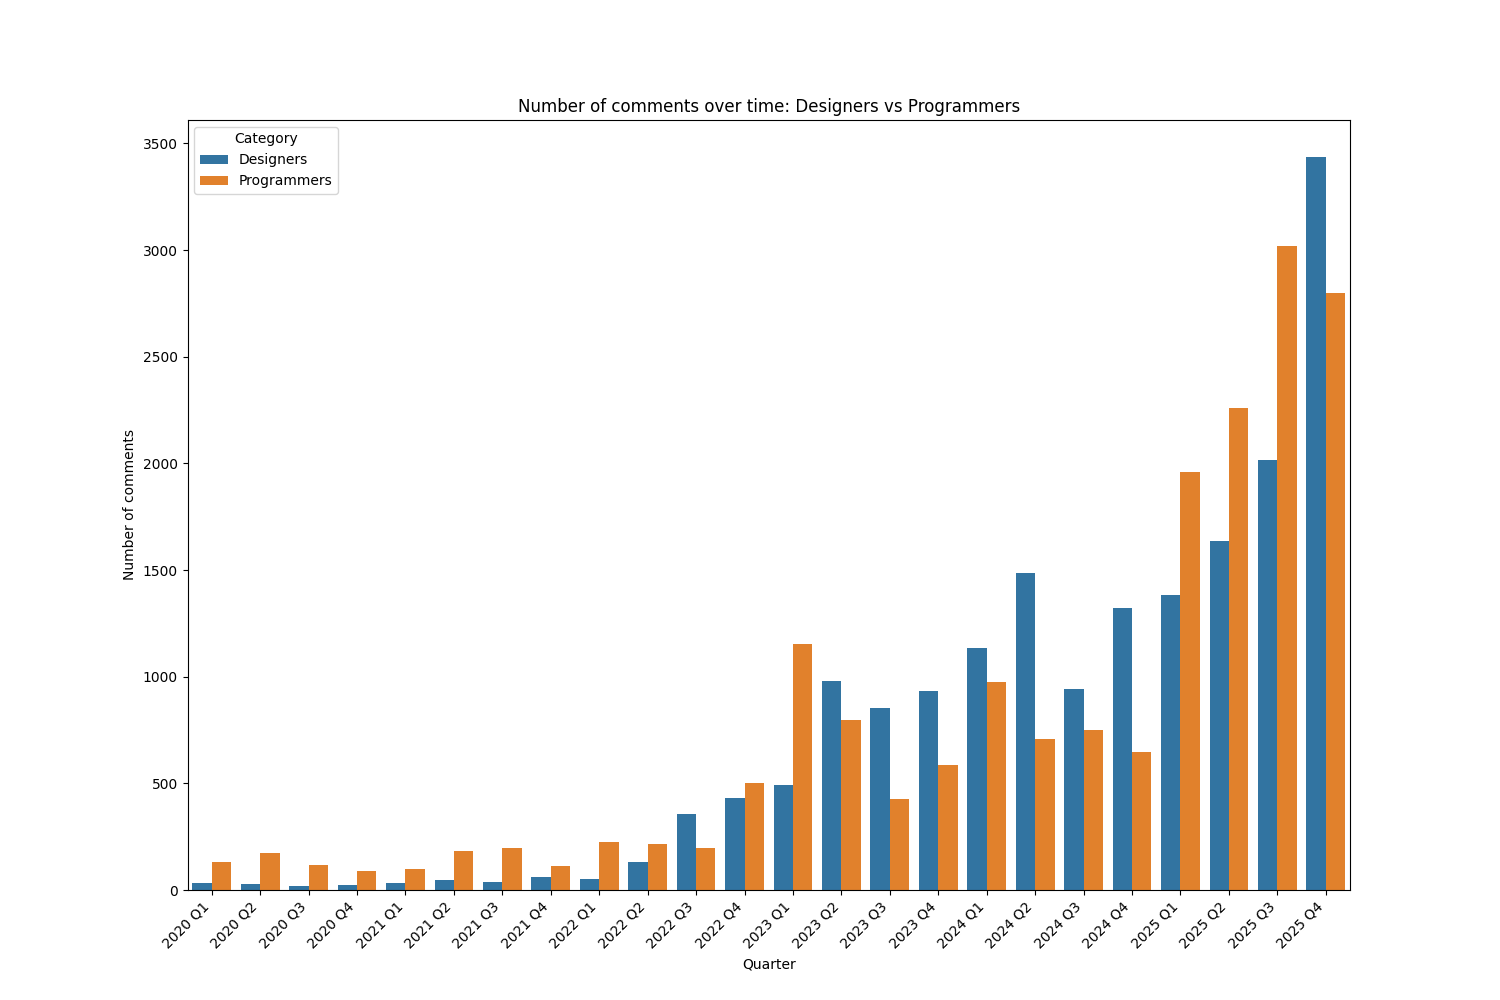
\includegraphics[width=0.95\linewidth]{Images/designers_vs_programmers_number_of_comments_over_time.png}
    \caption{Number of comments per quarter of each year examined.}
\label{fig:number_comments}
\end{figure}

\subsection{Cleaning and Preprocessing}
Before an in-depth analysis, a critical step in data collection is cleaning or data preprocessing. Essentially, it is a way of converting the raw, noisy, unstructured data into a more organized, clean format. Although this results in a reduction of the volume in the data, the idea is to maintain the most important parts of speech (PoS) that maintain the general idea. Proceeding with a good extraction and cleaning of data improves efficiency, model accuracy, and ensures consistency in the analysis of the gathered information.

The main parts of speech chosen to use include:
\begin{itemize}
    \item Nouns: which represent specific concepts in the communities, such as code, automation, efficiency on one side; or creativity, workflow, aesthetics on the other;
    \item Verbs: which represent a certain position and agency, including examples like assist, enhance, or threaten, and replace;
    \item Adjectives: which help represent a specific orientation; either positively powerful, efficient, or negatively dangerous, limiting.
\end{itemize}
The model used to complete this step is spaCy \cite{b15}. spaCy is a free open-source library for Natural Language Processing (NLP) on large volumes of text at high speeds. Sentences were converted into lemmas, and lemmas were then associated with a part of speech. Lemmatization is a technique in NLP that uses vocabulary morphological analysis to ensure a valid and meaningful result.

Although spaCy supports a wide range of PoS, it does not actively provide hashtags, mentions, links, but most importantly, emoticons or emojis. Emoticons are extremely important to know in this dataset, as these representational characters easily express emotions in an easier and more frequently used way. To check for these values, a conversion of emojis was done using Spacymoji, an extension of spaCy focused on converting emojis to their descriptions, in order for this to be processed correctly.

The PoS filtering is only applied to the semantic network, so as not to have too much clutter of words, while the sentiment is applied to the whole comment, where its context is important. The objective of the semantic network is to see the most important (frequency weighted with upvotes) words used inside the comments, while pairing words to each other (textual similarity, correlation, and co-occurrence). Reddit’s dataset does not contain explicit relational markers; therefore, finally, the networks constructed with the filtered and cleaned data rely primarily on these semantic relationships.

\subsection{Ethical considerations}
The data collection process closely followed Reddit’s terms of service and standard ethical guidelines. All gathered text was publicly available and accessible data from the Reddit platform. Usernames are identifiable only on the CSV file, but are not directly targeted or shared to protect the user’s privacy or personal information. The dataset and graphs are anonymized and generalized to prevent the identification of specific information. This did not affect or create any type of bias in the research. Particular care was taken to protect all rights and minimize harm from the interpretation of the findings.

\section{Language Processing (Alessandra)}
The numerous comments identified in the collected datasets are processed through language processing techniques. This approach makes it possible to overcome the qualitative and fragmentary nature of individual posts, in order to obtain a scientific measurement of social perception. The data processing follows this logic and is articulated in a detailed analysis, which is carried out through the investigation of topic analysis, emotion analysis and sentiment analysis. Finally, the analysis is widened by creating and investigating the semantic networks for the two communities.

\subsection{Topic Analysis}
Models and algorithms were employed in order to transform the raw data into thematic groups. In particular, BERTopic and Louvain were used.

BERTopic is a model based on the semantic content of documents; by using vector representations of text, it groups documents into coherent topics, based on semantic similarities and, therefore, their meaning.

By contrast, Louvain is an algorithm based on modularity, a metric connected to the network structure on which the clustering is based: it identifies what nodes are strongly connected to one another, in order to form groups.

This type of topic analysis makes it possible to understand what is being talked about in each community, with greater precision than the initial broad topic, which concerned the integration of AI into one’s work. It also allows for the identification of the topics that are of greatest interest and generate the most debate within each of the two communities considered.

\subsection{Emotion Analysis}
Emotion analysis is used to investigate the specific emotions of users, going beyond simple opinions and capturing their psychological reactions.\\
The emotions taken into consideration were chosen by selecting three that are more relevant to skepticism and three that are more consistent with enthusiasm. Instead, emotions that might be ambiguous have been avoided, in order to obtain clearer and more meaningful results.\\
For the first category (skepticism) the emotions taken into account are:
\begin{itemize}
    \item Anger: irritation and hostile reaction toward AI;
    \item Fear: anxiety related to the unpredictable consequences of AI and possible human replacement;
    \item Pessimism: negative expectations about the future effects of AI.
\end{itemize}
For the second category (enthusiasm) the emotions considered are:
\begin{itemize}
    \item Joy: enthusiasm about the benefits offered by AI;
    \item Trust: positive level of confidence in AI’s accuracy or fairness;
    \item Optimism: positive expectations about the future effects of AI.
\end{itemize}

\subsection{Sentiment Analysis}
The usefulness of sentiment analysis is to investigate the evolution of sentiment over time within the two communities. This has been done both on a quarterly and yearly basis. The examination of sentiment is structured in three complementary phases:
\begin{enumerate}
    \item Unweighted sentiment analysis: in this first phase, each comment is assigned the same weight in the analysis; therefore, the number of upvotes is disregarded. The objective is to observe the overall trend of sentiment within the two communities;
    \item Weighted sentiment analysis: in this second phase, each comment is assigned a weight consistent with the number of upvotes it has received; consequently, comments with a higher number of upvotes become more influential. The objective is to understand which sentiment is promoted by the most important comments and whether this is consistent with the general sentiment analyzed in the initial phase;
    \item Yearly sentiment analysis: in this third phase, the results are examined on a yearly basis. The objective is to observe the evolution of sentiment in the long term.
\end{enumerate}
Together, these approaches make it possible to understand the sentiment evolution on a deeper level, highlighting fluctuations but, more importantly, long-term trends.

\subsection{Semantic Networks}
Semantic networks make it possible to map precisely what words are used within each community and understand the relationship between concepts. In order to make the complex graphs clearer and legible, overcoming the noise of Reddit’s data, the nodes have been filtered using their degree, allowing for the isolation of the most significant lexicon. The PageRank algorithm has also been applied to define the importance of each individual node and their hierarchy: this allows them to identify the most relevant concepts. Through these operations, it is possible to obtain semantic networks that organise the discourse into thematic clusters that can be visually observed and then interpreted.

\section{Network Characteristics (Giacomo)}

Before any kind of further analysis, we need to define the networks that will be used, both for the programmers' subreddit and for the designers' subreddit. For each of them, we create a probability matrix $P_{w|d}$ linking documents ($d$) to words ($w$) using the following steps:
\begin{enumerate}
    \item calculate the frequency matrix $f$ of each word inside each of the documents defining rows and columns, respectively;
    \item calculate the probability that each word is obtained when picking a word randomly inside of a document, defining the probability matrix $P$, with each element $P_{ij}$ being defined as the number of frequencies for the specific word with index $i$ divided by the total frequency of words $n$ inside the document with index $j$;
    \begin{align*}
        P_{ij} = \frac{f_{ij}}{\sum_{k=1}^n f_{kj}}
    \end{align*}
    \item apply a weight $w_j$ to each document $d_j$ based on the upvotes $u(d_j)$ associated with it. This is done to allow incorporation of upvotes inside the probability matrix, so that more important documents, defined as having more upvotes, have a higher probability; 
    \begin{align}
        w_j = \log_{10}(1 + \vert u(d_j) \vert)
        \label{eq:documentWeight}
    \end{align}
    \item apply the obtained weights to the probability matrix $P$ and normalize them with respect to the sum of the weights, so that each element of it has value $0 \le P_{w \vert d, ij} \le 1$, finally defining $P_{w \vert d}$;
    \begin{align*}
        P_{w \vert d, ij} = \frac{w_j}{\sum_{j=1}^m w_j}P_{ij}
    \end{align*}
\end{enumerate}

From this matrix $P_{w|d}$, we need the projection of documents on the matrix, which links documents to documents, allowing for an analysis on the relationships between documents; this matrix will define the documents' networks.
\begin{align*}
    P_{dd} = P_{w \vert d}^\text{T} \cdot \text{diag}(p_{w\vert d} \cdot \mathbf{1}) \cdot P_{w \vert d}
\end{align*}

We can also define the projection of words on the matrix, which links words to words, allowing for an analysis on the relationships between words across the whole batch of documents; this matrix will define the words' network.
\begin{align*}
    P_{ww} = P_{w \vert d} \cdot \text{diag}(p_{w\vert d}^\text{T} \cdot \mathbf{1}) \cdot P_{w \vert d}^\text{T}
\end{align*}

These networks are all undirected and unsigned. For parts of the analysis, such as degree centrality and semantic networks, we will use Gephi \cite{b16}, which is an open-source software for exploring and manipulating networks, that also allows us to calculate statistics and define a layout for information display. 

\subsection{Degree Centrality}

For the programmers' network, the average degree is $\langle k \rangle_p = 1054.02$, while for the designers' network $\langle k \rangle_d = 1043.08$, calculated through the "average degree" Gephi function.

Since it also calculates the degree of each node, we can use them to find out if networks show a particular behavior, such as following the power-law. We can define the power-law as:
\begin{align*}
    p(k) = C \cdot k^{-\gamma}
\end{align*}
where $C$ is a constant and $\gamma$ defines the slope.

We obtained $\gamma$ using the powerlaw module in Python \cite{b17}, which uses a Machine Learning approach to maximize the likelihood of each possible value with the available degrees in the nodes.\\
Then, we can determine $C$ through the approximated normalization condition: 
\begin{align*}
    \int_{k_{\min}}^\infty p_k dk = C \cdot \frac{k_{\min}^{-(\gamma - 1)}}{\gamma - 1} = 1
\end{align*}
which results in:
\begin{align*}
    C = \frac{\gamma - 1}{k_{\min}^{-(\gamma - 1)}}
\end{align*}
with $k_{\min}$ being the minimum degree inside the network. 

Knowing this, we can show the degree distributions for each of the documents' networks.

% Image designers power-law
\begin{figure}[H]
    \centering
    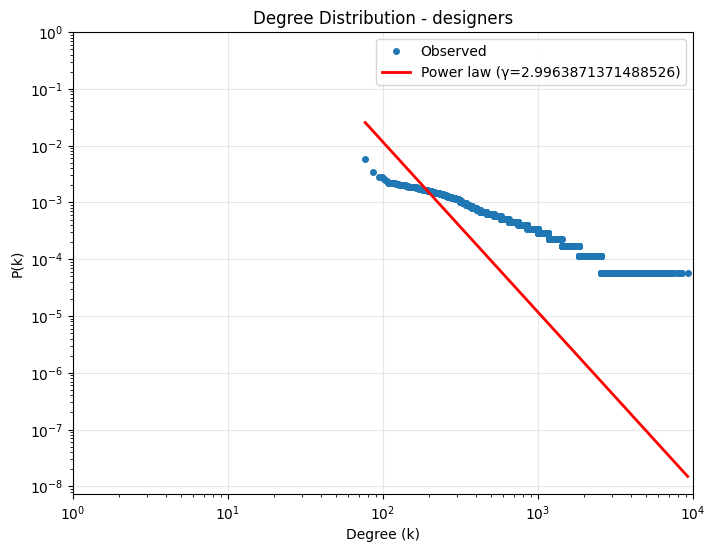
\includegraphics[width=0.95\linewidth]{Images/designers_powerlaw.png}
    \caption{Degree distribution of the designers' network with powerlaw.}
    \label{fig:des_powerlaw}
\end{figure}

% Image programmers power-law
\begin{figure}[H]
    \centering
    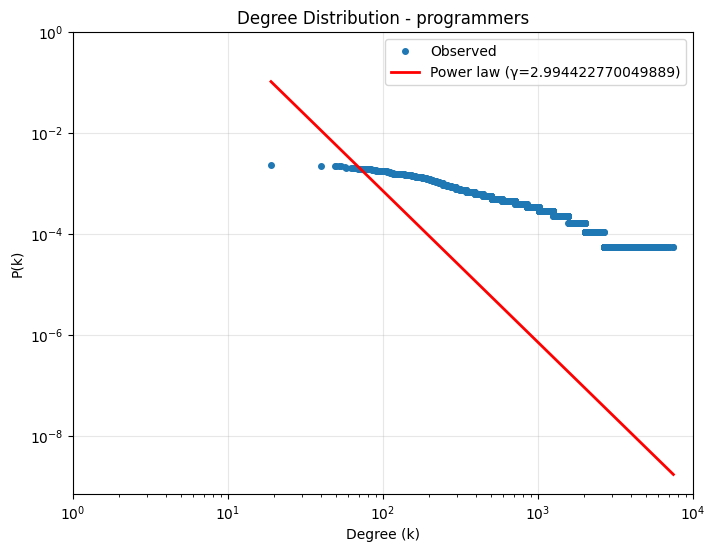
\includegraphics[width=0.95\linewidth]{Images/programmers_powerlaw.png}
    \caption{Degree distribution of the programmers' network with powerlaw.}
    \label{fig:prog_powerlaw}
\end{figure}

We can see that, for both networks, the power-laws show they are at the limits of a scale-free regime, with $\gamma \approx 2.997$ for the designers and $\gamma \approx 2.994$, and therefore we can regard them as being in a scale-free regime. This means that both networks are close to being indistinguishable from a random network, but they still define an ultra-small world. Therefore, the mean distance between nodes in the network is definable as:

\begin{align*}
    \langle d \rangle \sim \ln\ln N
\end{align*}

where $N$ defines the number of nodes inside the network.

For the programmers' network, this mean distance between two nodes is approximately $\langle d\rangle_p \approx 2.283$, while for the designers' network, this value is approximately $\langle d\rangle_d \approx 2.281$.

\subsection{Homophily}
Homophily is a phenomenon where similar users tend to connect with each other. To measure homophily inside a network, we can define the assortativity coefficient through the relative method inside the NetworkX library in Python \cite{b18}. For the documents' network, the assortativity coefficients are, then, $\mu_d = -0.1045$ and $\mu_p = -0.1267$, showing a slight dis-assortivity for both networks, which means that the effect is opposite with respect to homophily: higher degree nodes tend to interact with lower degree nodes.

% Image designers correlation regression
\begin{figure}[H]
    \centering
    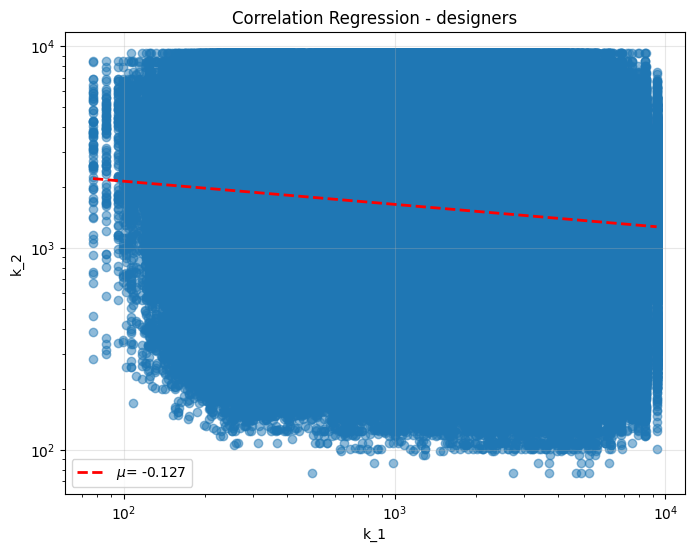
\includegraphics[width=0.95\linewidth]{Images/designers_correlation_regression.png}
    \caption{Degree correlation of the designers' network with regression, quantifying assortativity.}
    \label{fig:des_assortativity}
\end{figure}

% Image programmers correlation regression
\begin{figure}[H]
    \centering
    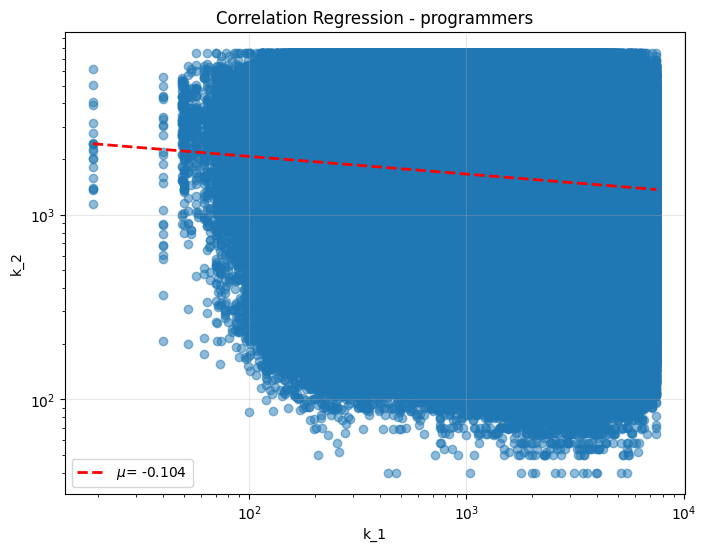
\includegraphics[width=0.95\linewidth]{Images/programmers_correlation_regression.png}
    \caption{Degree correlation of the programmers' network with regression, quantifying assortativity.}
    \label{fig:prog_assortativity}
\end{figure}

\section{Topic Analysis (Tommaso \& Charlie)}
To investigate how enthusiasm and skepticism toward AI are articulated within professional discourse, we performed topic analysis on the document networks of programmers and designers. Topic identification was conducted using two complementary approaches: Louvain community detection on the document to document projection network and BERTopic on semantic embeddings of the documents. While the two methods rely on different principles, structural connectivity and semantic similarity, they converge on a coherent set of dominant discursive clusters.

\subsection{Algorithms}
Since our projection network on documents is undirected, the first approach we implement to obtain a community clustering is the Louvain algorithm  (Blondel, Guillaume, Lambiotte, \& Lefebvre, 2008 \cite{b19}). It is based on the modularity metric, which measures the density of links inside communities compared to the links between communities. Modularity in undirected networks is defined as:

\begin{align}
    Q = \text{trace}(\mathbf{C} (\mathbf{A} - \mathbf{d} \: \mathbf{d}^T) \mathbf{C}^T) \label{eq:modularity}
\end{align}

where $\mathbf{C}$ is the community assignment matrix and $\mathbf{A}$ is:
\begin{align*}
    \mathbf{A} = \frac{\mathbf{A}_0}{D_0} \quad \text{with} \quad D_0 = \mathbf{1}^T \: \mathbf{A}_0 \: \mathbf{1}
\end{align*}
where $\mathbf{A}_0$ is the original adjacency matrix of the network.\\
The Louvain algorithm proceeds in two main phases:
\begin{enumerate}
    \item Local optimization: the modularity $\mathbf{Q}$ is increased using local changes of community assignment. Specifically, a node $i$ is moved from its current community to one of the communities of its neighbors. After the move, the change in modularity is computed as:
    \begin{align*}
        \Delta \mathbf{Q} = 2 \mathbf{c}^T (\mathbf{a}_i - \mathbf{d}_i \mathbf{d})
    \end{align*}
    Only the moves that maximize $\Delta \mathbf{Q}$ are accepted.
    \item Community aggregation: once local optimization converges, the communities found in the previous step are used to build a new network of communities with a normalized adjacency matrix $\mathbf{P}_{CC}$:
    \begin{align*}
        \mathbf{P}_{CC} = \mathbf{C} \: \mathbf{A} \: \mathbf{C}^T
    \end{align*}
    The two phases are then repeated iteratively until the modularity $\mathbf{Q}$ reaches a maximum and the community structure stabilizes.
\end{enumerate}
These communities are interpreted as topics.

To have a more semantically meaningful perspective we use the BERTopic model \cite{b20}, which converts the input documents $d_i$ to embeddings $\mathbf{x}_i \in \mathbb{R}^n$ that capture their semantic content.

The embeddings are then projected into a lower-dimensional space using UMAP (Uniform Manifold Approximation and Projection) \cite{b21} where clusters of semantically similar documents can be computed. The clustering is performed with HDBSCAN \cite{b22} and each cluster corresponds to a potential topic. To interpret these clusters, BERTopic computes a class based (c-TF-IDF) for each topic.\\
From each of the two methods we obtain:
\begin{itemize}
    \item the word-topic distribution matrix $\mathbf{P}_{w,c} \in \mathbb{R}^{|W|\times|C|}$, where $|W|$ is the vocabulary size and $|C|$ is the number of topics;
    \item the topic adjacency matrix $\mathbf{P}_{CC} \in \mathbb{R}^{|C|\times|C|}$;
    \item the vector assigning each document to a topic $\mathbf{C} \in \{1,\dots,|C|\}^N$, where $N$ is the number of documents;
    \item the vector representing the fraction of documents assigned to each topic $\mathbf{p}_c \in \mathbb{R}^{|C|}$ with $\sum_c p_c(c)=1$
\end{itemize}

\subsection{Evaluation metrics}

In order to obtain a measure of the quality of the topic recognition we compute, for each topic assignment, the following metrics:

\begin{itemize}
    \item Normalized Mutual Information (NMI): evaluates how much the word distribution is informative w.r.t. the topic assignment. We compute it as:
    \begin{align*}
        \text{NMI} = \frac{1}{H(\mathbf{C})} \sum_{w, c} \mathbf{P}_{WC}(w,c) \log\frac{\mathbf{P}_{WC}(w,c)}{P_w \: P_c}
    \end{align*}
    \item Normalized cut (Ncut): measures how well separated the topics are given the document network structure. We compute it as:
    \begin{align*}
        \text{Ncut}(\mathbf{C}) = \sum_{k=1}^{K} \frac{\text{cut}(C_k, \overline{C}_k)}{\text{vol}(C_k)}, \quad 
        \text{vol}(C_k) = \sum_{i \in C_k} k_i
    \end{align*}
    where $\overline{C}_k$ is the set of nodes not in $C_k$.
    \item Modularity (Q): is the number of edges falling within communities minus the expected number in an equivalent network with edges placed at random. We compute it as seen in eq.\eqref{eq:modularity}.
    \item Infomap: is an information-theory metric that evaluates how much the topic assignment compresses the information flow. We compute it as:
    \begin{align*}
        L \gtrsim H(\mathbf{C}) = \sum_i p_i \log_2 \frac{1}{p_i}
    \end{align*}
    \item Community balance (com): measures how evenly the documents are split across different topics. We compute it as:
    \begin{align*}
        \text{com} = \frac{- \sum_{c=1}^{K} \mathbf{p}_c(c) \log \mathbf{p}_c(c)}{\log K}
    \end{align*}
\end{itemize}
These metrics were combined into a score, computed as:
\begin{align*}
    S = \text{NMI} + \text{Q} + \text{Infomap} + \text{com} - \text{Ncut}
\end{align*}

\subsection{Practical approach}
The Louvain and BERTopic algorithms were applied iteratively on the document network obtained from the designers and the programmers network, with the following stopping criteria:
\begin{itemize}
    \item The algorithms stop if a topic assignment satisfies all of the following conditions:
    \begin{align*}
        &\text{NMI} > 0.15 \\
        &\text{Q} > 0.4 \\
        &\text{Ncut} < 0.2 \\
        &\text{Infomap} > 0.5 \\
        &\text{com} > 0.5
    \end{align*}
    \item the maximum number of iterations (set to 10) is reached.
\end{itemize}
In both cases the best run for each algorithm, determined according to the overall score $S$, was retained. The results are shown in Tables \ref{tab:des_topic_metrics} and \ref{tab:prog_topic_metrics}.
\begin{table}[htbp]
\centering
\caption{Designers network results}
\label{tab:des_topic_metrics}
\begin{tabular}{l c c c c c c}
\hline
Method & NMI & Q & Ncut & Infomap & com \\
\hline
BERTopic & 0.293 & 0.003 & 0.810 & 0.011 & 0.053 \\
Louvain & 0.123 & 0.081 & 0.785 & 0.081 & 0.846 \\
\hline
\end{tabular}
\end{table}

\begin{table}[htbp]
\centering
\caption{Programmers network results}
\label{tab:prog_topic_metrics}
\begin{tabular}{l c c c c c c}
\hline
Method & NMI & Q & Ncut & Infomap & com \\
\hline
BERTopic & 0.170 & 0.040 & 0.931 & 0.081 & 0.553 \\
Louvain & 0.124 & 0.090 & 0.710 & 0.737 & 0.959 \\
\hline
\end{tabular}
\end{table}
For the best topic assignments, we computed for each topic $c$:
\begin{itemize}
    \item The top 100 words with non-zero conditional probability $P_{w|c}$ of belonging to $c$ ordered using the PageRank $PR(w)$ computed in the word network
    \item A wordcloud representing the words of each of the topic with a size proportional to the combined relevance $v$ computed as:
    \begin{align*}
        v = P_{w|c} \cdot PR(w)
    \end{align*}
    This score balances cluster-specific importance ($P_{w|c}$) and global structural centrality ($PR(w)$)
\end{itemize}

\subsection{Programmers}
In the programmers’ community, the identified topics are strongly centered on instrumental and task-oriented dimensions of AI usage. The largest clusters focus on code generation, debugging, problem solving, learning support, and system efficiency. AI is primarily framed as a functional tool that augments existing technical skills, enabling faster development cycles and improved productivity. Within these topics, enthusiasm is expressed through narratives of optimization and assistance, where AI is portrayed as a collaborator that reduces repetitive labor and accelerates learning. Skepticism, when present, is largely conditional rather than oppositional. It emerges in discussions concerning the reliability of AI-generated code, the transparency of training data, and legal or ethical issues such as copyright and data ownership. Importantly, these skeptical elements do not challenge the legitimacy of AI as a tool, but instead delimit its acceptable scope of use.

Overall, programmers' topic structure suggests a pragmatic form of polarization: enthusiasm dominates the discourse, while skepticism functions as a moderating force aimed at preserving technical control and professional standards.
\begin{figure}[H]
    \centering
    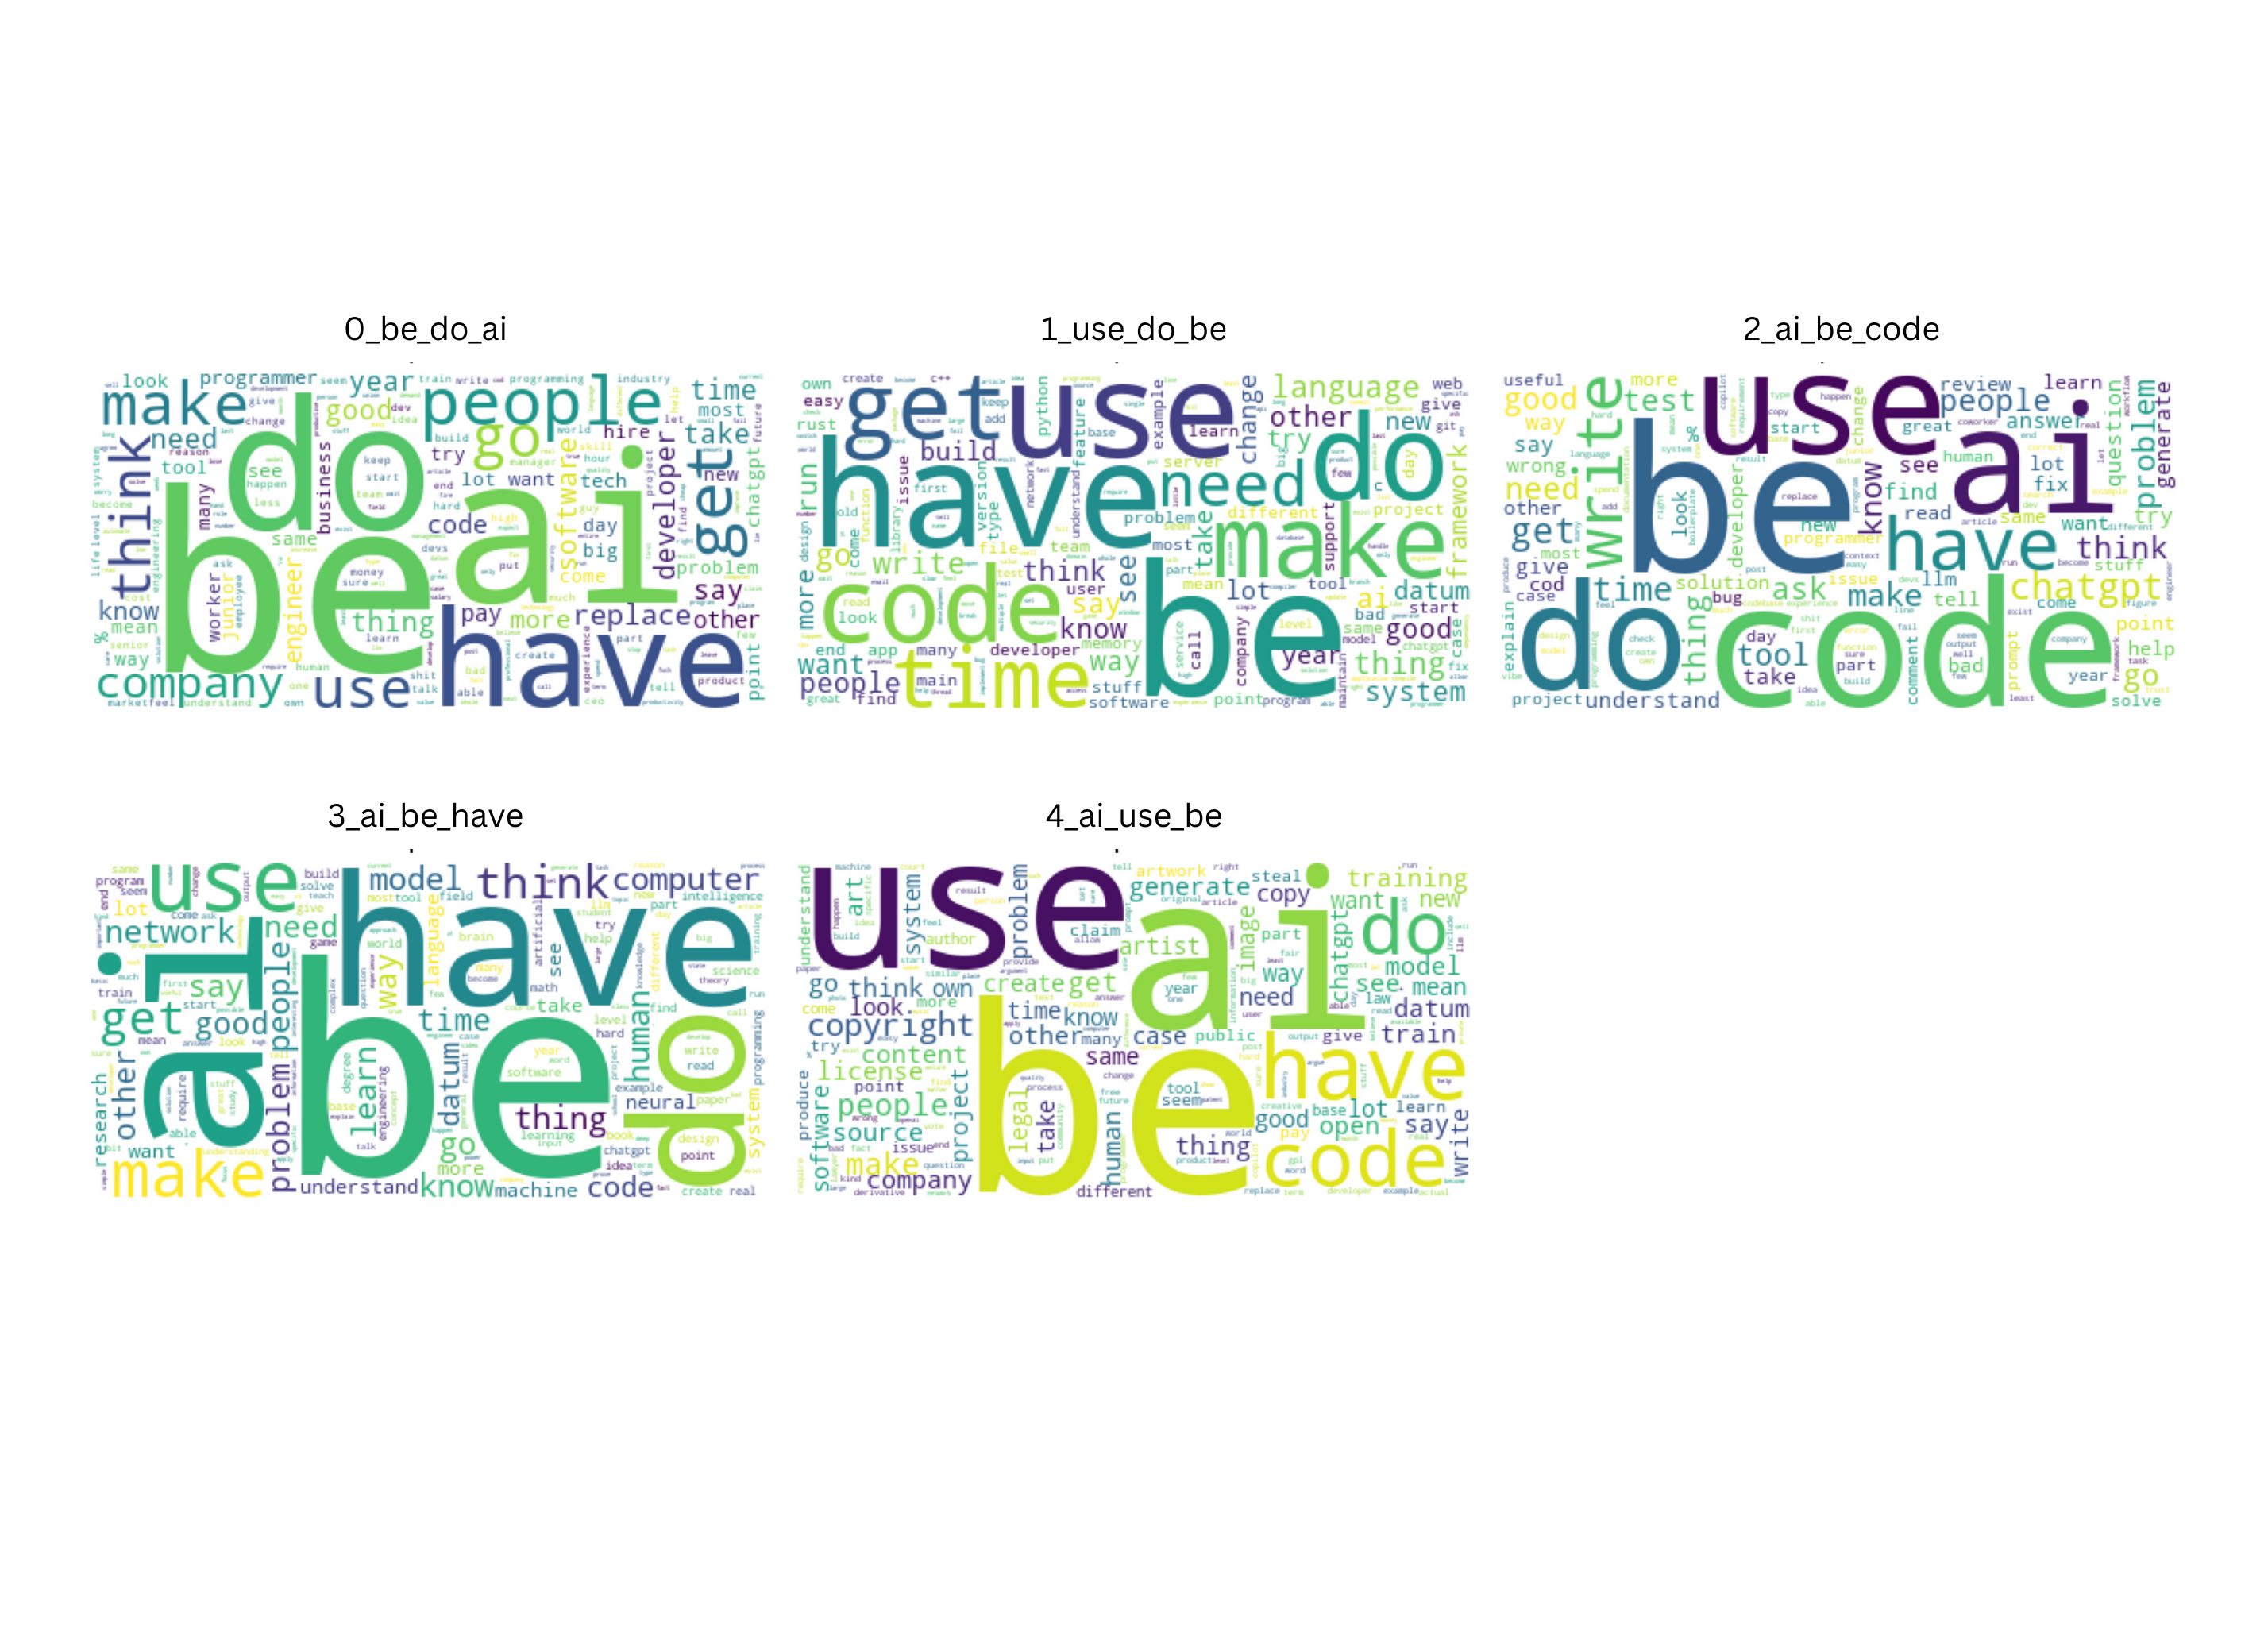
\includegraphics[width=0.95\linewidth]{Images/programmers_louvain_wordcloud_rename.png}
    \caption{Louvain wordclouds for programmers.}
    \label{tab:prog_louvain}
\end{figure}
\begin{figure}[H]
    \centering
    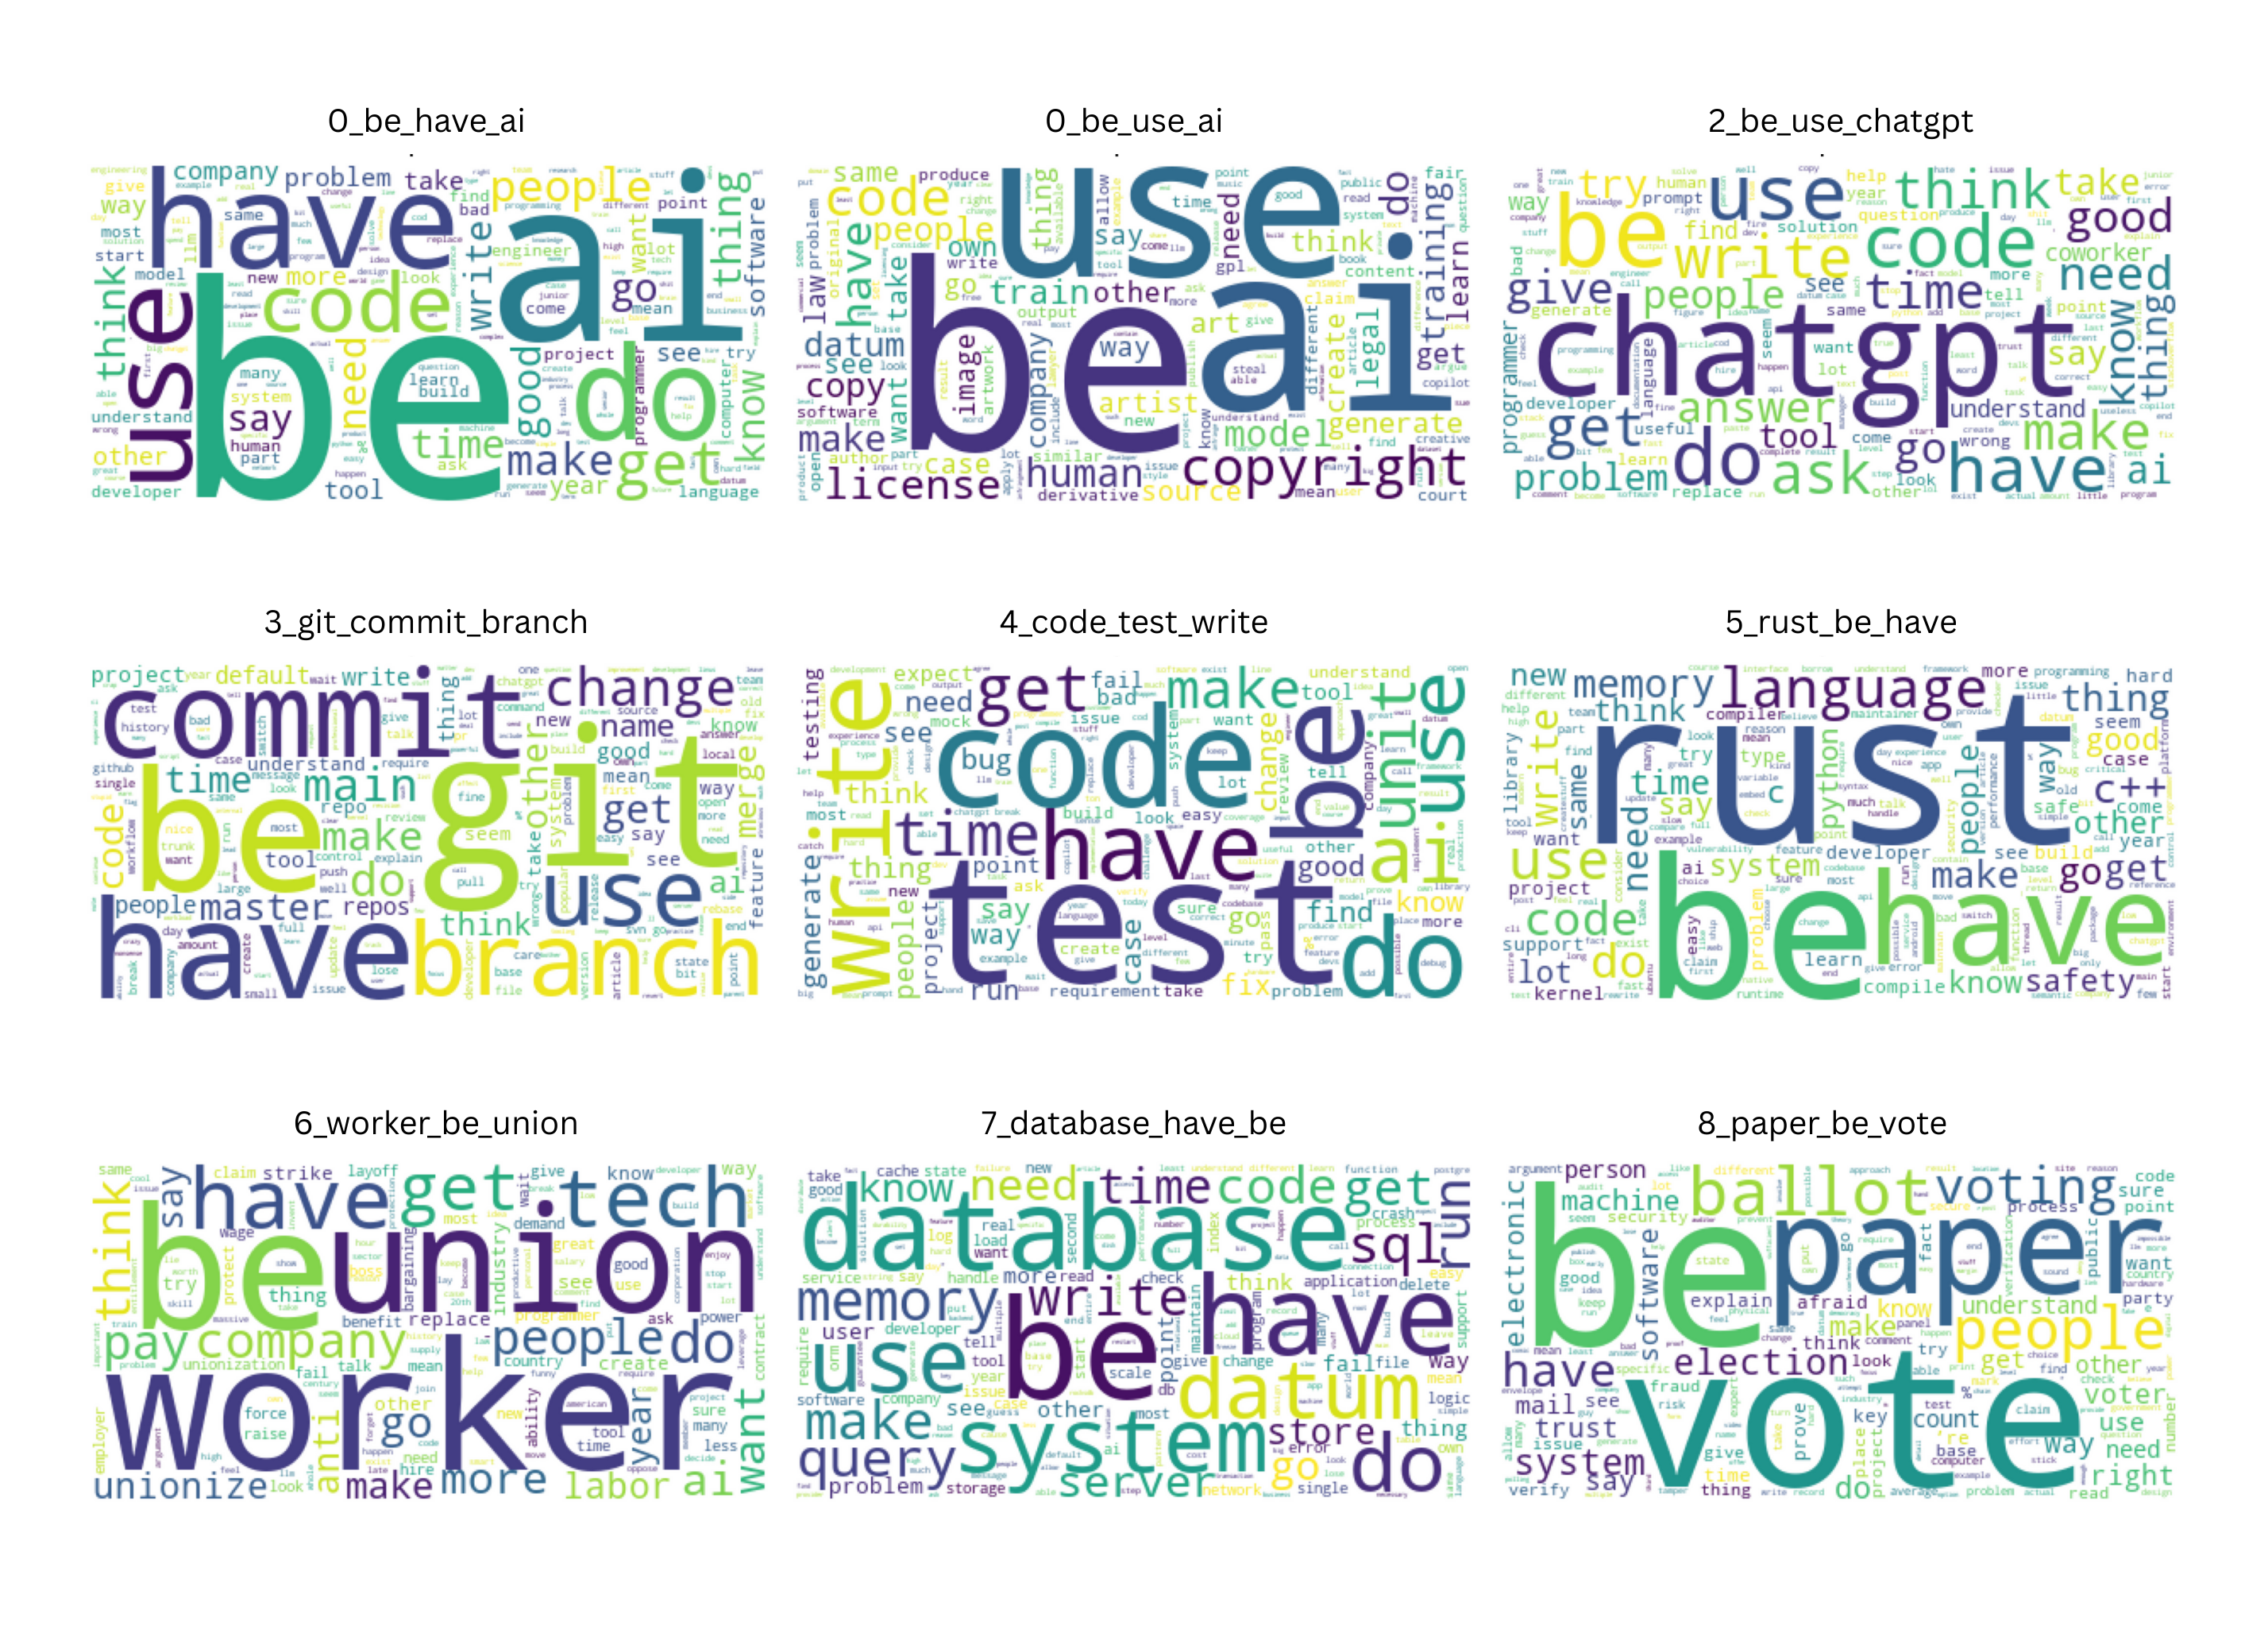
\includegraphics[width=0.95\linewidth]{Images/programmers_BERTopic_wordcloud_rename.png}
    \caption{BERTopic wordclouds for programmers.}
    \label{tab:prog_bertopic}
\end{figure}

\subsection{Designers}
In contrast, the designers community exhibits a topic structure that is more strongly oriented toward evaluation, interpretation, and professional identity. Dominant clusters revolve around feedback, portfolios, originality, context, and credibility. AI is not discussed merely as a productivity-enhancing tool, but as an actor that intervenes in processes traditionally grounded in human judgment and aesthetic sensibility. Enthusiastic discourse among designers tends to emphasize experimentation and inspiration, particularly in early-stage ideation. However, skepticism is more salient and deeply embedded within the topics themselves. Concerns about authorship, creative ownership, and the dilution of professional expertise recur across multiple clusters, indicating a structural tension between AI assistance and the symbolic value of human creativity.

Unlike programmers, designers do not simply question the performance or reliability of AI systems, rather, they question their legitimacy within creative practice. This produces a more cautious and reflexive form of engagement, where acceptance is negotiated rather than assumed.
\begin{figure}[H]
    \centering
    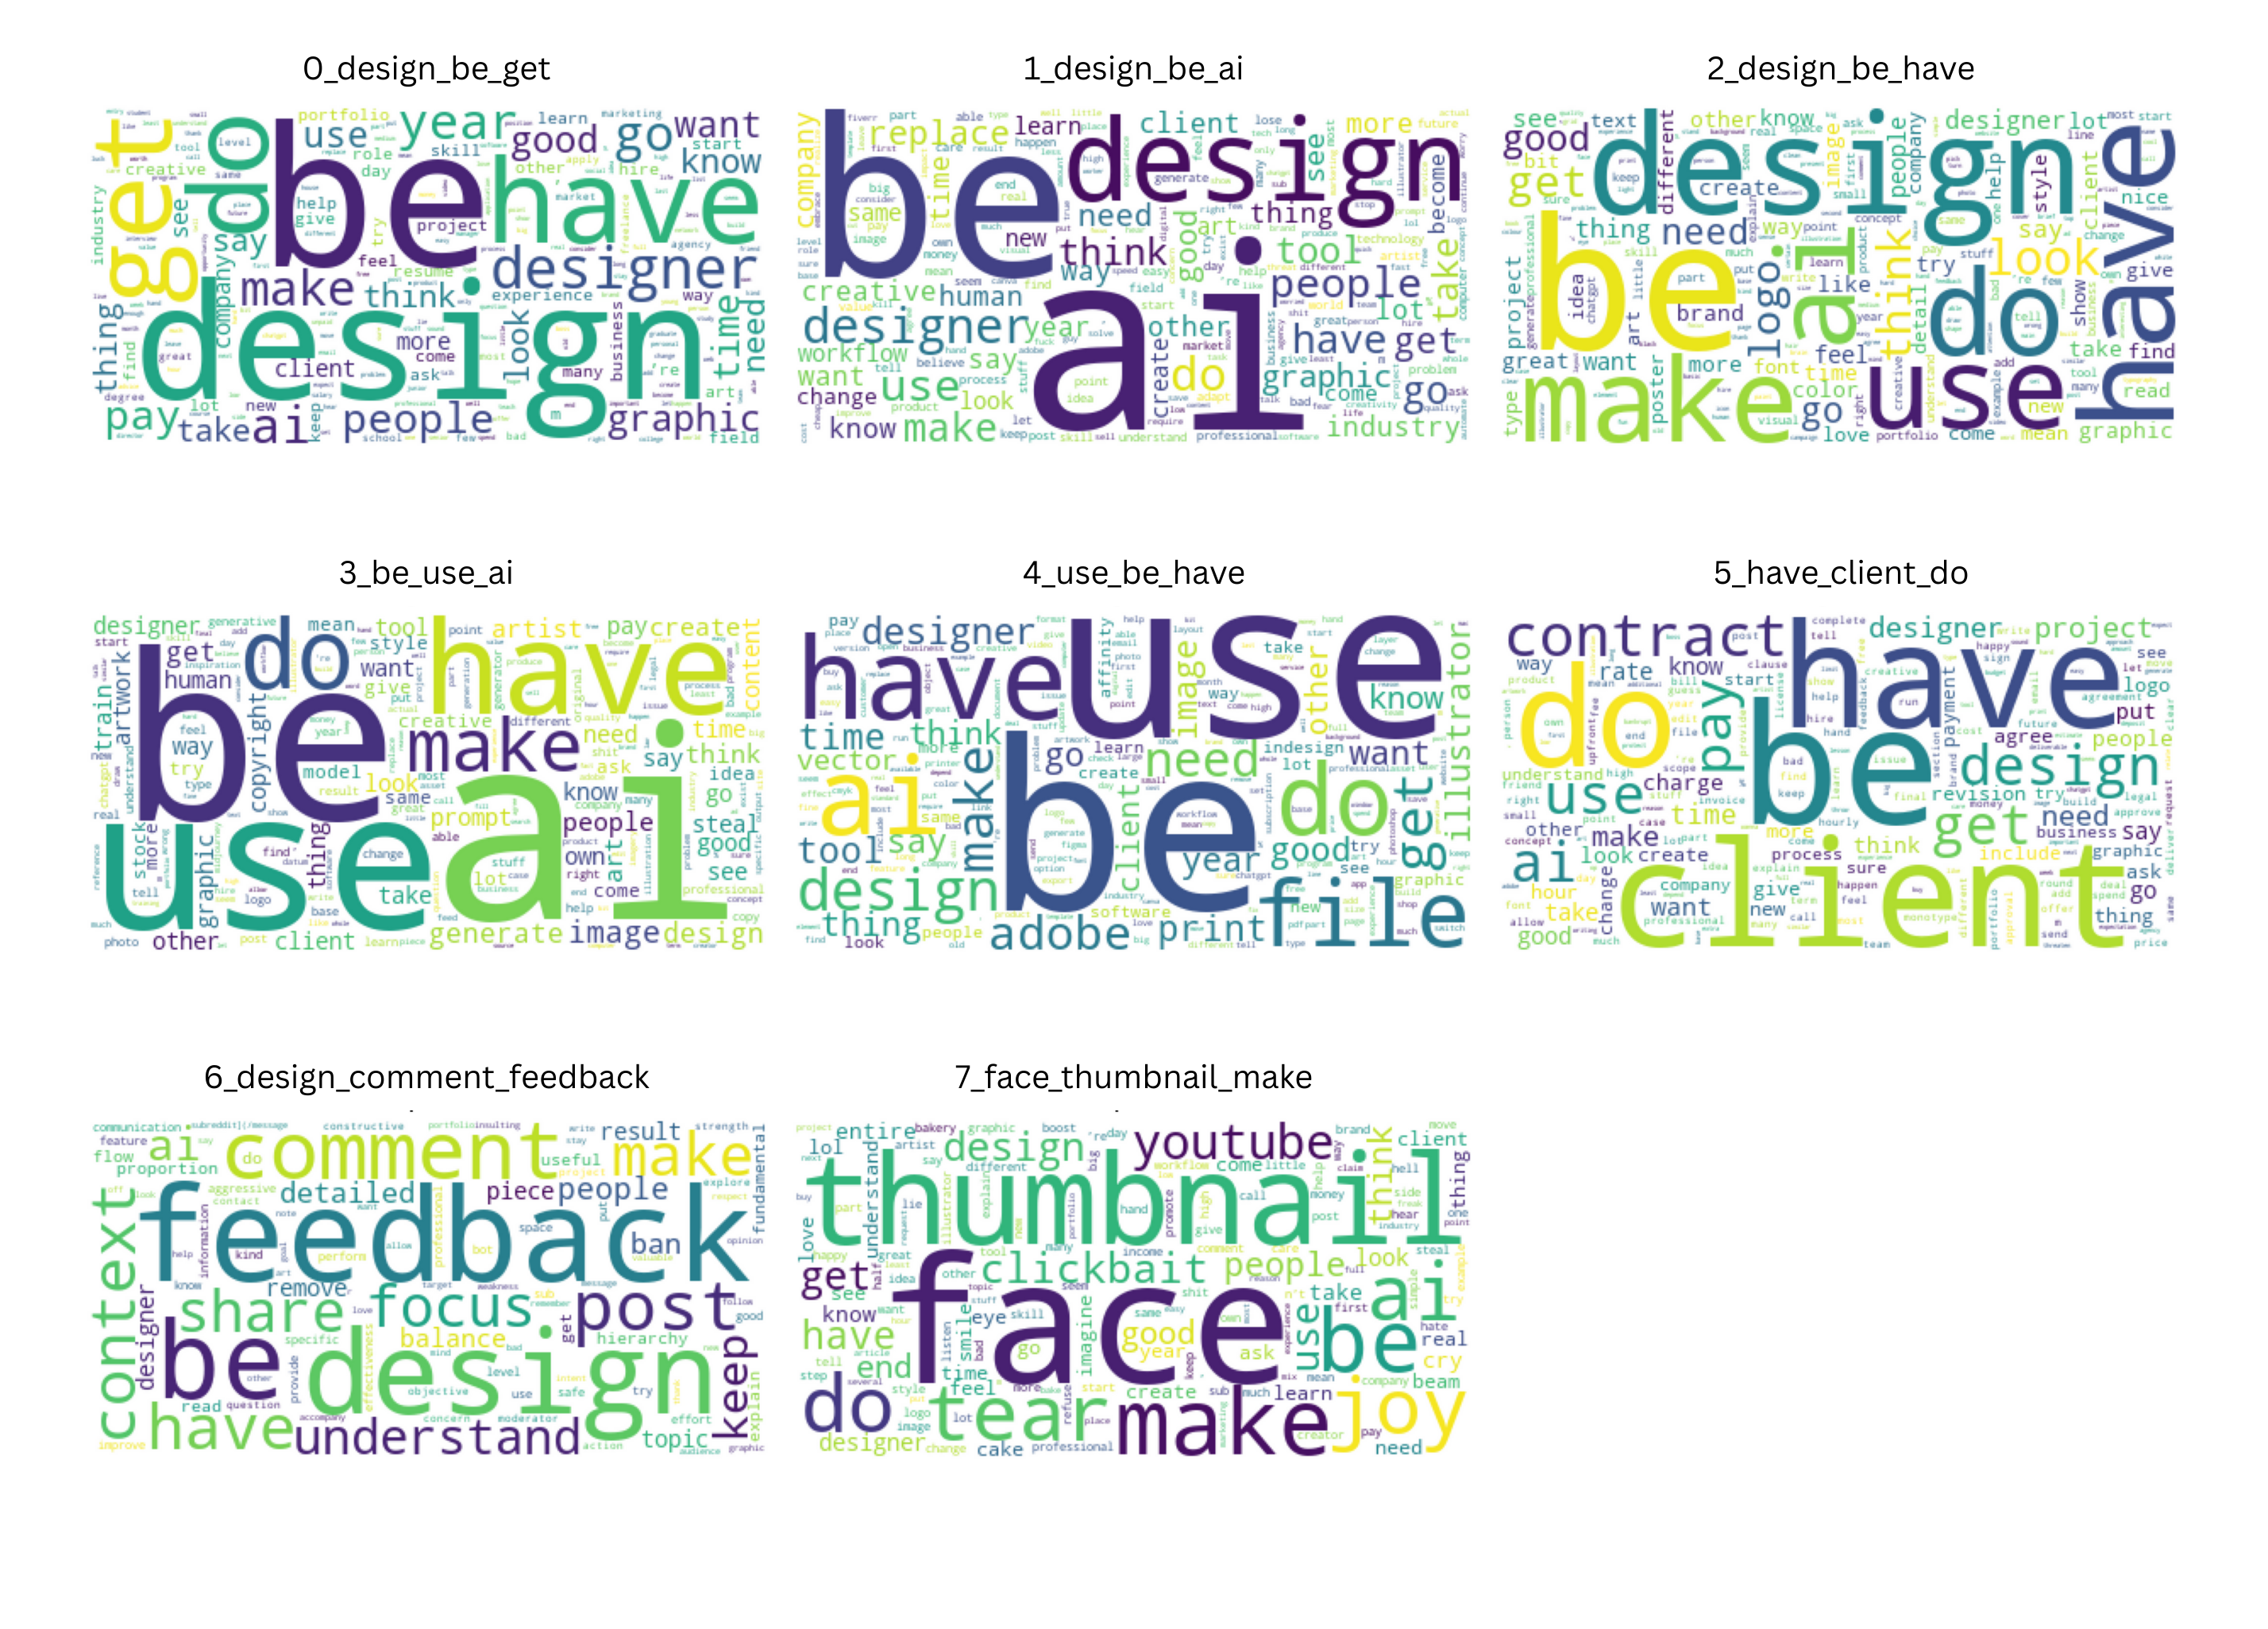
\includegraphics[width=0.95\linewidth]{Images/designers_louvain_wordcloud_renamed.png}
    \caption{Louvain wordclouds for designers.}
    \label{tab:des_louvain}
\end{figure}
\begin{figure}[H]
    \centering
    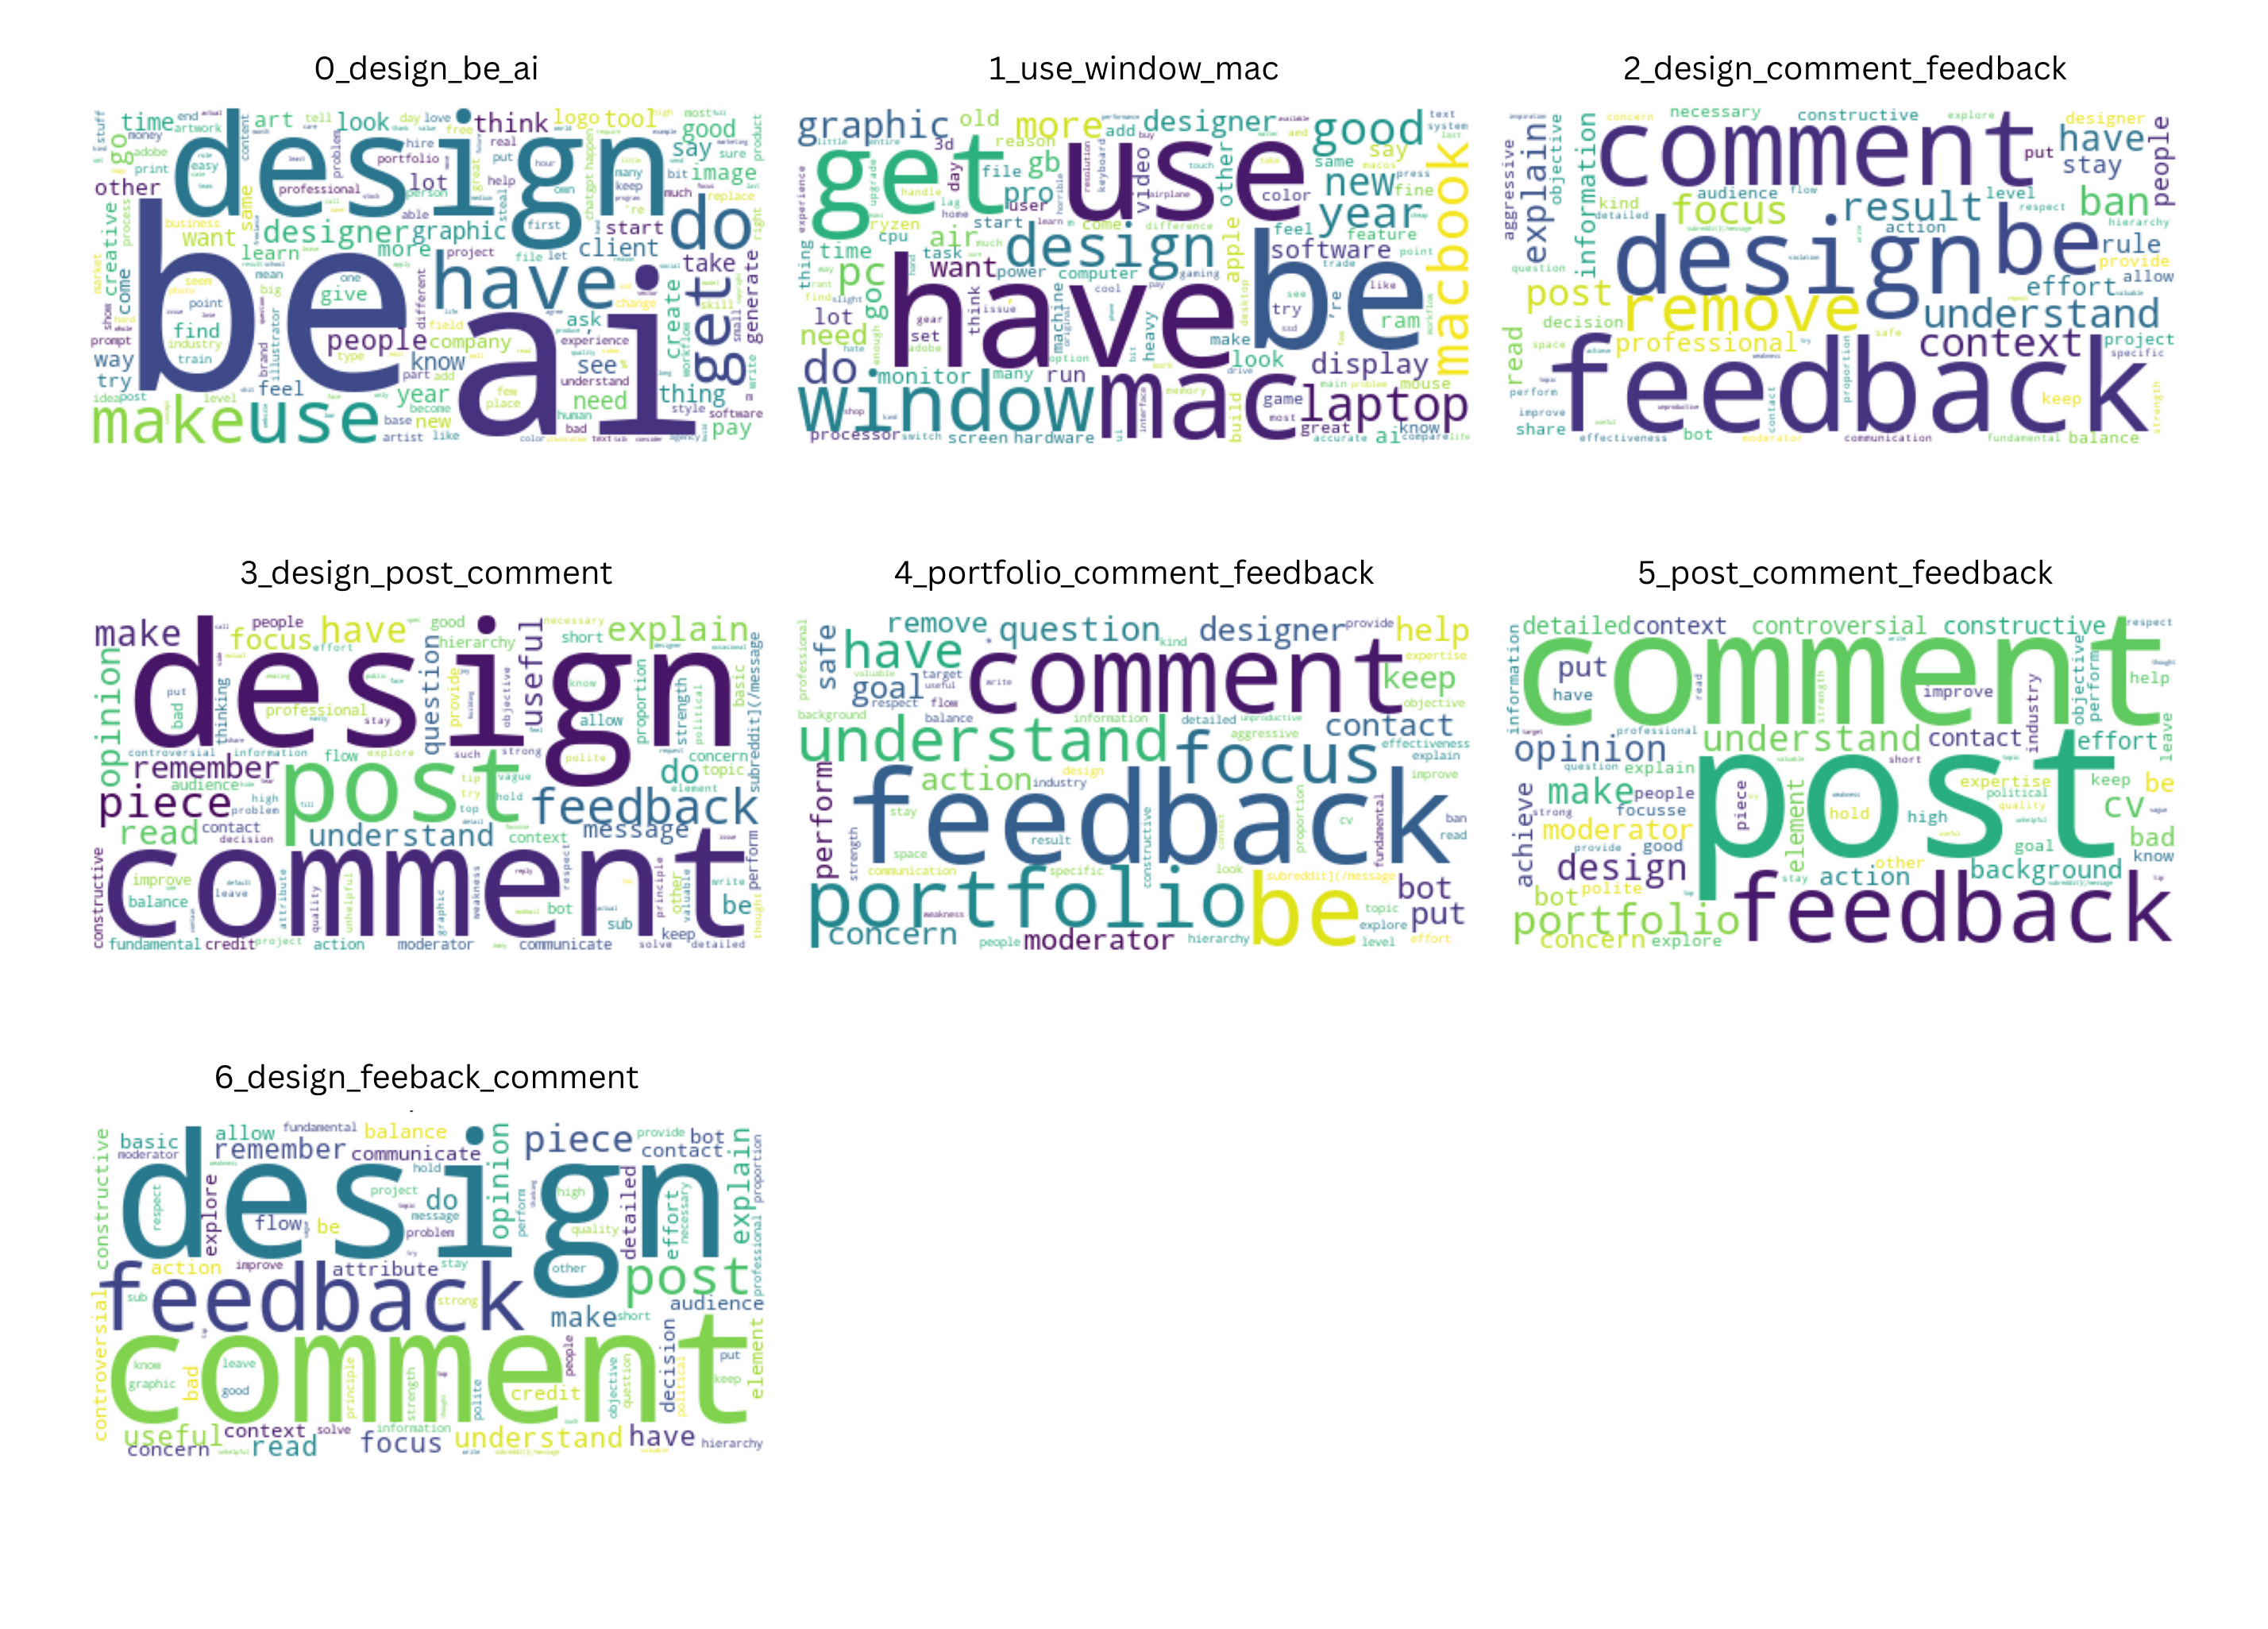
\includegraphics[width=0.95\linewidth]{Images/designers_BERTopic_wordcloud_renamed.png}
    \caption{BERTopic wordclouds for designers.}
    \label{tab:des_bertopic}
\end{figure}

\subsection{Differences}
Comparing the two communities, topic analysis reveals that polarization toward AI is shaped by distinct occupational logics. Programmers’ topics are organized around problem-solving efficiency and technical control, leading to a discourse where enthusiasm is structurally dominant and skepticism remains secondary. Designers’ topics, by contrast, are organized around evaluation and identity, producing a discourse in which skepticism is more pervasive and intertwined with professional self-definition. 

These differences suggest that polarization does not arise solely from attitudes toward AI as a technology, but from how AI intersects with the core values and evaluative criteria of each profession. Topic analysis thus provides evidence that enthusiasm and skepticism are not randomly distributed opinions, but are embedded in the semantic and social organization of professional communities.

\section{Emotion Analysis (Giacomo \& Amy)}
The emotion analysis serves to show how emotions evolved over quarters from 2020 to 2025. Each value identifies the mean score for each emotion, showing how powerful it is in a specific quarter. This was done directly on the datasets obtained from the data collection, specifically on the translated and cleaned text. Emotions were extracted from the content of comments, using the Hugging Face RoBERTa model \cite{b23}, with the emotions specified in the Language Processing section:
\begin{itemize}
    \item Skepticism: anger, fear, pessimism;
    \item Enthusiasm: joy, trust, optimism.
\end{itemize}

Each of these emotions is represented with a score $s_e \in [0, 1]$, which shows how defining a specific emotion is for a comment. Then, each emotion's score is used to define the mean score $\mu_e$ over all the comments that are being considered, depending on the network.
\begin{align*}
    \mu_e = \frac 1N \sum_i s_{e,i}
\end{align*}
with $N$ being the number of comments considered and $s_{e,i}$ being the score of emotion $e$ for the $i$-th comment. The mean scores are defined for each quarter of the considered years.

\subsection{Correlation with upvotes}
To understand if the emotions of comments are correlated with the quantity of upvotes, the Pearson correlation was used. This allowed us to measure the strength and direction of the linear relationship. The correlation for each value assigned to a specific document's network is listed in Tables \ref{tab:skep_corr} and \ref{tab:enth_corr}, divided by category of emotion.
\begin{table}[H]
    \centering
    \caption{Skepticism}
    \label{tab:skep_corr}
    \begin{tabular}{l c c c c c c}
        \hline
        & Anger & Fear & Pessimism \\
        \hline
        Designers & 0.050 & -0.011 & 0.011 \\
        Programmers & 0.043 & 0.007 & 0.018 \\
        All comments & 0.049 & 0.001 & 0.016 \\
        \hline
    \end{tabular}
\end{table}
\begin{table}[H]
    \centering
    \caption{Enthusiasm}
    \label{tab:enth_corr}
    \begin{tabular}{l c c c c c c}
        \hline
        & Joy & Trust & Optimism \\
        \hline
        Designers & -0.021 & -0.029 & -0.043 \\
        Programmers & -0.013 & -0.033 & -0.028 \\
        All comments & -0.024 & -0.035 & -0.041 \\
        \hline
    \end{tabular}
\end{table}

This shows that emotions are not correlated to upvotes in the documents' network for each single comment. On the other hand,  we can try and check the correlation between mean emotion scores and upvotes in Tables \ref{tab:skep_corr_mean} and \ref{tab:enth_corr_mean}.
\begin{table}[H]
    \centering
    \caption{Skepticism (on mean)}
    \label{tab:skep_corr_mean}
    \begin{tabular}{l c c c c c c}
        \hline
        & Anger & Fear & Pessimism \\
        \hline
        Designers & 0.061 & 0.071 & 0.481 \\
        Programmers & 0.190 & -0.070 & 0.230 \\
        All comments & 0.261 & -0.140 & 0.005 \\
        \hline
    \end{tabular}
\end{table}
\begin{table}[H]
    \centering
    \caption{Enthusiasm (on mean)}
    \label{tab:enth_corr_mean}
    \begin{tabular}{l c c c c c c}
        \hline
        & Joy & Trust & Optimism \\
        \hline
        Designers & -0.433 & -0.414 & -0.352 \\
        Programmers & -0.402 & -0.421 & -0.515 \\
        All comments & -0.429 & -0.427 & -0.562 \\
        \hline
    \end{tabular}
\end{table}

This seems to be significant, so we can check the emotion graphs over quarters of weighted emotions, with weight being defined as:
\begin{align*}
    w_e = \log_{10}(1 + |u|)
\end{align*}
with $u$ being the mean number of upvotes for a specific quarter.
\begin{figure}[H]
    \centering
    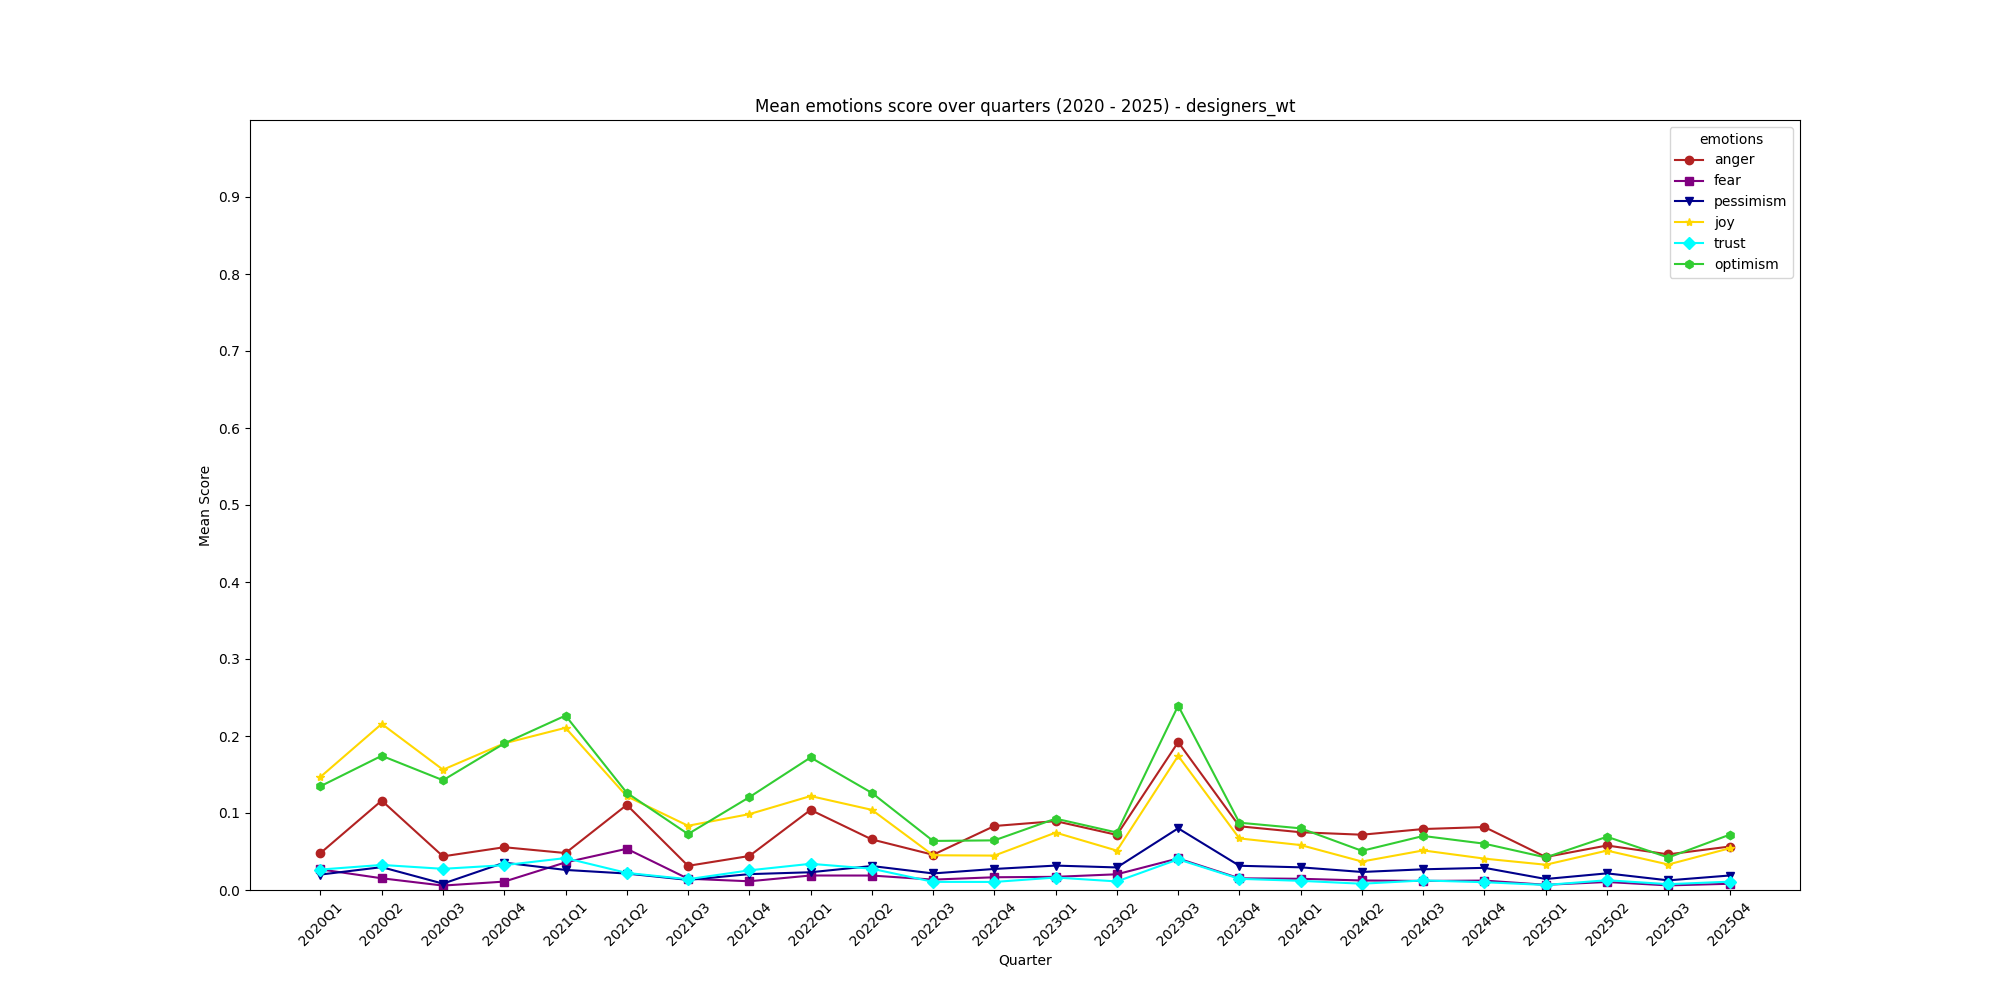
\includegraphics[width=0.95\linewidth]{Images/designers_wt_emotions.png}
    \caption{Weighted emotion mean line graph for the designers' network, with time divided in quarters.}
    \label{fig:des_emotions_wt}
\end{figure}
\begin{figure}[H]
    \centering
    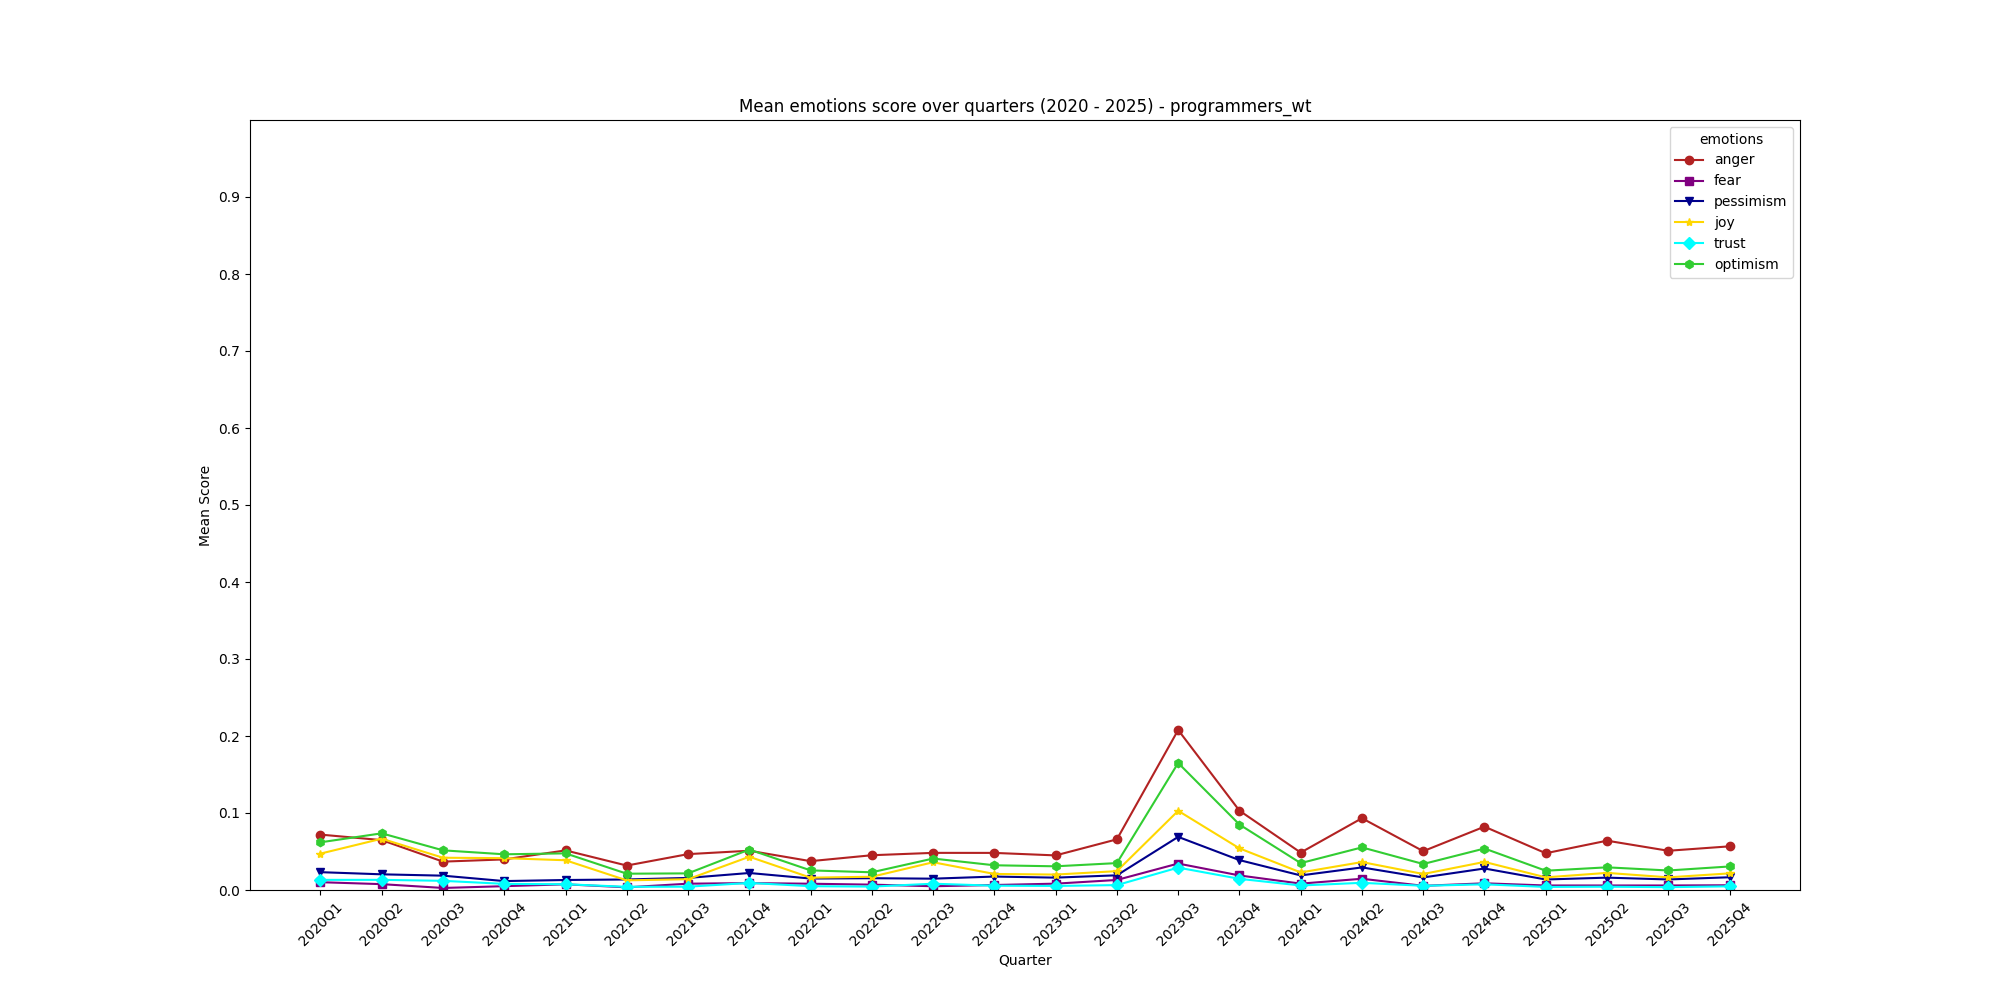
\includegraphics[width=0.95\linewidth]{Images/programmers_wt_emotions.png}
    \caption{Weighted emotion mean line graph for the programmers' network, with time divided in quarters.}
    \label{fig:prog_emotions_wt}
\end{figure}
This results in flatter graphs, which therefore don’t hold much information inside them. The only outlier seems to be in Q3 2023 for both graphs, which is a symptom derived from the fact that the amount of comments for that specific quarter is not statistically significant, as seen in Fig. \ref{fig:number_comments}.

\subsection{Designers}
In the designers' network, the enthusiastic emotions of optimism and joy are consistently two of the highest shown, while trust remains very low across the period. This suggests early excitement about artificial intelligence and generative tools in the workspace. Before the public release of ChatGPT \cite{b24} on November 30, 2022, the prevalent emotions about AI were mostly joy and optimism, although joy slightly declined around the year 2022, possibly because of AI’s scarce notoriety and niche applications. Even though the platform of ChatGPT did not yet allow for image generation, which is the most concerning use of AI for designers, this put a spotlight on all of the other models currently available, such as DALL-E \cite{b25}, released on January 5, 2021, and Midjourney \cite{b26}, released on July 12, 2022, while OpenAI introduced image generation within ChatGPT on March 15, 2025.

On the other hand, the skeptical emotions of fear and pessimism remain consistently low, never overtaking the optimistic emotions overall. However, anger began rising rapidly after 2022 and remains at an elevated level for designers. The gradual rise of anger in the same time period as the decline in joy likely suggests a growing concern about authenticity, labor automation, and more. Nonetheless, overall, designers appear to be more optimistic about AI integration in their work, even after some concerns about trust.
% Image designers emotion
\begin{figure}[H]
    \centering
    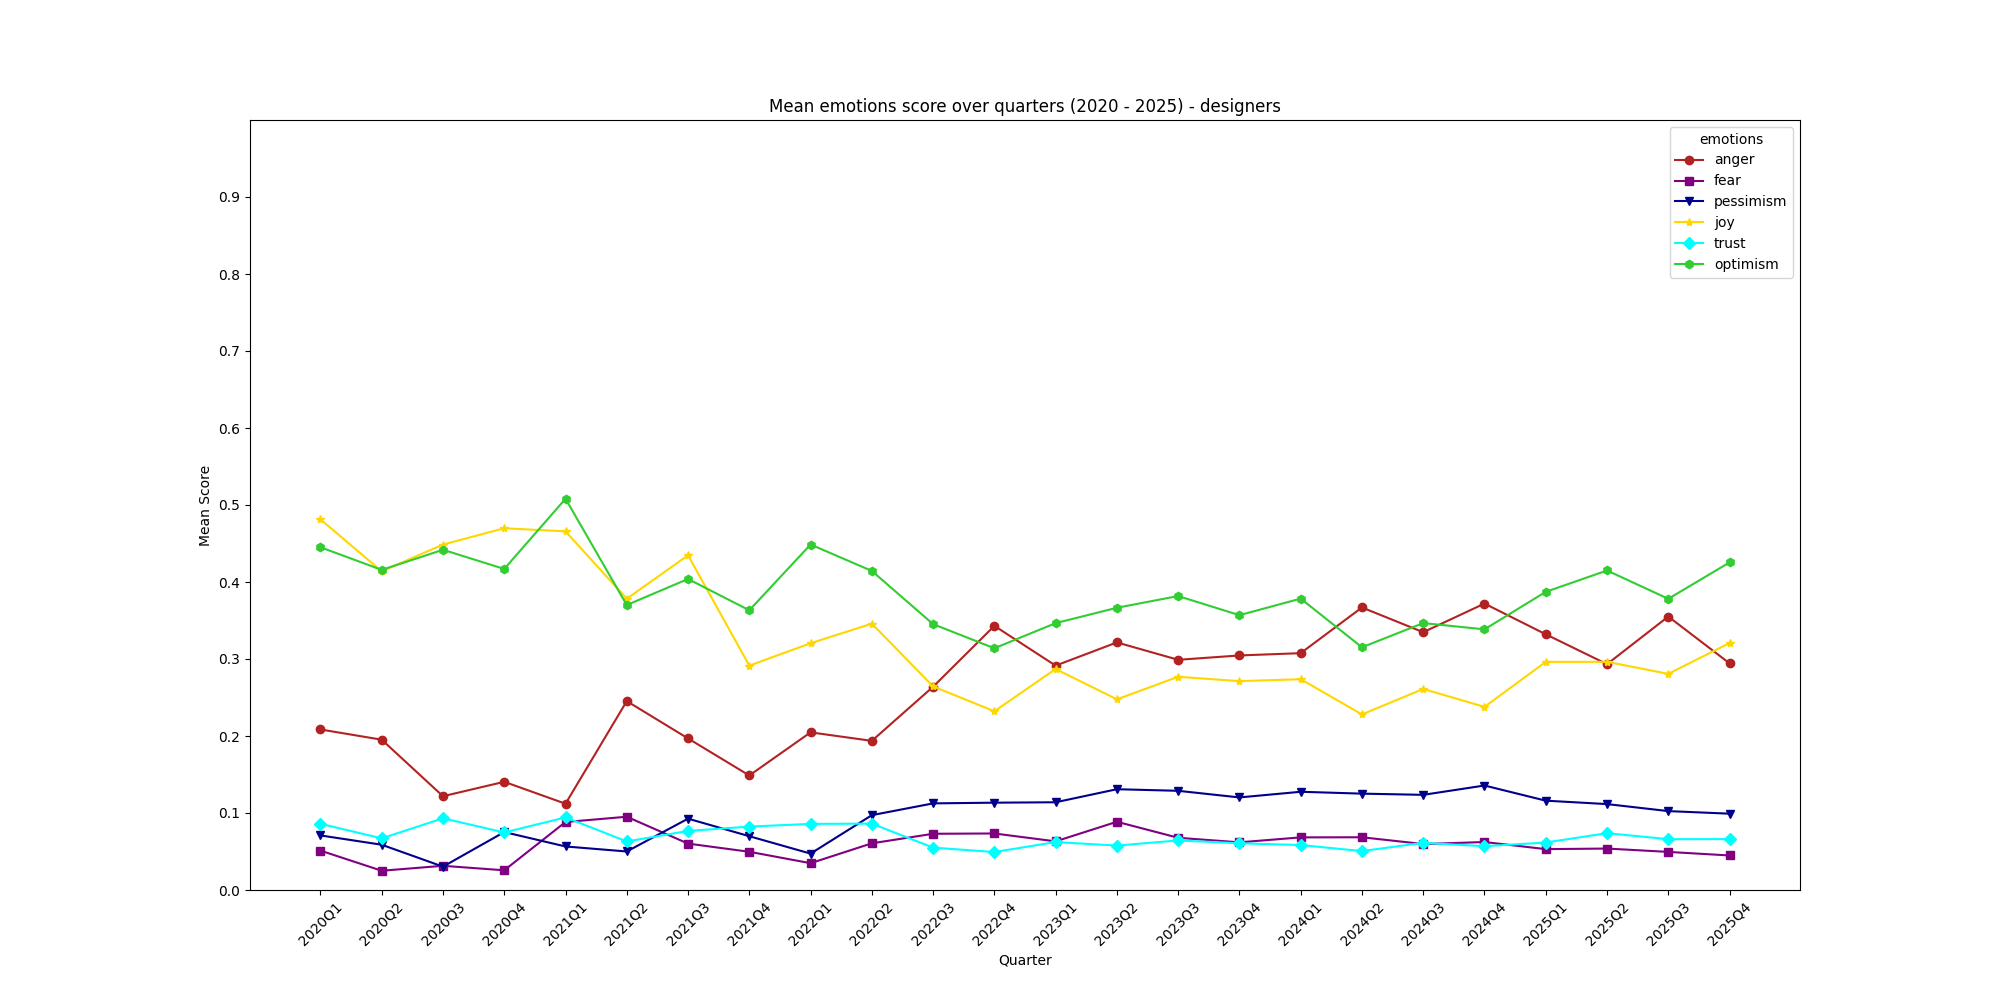
\includegraphics[width=0.95\linewidth]{Images/designers_emotions.png}
    \caption{Emotion mean line graph for the designers' network, with time divided in quarters.}
    \label{fig:des_emotions}
\end{figure}

\subsection{Programmers}
In the programmers' network, even before ChatGPT was released, the dominating emotion was, surprisingly, anger, with a score that was kept high and almost consistent, though steadily increasing. An interesting turning point for anger is in Q2 2023, where the common workplace began using AI to boost performance of developers for a low price, increasing the concerns about workers being replaced by a tool which could, supposedly, allow less expert people to match professionals \cite{b27}. This demonstrates that, even before the popularization of AI in late 2022, programmers already used it for tasks at work. In fact, AI is not simply Large Language Models (LLM), which process natural language after being trained on a vast amount of text, but it has been used for a large variety of tasks, such as recommendation systems, facial recognition, gaming, research, and many more. Moreover, fear and pessimism have a low and consistent score throughout the time frame, supporting the idea that developers may express this more critically.

Conversely, in the enthusiasm spectrum of emotions, similarly to the designers, joy and optimism showcased an initial high score; yet, after 2021, these scores noticeably and subtly started declining as anger continued to rise. Overall, these scores may reflect a more positive emotional reaction, while frustration is mainly reflected and dominant, likely due to critical evaluation such as issues in a forced workplace integration, unreliable responses, system limitations, organizational pressures, and other factors.
% Image programmers emotion
\begin{figure}[H]
    \centering
    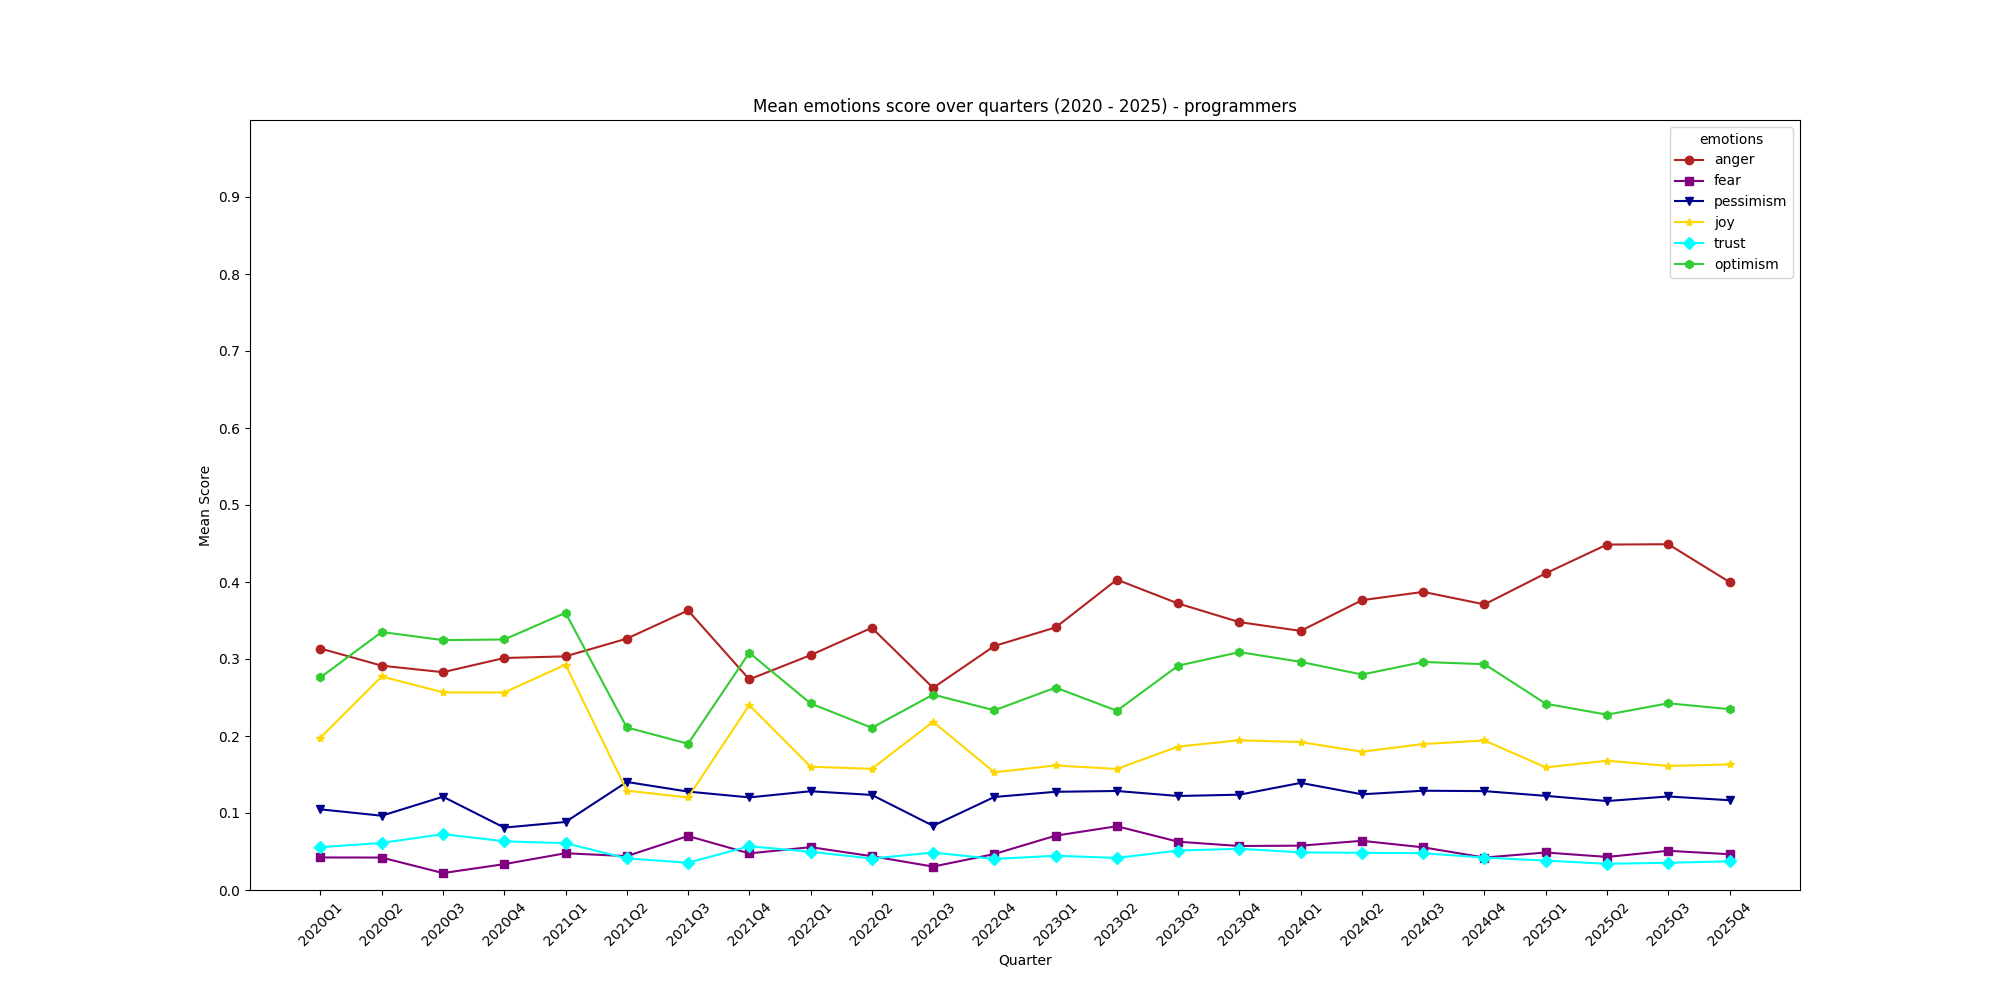
\includegraphics[width=0.95\linewidth]{Images/programmers_emotions.png}
    \caption{Emotion mean line graph for the programmers' network, with time divided in quarters.}
    \label{fig:prog_emotions}
\end{figure}

\subsection{Network-Analytic Interpretation}
When comparing the emotional networks for both designers and developers, data reveals that both communities have diverging reactions to AI integration in their workplace. Although both emotional networks showcase a strong side of optimism and joy, the comparison of their values to other emotions displays a different perspective. In fact, designers maintained a consistent level of optimism and joy even when anger increased, while programmers shifted their perspective drastically towards anger and pessimism when optimism decreased. Therefore, this suggests the opposite emotional response to our hypothesis: designers appear to stand in favor of AI adoption as signs of opportunity with slight concerns, whereas developers gradually converge against AI integration from a more critical evaluative standpoint. A potential explanation based on the topic analysis for the creative community is the ethical concerns, while in the technical community, operational and structural issues arise.\\

Note: All of the emotions’ graphs for both communities together in the same period are available in the Appendix section. In the same section, all emotions’ plots regarding topics are included, apart from the BERTopic ones, of which only the 9 biggest topics’ emotions are shown for the programmers, of which there were 64. You can notice that some of the topics’ emotions graphs are missing data points: that is because, for those specific quarters, there weren’t any comments related to that topic.

\section{Sentiment Analysis (Kristina \& Alessandra)}
To evaluate sentiment, a pre-trained RoBERTa-based deep learning architecture was used. Reddit comments were processed via an automated tokenizer, restricted to a maximum sequence length of 512 tokens with truncation applied where necessary. The individual comments were passed through the model to generate probability scores across three categories: positive, neutral, and negative. These were then synthesized into a single sentiment score:
\begin{align*}
    \text{score}_i = \text{positive}_i(+1) + \text{neutral}_i(0) + \text{negative}_i(-1)
\end{align*}
Importantly, this score reflects the weighted contribution of all three categories, not just the class with the highest probability, providing a more refined measure of sentiment for subsequent analysis.

\subsection{Comment-level analysis}
To examine the relationship between sentiment and community engagement, a correlation analysis was performed between comments and upvotes at the individual comment level. The results showed a negligible negative correlation across both groups ($r=-0.03$), indicating that sentiment polarity does not significantly influence a comment's popularity at the individual level.

From this observation we can draw the conclusion that Reddit, at least as far as the communities analysed are concerned, does not show a tendency to positivity bias, meaning the tendency to make positive messages gain more visibility, which can often be found in more standard social networks, such as Instagram and TikTok. The correlation close to zero indicates, in fact, that users interact with publications not on an emotional basis, nor considering the emotional tone of the creator's comment, but basing their opinion on objective criteria related to the content, its usefulness and its technical value. These are, therefore, communities where the main objective is the exchange of skills.

\subsection{Quarterly temporal aggregation} \label{sec:quarterlyTemporalAggregation}
In order to better understand sentiment evolution, scores were aggregated into quarterly intervals and visualized using bar and line plots. This temporal aggregation served to reduce the noise inherent in individual comments and highlight long-term trends:
\begin{align*}
    \text{score}_q = \frac{1}{N_q} \sum_{i \in q} (p_i^+ - p_i^-)
\end{align*}
Throughout the observation period, both communities maintained a stable sentiment distribution, with only minor fluctuations, as the small range shows. In the unweighted sentiment analysis in Fig. \ref{fig:mean_sentiment} (based on the score formula above), designers exhibit predominantly positive sentiment initially, shifting toward negative values later, coinciding with the announcement of DALL-E and Midjourney, while programmers’ sentiment remains negative throughout.
\begin{figure}[H]
    \centering
    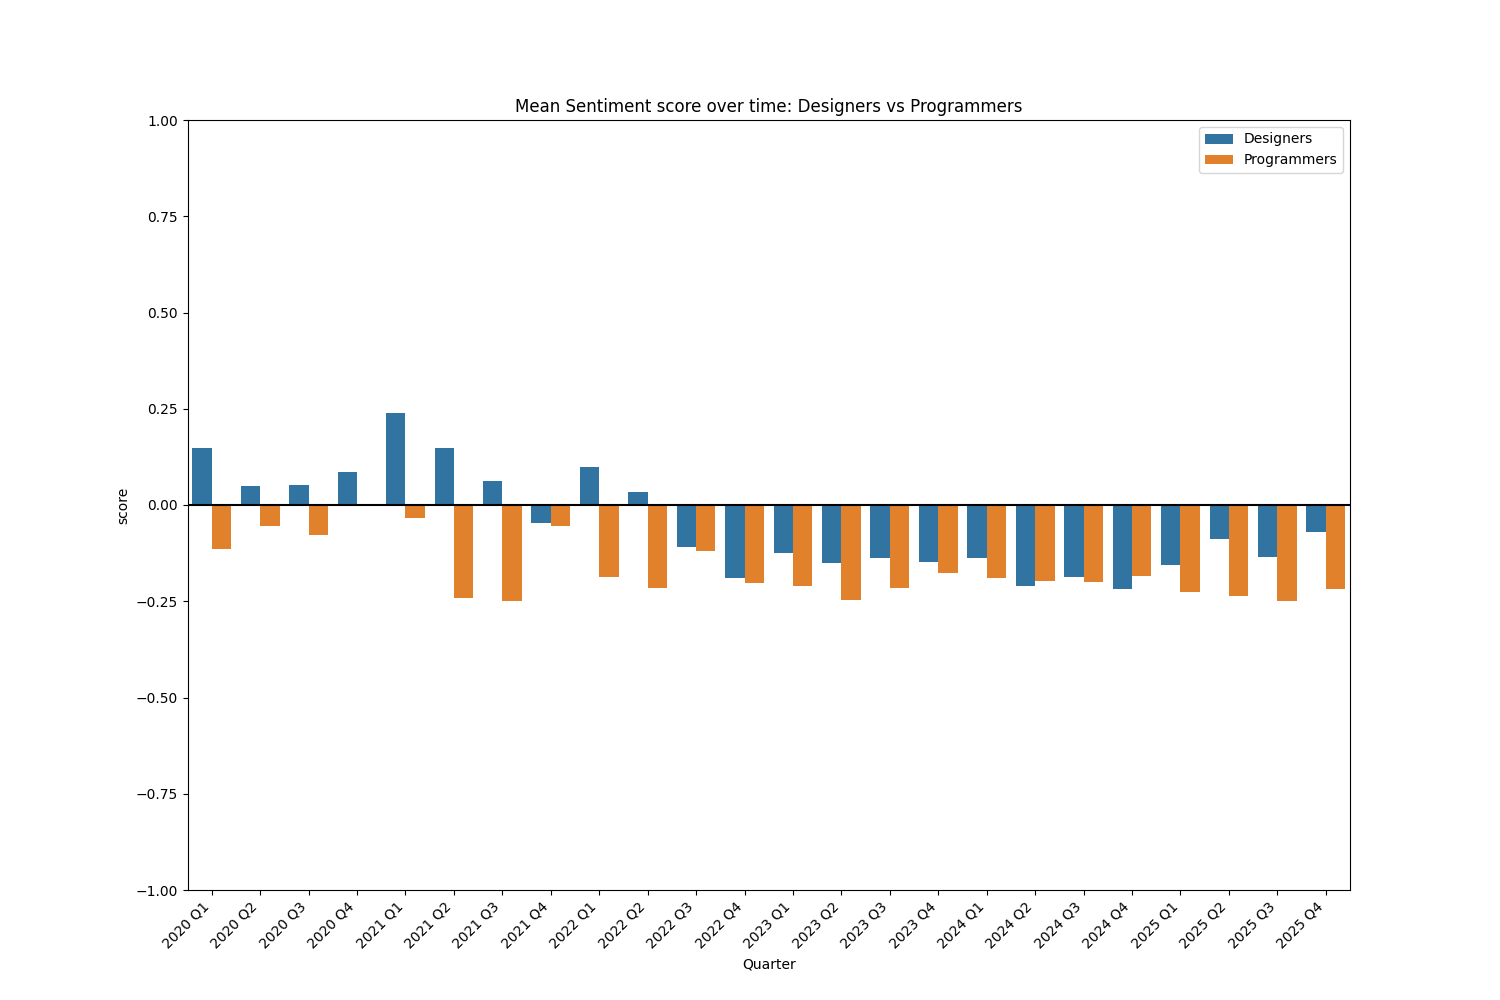
\includegraphics[width=0.95\linewidth]{Images/mean_sentiment_Designers_and_Programmers_over_time.png}
    \caption{Mean sentiment score over time, comparing both the designers' and programmers' networks.}
    \label{fig:mean_sentiment}
\end{figure}
In contrast to the comment-level results, this analysis revealed a moderate negative correlation, particularly within the designers' community. Respectively for the designers and programmers, the correlations are $r = -0.557$ and $r = -0.304$. This divergence highlights the importance of multi-level analysis, as aggregate trends can reveal dynamics that remain obscured at the micro (individual comment) level. For designers, quarters with more upvotes tend to coincide with slightly more negative mean sentiment, suggesting that intense discussions are associated with more critical commentary. On the other hand, the programmers’ sentiment is more stable.

We also analyzed how positive and negative moods interact in each community. In the designers’ community, there is a very strong inverse relationship ($r = -0.902$), suggesting a strongly contrasting sentiment pattern, with swings between positive and negative poles.

In contrast, the programmers show a weaker relationship ($r = -0.713$), reflecting limited positive fluctuations, suggesting a predominantly critical and steady discussion.

From the graph we can see that the sentiment of programmers is more constant over time than that of designers. In the second community mentioned, a big change is noticeable with the advent of DALL-E and Midjourney. This divergence could be explained by considering two different types of social structure and different degrees of homophily. In fact, designers perceived the new artificial intelligence systems as a great threat to their careers, shared by the entire group and which therefore made it united. On the contrary, programmers have demonstrated critical stability to these technological innovations, maintaining the previous sentiment, without being shaken by them.

\subsection{Activity analysis}
The data reveals a consistent upward trend in activity for both designers and programmers. This growth indicates that these discussion networks are expanding and becoming more dense, except for the second half of 2023 which may be associated with the 2023 API controversy, which affects the volume and structure of interaction, creating a temporary slowdown. As the volume of interactions increases, the community environment becomes more complex, amplifying both user engagement and affective fluctuation \cite{b28}.

\subsection{Weighted sentiment analysis}
To account for the influence of more popular comments, we computed a weighted sentiment score for each quarter, multiplying each sentiment class by the log-transformed number of upvotes. This approach ensures that highly upvoted comments influence the mean sentiment while minimizing the impact of extreme outliers.\\
Specifically, the log-transformation is defined as:
\begin{align*}
    w_i = \log(1 + |u_i|)
\end{align*}
The final weighted sentiment score per quarter is computed as:
\begin{align*}
    \text{score}_q = \frac{\sum_{i \in q} [\log(1 + |u_i|)(p_i^+ - p_i^-)]}{\sum_{i \in q} \log(1 + |u_i|)}
\end{align*}
which reflects the average sentiment while giving more weight to comments that received higher engagement.\\

Highly upvoted comments are likely to occupy important positions in the network and therefore have a greater impact on collective sentiment. Aggregating the weighted sentiment quarterly allows us to capture how influential comments shape the overall emotional tone over time, rather than treating all comments equally. This method also enables comparison across communities, highlighting whether designers or programmers have sentiment dynamics that are strongly driven by popular opinions.

When considering the weighted sentiment analysis, the overall temporal pattern remains similar to the unweighted results for both communities. However, a notable exception emerges for the programmers’ community, where a single positive peak appears in the weighted sentiment score.

This discrepancy suggests that during that specific period, a small number of highly upvoted comments expressed a markedly positive sentiment. While these comments did not significantly affect the unweighted mean, their high level of engagement caused them to dominate the weighted measure. The analysis of these positive peaks, relating to the community of programmers, may reveal the presence of some opinion leaders. These are individuals considered important from a social point of view, who, despite the underlying sentiment remaining negative, managed to influence collective perception. This means that a few actors, if popular enough, are able to influence the masses.

In contrast, the close alignment between weighted and unweighted trends in the remaining periods, as well as within the designers’ community, indicates that highly popular comments tend to mirror the overall sentiment of the network.
\begin{figure}[H]
    \centering
    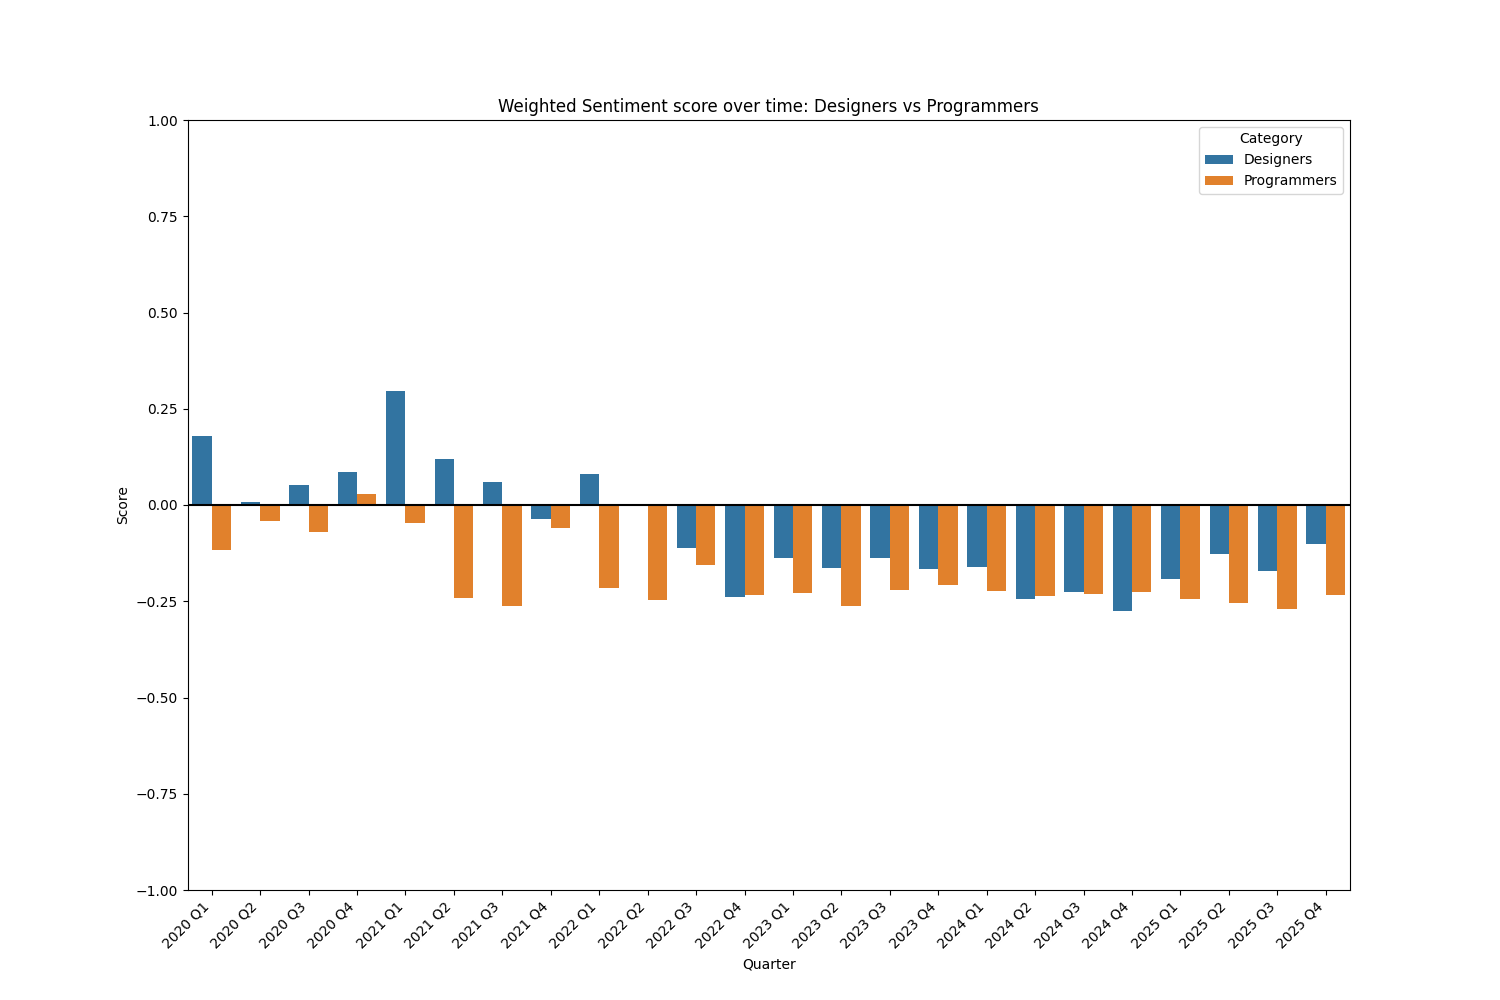
\includegraphics[width=0.95\linewidth]{Images/designers_vs_programmers_weighted_sentiment_over_time.png}
    \caption{Weighted mean sentiment score over time, comparing both the designers' and programmers' networks.}
    \label{fig:mean_sentiment_wt}
\end{figure}
Once again, for designers the correlation was moderately negative ($r= -0.590$) indicating that highly upvoted comments tend to slightly correspond to more negative sentiment, smoothing the observed trend. For programmers, the correlation was weaker ($r = -0.490$), suggesting that negative comments tend to receive slightly more upvotes, but the effect is not that noticeable.

Table \ref{tab:quart_mean_sentiment} summarises the correlations of the quarterly mean sentiments, distinguishing between unweighted and weighted scores, calling attention to the effect of weighting by the log-transformed upvotes.
\begin{table}[H]
    \centering
    \caption{Quarterly mean sentiment}
    \label{tab:quart_mean_sentiment}
    \begin{tabular}{l c c c c c c}
        \hline
        Community & Unweighted corr. & Weighted corr. \\
        \hline
        Designers & -0.557 & -0.590 \\
        Programmers & -0.304 & -0.490 \\
        \hline
    \end{tabular}
\end{table}

\subsection{Year analysis}
To capture how community sentiment evolves across years, the average probabilities of negative, neutral, and positive comments were computed and plotted for each year. In addition, an aggregate sentiment score is computed, summarizing the overall sentiment per year, though this numeric score is not displayed in the barplots. The formula for the aggregate score is:
\begin{align*}
    \text{score} = \frac{1}{N_y} \sum_{i \in y} (p_i^+ - p_i^-)
\end{align*}
In the programmers’ community, as seen in Fig. \ref{fig:prog_year_sentiment}, neutral sentiment consistently represents the largest category throughout the study. Although neutral has the highest probability on average, comments with negative sentiment marginally outweigh the ones with positive, causing the aggregate sentiment to trend slightly negative.

In the designers' community, as seen in Fig. \ref{fig:des_year_sentiment}, neutral sentiment also predominates; however, the early years (2020–2021) reveal a distinct trend where positivity outweighs negativity, indicating an initially supportive environment, again coincident with the only announcement of AI Image generator apps. This dynamic shifts in subsequent years, as negative sentiment increases and eventually surpasses positive probabilities, causing the designers’ profile to converge with the more critical tone seen among programmers.
\begin{figure}[H]
    \centering
    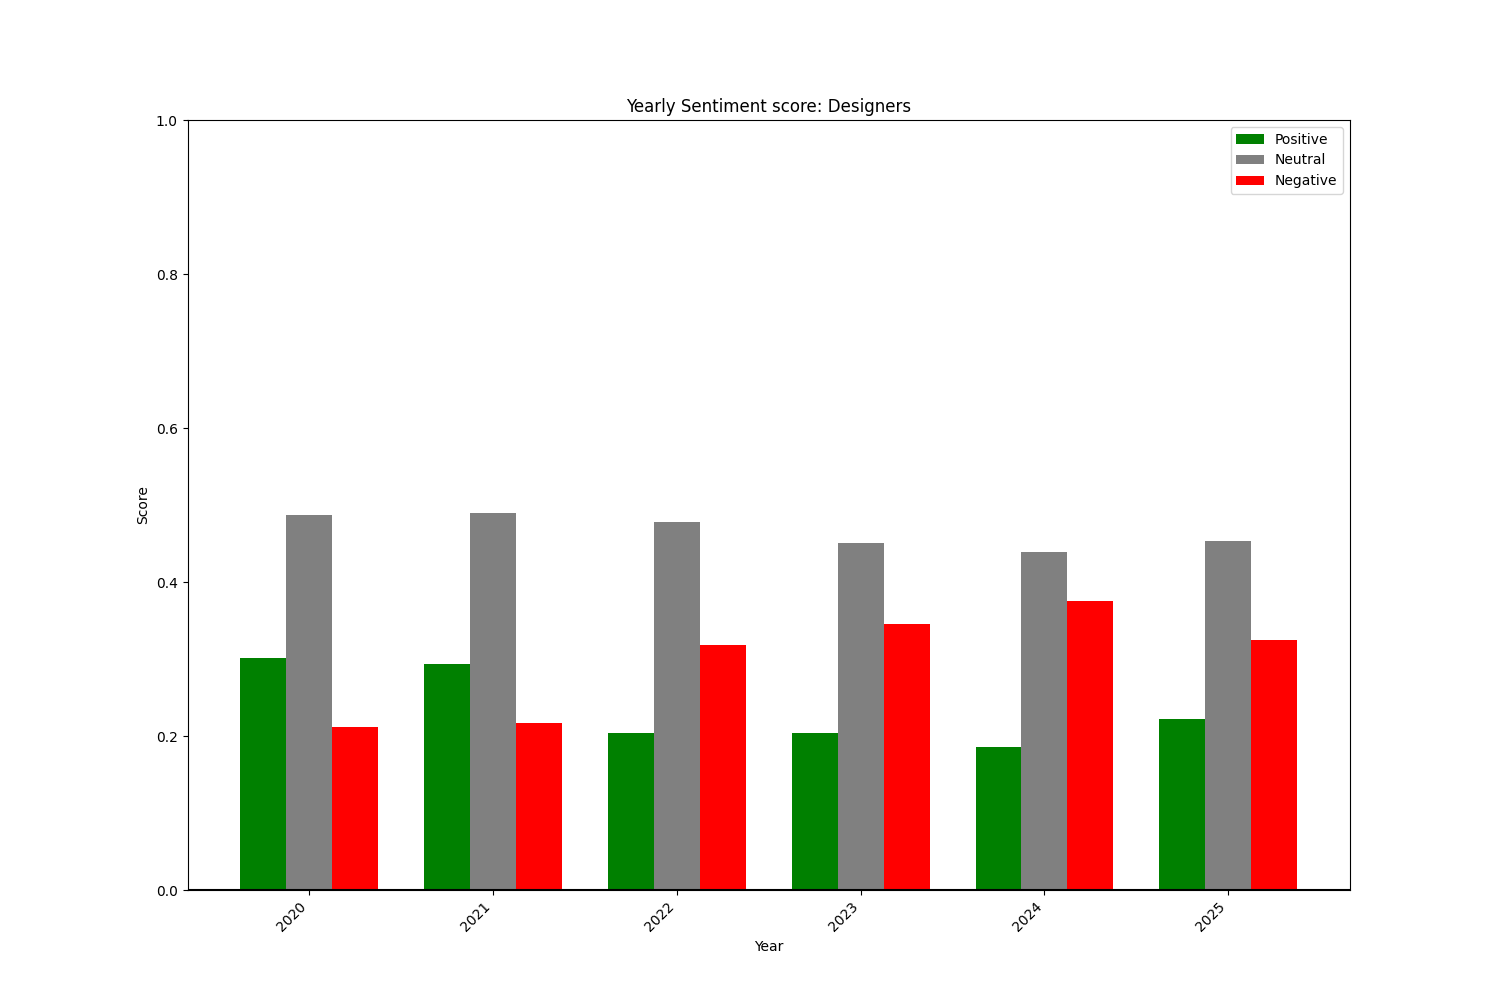
\includegraphics[width=0.95\linewidth]{Images/designers_yearly_sentiment.png}
    \caption{Yearly sentiment score for the designers' network.}
    \label{fig:des_year_sentiment}
\end{figure}
\begin{figure}[H]
    \centering
    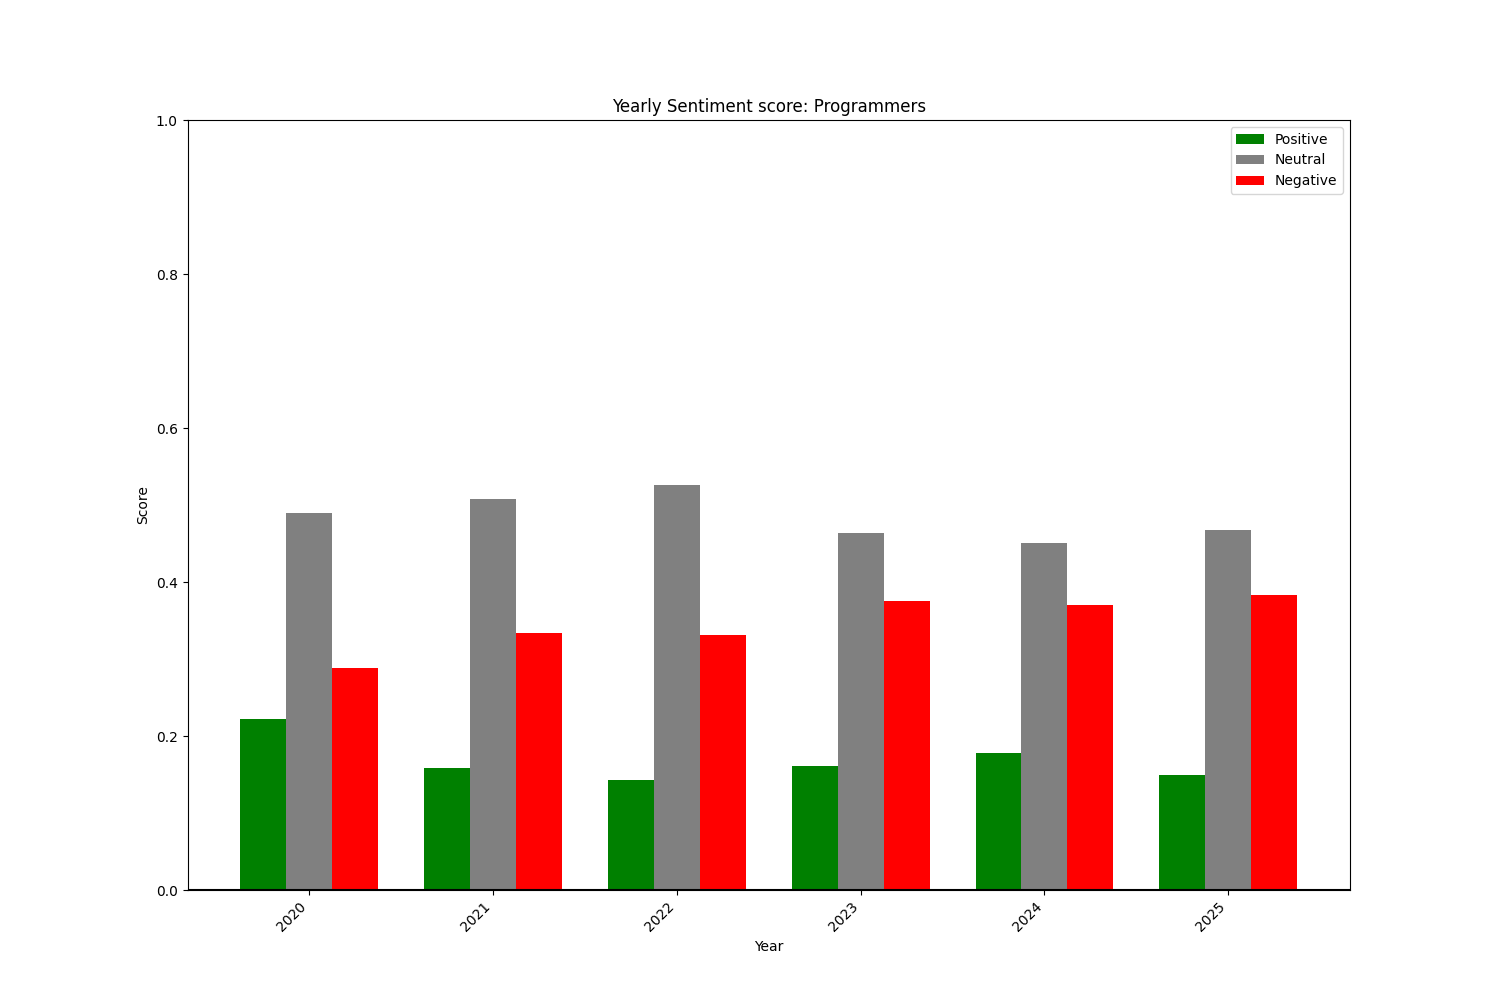
\includegraphics[width=0.95\linewidth]{Images/programmers_yearly_sentiment.png}
    \caption{Yearly sentiment score for the programmers' network.}
    \label{fig:prog_year_sentiment}
\end{figure}

\subsection{Linear regression}
A scatter plot with the regression line was generated to illustrate the relationship. Each point represents a quarterly observation. In this analysis, positive sentiment is treated as the independent variable to examine how changes in positivity relate to changes in negative sentiment.

In the designers’ community, the regression shows a clear negative slope, indicating that periods of high weighted positivity are generally accompanied by a decrease in weighted negativity. The sentiment values span a wide range from positive to negative, suggesting that the network tends to align around a single dominant feeling, transitioning from very positive to more negative periods.

In contrast, the programmers also exhibit a negative trend, but it seems to be less pronounced. Their positive sentiment values are concentrated in a lower range, while negative sentiment values are generally higher. The points are more clustered, indicating that the community typically exhibits more negative sentiment and a narrower variation overall. While highly upvoted comments still influence the overall mood, the network does not shift dramatically toward extreme positivity, and even when influential comments are strongly positive, a baseline of negativity persists. This indicates that popular opinions guide discussion, but the programmers’ community largely remains within a negative or low-sentiment range.
\begin{figure}[H]
    \centering
    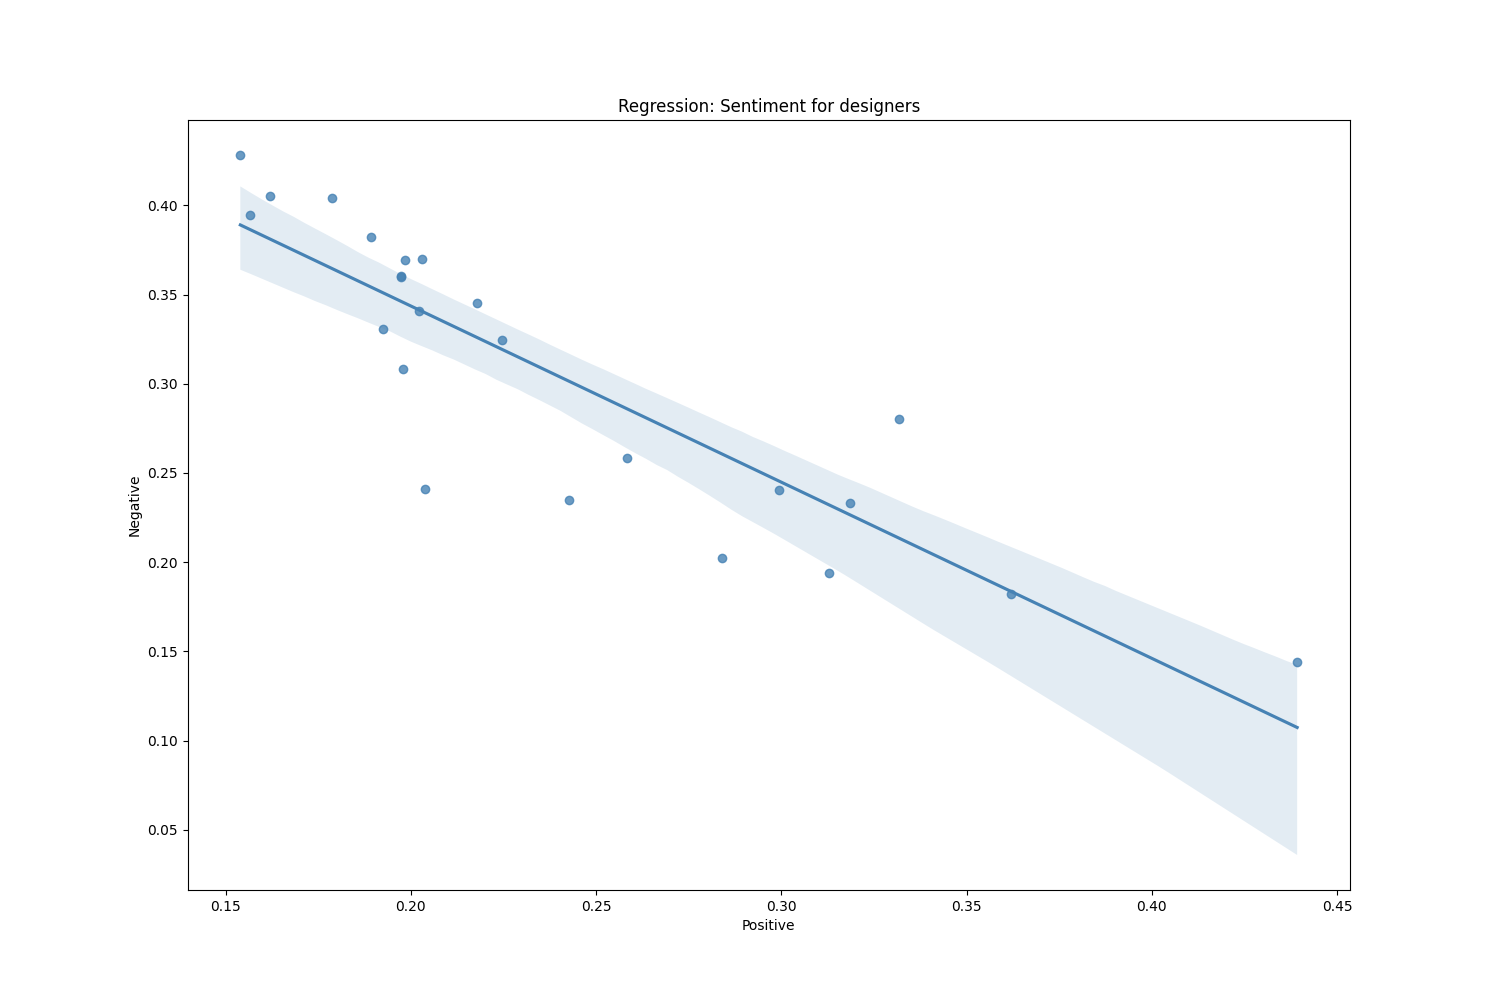
\includegraphics[width=0.95\linewidth]{Images/designers_regression.png}
    \caption{Regression on sentiment for the designers' network.}
    \label{fig:des_sentiment_regression}
\end{figure}
\begin{figure}[H]
    \centering
    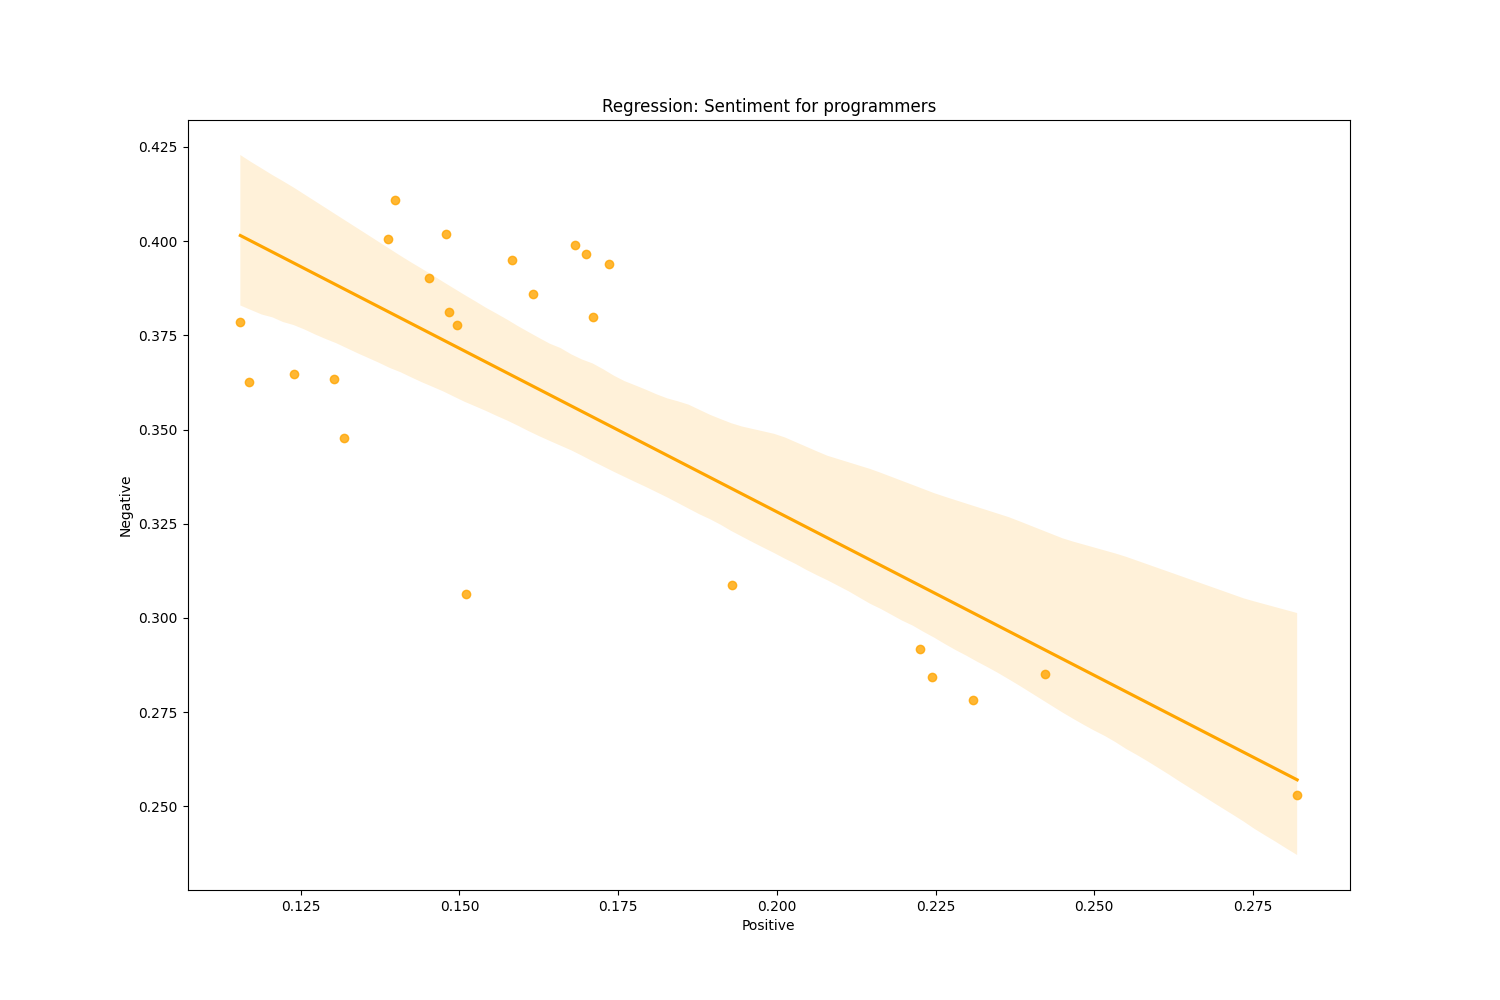
\includegraphics[width=0.95\linewidth]{Images/programmers_regression.png}
    \caption{Regression on sentiment for the programmers' network.}
    \label{fig:prog_sentiment_regression}
\end{figure}
Consistent with what is expressed in section \ref{sec:quarterlyTemporalAggregation}, it is still possible to see that the community of designers and that of programmers present a great structural difference. The former, in fact, is characterized by high cohesion, which leads to the conformity of the group and, therefore, to align on the same dominant sentiment. At the same time, developers prove to be more consistent and their sentiment is quite independent of upvotes.

Note: In the appendix, all plots for the designers are provided, including results from both BERTopic and Louvain, whereas for the programmers, all Louvain plots are included, but only the first nine BERTopic plots are shown. Consistent with the analyses presented in this section, the appendix displays only the weighted sentiment results, even though both unweighted and weighted scores were computed. The differences between weighted and unweighted plots are most pronounced when focusing on the narrow sentiment range around -0.25 to 0.25. In this range, small variations in comment popularity can shift the score from slightly positive to slightly negative (or vice versa).

It is important to note that dots with a score of zero do not indicate neutral sentiment; rather, they correspond to quarters in which specific topics were absent or not discussed. Consequently, line plots may show extended periods with a score of zero, reflecting gaps in thematic discussion rather than actual neutrality.

\section{Semantic Networks (Kristina \& Alessandra)}

The aim of this study is to map and compare the conceptual structures of two distinct professional communities by reconstructing semantic networks through Gephi. The objective is to move beyond simple word-frequency analysis and uncover the latent semantic relationships that shape professional discourse and identity in digital communities.

The analysis, based on the construction of a weighted word to word adjacency network, is derived from the probabilistic projection of a document to word matrix. Words are linked according to their shared probability distributions across the document set, not merely on their co-occurrence within a sentence or short textual window.

Despite the high density and unstructured nature of Reddit data, which often lacks the data found on platforms like X, the application of PageRank and modularity allows for a clear structural breakdown. To ensure the interpretability of the results and reduce noise, a degree-based filtering was applied, pruning the network to a core of approximately 500 nodes. This selection focuses on the most significant terms in order to achieve a robust application of the following measures:
\begin{itemize}
    \item PageRank: used to determine the hierarchy, highlighting influential words based on both their number of connections and the importance to which they are connected;
    \item Louvain: community detection was performed by optimizing modularity and assigning each node to a modularity class.
\end{itemize}
Louvain was applied to the weighted word to word network to partition the network into internally coherent communities: it identifies groups of words that are more tightly linked to each other than to the rest of the network. The resulting color-coded clusters represent thematic communities, showing groups of words that share similar semantic distributions across documents.

Two configurations were considered: the default resolution parameter and an adjusted version of it, in order to evaluate how the scale of community detection influences the structure of the networks. Increasing the resolution leads to fewer larger communities and to a higher modularity score for both groups, suggesting that the discussion is organized around macro conceptual domains rather than micro-topics.
\begin{table}[H]
    \centering
    \caption{Quarterly mean sentiment}
    \label{tab:quarter_mean_sentiment}
    \begin{tabular}{l c c c c c c}
        \hline
        & Modularity (default) $\gamma = 1.0$ & Modularity (adjusted $\gamma$) \\
        \hline
        Designers & 0.239 & 0.312 ($\gamma = 1.2$) \\
        Programmers & 0.244 & 0.281 ($\gamma = 1.1$) \\
        \hline
    \end{tabular}
\end{table}
Following community detection, the networks were spatialized using the ForceAtlas2 layout in Gephi and, due to the extreme density, the scaling factor was increased and the strong gravity option was enabled. This way, the repulsion between nodes is amplified, creating a more interpretable spatial distribution and preventing peripheral nodes from drifting excessively away from the main structure.

PageRank was explicitly used to determine the text size of nodes in the visualization: words with higher PageRank values are shown larger, making their importance immediately visible. In this way, a word is considered important not only if it has many connections, but if it is connected to other important words.

This analysis is subject to limitations inherent to Reddit data, leading to highly noisy graphs characterized by elevated average degree values, which require strong algorithmic filtering to extract meaningful structure. 

\subsection{Designers}

Concerning the designers, both Degree and PageRank produce a similar ranking of words, indicating that highly connected words are also influential within the network. Interestingly, the top-ranked words according to PageRank all have a high eccentricity, suggesting that these influential words are centrally positioned relative to the rest of the network. Similarly, closeness centrality and harmonic closeness are very high, confirming that they can efficiently reach other nodes. Betweenness, on the other side, is extremely low across all nodes, indicating that shortest paths are rarely mediated by any single word. Finally, weighted degree mirrors PageRank for the top-ranked words, highlighting that both the strength and number of connections contribute to a word’s importance in the network. The top-ranked words are highly central and influential, while the others are peripheral, with limited connectivity and reach.

Table \ref{tab:des_semantic_topics} represents an attempt to identify general topics for each cluster. Although carefully determined, they are not exhaustive, given the quantity and variety of words that most clusters present. However, this operation allows for an overview of the salient macrotopics in the semantic networks created.
\begin{table}[h]
    \centering
    \caption{Designers' general topics for each cluster}
    \label{tab:des_semantic_topics}
    \begin{tabular}{p{1cm} p{0.5cm} p{2cm} p{3cm}}
        \hline
        Modularity class & \% & General topic & Keywords \\ \hline
        \cellcolor[HTML]{119083} 0 & 21,73 & Asset management and ownership & Copyright, benefit, asset \\ \hline
        \cellcolor[HTML]{6aa84f} 1 & 12,68 & User experience & Easy, clear, experience \\ \hline
        \cellcolor[HTML]{059763} 2 & 8,65 & AI as a creative aid & AI, reference, template \\ \hline
        \cellcolor[HTML]{ff00ff} 3 & 14,89 & Professional practice & Edit, profession, portfolio \\ \hline
        \cellcolor[HTML]{f5199a} 4 & 9,05 & Market-driven creation & Artwork, customer, product \\ \hline
        \cellcolor[HTML]{b45f06} 5 & 5,43 & Learning and experimental process & Luck, try, understand \\ \hline
        \cellcolor[HTML]{12abff} 6 & 5,23 & Industry evolution & Shift, old, role \\ \hline
        \cellcolor[HTML]{ff0000} 7 & 15,9 & Job seeking & Logo, employer, interview \\ \hline
        \cellcolor[HTML]{6b90ca} 8 & 6,44 & Client solutions & Client, impact, solution \\ \hline
    \end{tabular}
\end{table}
\begin{figure}[h]
    \centering
    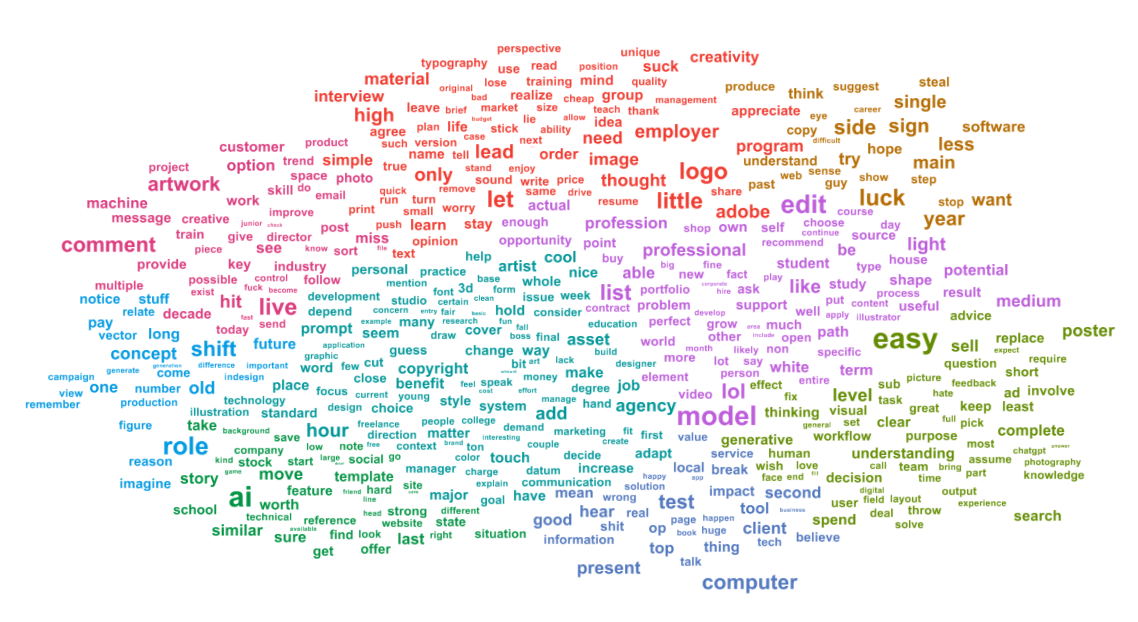
\includegraphics[width=0.95\linewidth]{Images/designers_visualization_screenshot.png}
    \caption{Designers word network with clusters.}
    \label{fig:des_word_network}
\end{figure}
The semantic network of designers, therefore, presents itself as a compact group. The strong overlap between Degree and PageRank values indicates that the most frequent words are also the most important, which means that there is a central core of shared ideas. Analyzing the lexicon in detail, it can be observed that this community tends to respond to the integration of AI into its work mainly from the point of view of the quality of the experience: this is evidenced by terms such as \textit{easy}, \textit{luck}, \textit{feel}, \textit{good} and \textit{cool}. In addition, it is noticeable that, in order to evaluate them and be able to express a global opinion about them, new technologies are immediately included in their workflow: in fact, we find terms such as \textit{edit}, \textit{logo}, \textit{template}, \textit{reference} and \textit{product}.

\subsection{Programmers}
The network analysis reveals distinct roles for nodes based on different measures. PageRank identifies the most influential nodes, which occupy central positions in terms of connections and visibility. High-degree nodes, in contrast, often correspond to frequently occurring words (e.g., \textit{be}, \textit{have}, \textit{do}, \textit{use}, \textit{make}, \textit{get}). Weighted degree aligns closely with PageRank, suggesting that influence emerges from both the number and strength of connections.

Closeness centrality and harmonic closeness indicate that top-ranked nodes can efficiently reach other nodes, whereas lower-ranked nodes are distant and poorly connected. Betweenness centrality, which quantifies the extent to which a node lies on shortest paths between others, is uniformly low across the network, reflecting its dense connectivity and suggesting that influence arises primarily from direct relationships rather than intermediary bridging roles.

Eccentricity provides additional structural insight. While low eccentricity typically characterizes centrally located nodes, our results show that nodes with high PageRank also exhibit relatively high eccentricity. This indicates that, although these nodes are locally influential, they remain distant from certain peripheral regions of the network, highlighting a divergence between local influence and global centrality.

Table \ref{tab:prog_semantic_topics} represents an attempt to identify general topics for each cluster. Although carefully determined, they are not exhaustive, given the quantity and variety of words that most clusters present. However, this operation allows for an overview of the salient macrotopics in the semantic networks created.

\begin{table}[H]
    \centering
    \caption{General topics for each cluster}
    \label{tab:prog_semantic_topics}
    \begin{tabular}{p{1cm} p{0.5cm} p{2cm} p{3cm}}
        \hline
        Modularity class & \% & General topic & Keywords \\ \hline
        \cellcolor[HTML]{129b81} 0 & 4,24 & Corporate systems & Model, company, network \\ \hline
        \cellcolor[HTML]{a09ab4} 1 & 1,35 & Development timeframes & Week, long, window \\ \hline
        \cellcolor[HTML]{ff0000} 2 & 10,98 & Legal documentation & Software, license, documentation \\ \hline
        \cellcolor[HTML]{e69138} 3 & 6,55 & Professional development & Grow, improve, offer \\ \hline
        \cellcolor[HTML]{f5199a} 4 & 9,83 & AI as a resource & Llm, solution, resource \\ \hline
        \cellcolor[HTML]{c03bce} 5 & 12,91 & Operations and scaling & Scale, method, management \\ \hline
        \cellcolor[HTML]{6aa84f} 6 & 3,85 & AI versions & Modern, review, version \\ \hline
        \cellcolor[HTML]{12abff} 7 & 5,01 & Personal growth & Life, personal, learning \\ \hline
        \cellcolor[HTML]{1111b1} 8 & 10,6 & Comparative analysis & Compare, describe, realize \\ \hline
        \cellcolor[HTML]{b45f06} 9 & 3,85 & Emerging AI platforms & Actual, openai, copilot \\ \hline
        \cellcolor[HTML]{12c25e} 10 & 30,83 & Technical clarity & Clear, library, framework \\ \hline
    \end{tabular}
\end{table}
\begin{figure}[H]
    \centering
    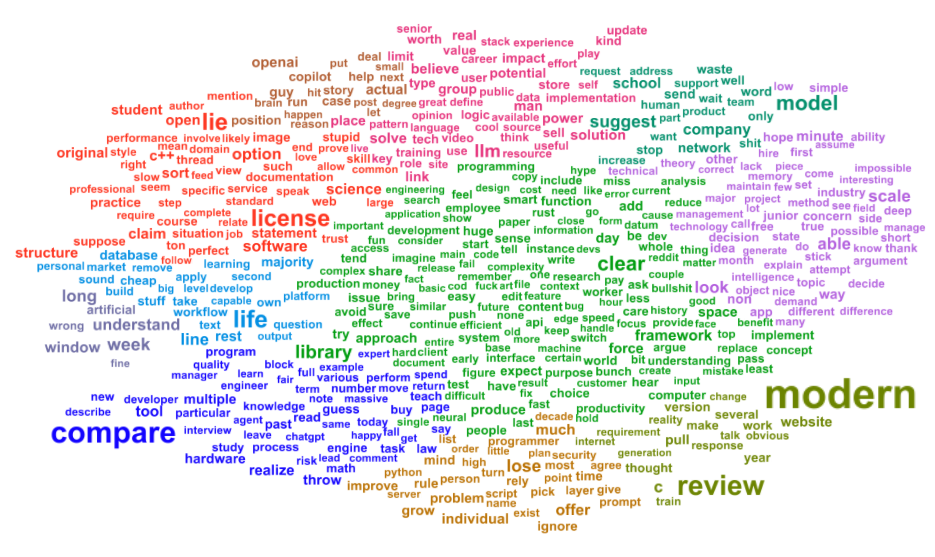
\includegraphics[width=0.95\linewidth]{Images/programmers_visualization_screenshot.png}
    \caption{Programmers word network with clusters}
    \label{fig:prog_word_network}
\end{figure}
This network is characterized by a more fragmented structure and it is divided into distinct technical sectors. From keywords such as \textit{license}, \textit{compare}, \textit{review}, \textit{tool} and \textit{result}, it is possible to deduce that the language used is mainly aimed at technical analysis. An analytical process, based on verification, precision and legality, can be identified. It is, consequently, a pragmatic approach, which allows the issue to be discussed in a mostly objective way, verifying its performance.

\subsection{Comparison between the two networks}
The comparison between the two semantic networks highlights the presence of two different professional cultures between the two communities, which depend on the fundamental characteristics of the respective profession. Designers, in fact, demonstrate a targeted attention to the experience of using AI and aesthetics, and therefore to evaluations that are still subjective, but mostly shared within the group. This is consistent with their profession, since personal taste, ease of use of a product, artistic sensitivity and attention to the user are essential characteristics.

On the contrary, programmers demonstrate a mentality based more on purely technical and legal aspects. This demonstrates a more logical approach, characterized by analytical rigor, being not very attentive to emotions, but above all by technical competence. It is a network that is not characterized by a well-defined central core, but a structure characterized by specialisations, even if consistent with each other: the different subgroups show specific technical languages, from the focus on comparison, to the focus on legal issues.

\subsection{Final semantic considerations}
In the designers’ network, words such as \textit{ai} and \textit{model} refer to the emerging technologies and application, while \textit{edit} and \textit{logo} reflect some concrete aspects of professional practice. The presence of evaluative terms like \textit{easy} and \textit{luck} incorporates experiential and subjective evaluations, related to personal experience and assessment of tools and outcomes.

In the programmers’ network, words such as \textit{compare} and \textit{review} suggest analytical practices, while \textit{license} draws attention to regulatory and legal considerations. Additionally, \textit{clear} could suggest a focus on unambiguous communication, while \textit{lie} could point to errors and inaccuracies in the code.

The occurrence of \textit{model} in both is significant, as it suggests a shared reference across the two communities. While its centrality likely relates to AI models in both the contexts, the term may carry different specific connotations and applications within each professional domain.
\begin{table}[H]
    \centering
    \caption{Top 8 words according to PageRank}
    \begin{tabular}{l l}
        \hline
        Network & Top words \\
        \hline
        Designers & easy, ai, model, edit, role, live, luck, logo \\
        Programmers & modern, compare, review, life, lie, license, model, clear \\
        \hline
    \end{tabular}
\end{table}

\section{Conclusions (Charlie)}
This study investigated how online professional communities polarize between enthusiasm and skepticism toward Artificial Intelligence integration in work practices, focusing on programmers and designers. By combining Social Network Analysis with topic modeling, emotion analysis, and sentiment analysis, we examined both the structural organization of discussions and the meanings and emotions embedded within them. The results reveal that polarization toward AI is shaped by distinct professional logics.

Programmers’ discourse is predominantly instrumental, clustering around efficiency, coding support, problem solving, and learning. In this community, enthusiasm toward AI is structurally dominant, while skepticism appears in a conditional and technical form, primarily addressing issues of reliability, data use, and legal constraints rather than questioning AI’s legitimacy as a tool. Designers, in contrast, exhibit a more reflexive and evaluative discourse. Their discussions emphasize feedback, originality, portfolios, and professional identity, reflecting deeper concerns about authorship and creative authority. While designers also express enthusiasm, particularly toward experimentation and ideation, skepticism is more embedded within the discourse and tied to fears of skill devaluation and loss of human contribution. Emotion and sentiment analyses support this distinction. Designers show more synchronized emotional shifts over time, indicating stronger collective polarization, where programmers maintain a more mixed emotional environment in which positive and critical evaluations coexist. Engagement metrics such as upvotes display little direct correlation with emotional tone, suggesting that popularity does not straightforwardly amplify enthusiasm or skepticism.

Overall, the findings indicate that attitudes toward AI are not simply individual preferences but are embedded in the semantic priorities and social structures of professional communities. By integrating network and language-based approaches, this study highlights how technological acceptance is negotiated collectively and differently across occupational contexts. These insights contribute to a more nuanced understanding of AI adoption as a socially constructed and professionally mediated process.

\clearpage

\begin{thebibliography}{00}

\bibitem{b1}
F.~D. Davis,
``User acceptance of information technology: system characteristics, user perceptions and behavioral impacts'',
\emph{International Journal of Man-Machine Studies}, vol.~38, no.~3, pp.~475--487, 1993.

\bibitem{b2}
V.~Venkatesh, M.~G. Morris, G.~B. Davis, and F.~D. Davis,
``User acceptance of information technology: toward a unified view'',
\emph{MIS Quarterly}, vol.~27, no.~3, pp.~425--478, 2003.

\bibitem{b3}
T.~J. Pinch and W.~E. Bijker,
``The social construction of facts and artefacts: or how the sociology of science and the sociology of technology might benefit each other'',
\emph{Social Studies of Science}, vol.~14, no.~3, pp.~399--441, 1984.

\bibitem{b4}
P.~D. Koenig,
``Attitudes toward artificial intelligence: combining three theoretical perspectives on technology acceptance'',
\emph{AI \& Society}, vol.~40, no.~3, pp.~1333--1345, 2024.

\bibitem{b5}
R.~Appanagari, I.~Singh, A.~Sule, and S.~Jahanikia,
``Behavioral plasticity in advanced technology adoption: a cognitive dissonance analysis'',
\emph{Journal of Brain Science and Mental Health}, vol.~1, no.~1, pp.~1--15, 2025.

\bibitem{b6}
Q.~Zhang, G.~Liao, X.~Ran, and F.~Wang,
``The impact of AI usage on innovation behavior at work: the moderating role of openness and job complexity'',
\emph{Behavioral Sciences}, vol.~15, no.~4, p.~491, 2025.

\bibitem{b7}
H.~Ahmad, M.~M. Gulzar, I.~Ahmed, and M.~Khalid,
``Adoption of modern digital innovations: a systematic review of social impacts in online community forums'',
\emph{Social Network Analysis and Mining}, vol.~15, p.~29, 2025.

\bibitem{b8}
A.~Grunewald and M.~Kräkel,
``Information manipulation and competition'',
\emph{Games and Economic Behavior}, vol.~131, pp.~245--263, 2022.

\bibitem{b9}
D.~C. Garzón-Velandia, M.~I. Barreto-Galeano, and J.~M. Sabucedo-Cameselle,
``What is polarization in the social sciences? A scoping review of reviews'',
\emph{Acta Colombiana de Psicología}, vol.~27, no.~2, 2024.

\bibitem{b10}
M.~Khemka and B.~Houck,
``Toward effective AI support for developers: A survey of desires and concerns'',
\emph{Communications of the ACM}, vol.~67, no.~11, pp.~42--49, 2024.

\bibitem{b11}
M.~Kalving, A.~Colley, and J.~Häkkilä,
``Where AI and design meet—Designers’ perceptions of AI tools'',
in \emph{Proceedings of the 13th Nordic Conference on Human-Computer Interaction}, 2024, pp.~1--8.

\bibitem{b12}
U.~Wilkens,
``Artificial intelligence in the workplace—A double-edged sword'',
\emph{The International Journal of Information and Learning Technology}, vol.~37, no.~5, pp.~253--265, 2020.

\bibitem{b13}
Watchful1,
``Reddit Submissions from 2005-06 to 2025-06'', Available: \url{https://academictorrents.com/details/30dee5f0406da7a353aff6a8caa2d54fd01f2ca1}

\bibitem{b14}
Watchful1,
``PushshiftDumps github'', Available: \url{https://github.com/Watchful1/PushshiftDumps/tree/master?tab=readme-ov-file}

\bibitem{b15}
M.~Honnibal, I.~Montani, 
``spaCy 2: Natural language understanding with Bloom embeddings, convolutional neural networks and incremental parsing'',
2017.

\bibitem{b16}
M.~Bastian, S.~Heymann, M.~Jacomy,
``Gephi: an open source software for exploring and manipulating networks'',
in \emph{Third international AAAI conference on weblogs and social media}, 2009.

\bibitem{b17}
J.~Alstott, E.~Bullmore, D.~Plenz,
``powerlaw: A Python Package for Analysis of Heavy-Tailed Distributions'',
in \emph{PLoS ONE}, 2014, 9(1), e85777

\bibitem{b18}
A.~A. Hagberg, D.~A. Schult, and P.~J. Swart,
``Exploring network structure, dynamics, and function using NetworkX'',
in \emph{Proceedings of the 7th Python in Science Conference (SciPy2008)},
Pasadena, CA, USA, 2008, pp.~11--15.

\bibitem{b19}
V.~D. Blondel, J.-L. Guillaume, R.~Lambiotte, and E.~Lefebvre,
``Fast unfolding of communities in large networks'',
\emph{Journal of Statistical Mechanics: Theory and Experiment}, vol.~2008, no.~10, p.~P10008, 2008.

\bibitem{b20}
G.~Grootendorst,
``BERTopic: Neural topic modeling with a class-based TF-IDF procedure'',
2022. Available: \url{https://arxiv.org/abs/2203.05794}.

\bibitem{b21}
L.~McInnes, J.~Healy, J.~Melville, 
``UMAP: Uniform Manifold Approximation and Projection for Dimension Reduction'',
2020.

\bibitem{b22}
L.~McInnes, J.~Healy,
``Accelerated Hierarchical Density Based Clustering''. 
in \emph{2017 IEEE International Conference on Data Mining Workshops (ICDMW)}, 
2017, pp. 33–42.

\bibitem{b23}
D.~Antypas, A.~Ushio, F.~Barbieri, L.~Neves, K.~Rezaee,
L.~Espinosa-Anke, J.~Pei, and J.~Camacho-Collados,
``SuperTweetEval: A challenging, unified and heterogeneous benchmark for social media NLP research'',
in \emph{Findings of the Association for Computational Linguistics: EMNLP 2023}, 2023.

\bibitem{b24}
OpenAI,
``ChatGPT'', Available: \url{https://openai.com/index/chatgpt/}.

\bibitem{b25}
OpenAI,
``DALL·E'', Available: \url{https://openai.com/index/dall-e/}.

\bibitem{b26}
Wikipedia,
``MidJourney'', Available: \url{https://en.wikipedia.org/wiki/Midjourney}.

\bibitem{b27}
P.~Cihon,
``How AI-powered software development may affect labor markets'',
2023.
Available: \url{https://www.brookings.edu/articles/how-ai-powered-software-development-may-affect-labor-markets/}

\bibitem{b28}
H.~Field,
``Reddit is in crisis as prominent moderators loudly protest the company’s treatment of developers,''
CNBC, 2023.
Available: \url{https://www.cnbc.com/2023/06/16/reddit-in-crisis-as-prominent-moderators-protest-api-price-increase.html}

\end{thebibliography}

\onecolumn
\appendices
\section{Emotion Analysis}
\begin{figure}[H]
    \centering
    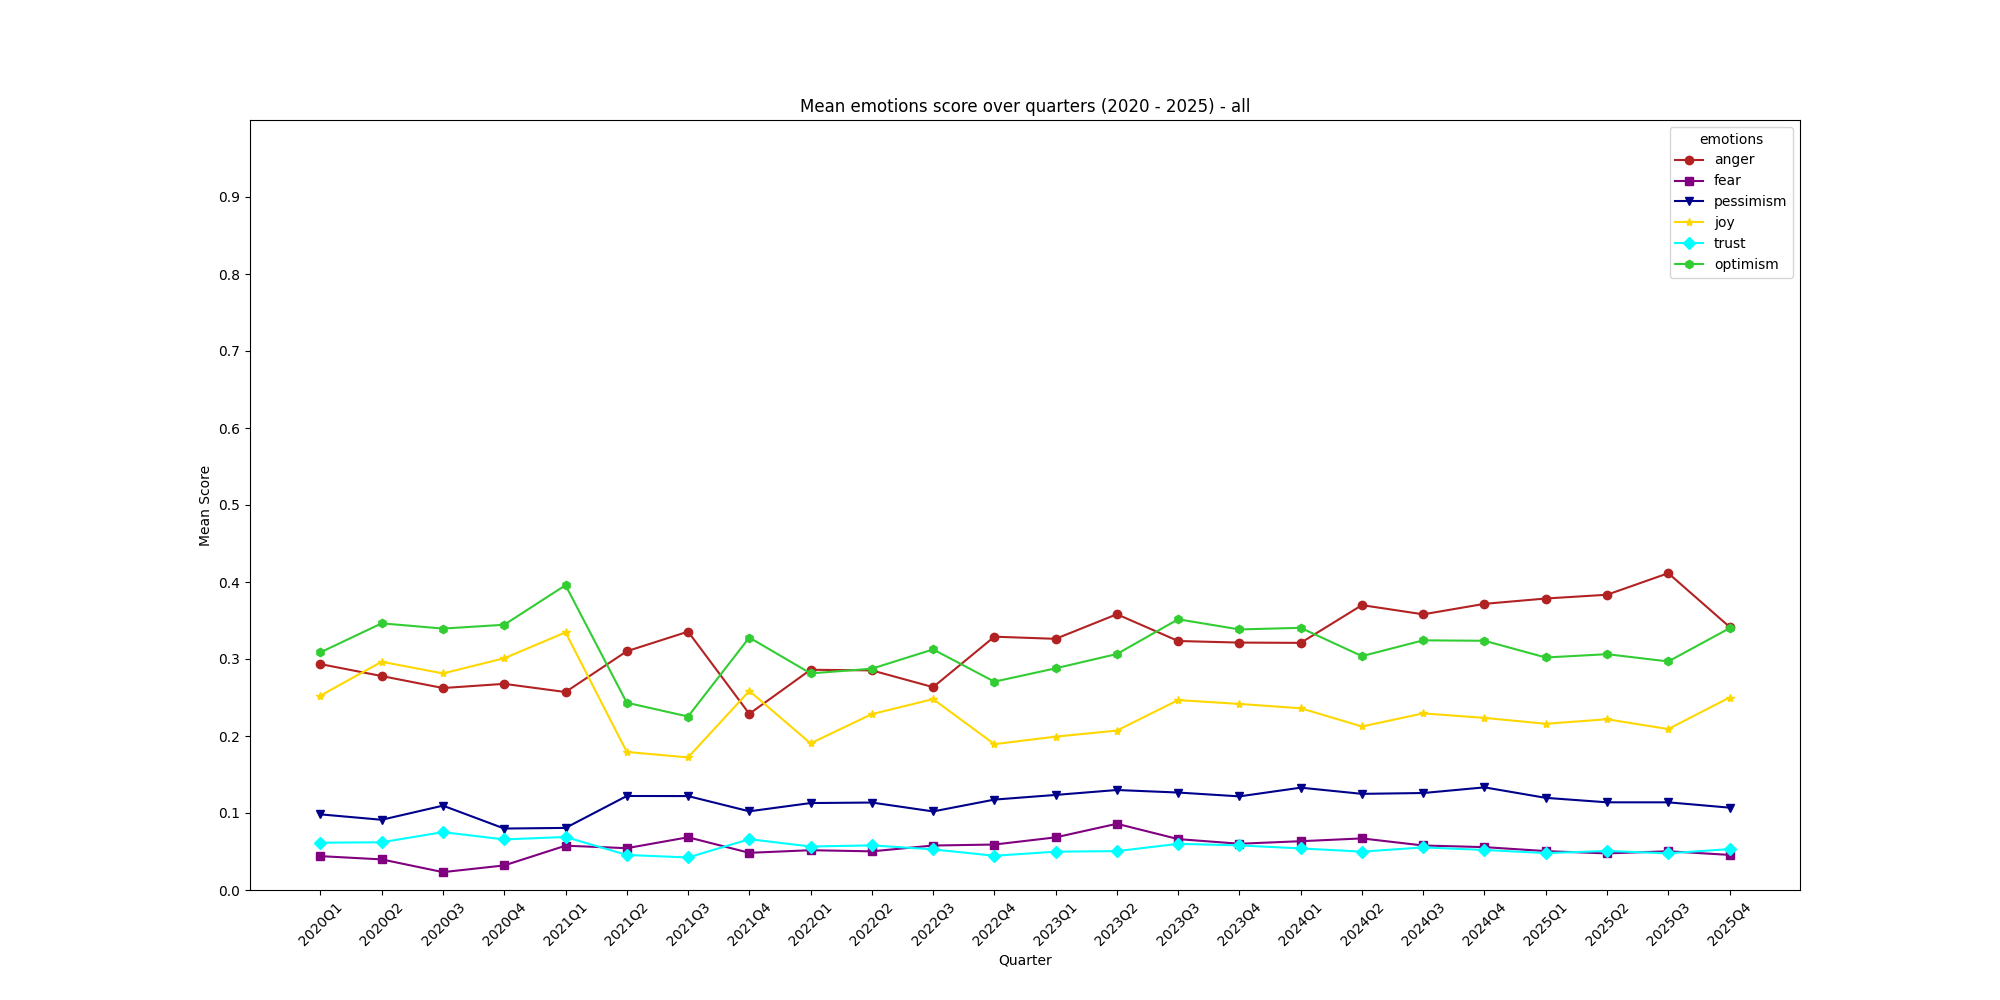
\includegraphics[width=0.95\linewidth]{Images/all_emotions.png}
    \caption{All comments emotions score}
\end{figure}
\begin{figure}[H]
    \centering
    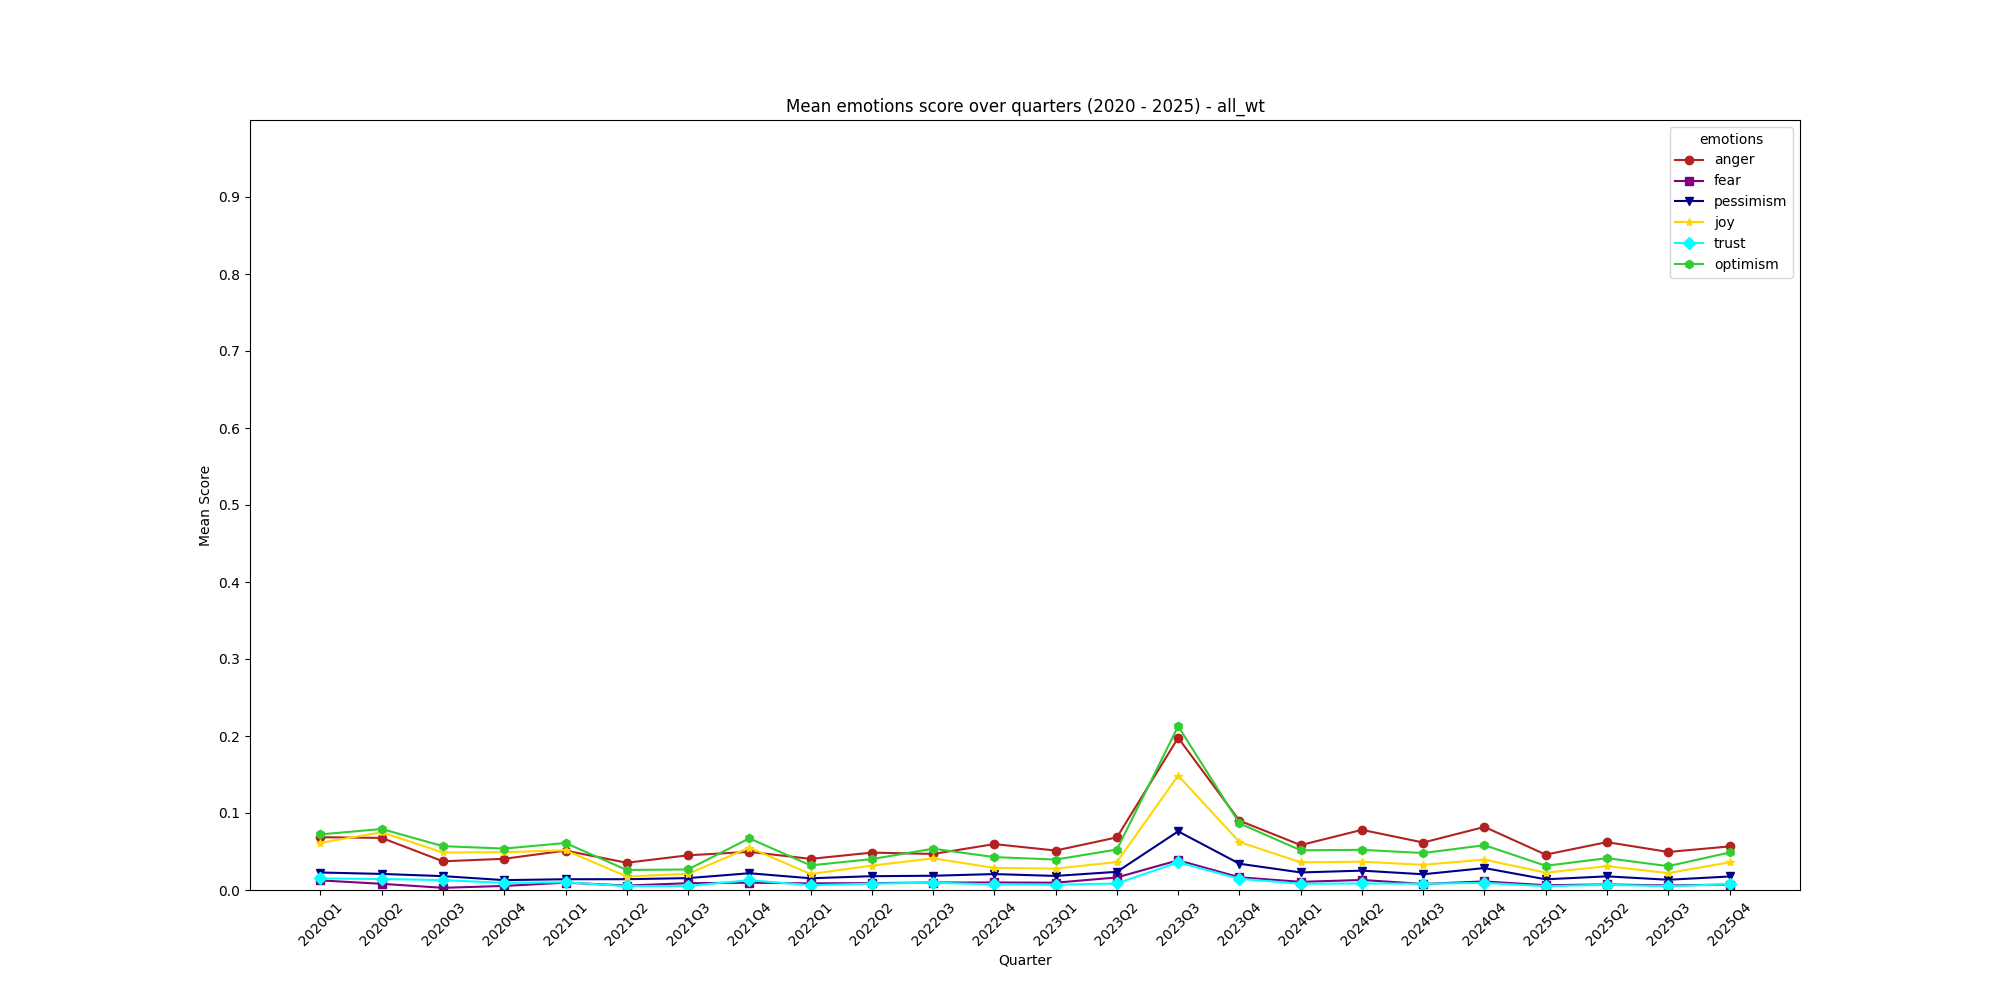
\includegraphics[width=0.95\linewidth]{Images/all_wt_emotions.png}
    \caption{All comments weighted emotions score}
\end{figure}

\subsection{BERTopic}

\begin{figure}[H]
    \centering
    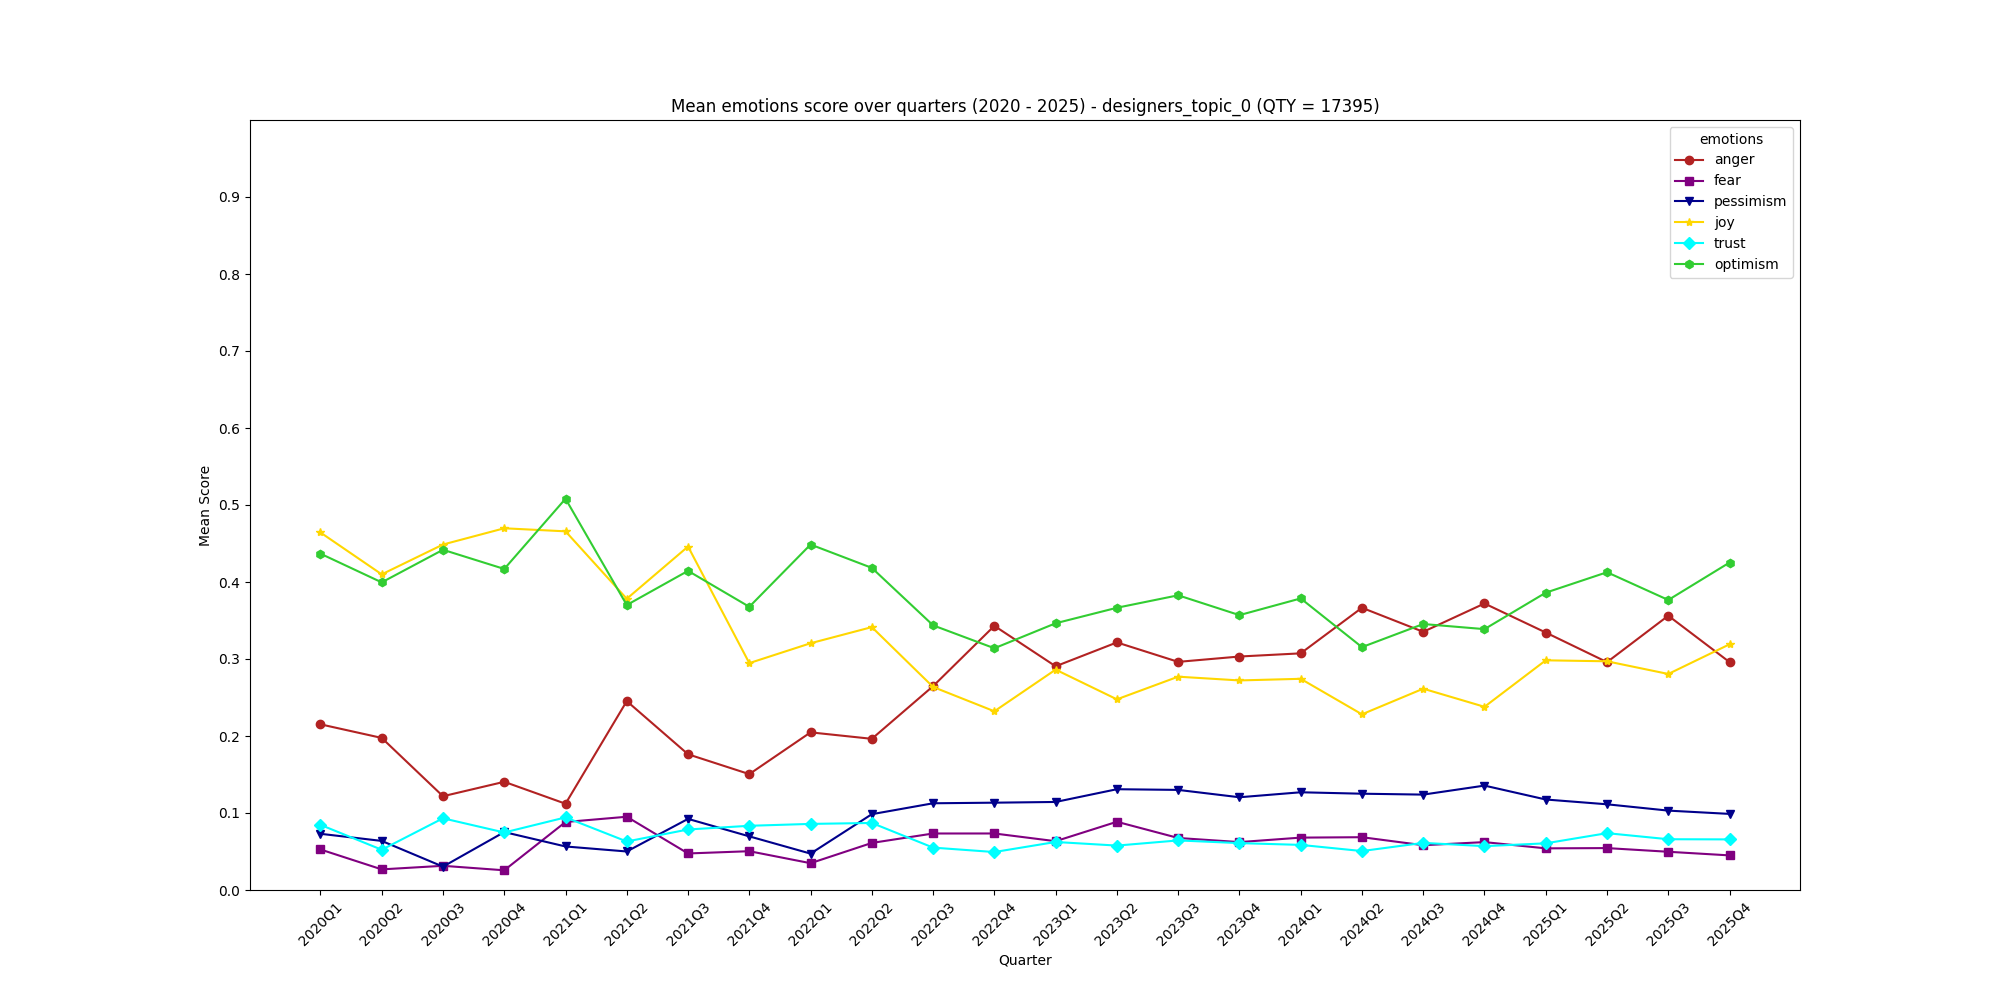
\includegraphics[width=0.80\linewidth]{Images/Appendices/Emotion/BERTopic/designers_topic_0_emotions.png}
    \caption{Designers topic 0}
\end{figure}
\begin{figure}[H]
    \centering
    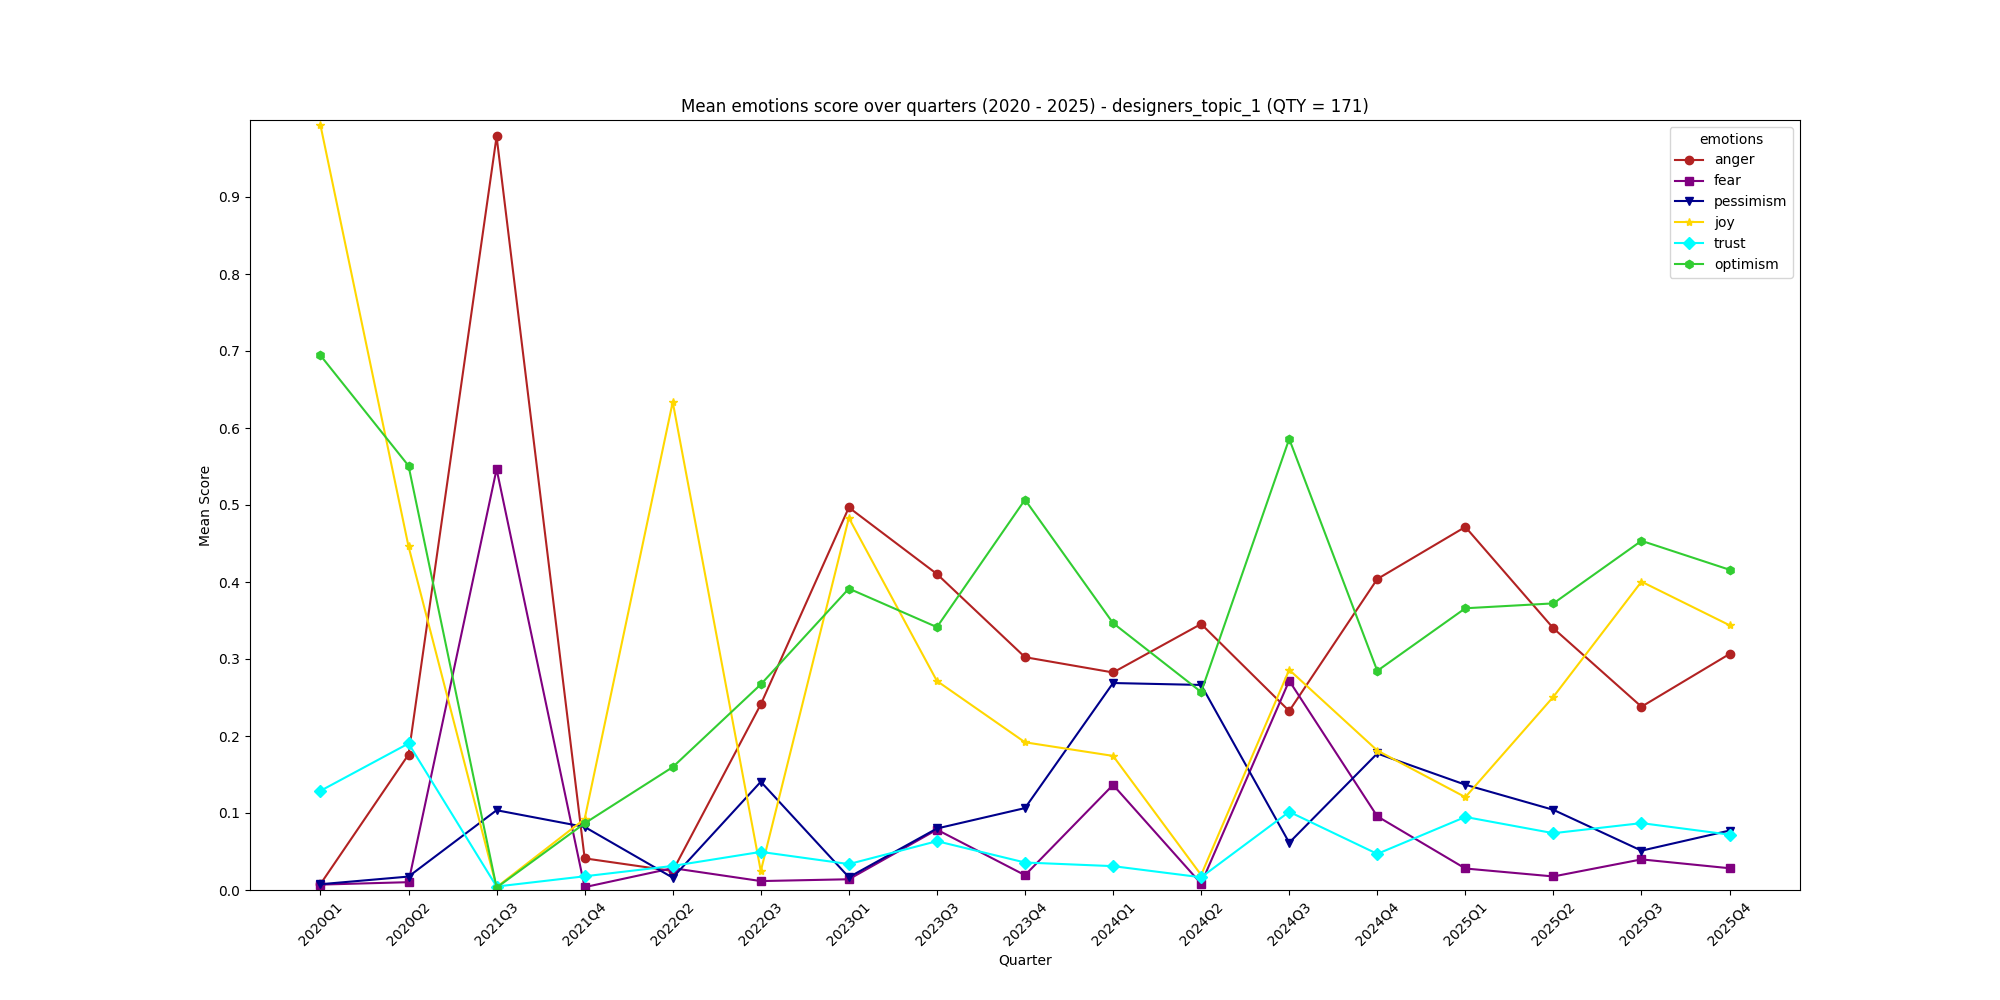
\includegraphics[width=0.80\linewidth]{Images/Appendices/Emotion/BERTopic/designers_topic_1_emotions.png}
    \caption{Designers topic 1}
\end{figure}
\begin{figure}[H]
    \centering
    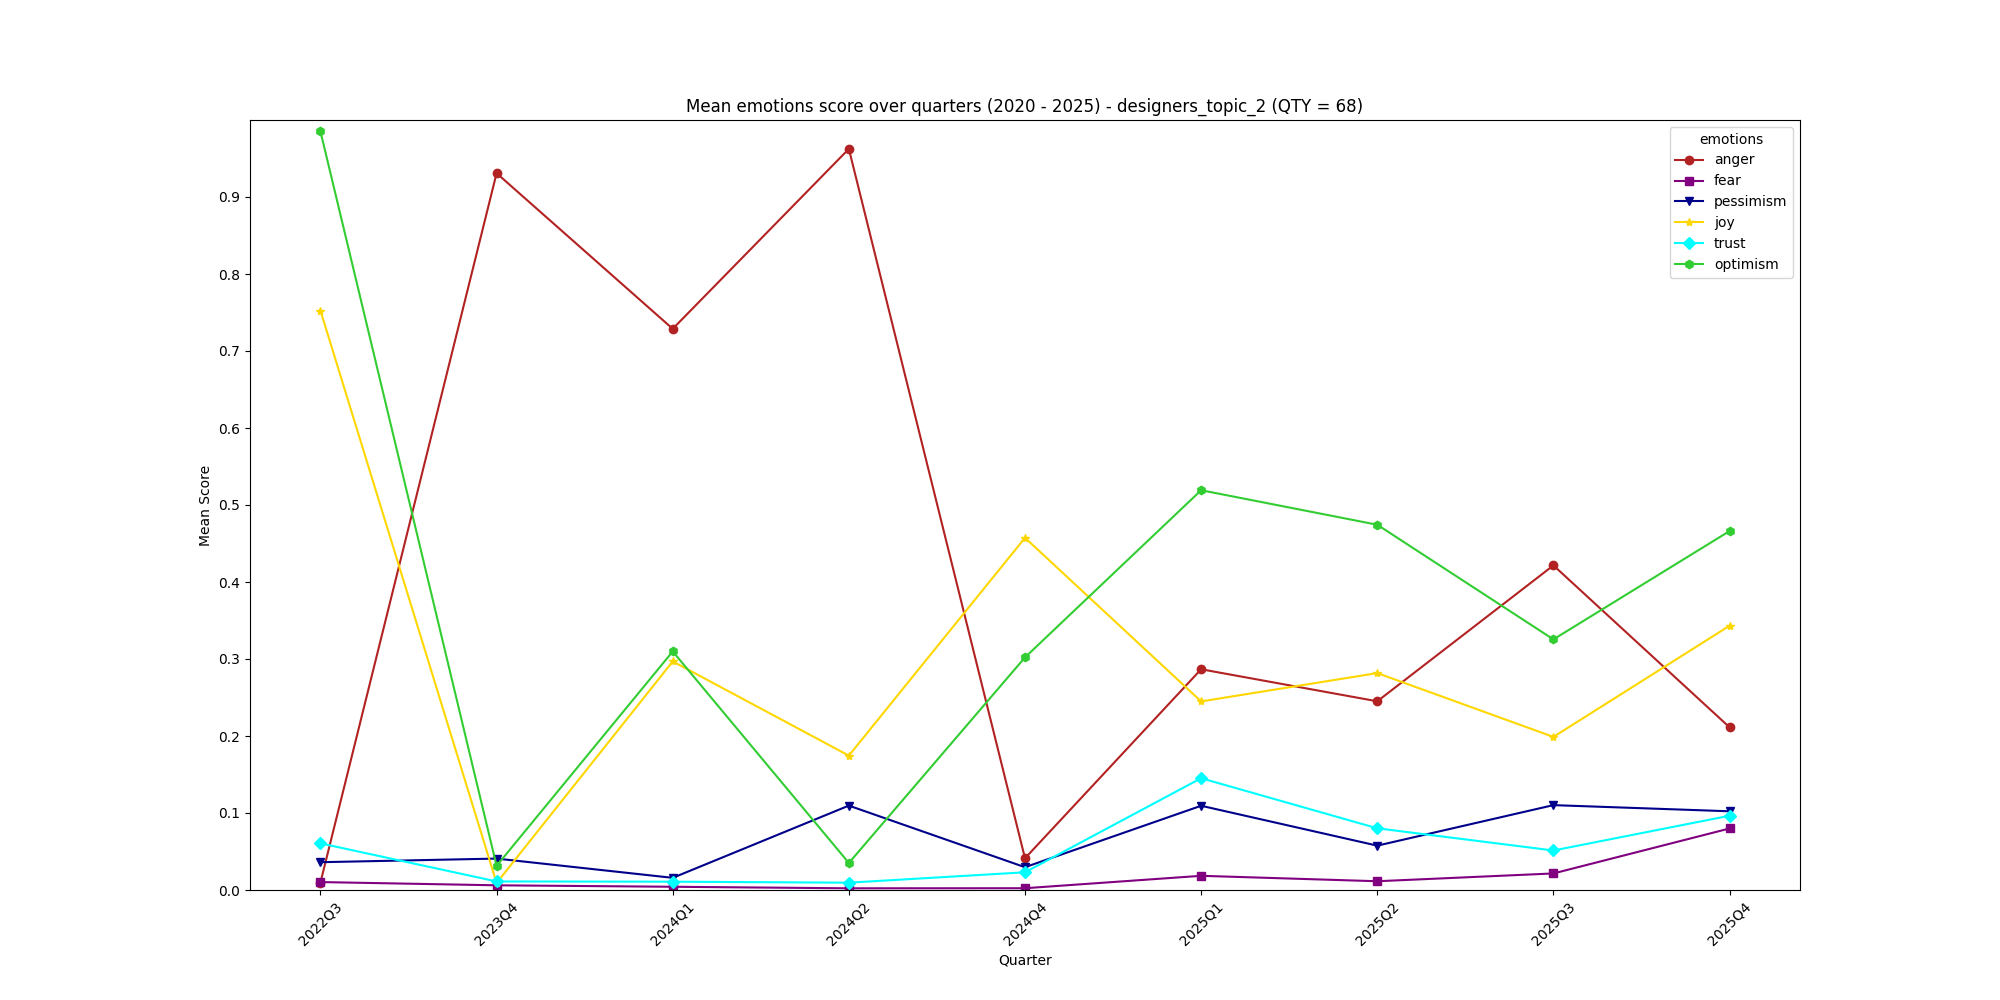
\includegraphics[width=0.80\linewidth]{Images/Appendices/Emotion/BERTopic/designers_topic_2_emotions.png}
    \caption{Designers topic 2}
\end{figure}
\begin{figure}[H]
    \centering
    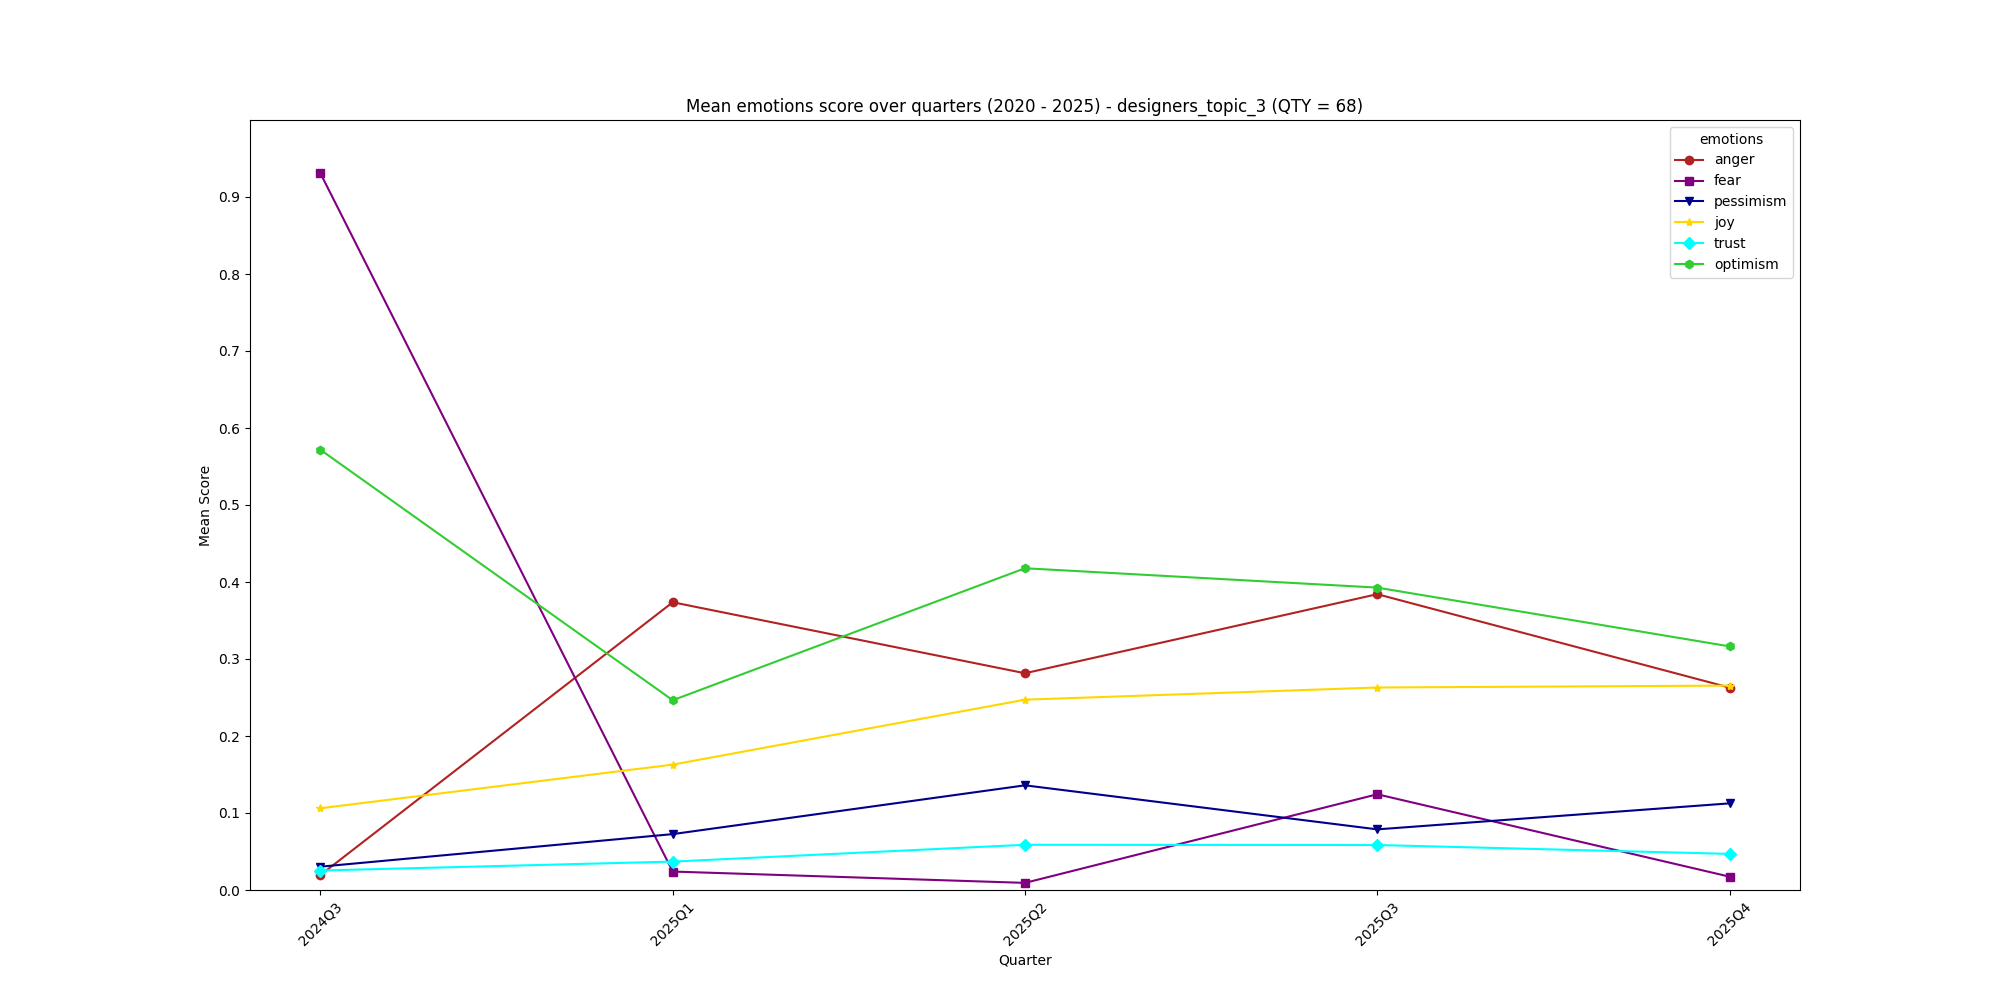
\includegraphics[width=0.80\linewidth]{Images/Appendices/Emotion/BERTopic/designers_topic_3_emotions.png}
    \caption{Designers topic 3}
\end{figure}
\begin{figure}[H]
    \centering
    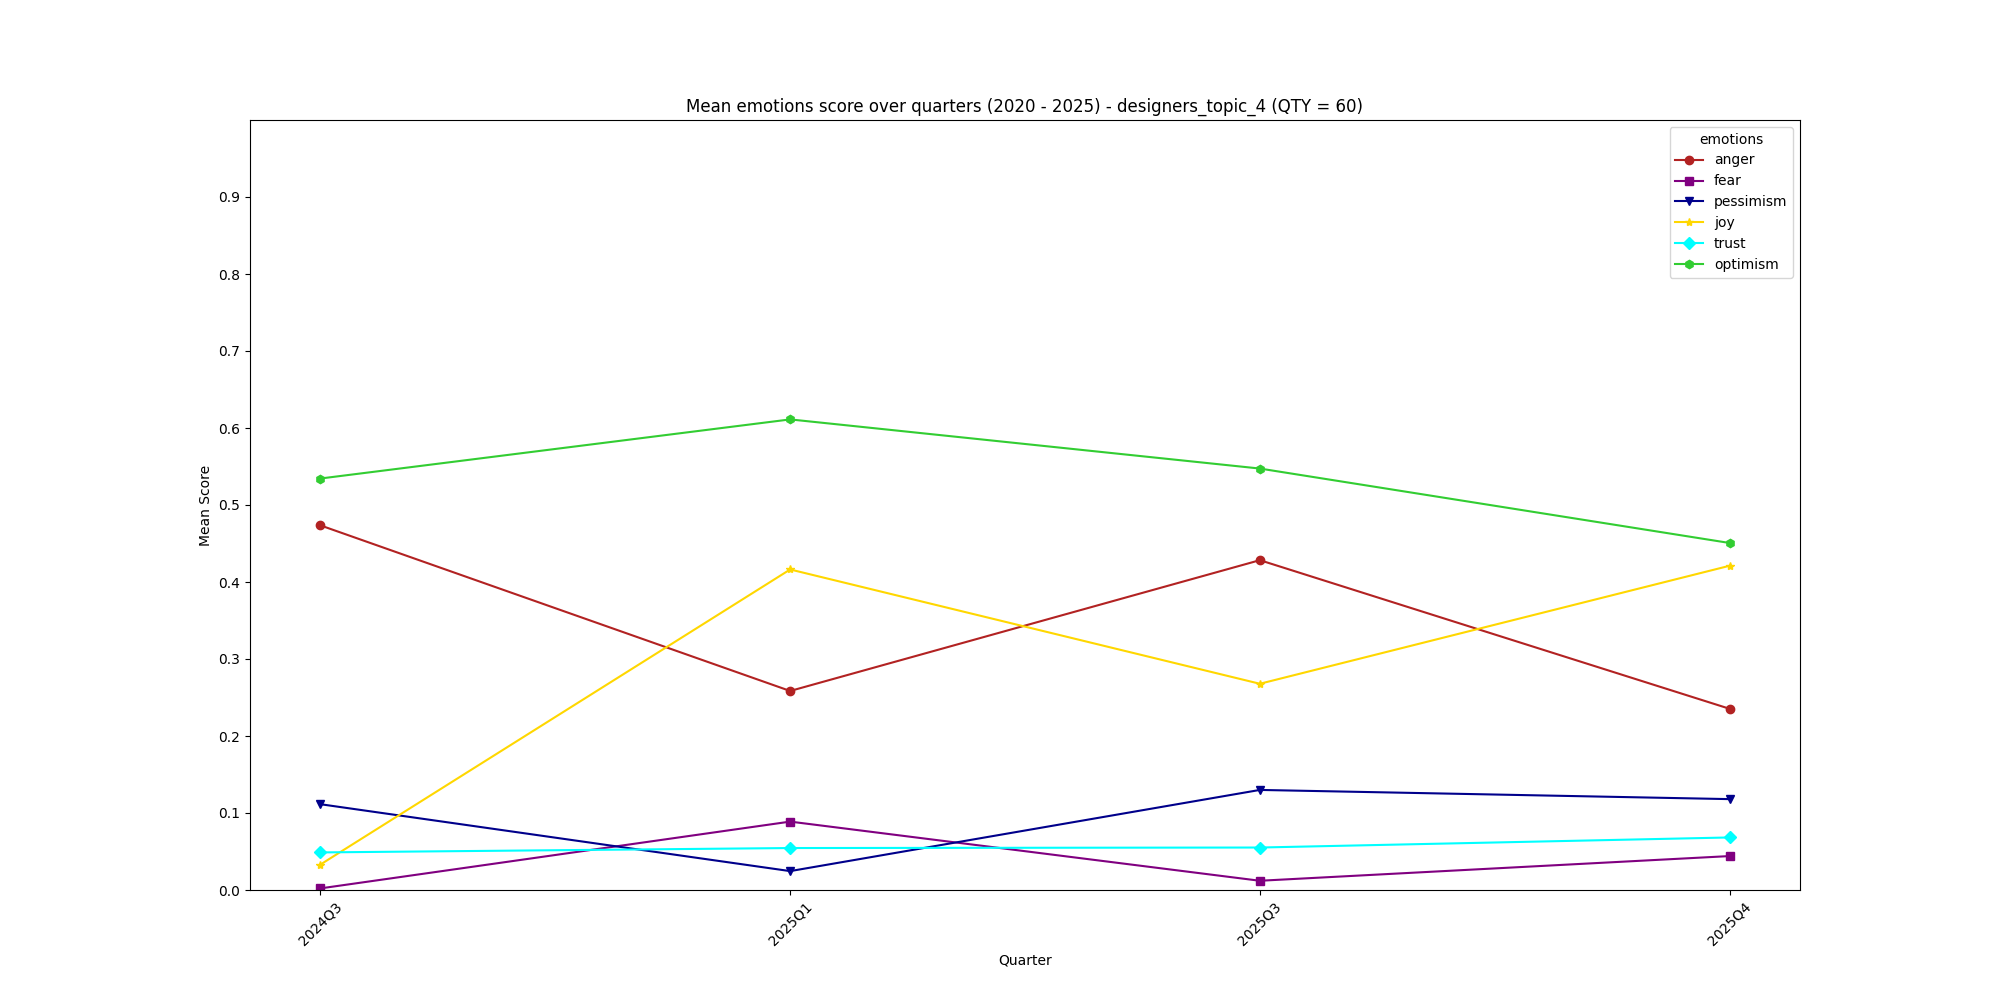
\includegraphics[width=0.80\linewidth]{Images/Appendices/Emotion/BERTopic/designers_topic_4_emotions.png}
    \caption{Designers topic 4}
\end{figure}
\begin{figure}[H]
    \centering
    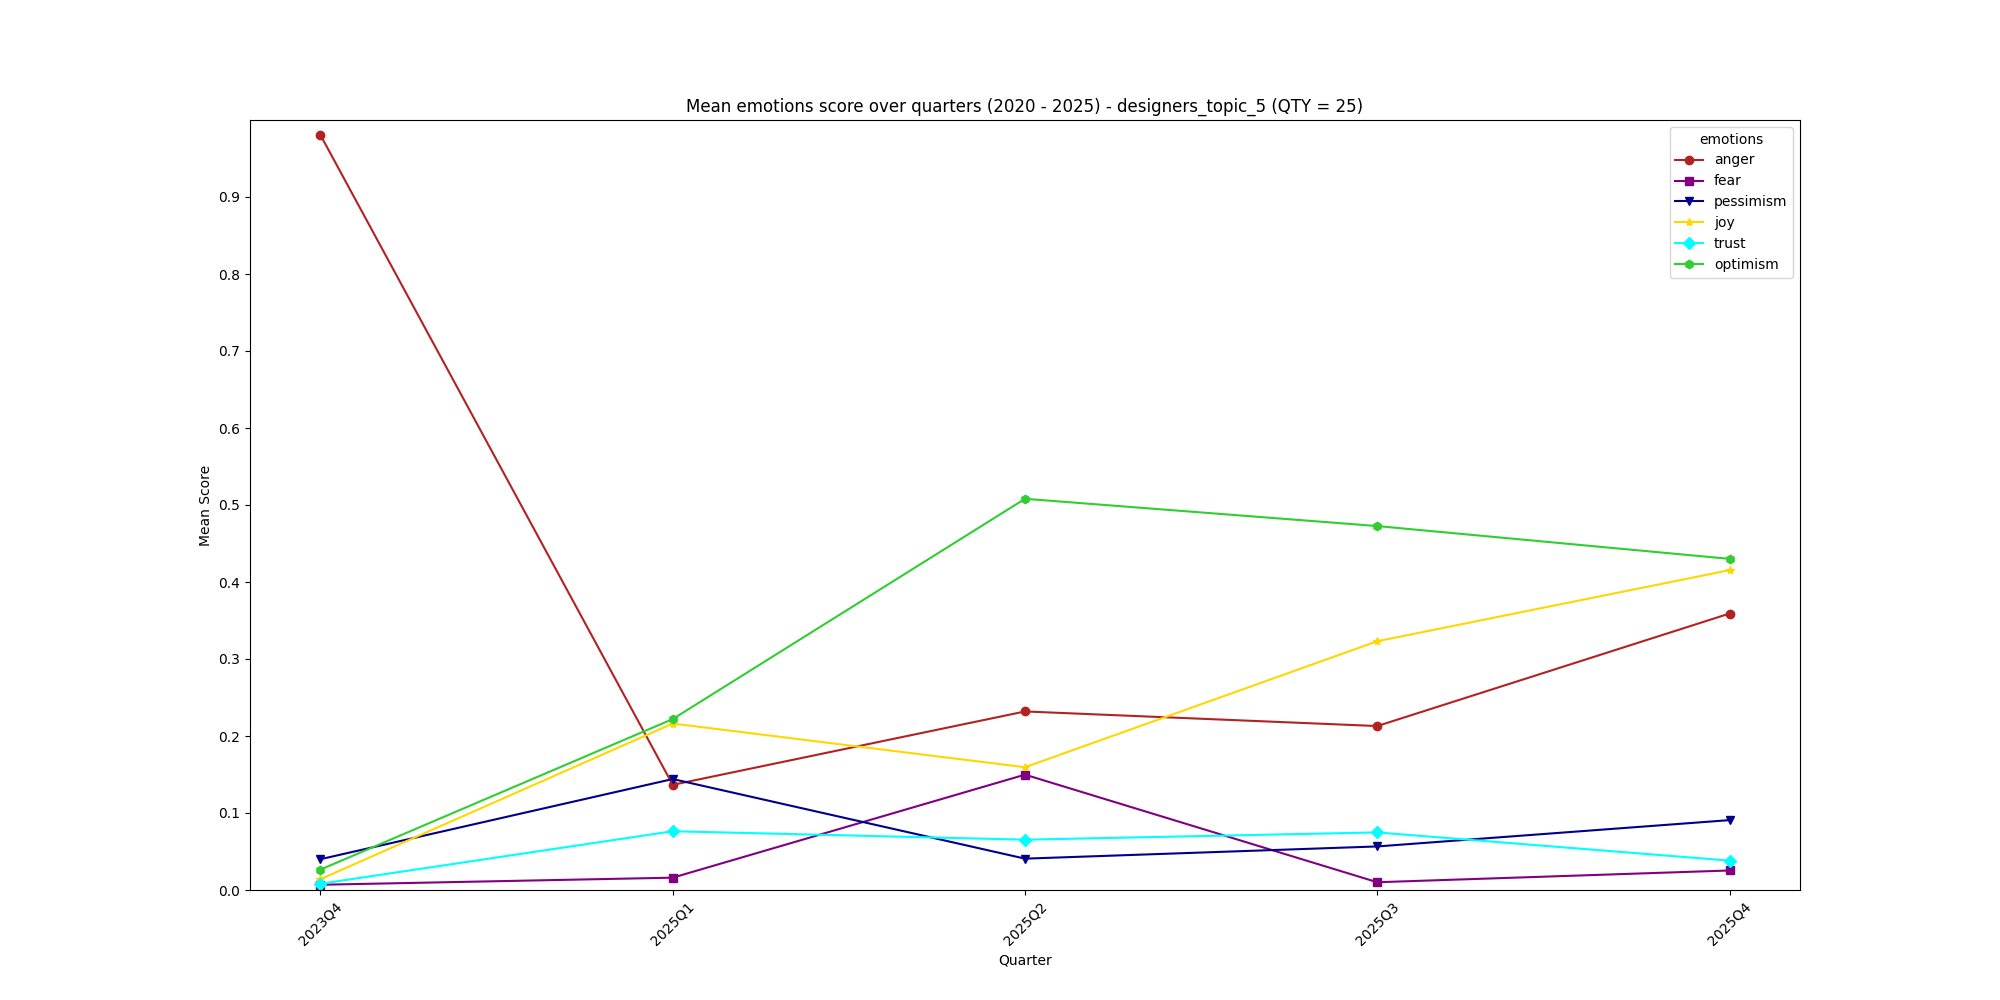
\includegraphics[width=0.80\linewidth]{Images/Appendices/Emotion/BERTopic/designers_topic_5_emotions.png}
    \caption{Designers topic 5}
\end{figure}
\begin{figure}[H]
    \centering
    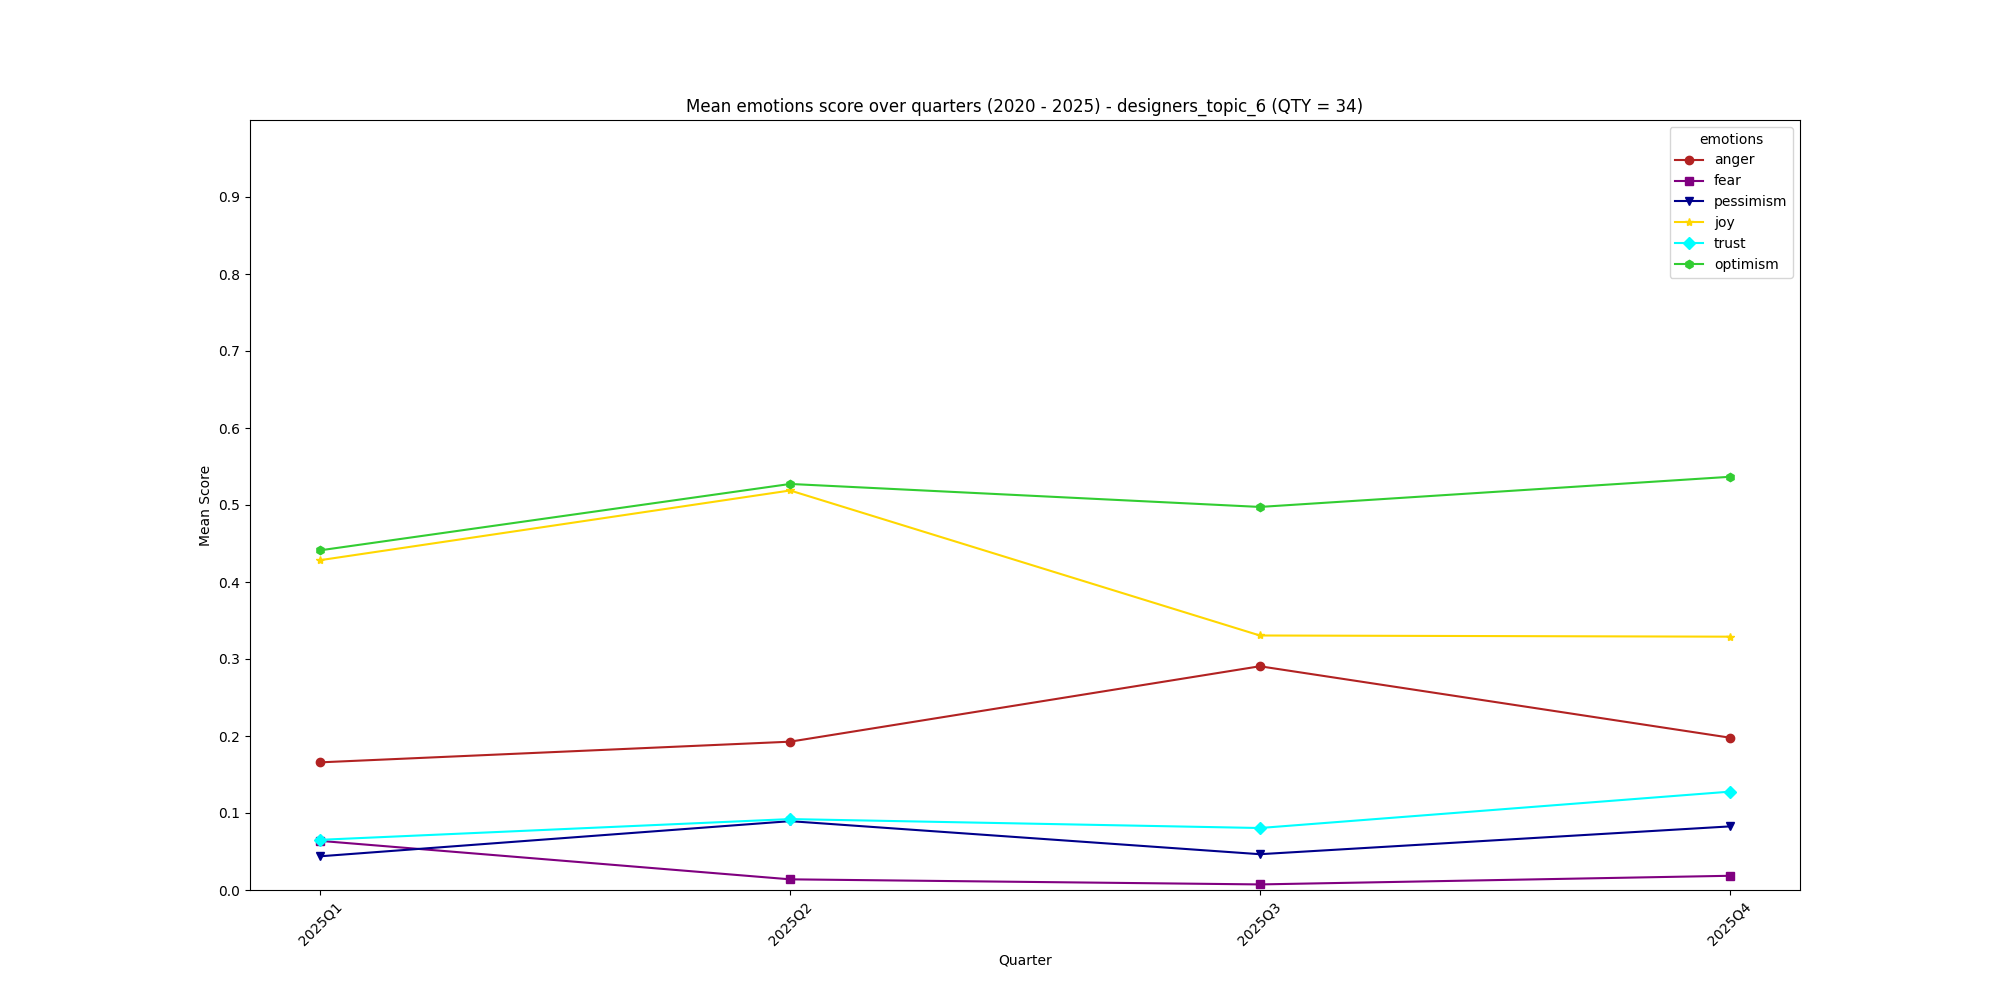
\includegraphics[width=0.80\linewidth]{Images/Appendices/Emotion/BERTopic/designers_topic_6_emotions.png}
    \caption{Designers topic 6}
\end{figure}

\begin{figure}[H]
    \centering
    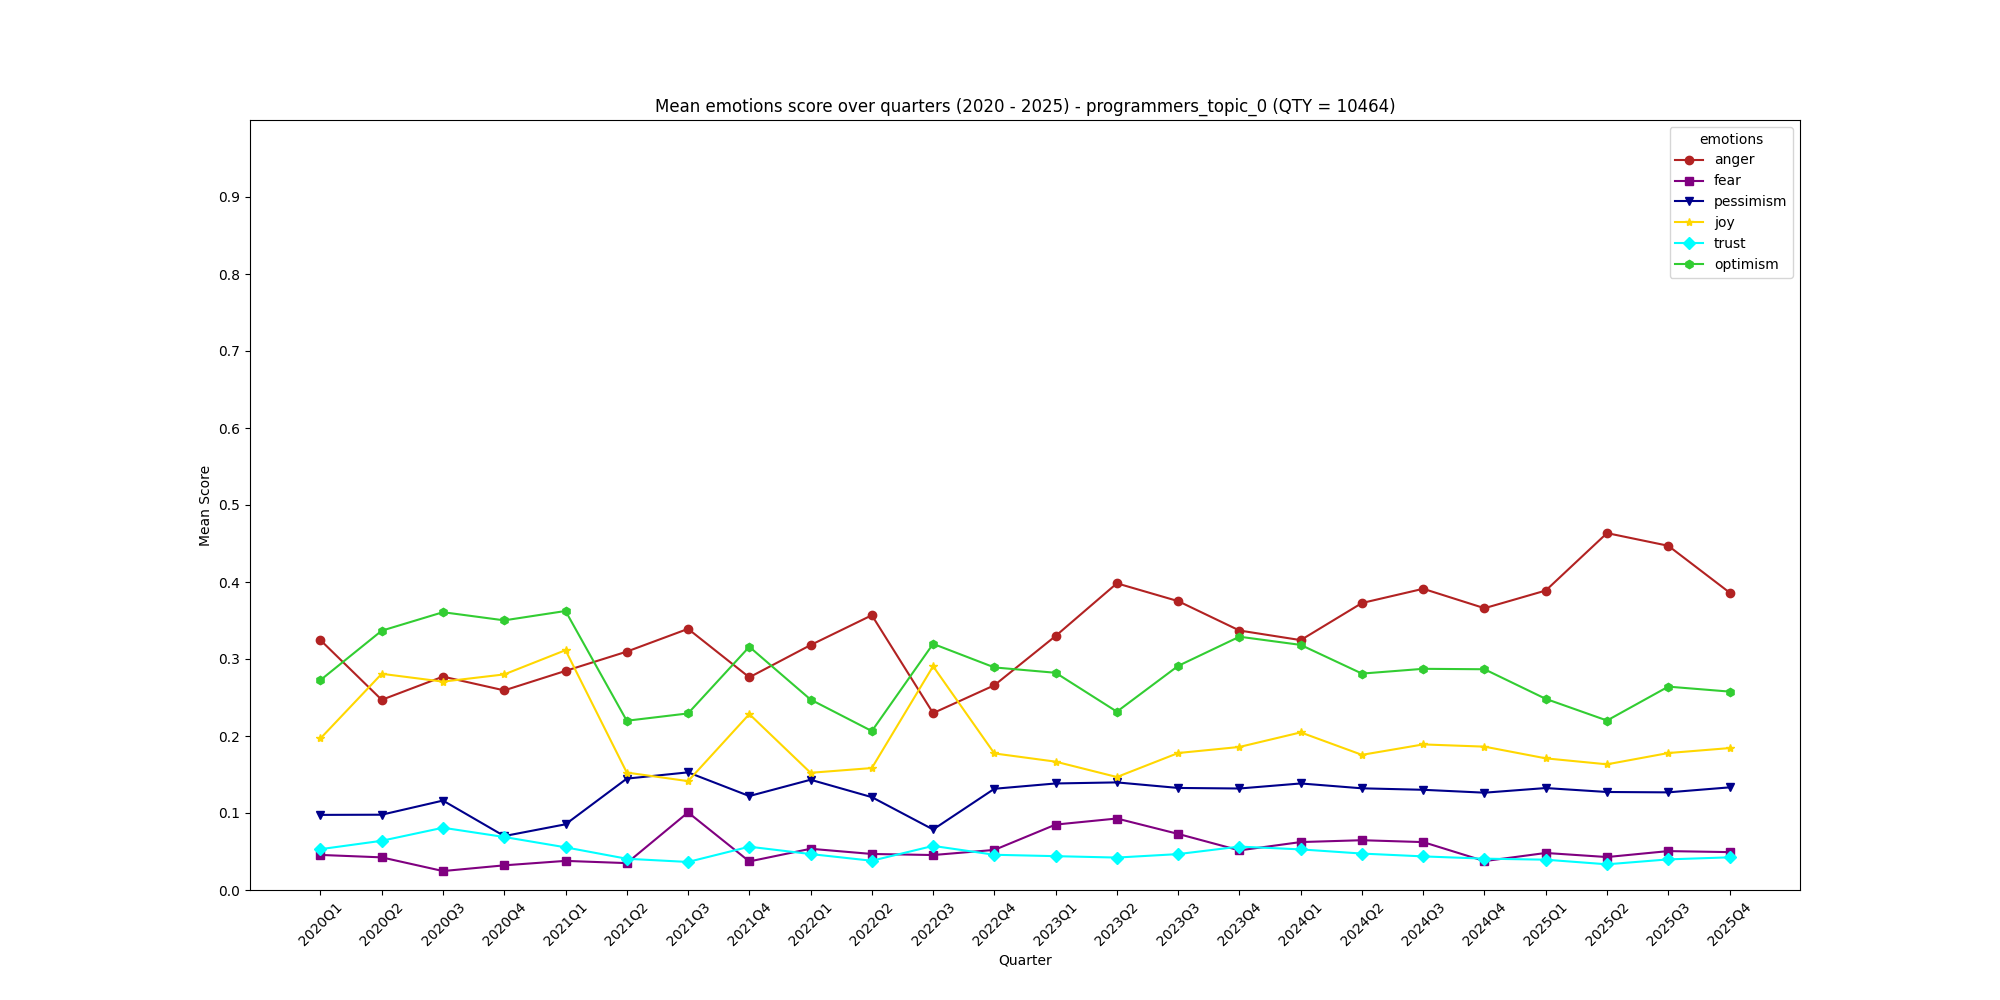
\includegraphics[width=0.80\linewidth]{Images/Appendices/Emotion/BERTopic/programmers_topic_0_emotions.png}
    \caption{Programmers topic 0}
\end{figure}
\begin{figure}[H]
    \centering
    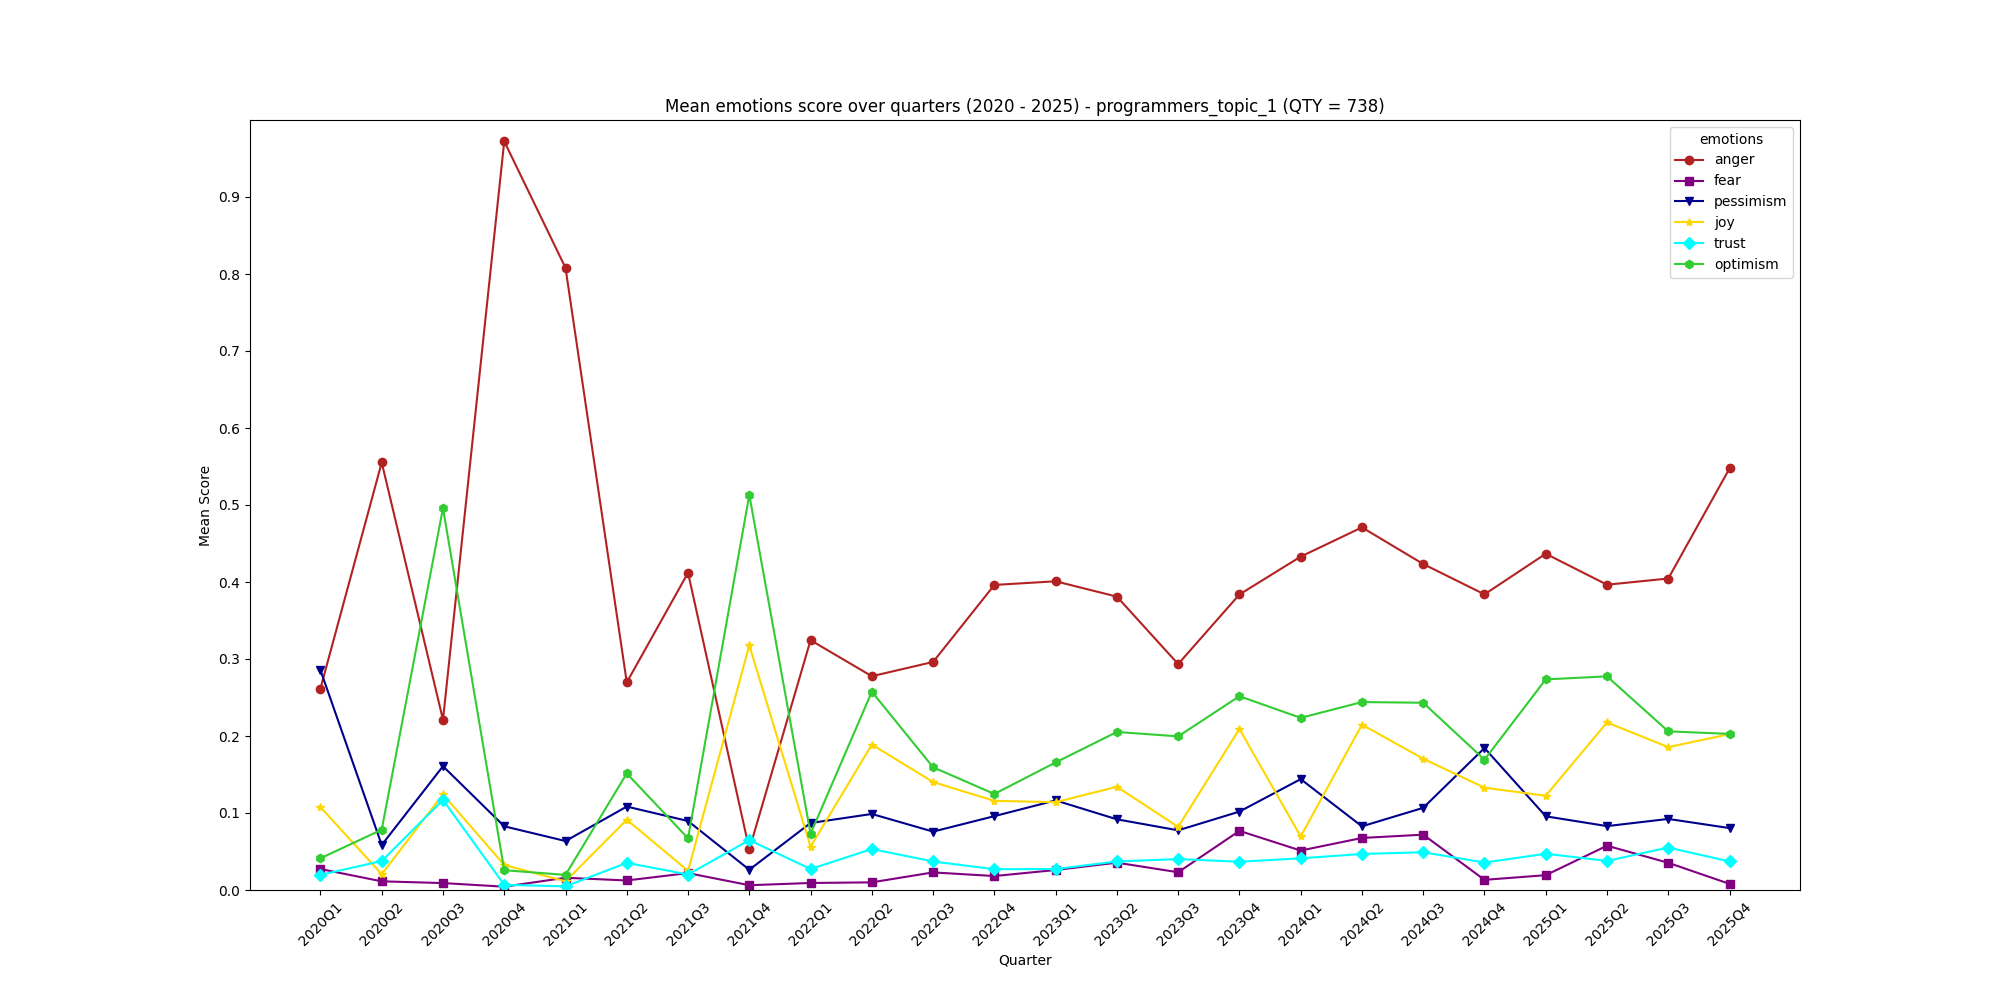
\includegraphics[width=0.80\linewidth]{Images/Appendices/Emotion/BERTopic/programmers_topic_1_emotions.png}
    \caption{Programmers topic 1}
\end{figure}
\begin{figure}[H]
    \centering
    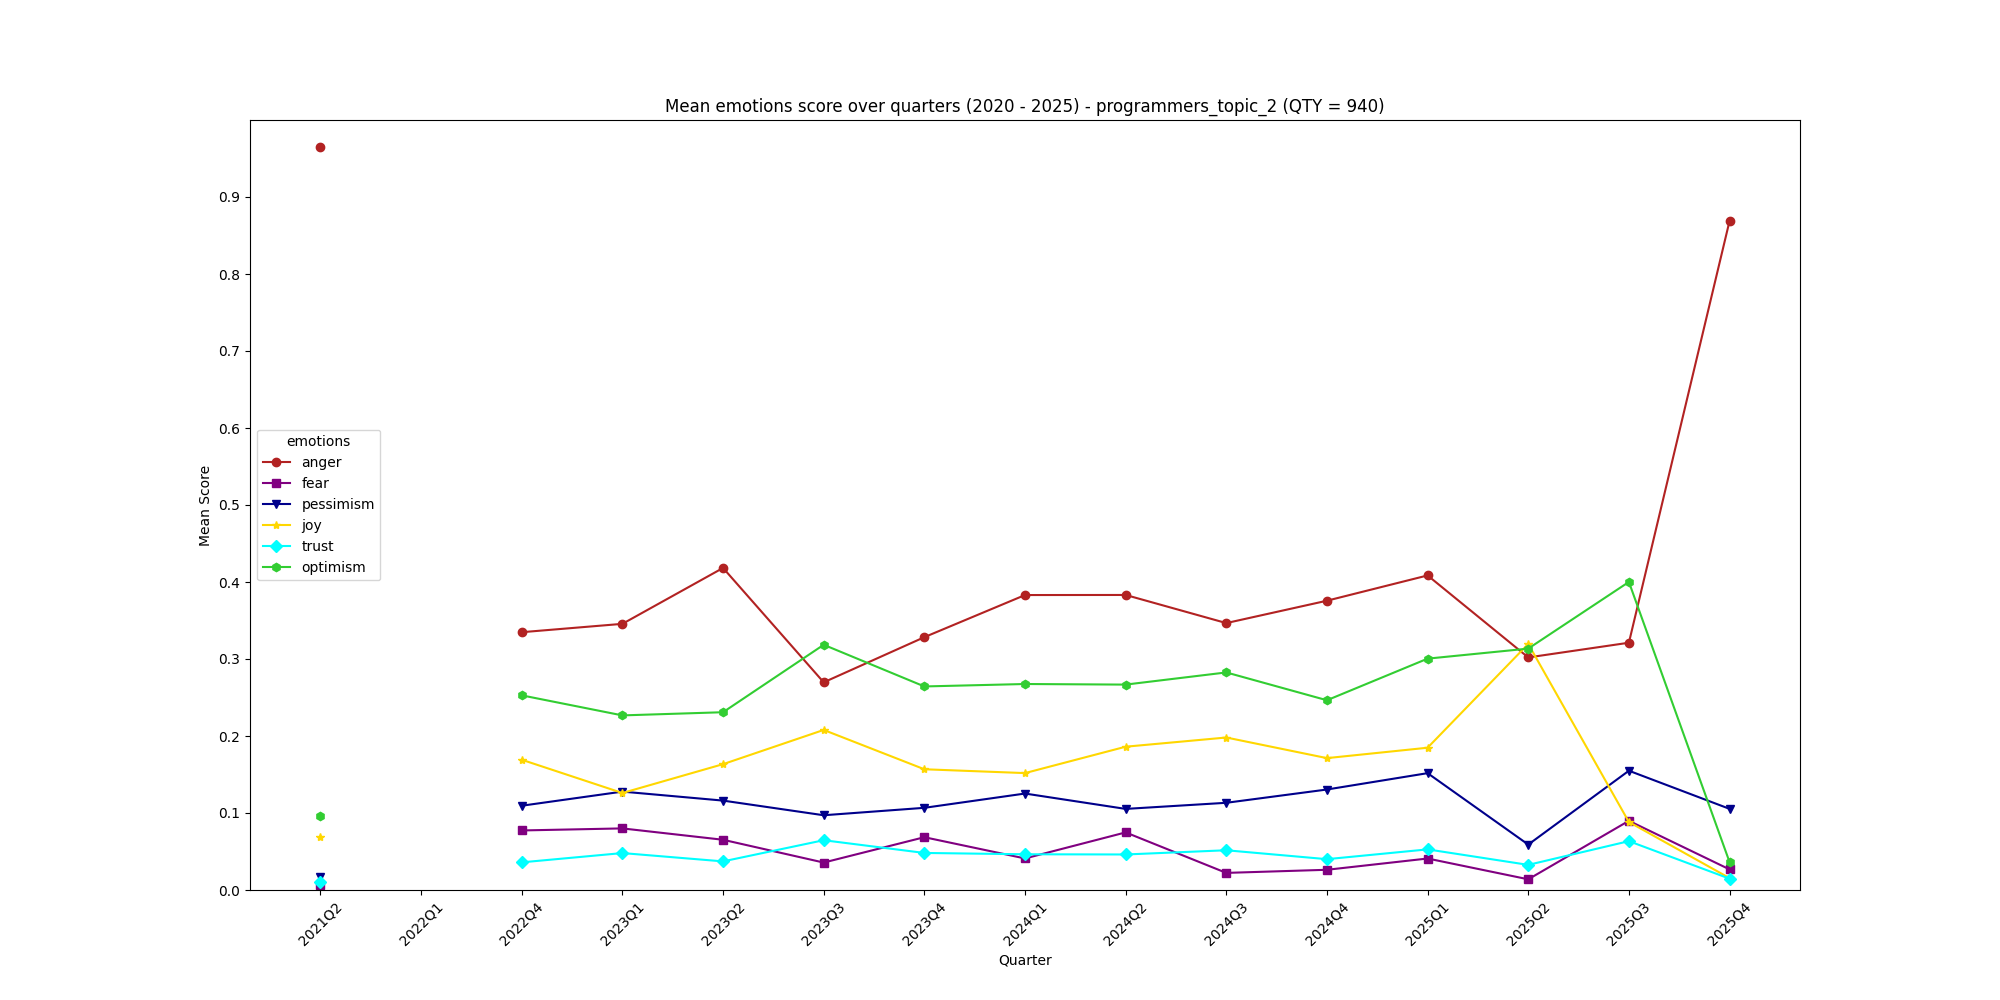
\includegraphics[width=0.80\linewidth]{Images/Appendices/Emotion/BERTopic/programmers_topic_2_emotions.png}
    \caption{Programmers topic 2}
\end{figure}
\begin{figure}[H]
    \centering
    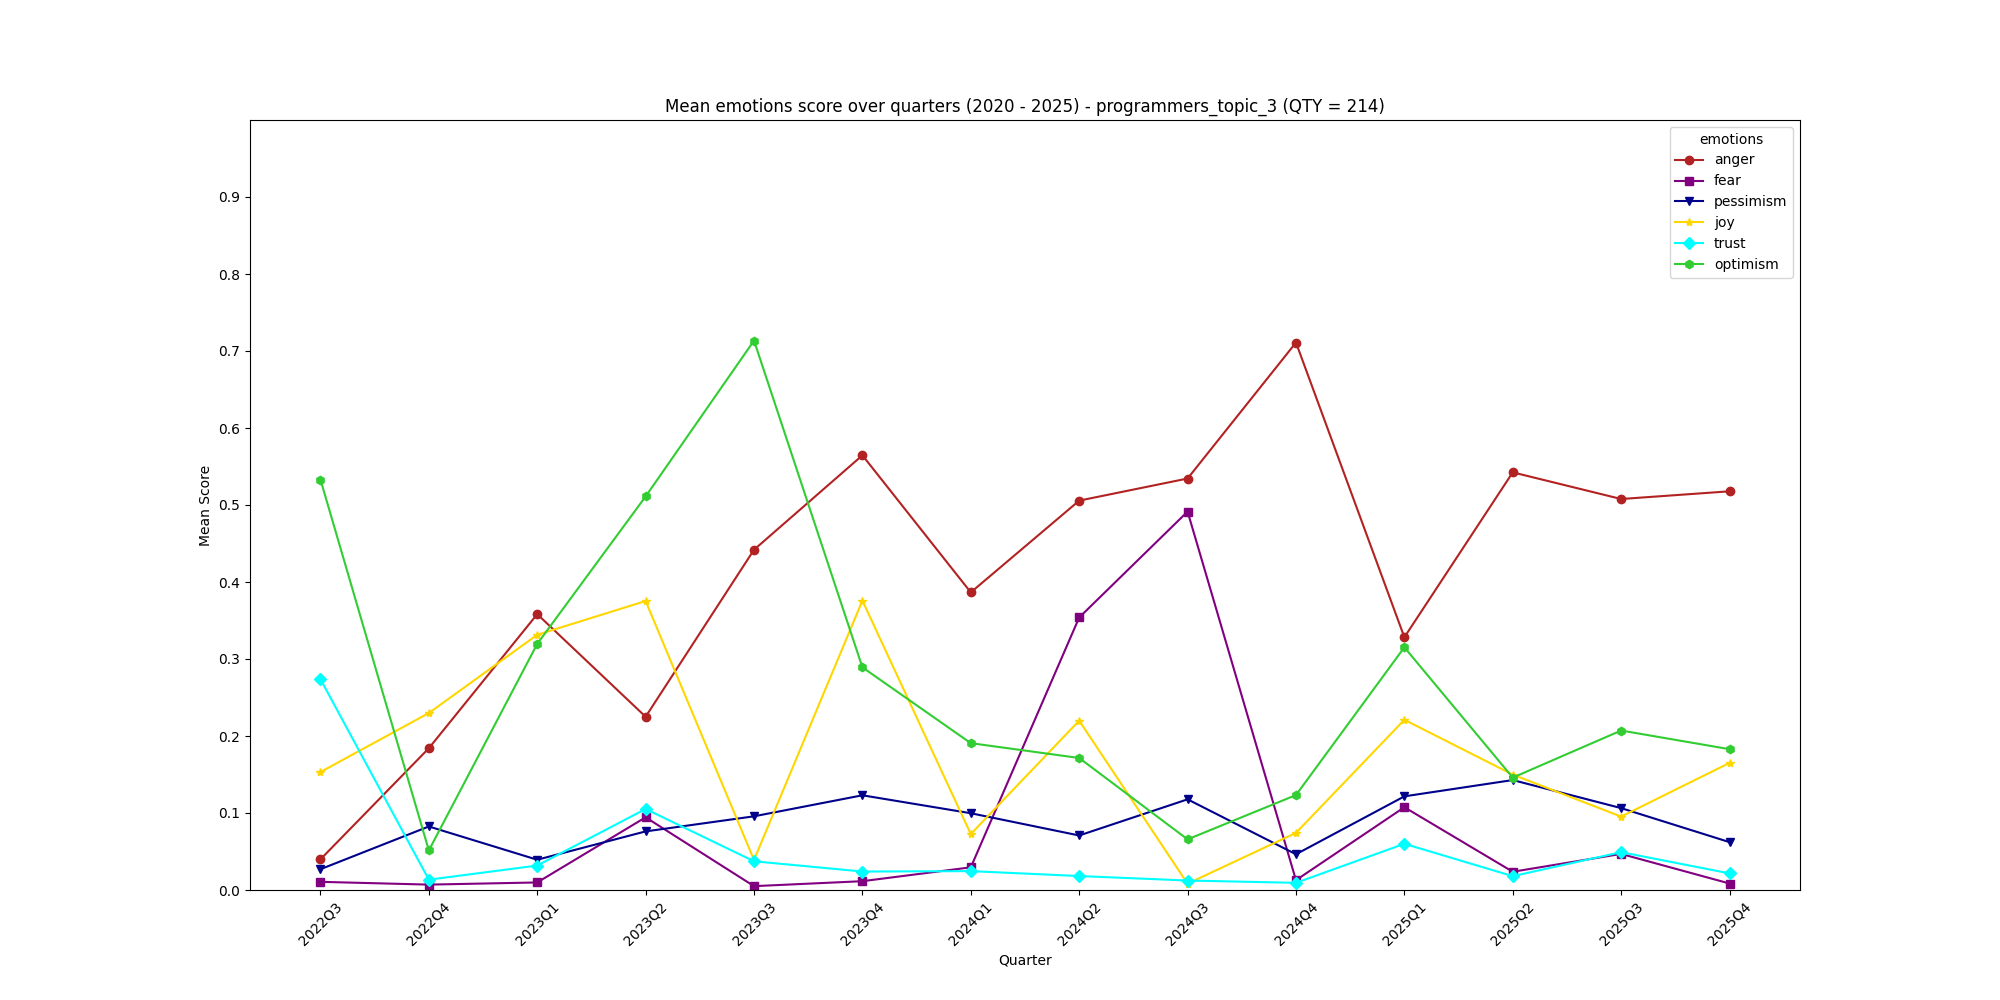
\includegraphics[width=0.80\linewidth]{Images/Appendices/Emotion/BERTopic/programmers_topic_3_emotions.png}
    \caption{Programmers topic 3}
\end{figure}
\begin{figure}[H]
    \centering
    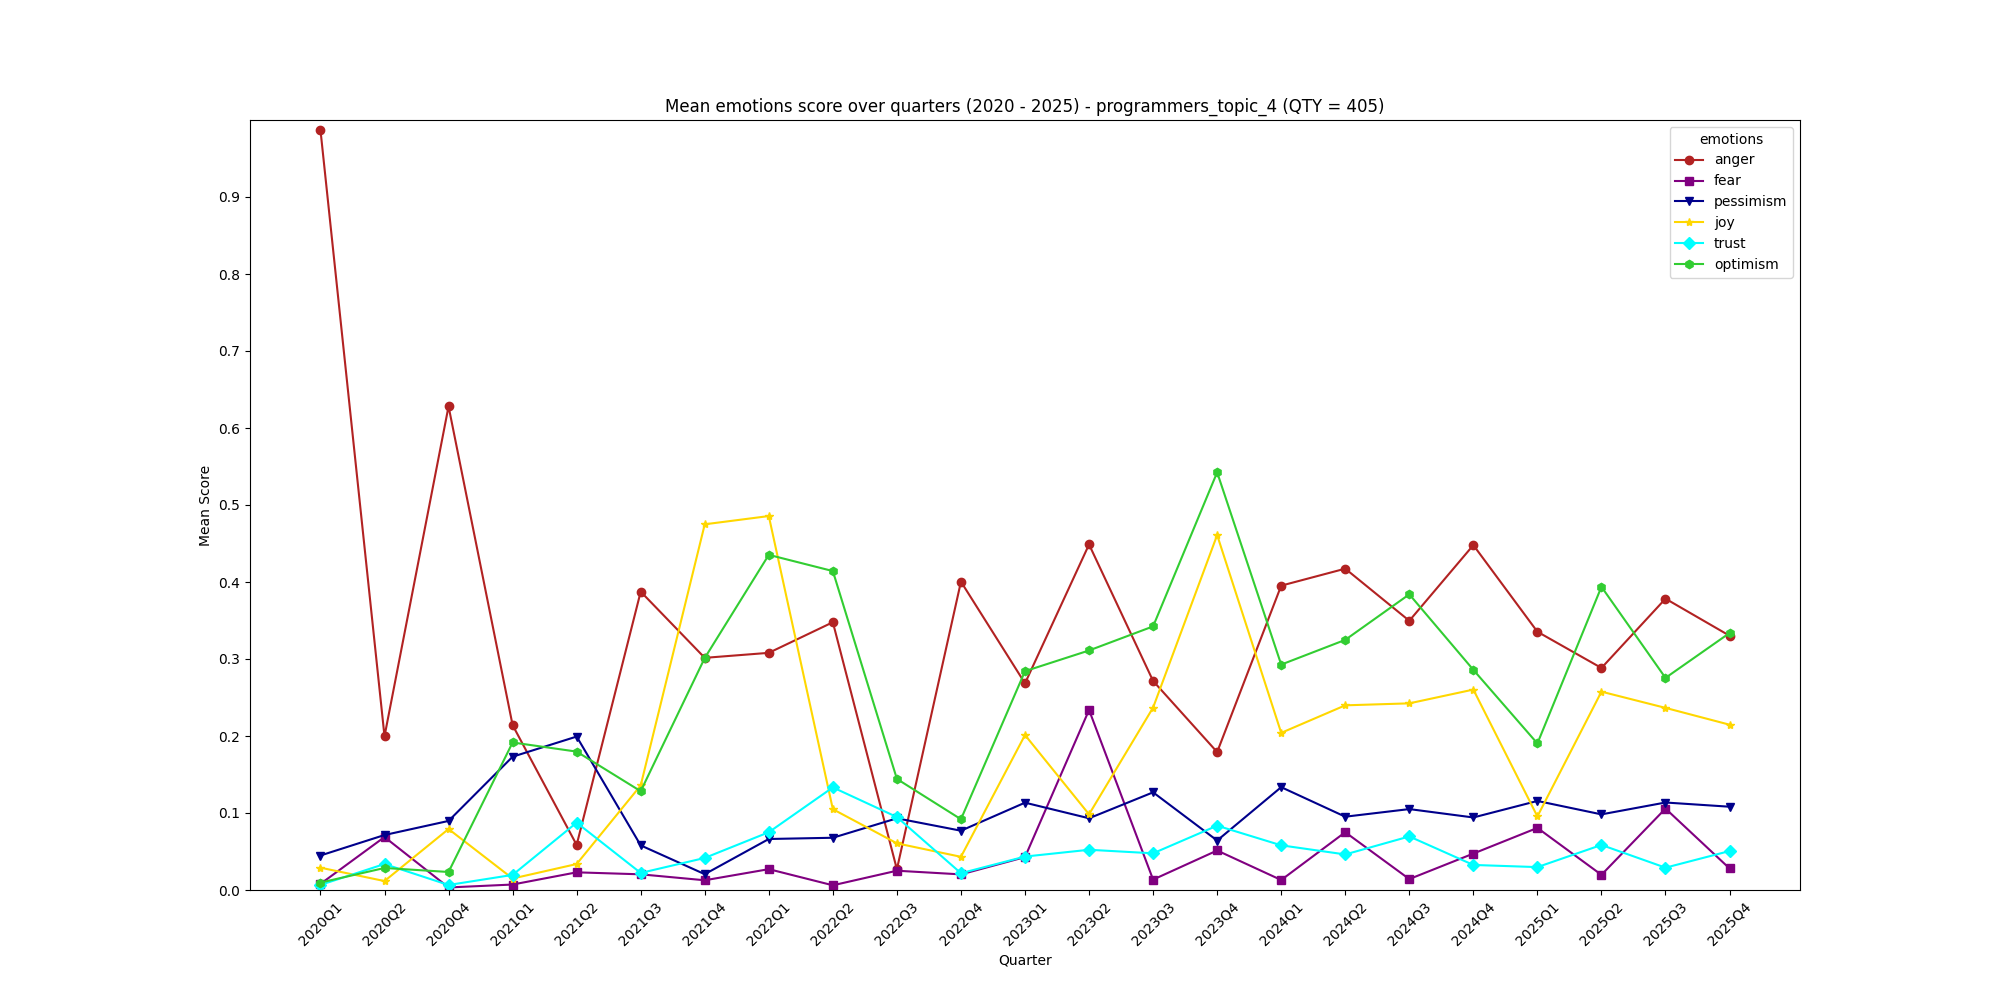
\includegraphics[width=0.80\linewidth]{Images/Appendices/Emotion/BERTopic/programmers_topic_4_emotions.png}
    \caption{Programmers topic 4}
\end{figure}
\begin{figure}[H]
    \centering
    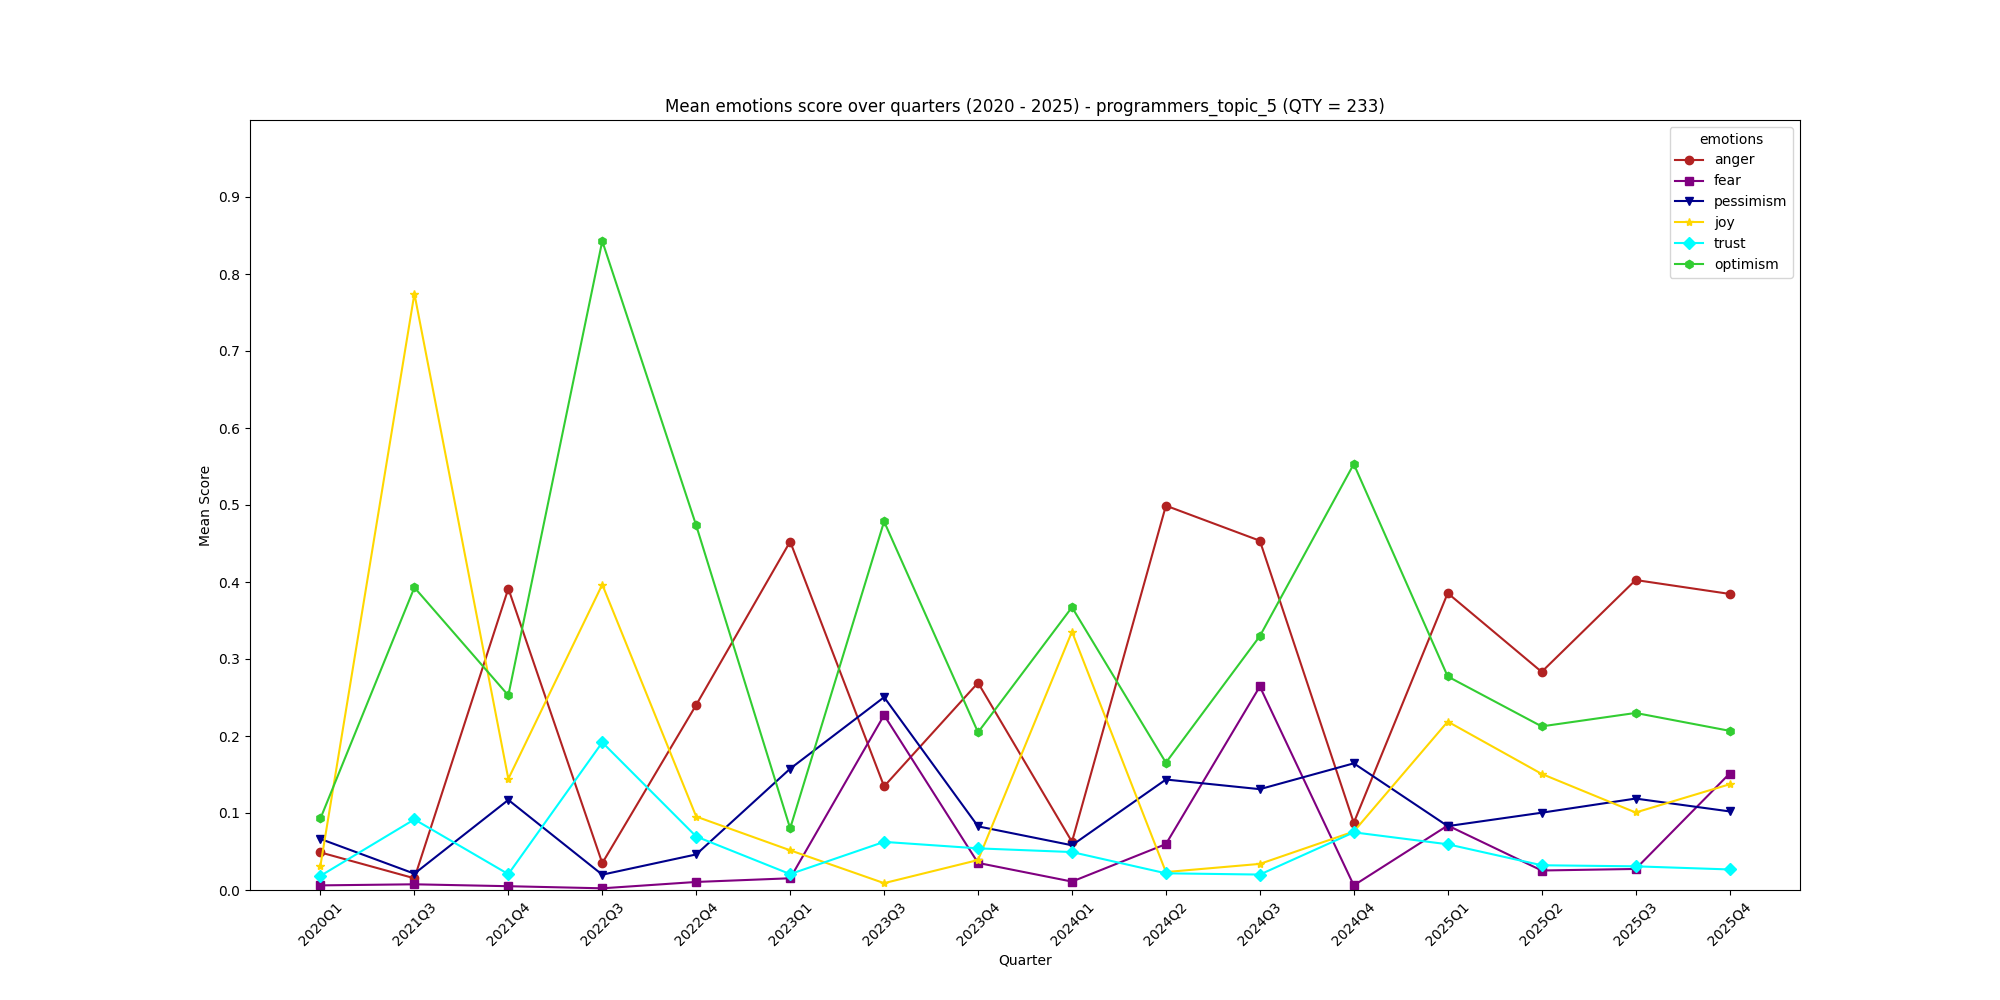
\includegraphics[width=0.80\linewidth]{Images/Appendices/Emotion/BERTopic/programmers_topic_5_emotions.png}
    \caption{Programmers topic 5}
\end{figure}
\begin{figure}[H]
    \centering
    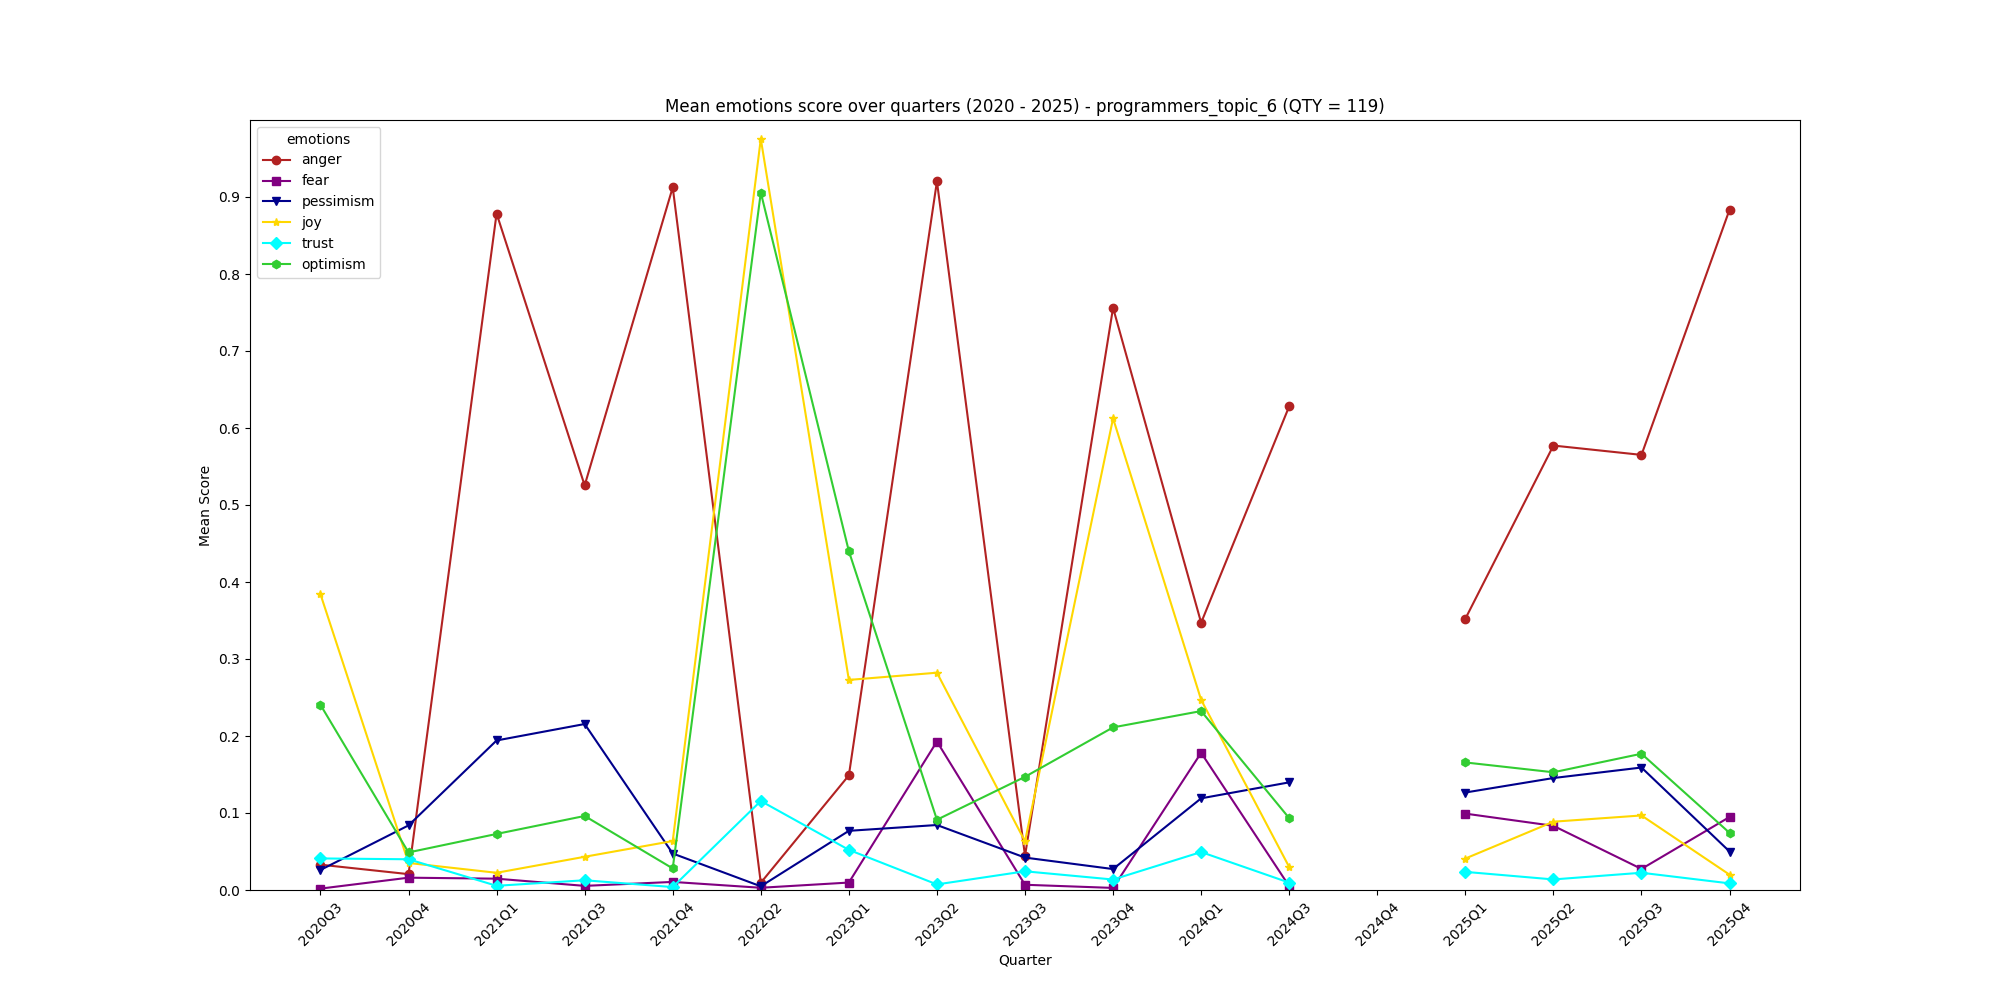
\includegraphics[width=0.80\linewidth]{Images/Appendices/Emotion/BERTopic/programmers_topic_6_emotions.png}
    \caption{Programmers topic 6}
\end{figure}
\begin{figure}[H]
    \centering
    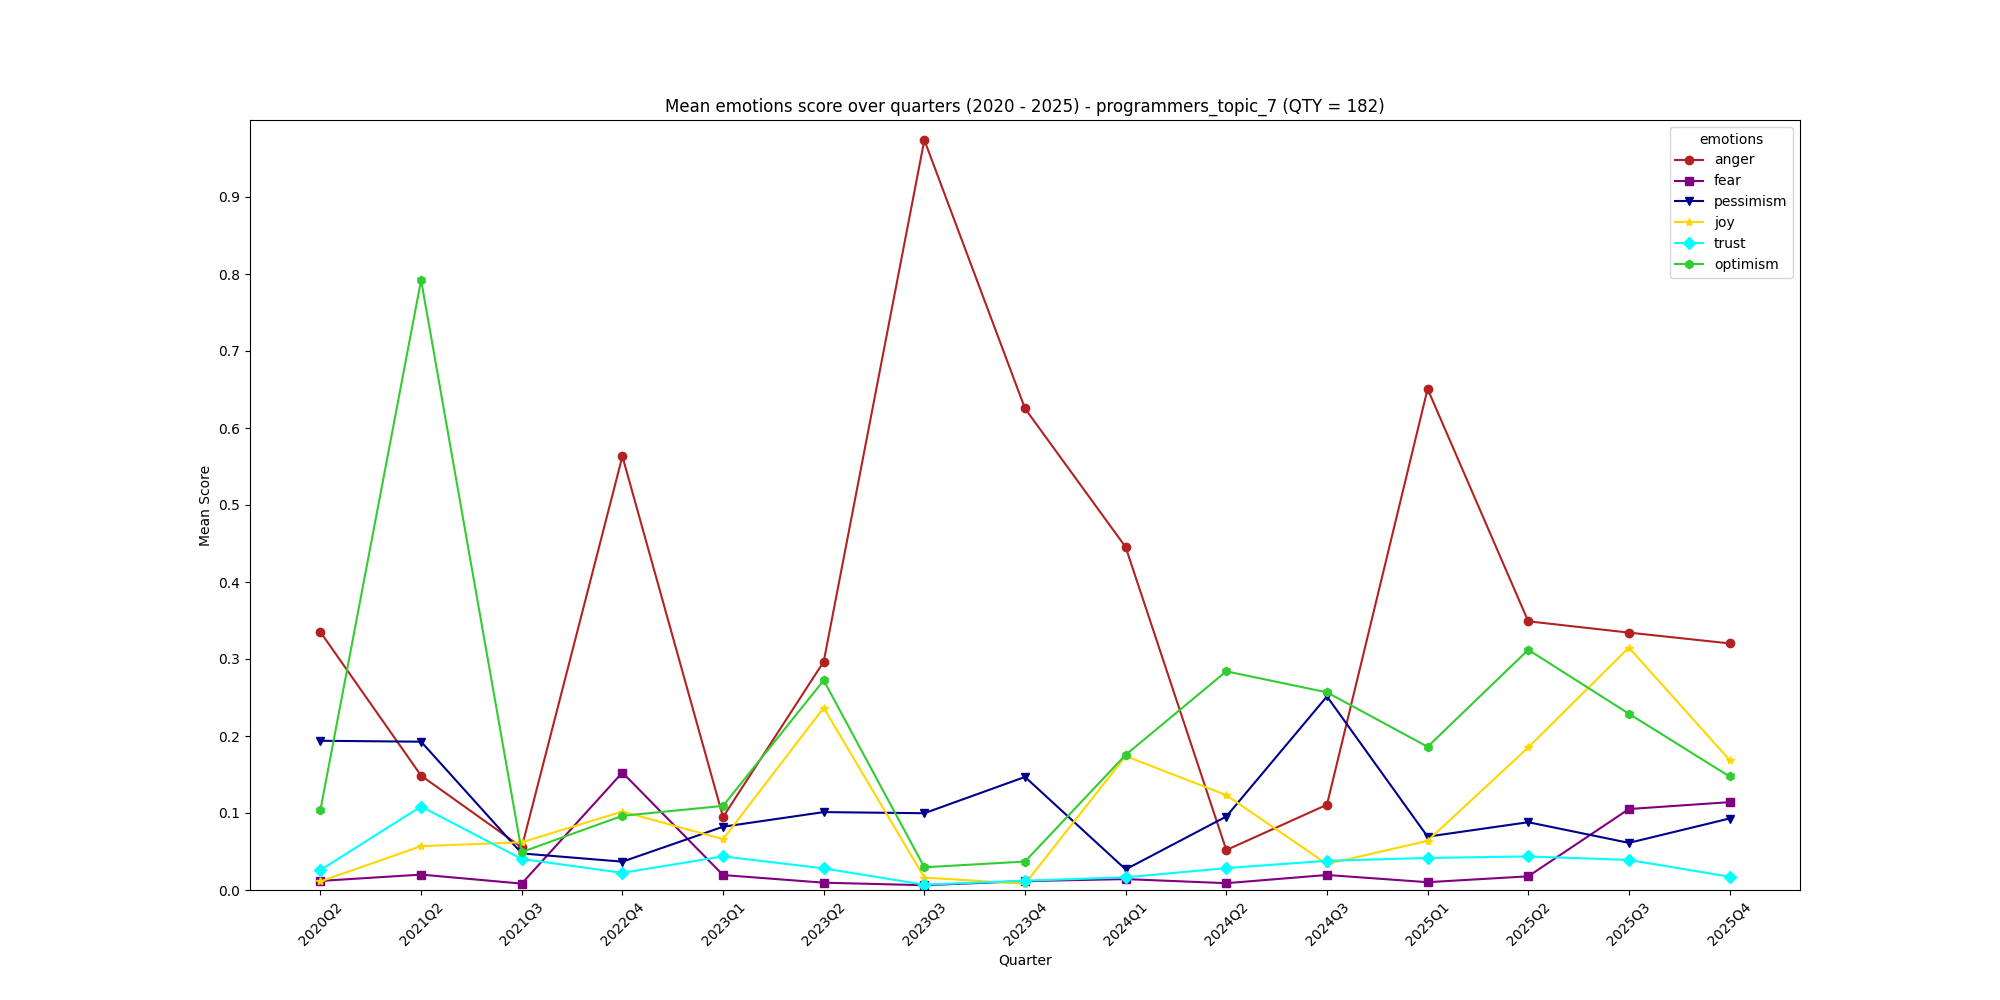
\includegraphics[width=0.80\linewidth]{Images/Appendices/Emotion/BERTopic/programmers_topic_7_emotions.png}
    \caption{Programmers topic 7}
\end{figure}
\begin{figure}[H]
    \centering
    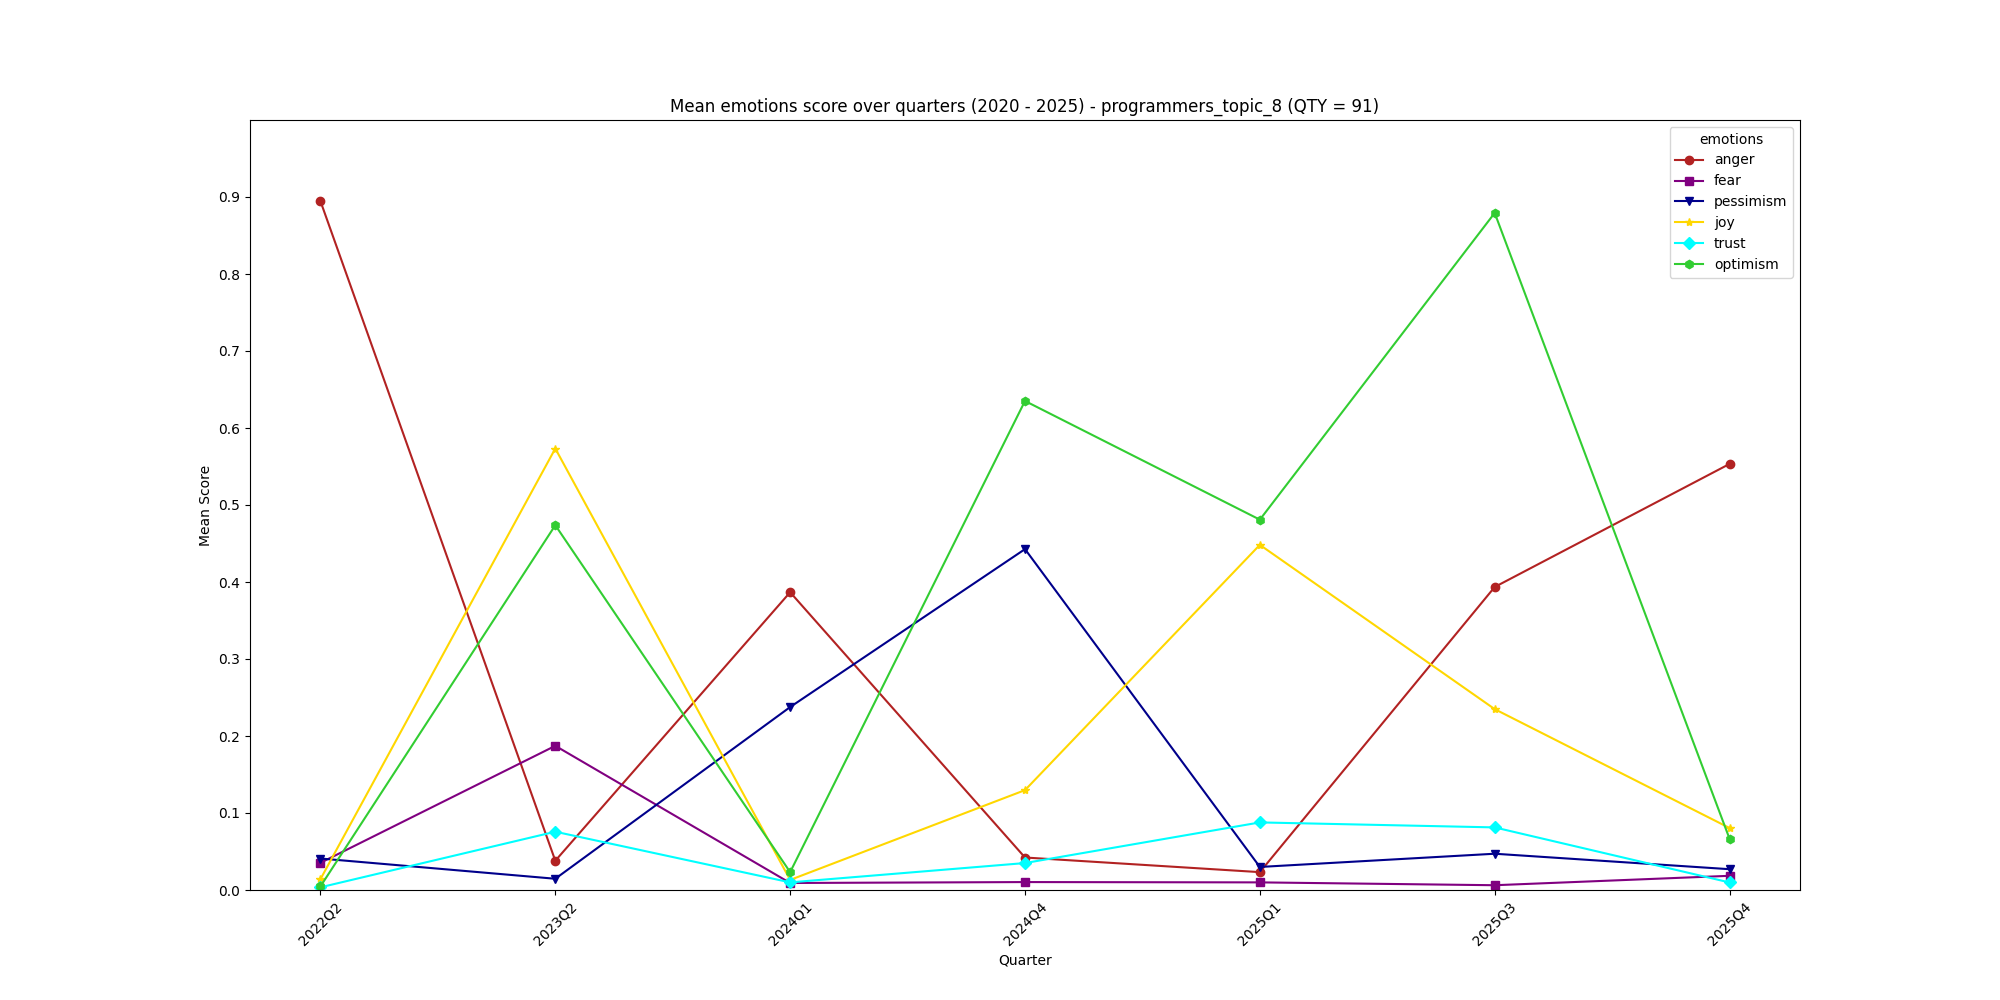
\includegraphics[width=0.80\linewidth]{Images/Appendices/Emotion/BERTopic/programmers_topic_8_emotions.png}
    \caption{Programmers topic 8}
\end{figure}
\begin{figure}[H]
    \centering
    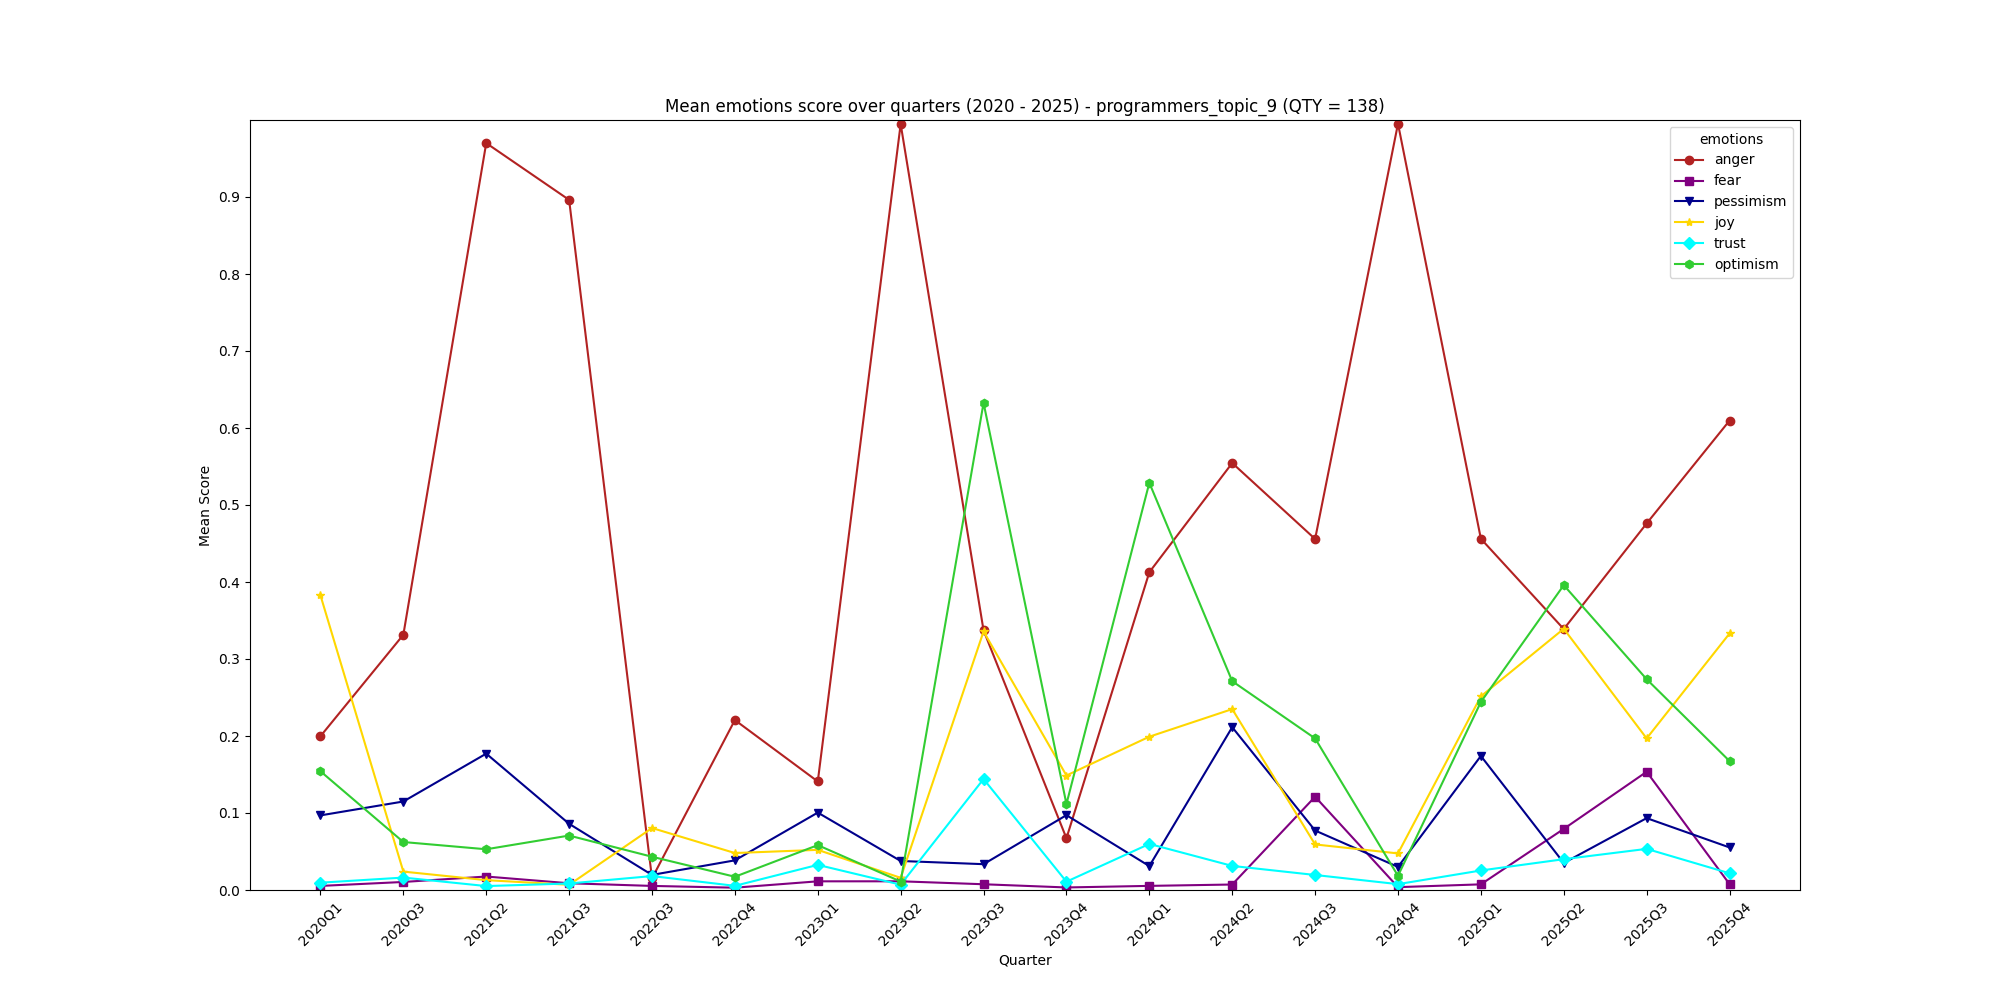
\includegraphics[width=0.80\linewidth]{Images/Appendices/Emotion/BERTopic/programmers_topic_9_emotions.png}
    \caption{Programmers topic 9}
\end{figure}

\subsection{Louvain}

\begin{figure}[H]
    \centering
    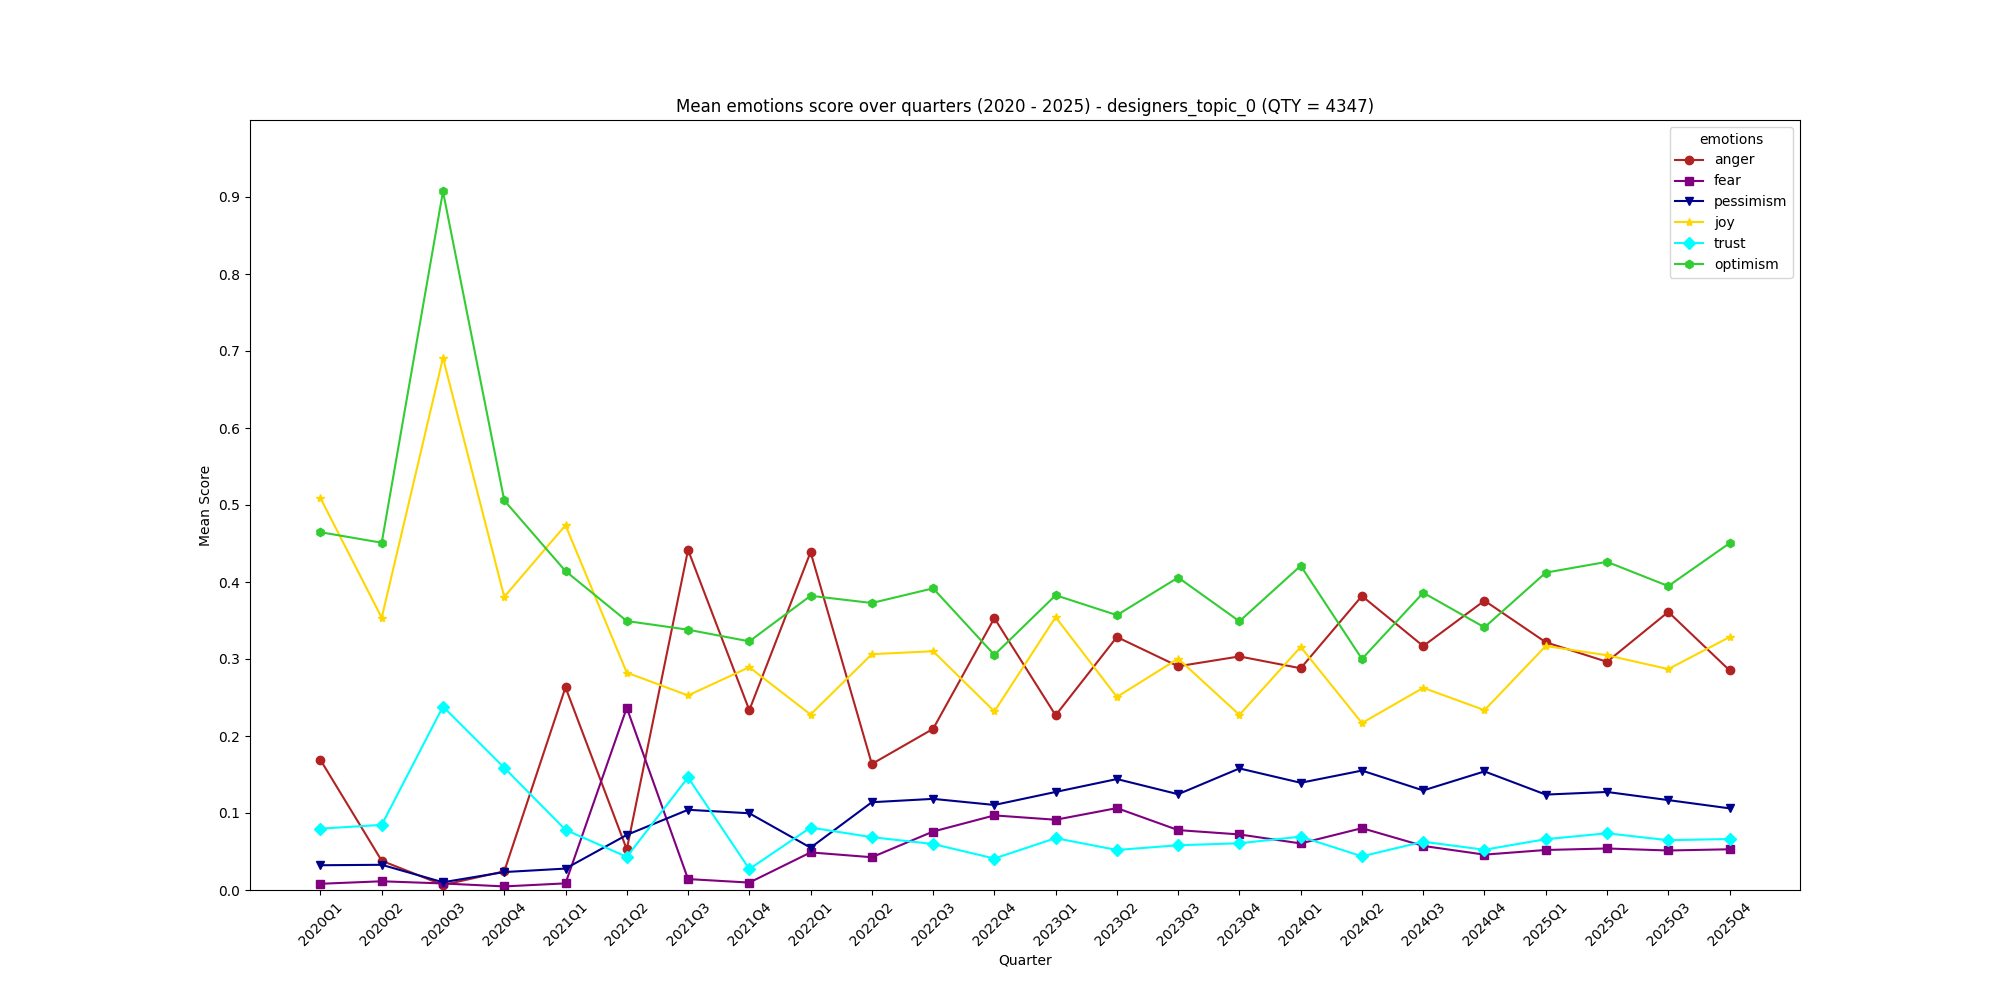
\includegraphics[width=0.80\linewidth]{Images/Appendices/Emotion/Louvain/designers_topic_0_emotions.png}
    \caption{Designers topic 0}
\end{figure}
\begin{figure}[H]
    \centering
    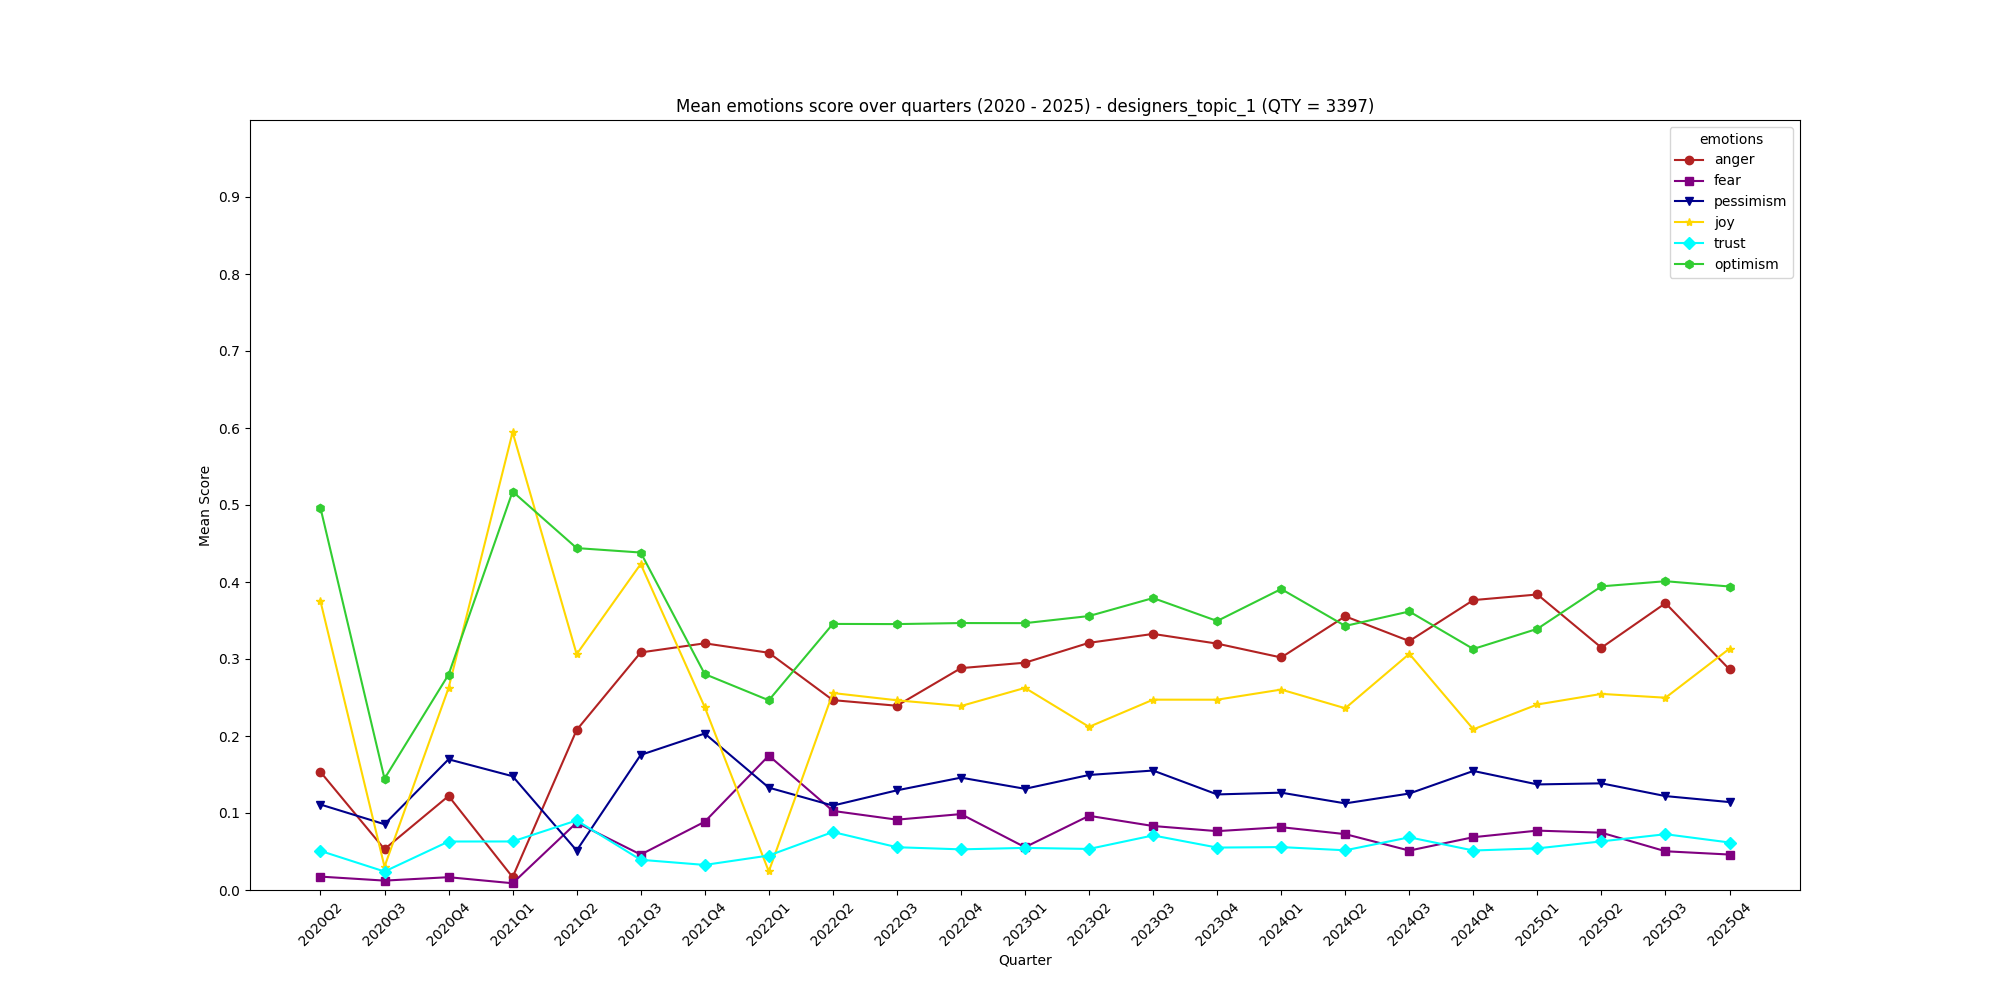
\includegraphics[width=0.80\linewidth]{Images/Appendices/Emotion/Louvain/designers_topic_1_emotions.png}
    \caption{Designers topic 1}
\end{figure}
\begin{figure}[H]
    \centering
    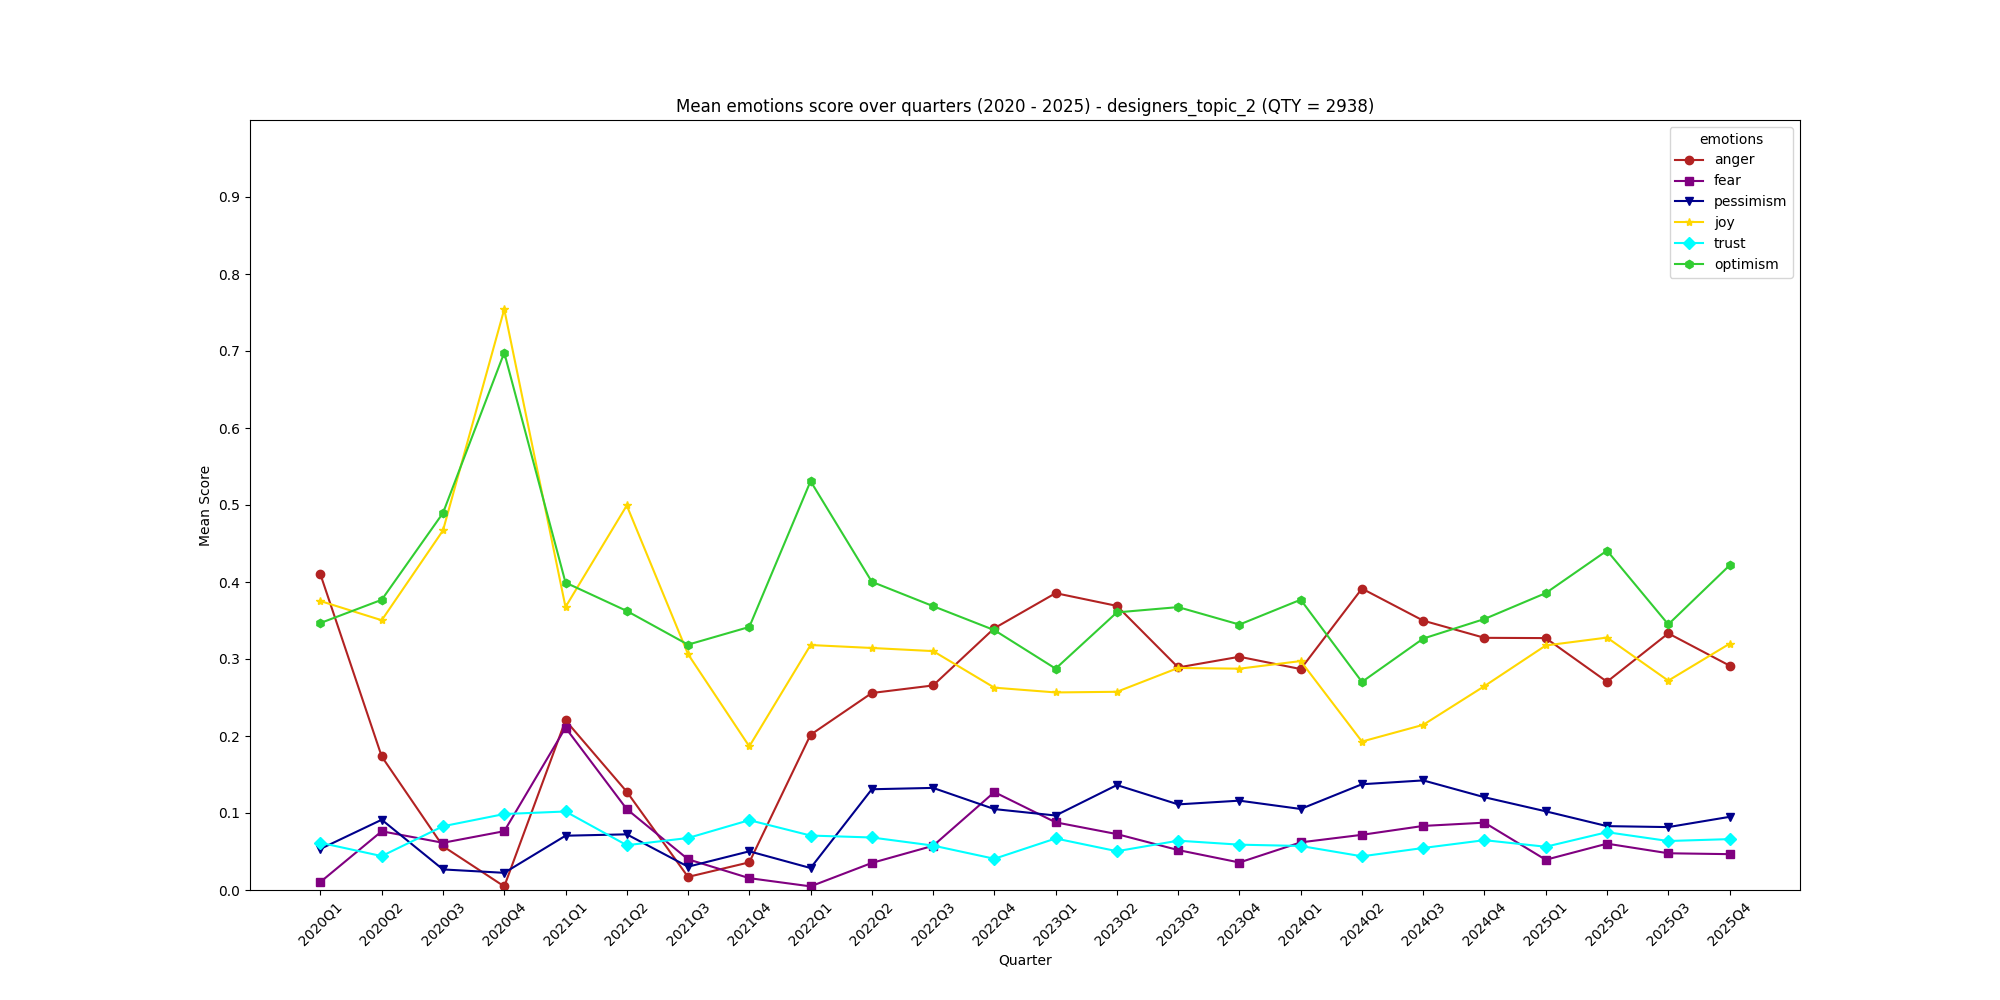
\includegraphics[width=0.80\linewidth]{Images/Appendices/Emotion/Louvain/designers_topic_2_emotions.png}
    \caption{Designers topic 2}
\end{figure}
\begin{figure}[H]
    \centering
    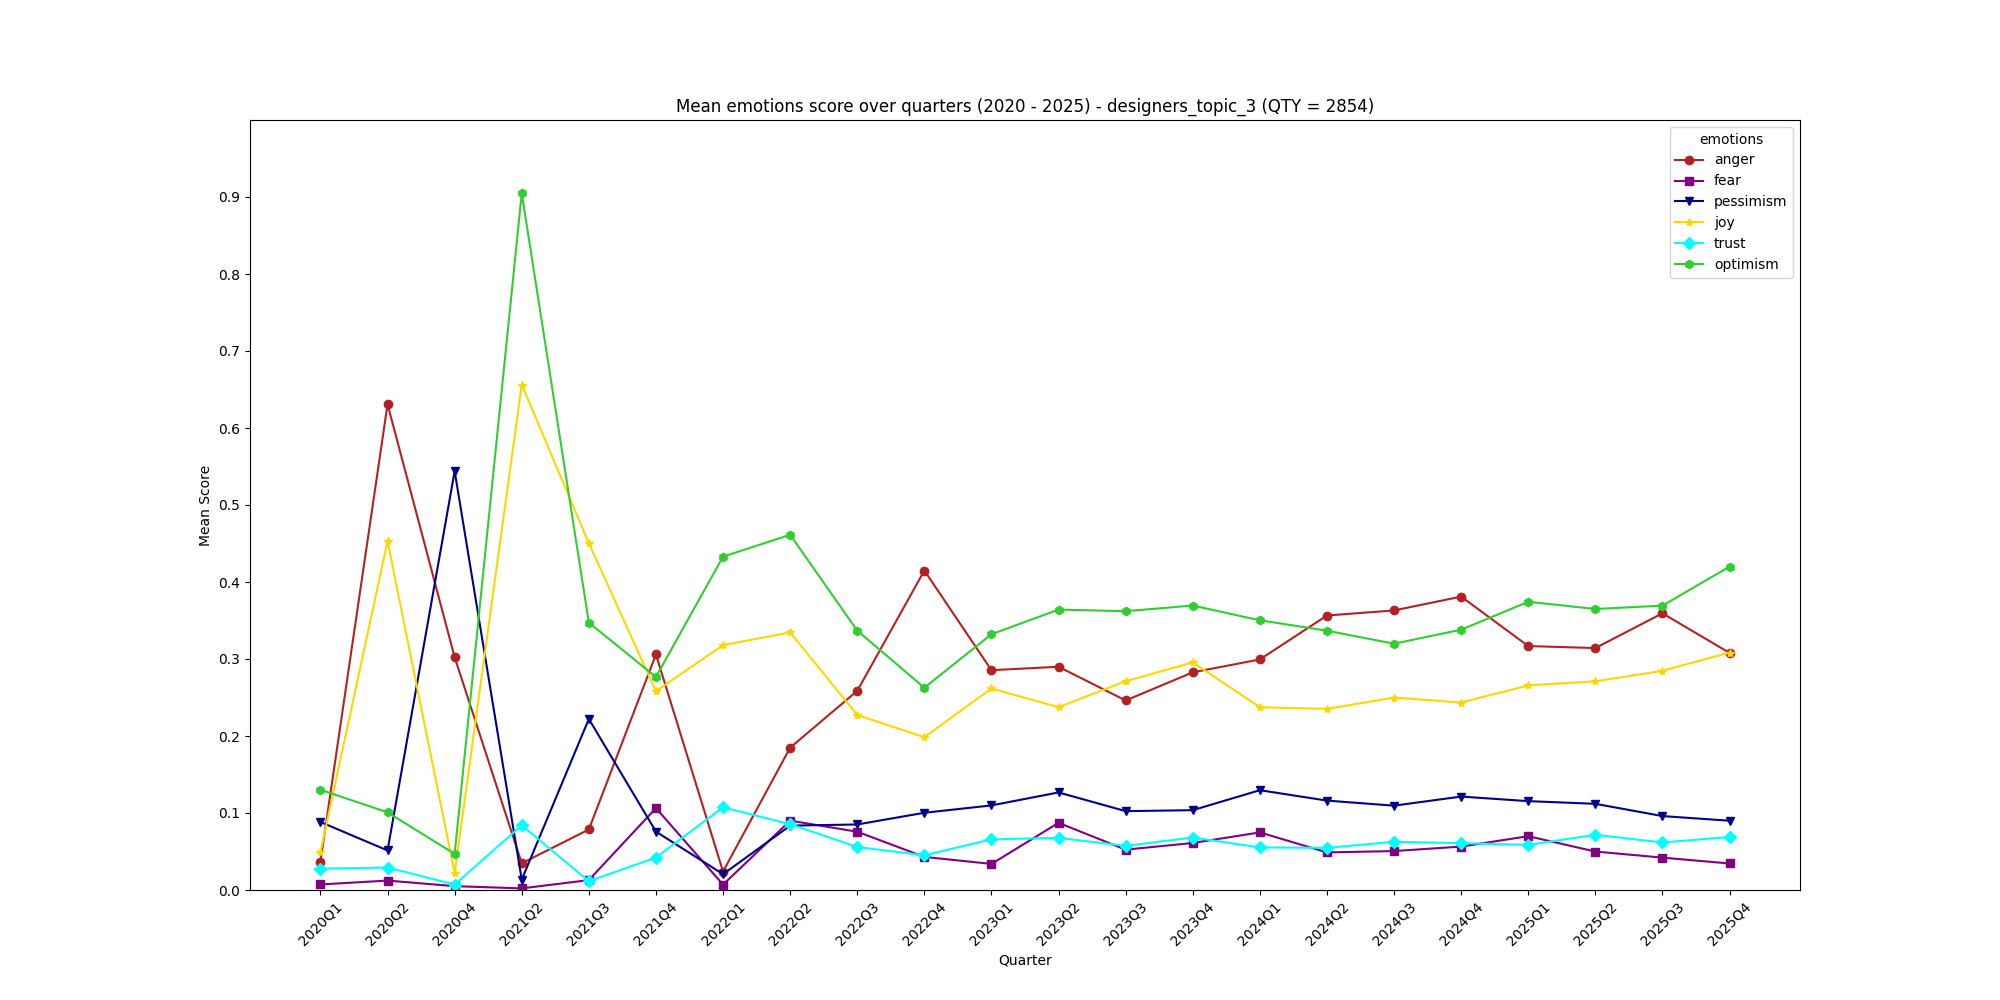
\includegraphics[width=0.80\linewidth]{Images/Appendices/Emotion/Louvain/designers_topic_3_emotions.png}
    \caption{Designers topic 3}
\end{figure}
\begin{figure}[H]
    \centering
    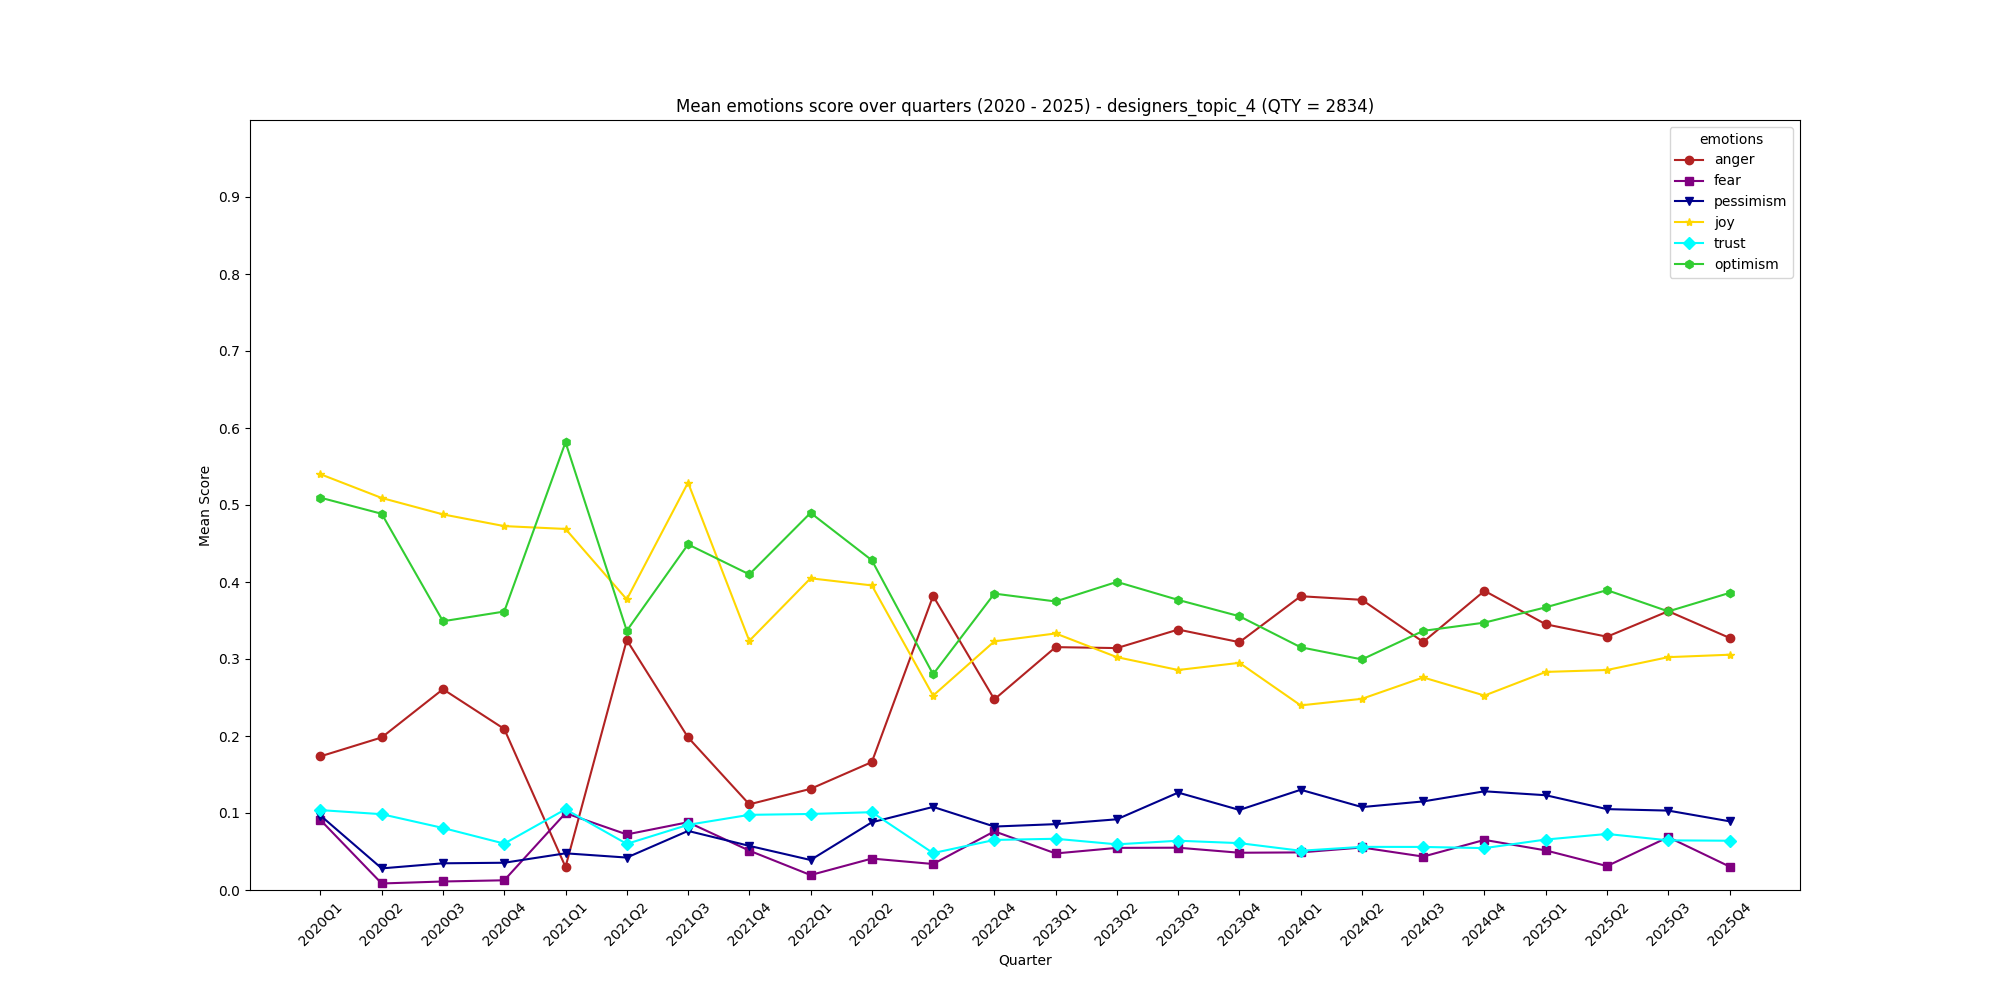
\includegraphics[width=0.80\linewidth]{Images/Appendices/Emotion/Louvain/designers_topic_4_emotions.png}
    \caption{Designers topic 4}
\end{figure}
\begin{figure}[H]
    \centering
    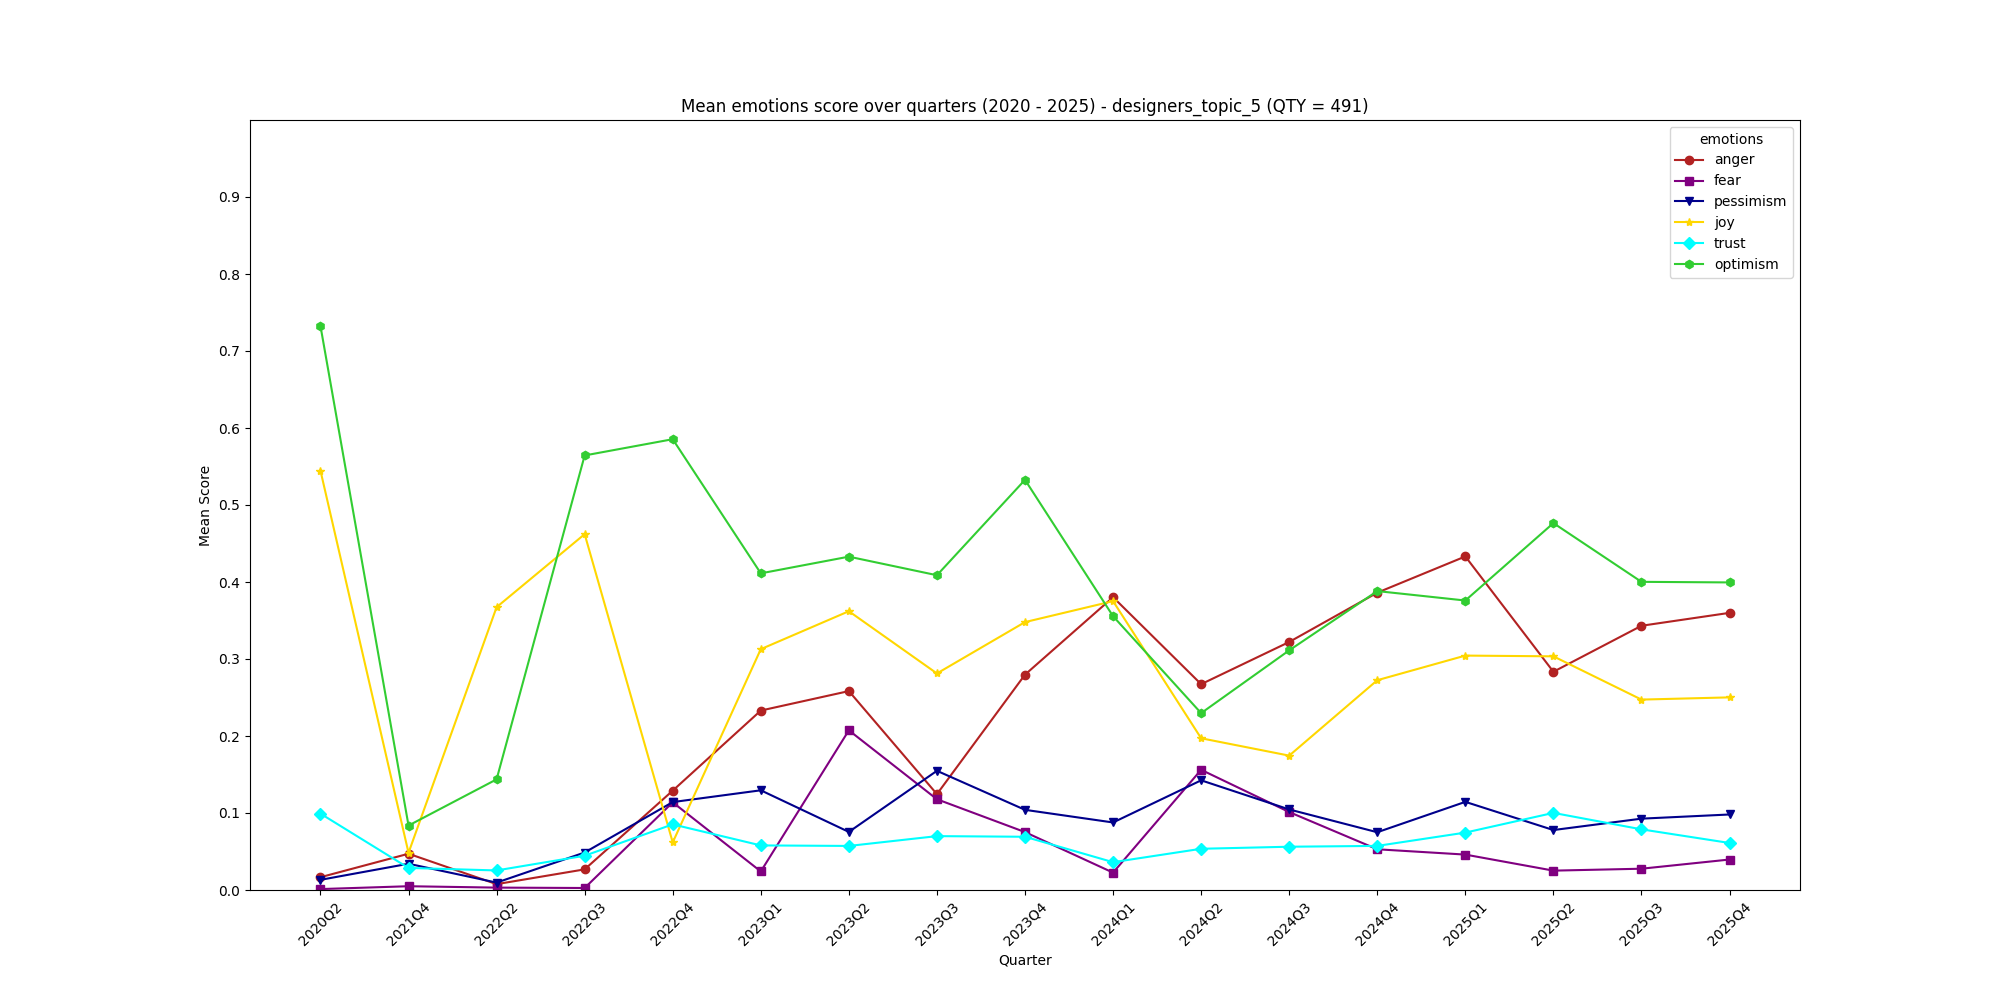
\includegraphics[width=0.80\linewidth]{Images/Appendices/Emotion/Louvain/designers_topic_5_emotions.png}
    \caption{Designers topic 5}
\end{figure}
\begin{figure}[H]
    \centering
    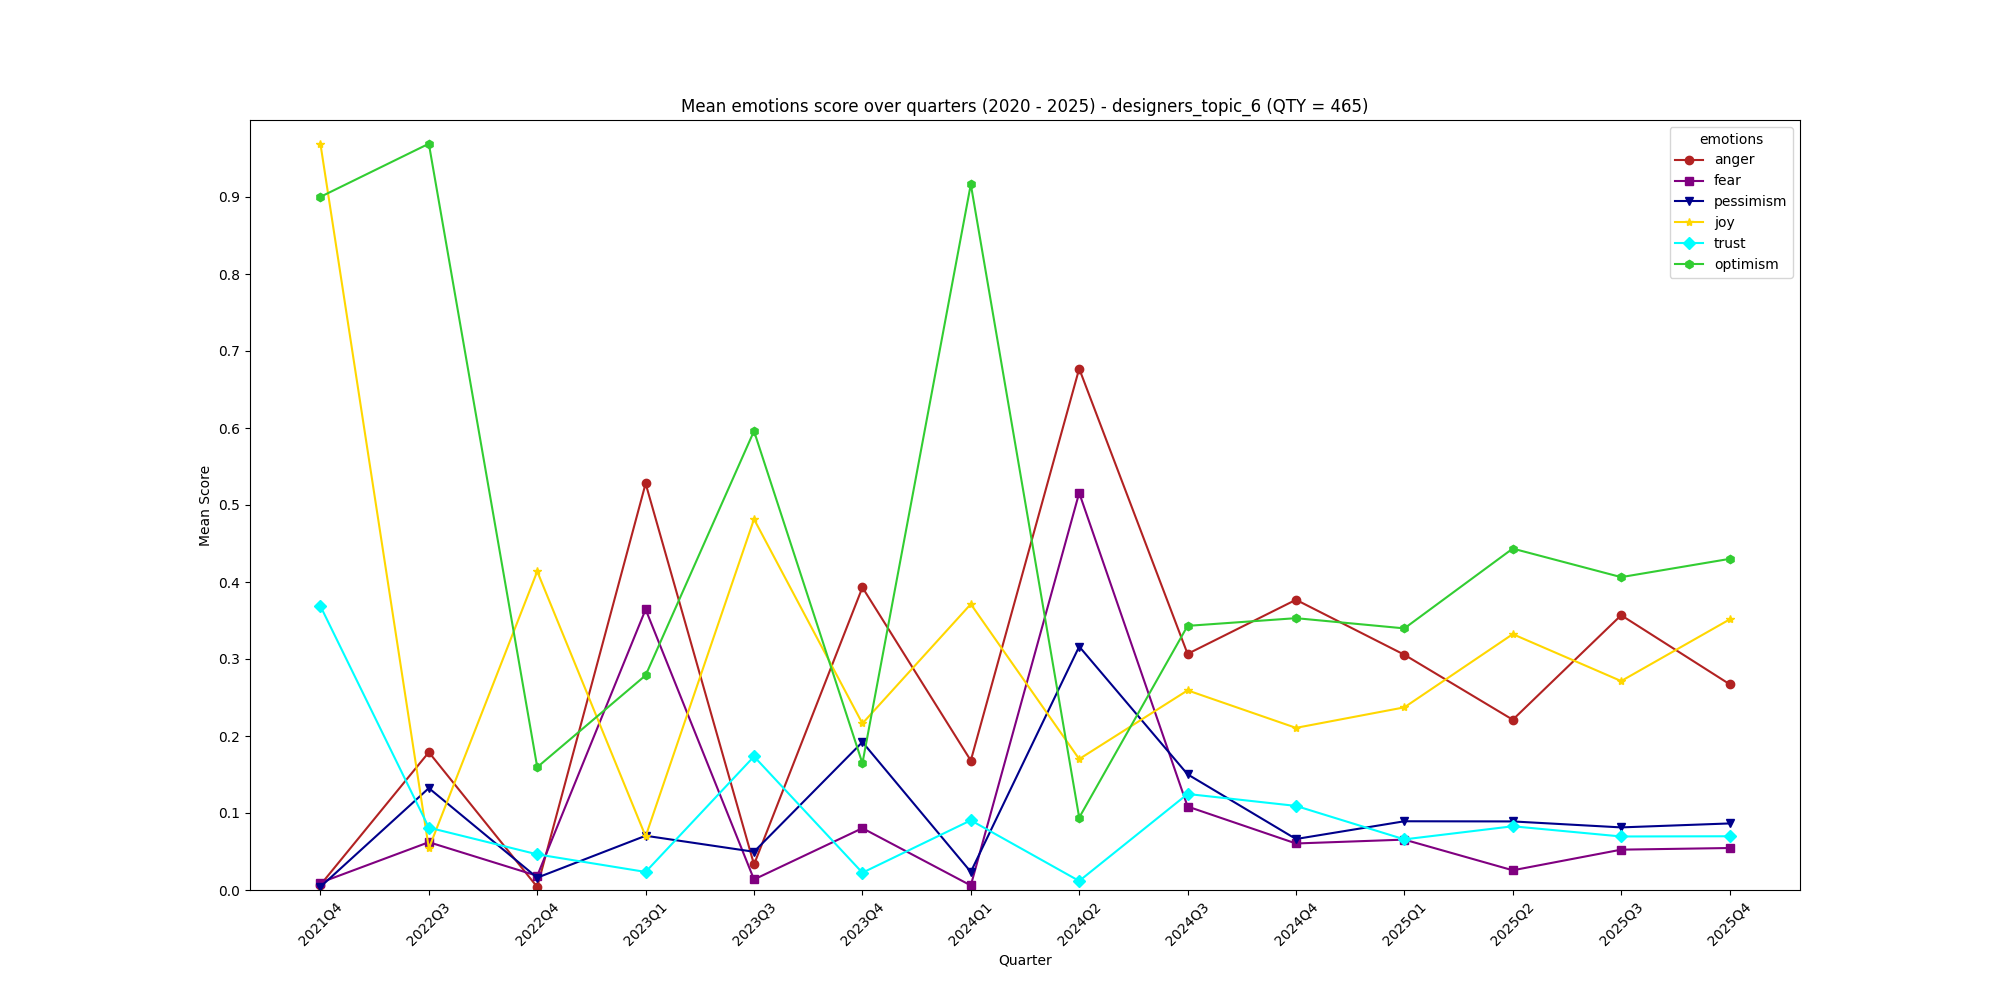
\includegraphics[width=0.80\linewidth]{Images/Appendices/Emotion/Louvain/designers_topic_6_emotions.png}
    \caption{Designers topic 6}
\end{figure}

\begin{figure}[H]
    \centering
    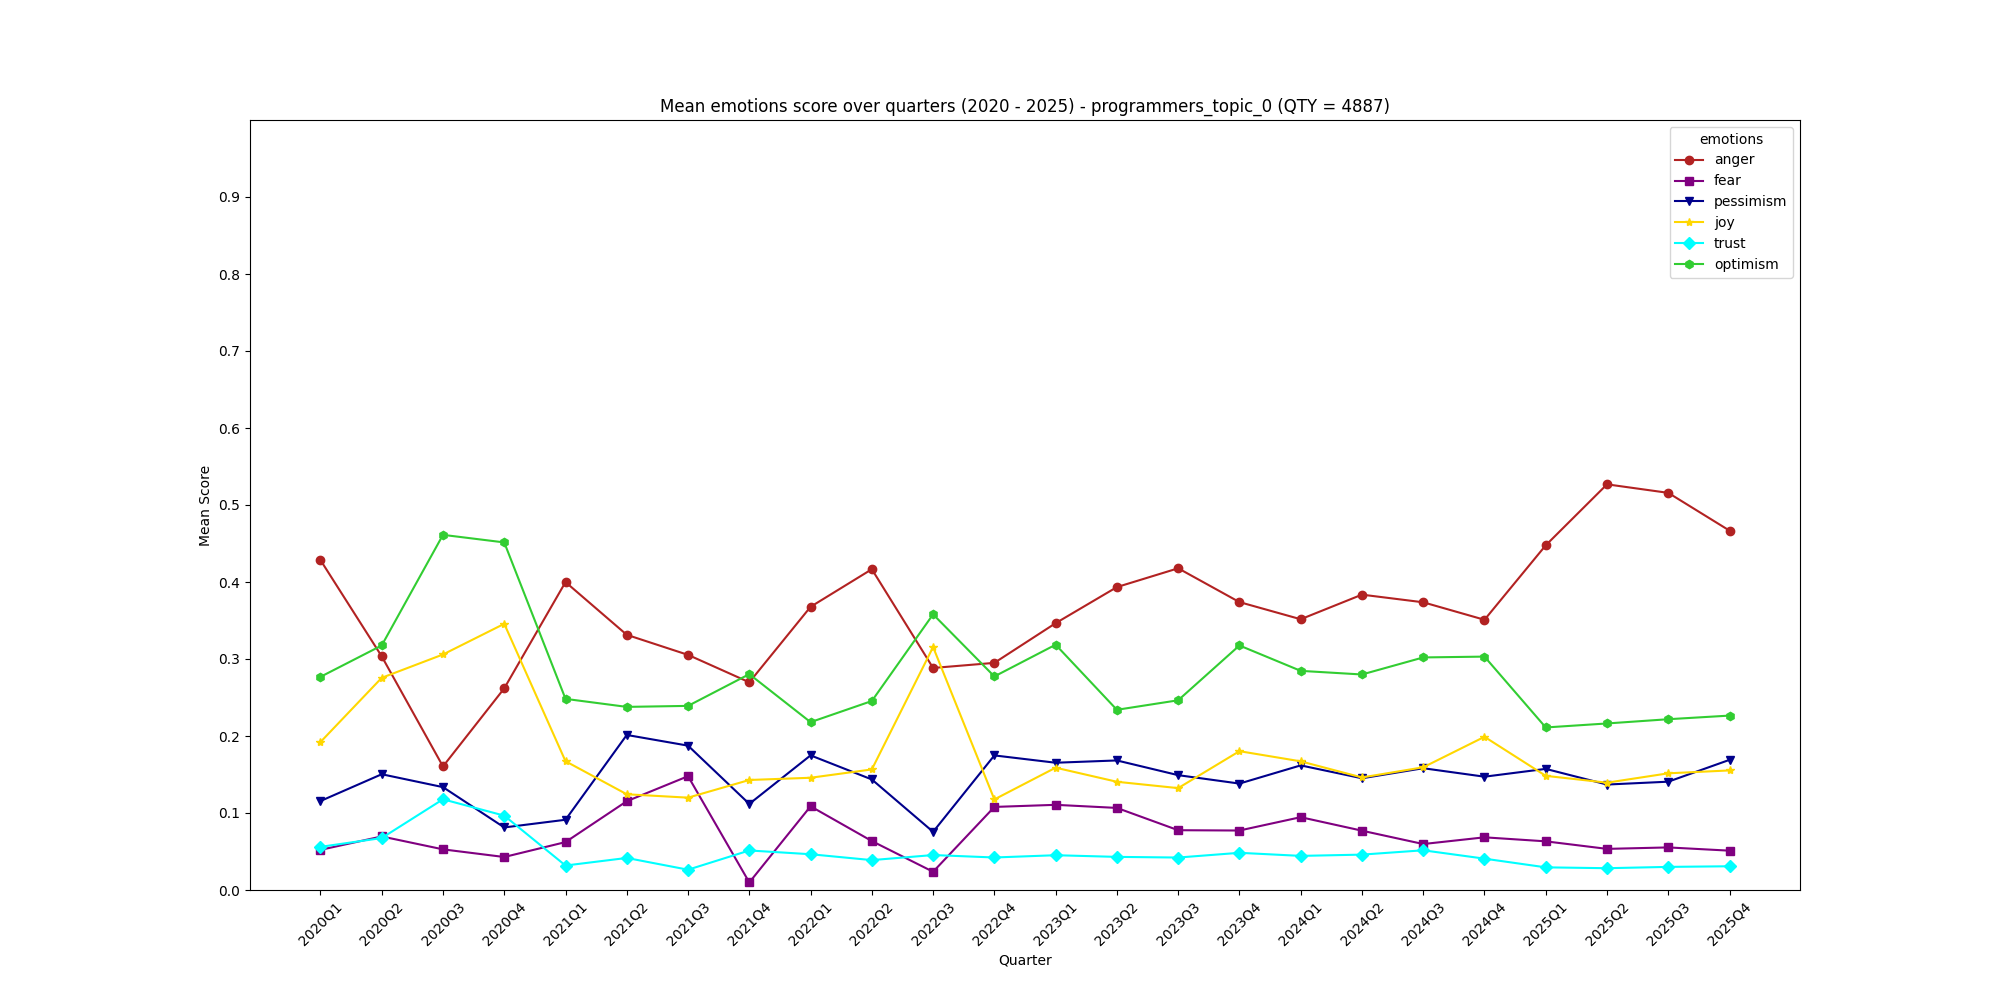
\includegraphics[width=0.80\linewidth]{Images/Appendices/Emotion/Louvain/programmers_topic_0_emotions.png}
    \caption{Programmers topic 0}
\end{figure}
\begin{figure}[H]
    \centering
    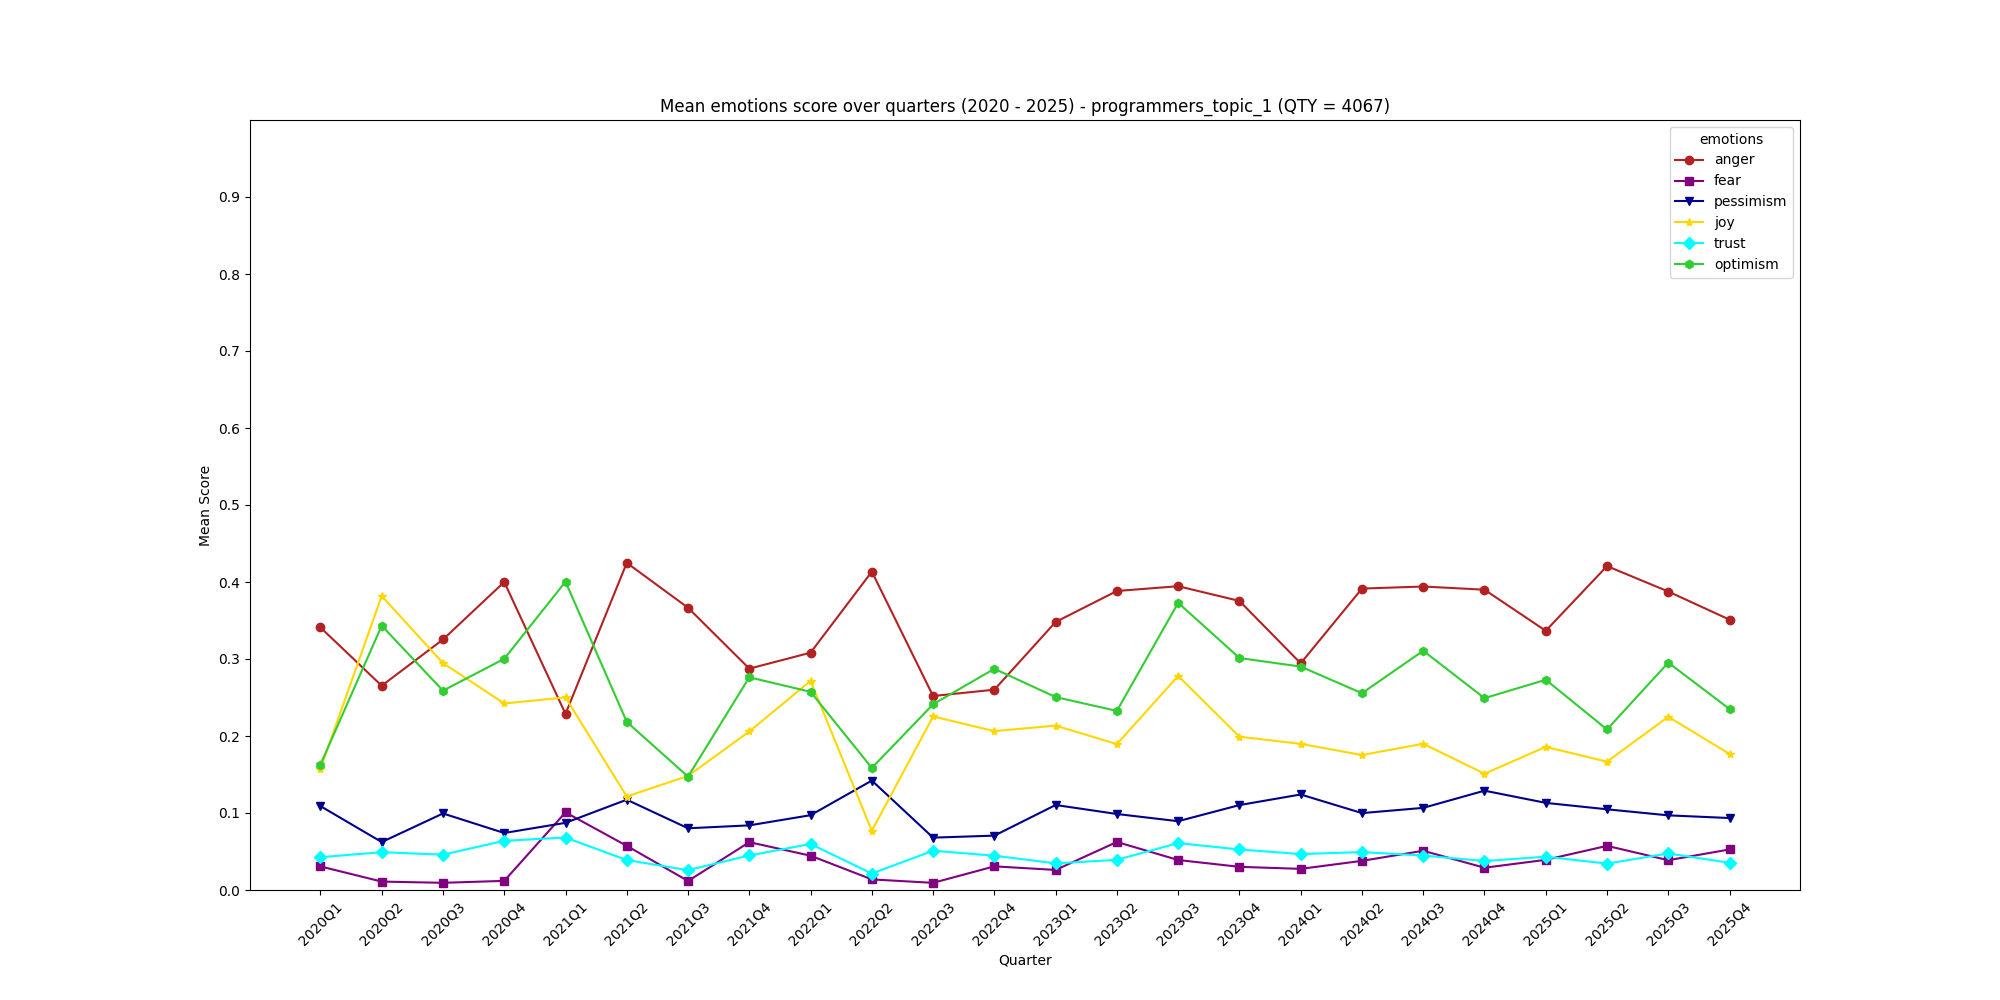
\includegraphics[width=0.80\linewidth]{Images/Appendices/Emotion/Louvain/programmers_topic_1_emotions.png}
    \caption{Programmers topic 1}
\end{figure}
\begin{figure}[H]
    \centering
    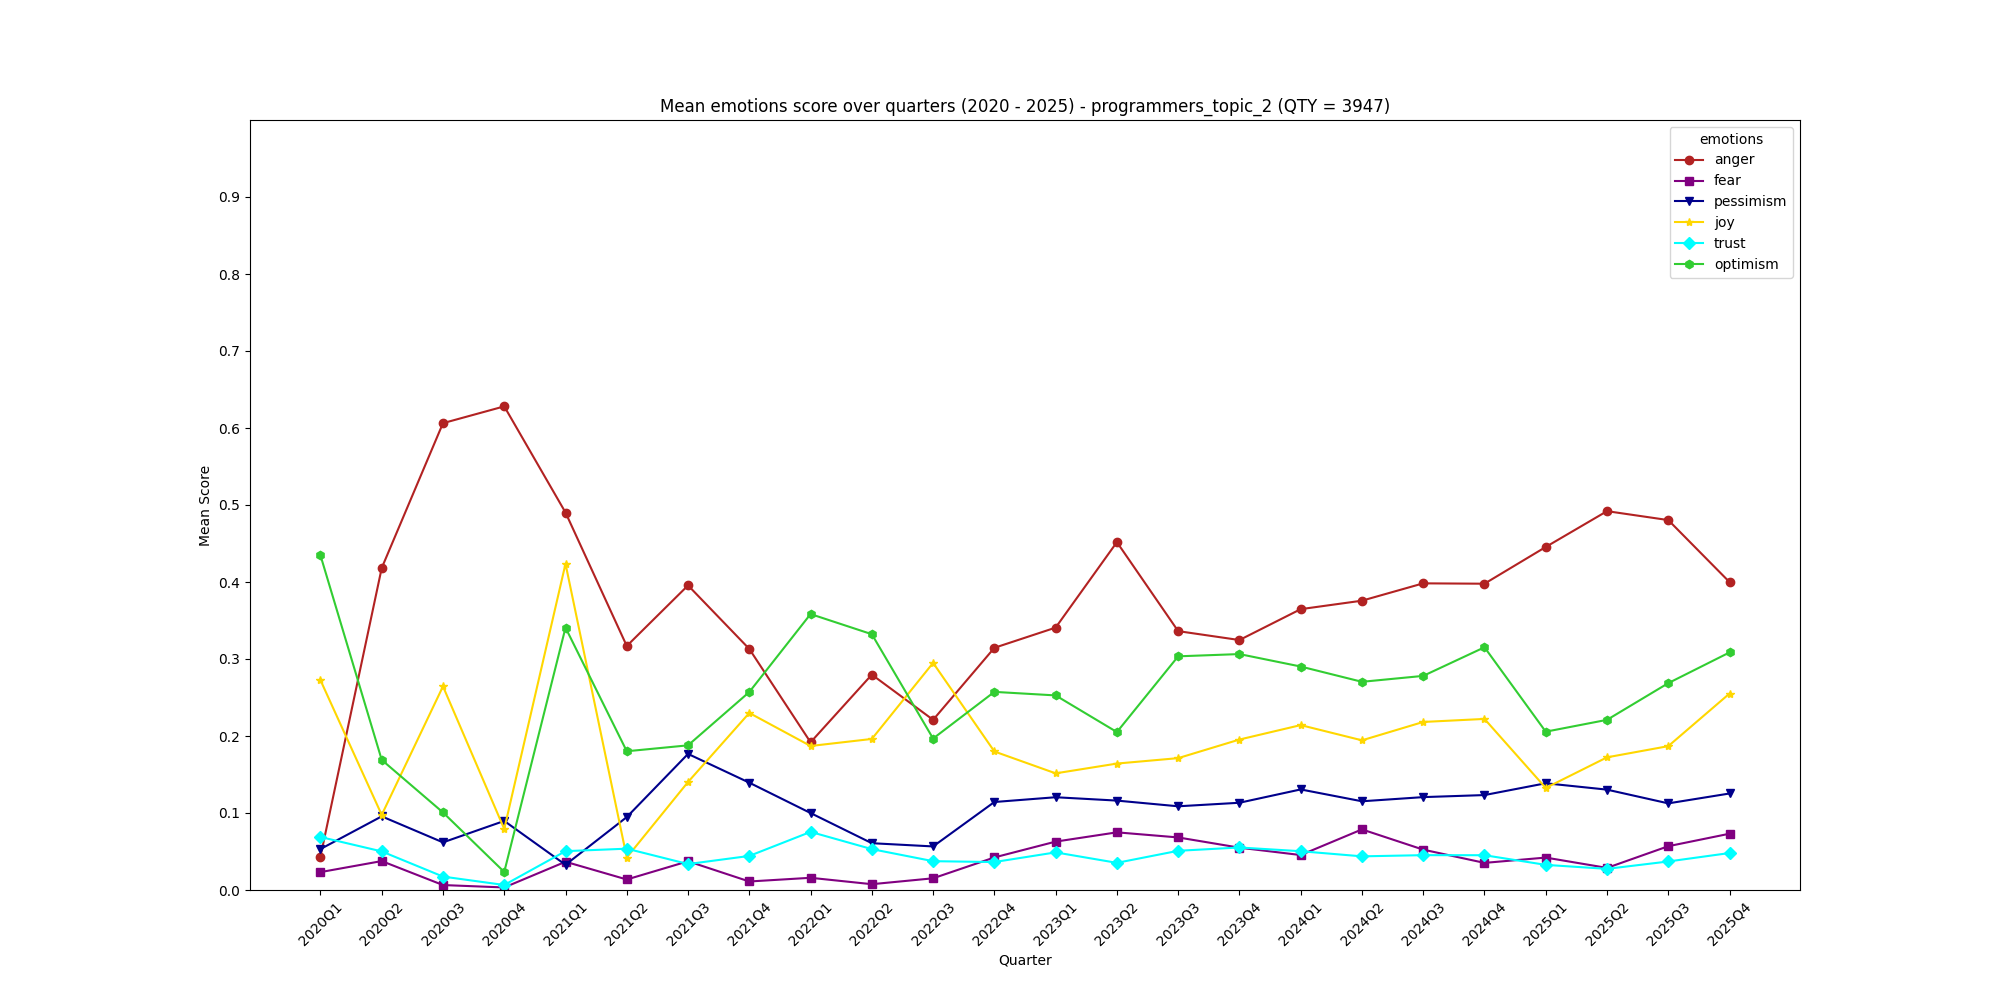
\includegraphics[width=0.80\linewidth]{Images/Appendices/Emotion/Louvain/programmers_topic_2_emotions.png}
    \caption{Programmers topic 2}
\end{figure}
\begin{figure}[H]
    \centering
    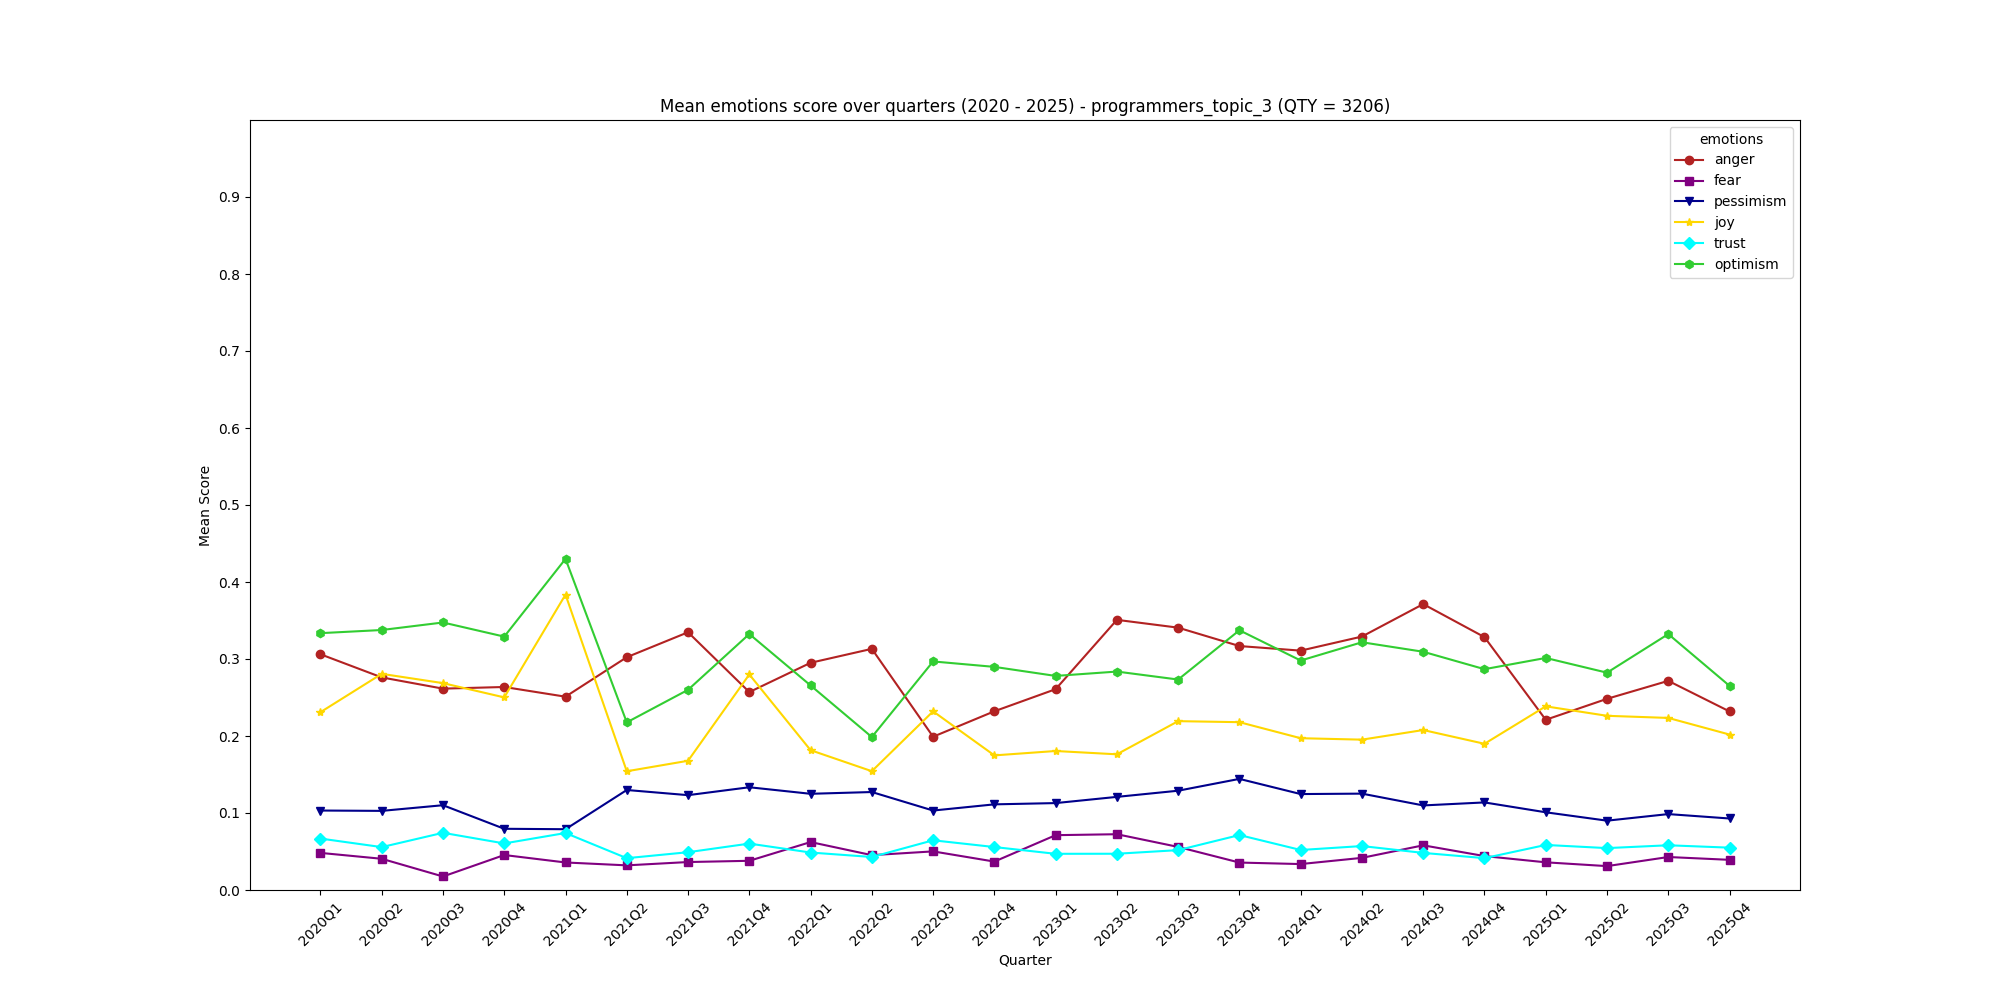
\includegraphics[width=0.80\linewidth]{Images/Appendices/Emotion/Louvain/programmers_topic_3_emotions.png}
    \caption{Programmers topic 3}
\end{figure}
\begin{figure}[H]
    \centering
    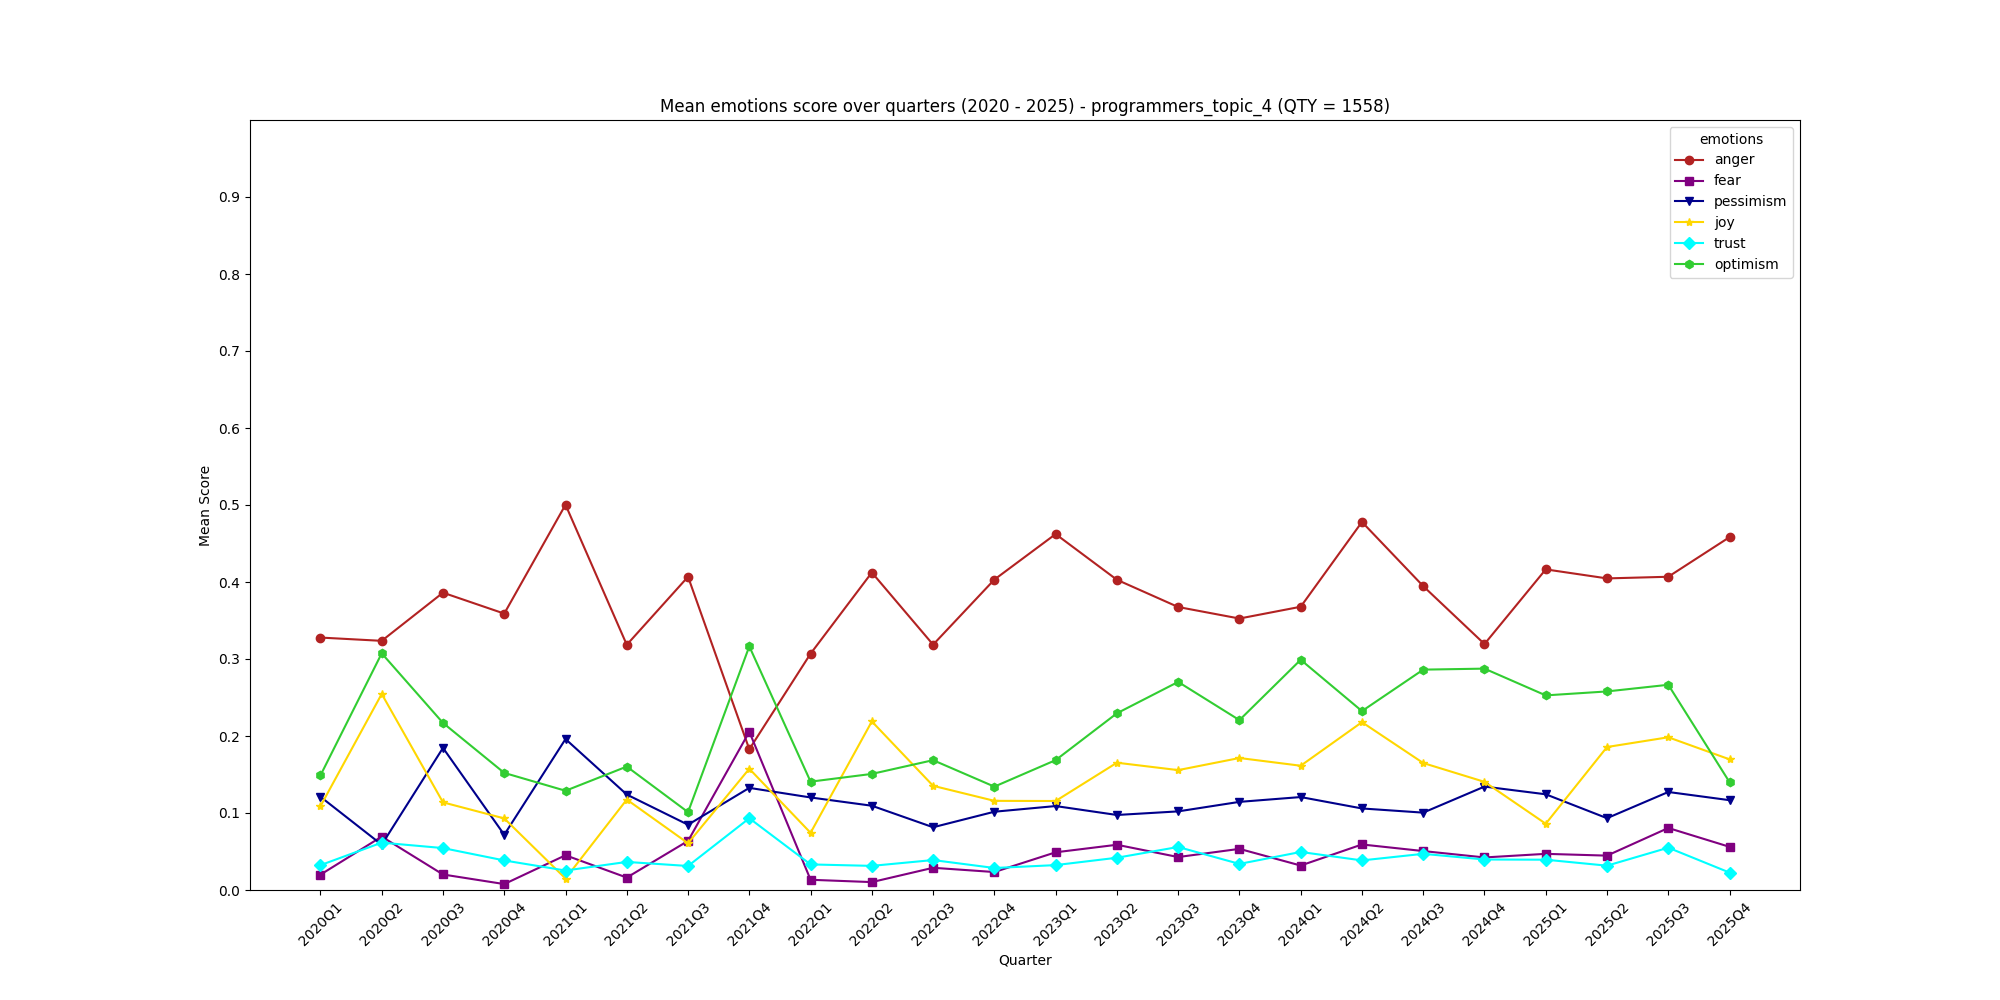
\includegraphics[width=0.80\linewidth]{Images/Appendices/Emotion/Louvain/programmers_topic_4_emotions.png}
    \caption{Programmers topic 4}
\end{figure}

\section{Sentiment analysis}

\subsection{BERTopic}
\begin{figure}[H]
    \centering
    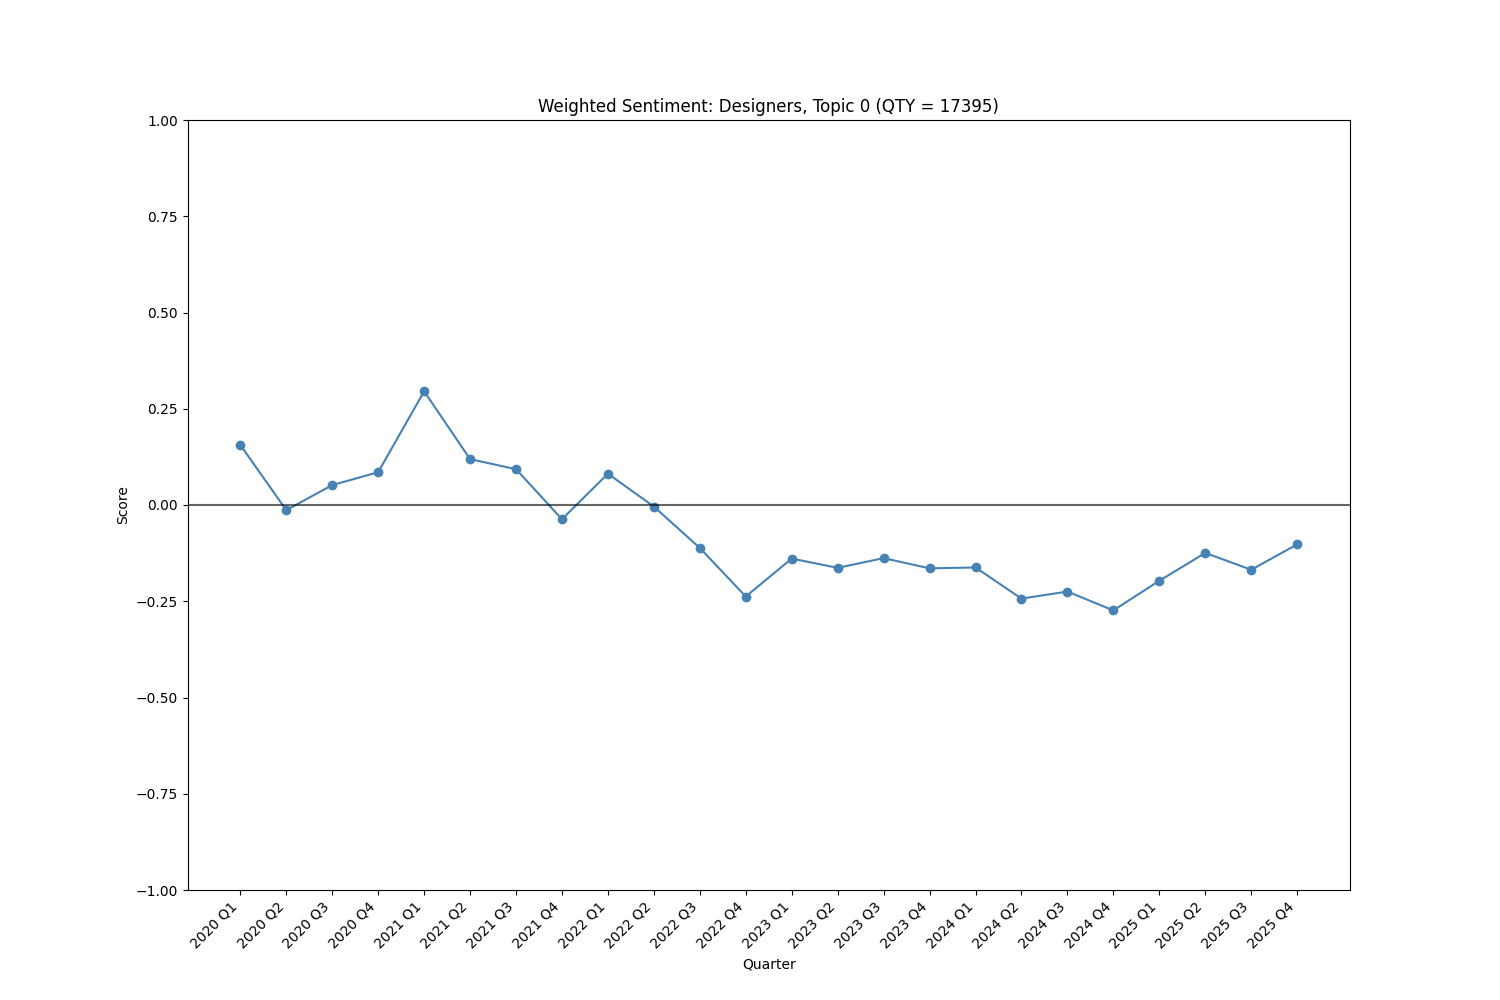
\includegraphics[width=0.80\linewidth]{Images/Appendices/Sentiment/BERTopic/designers_bert_weighted_topic_0.png}
    \caption{Designers topic 0}
\end{figure}
\begin{figure}[H]
    \centering
    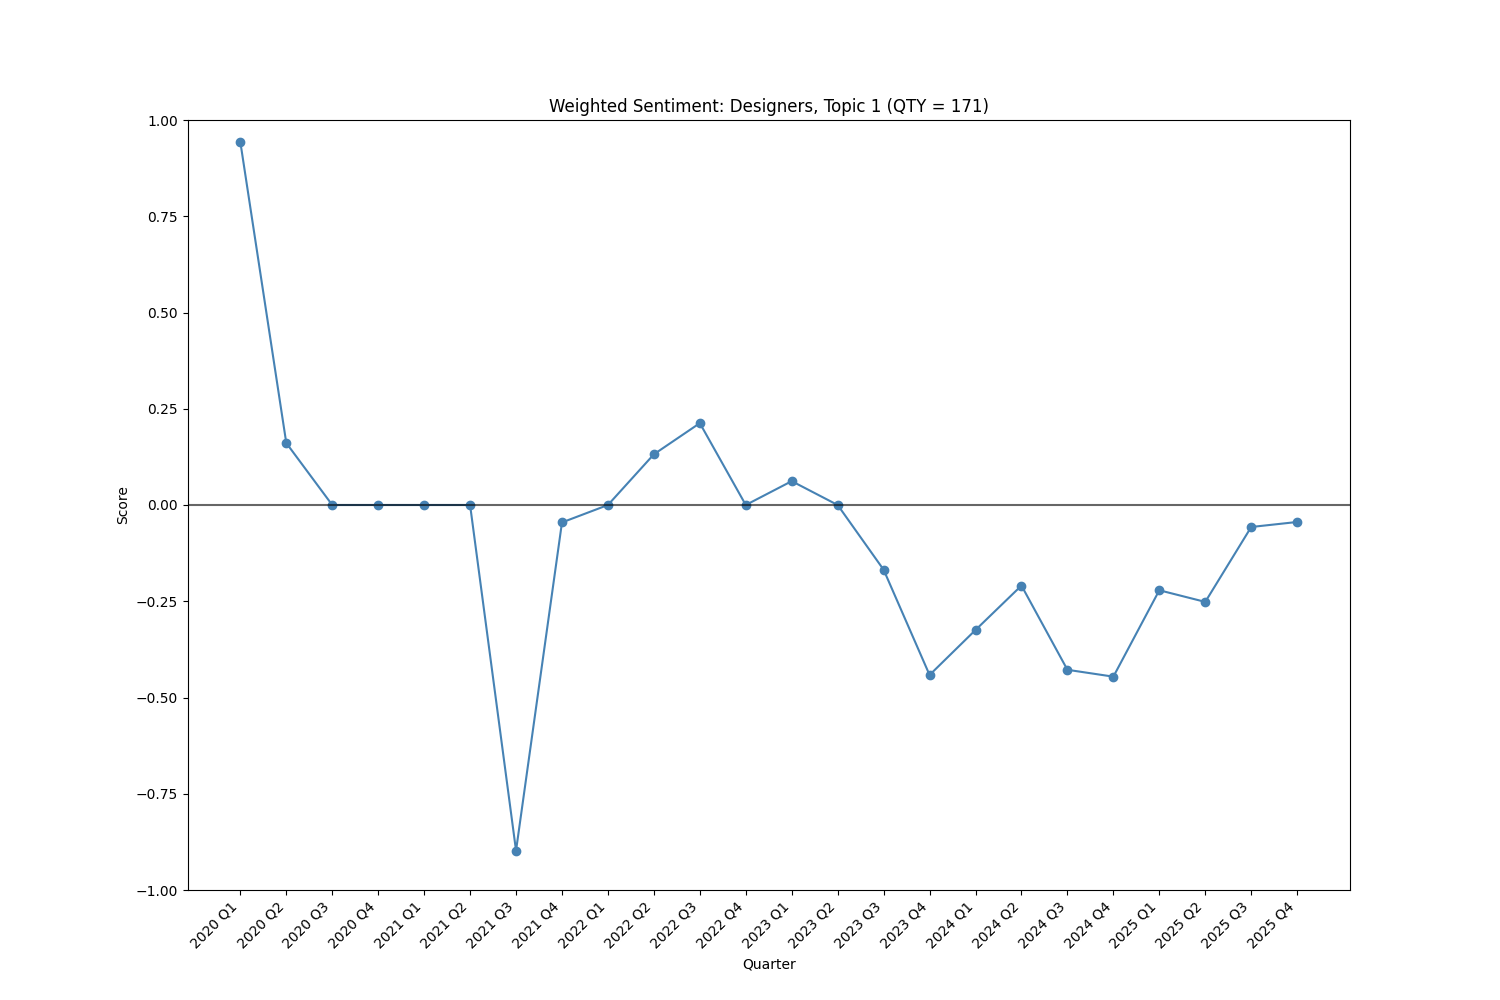
\includegraphics[width=0.80\linewidth]{Images/Appendices/Sentiment/BERTopic/designers_bert_weighted_topic_1.png}
    \caption{Designers topic 1}
\end{figure}
\begin{figure}[H]
    \centering
    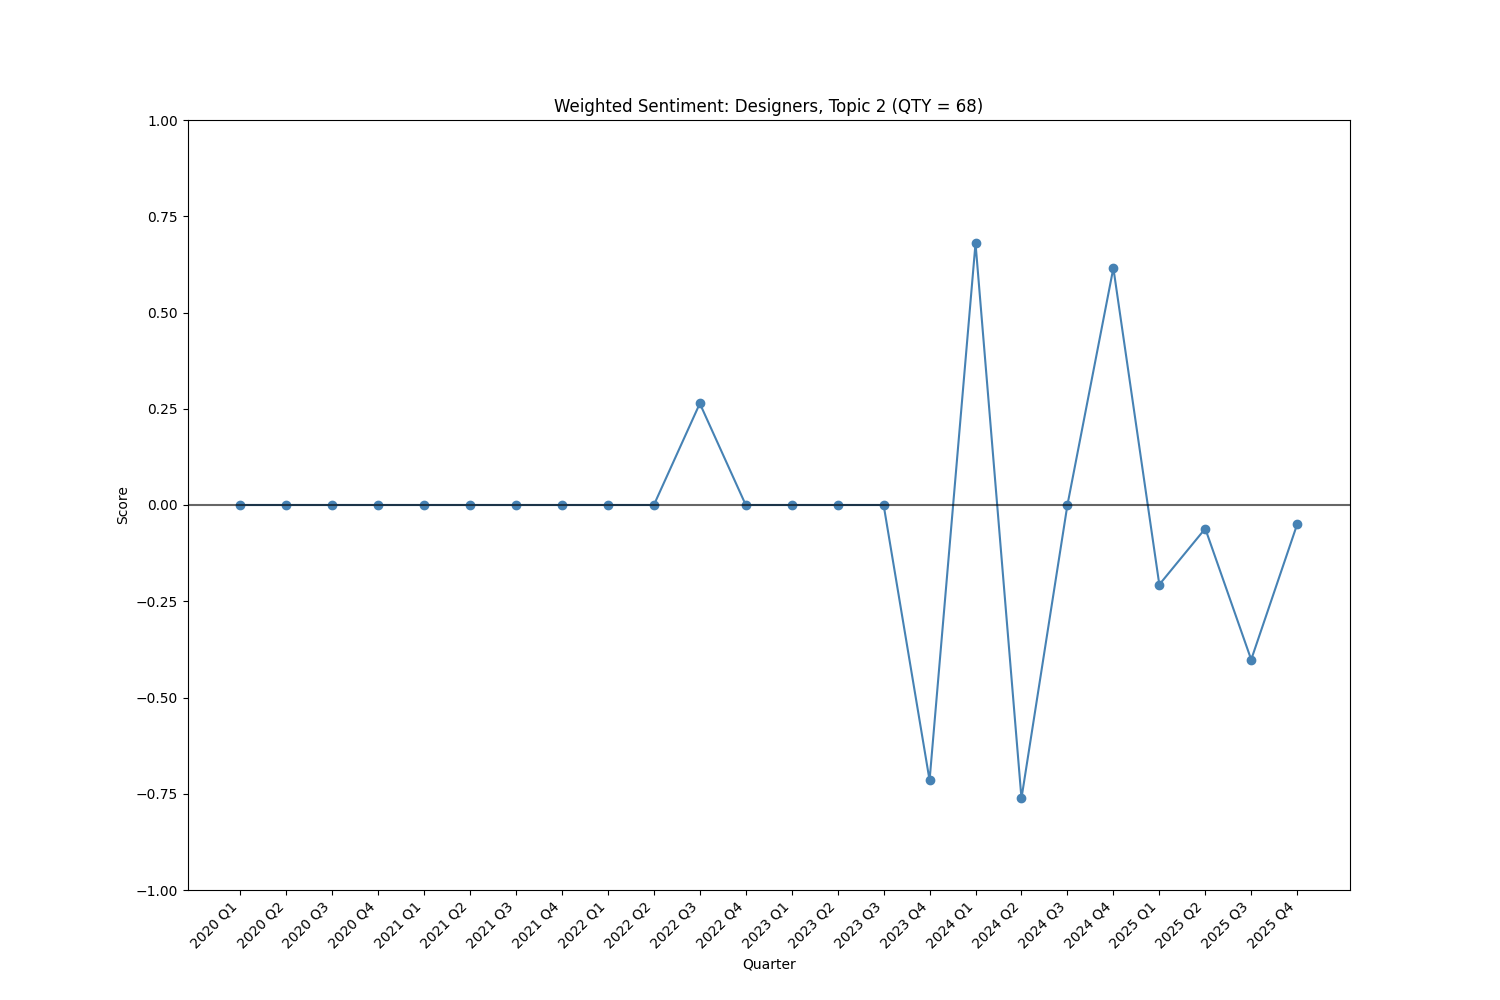
\includegraphics[width=0.80\linewidth]{Images/Appendices/Sentiment/BERTopic/designers_bert_weighted_topic_2.png}
    \caption{Designers topic 2}
\end{figure}
\begin{figure}[H]
    \centering
    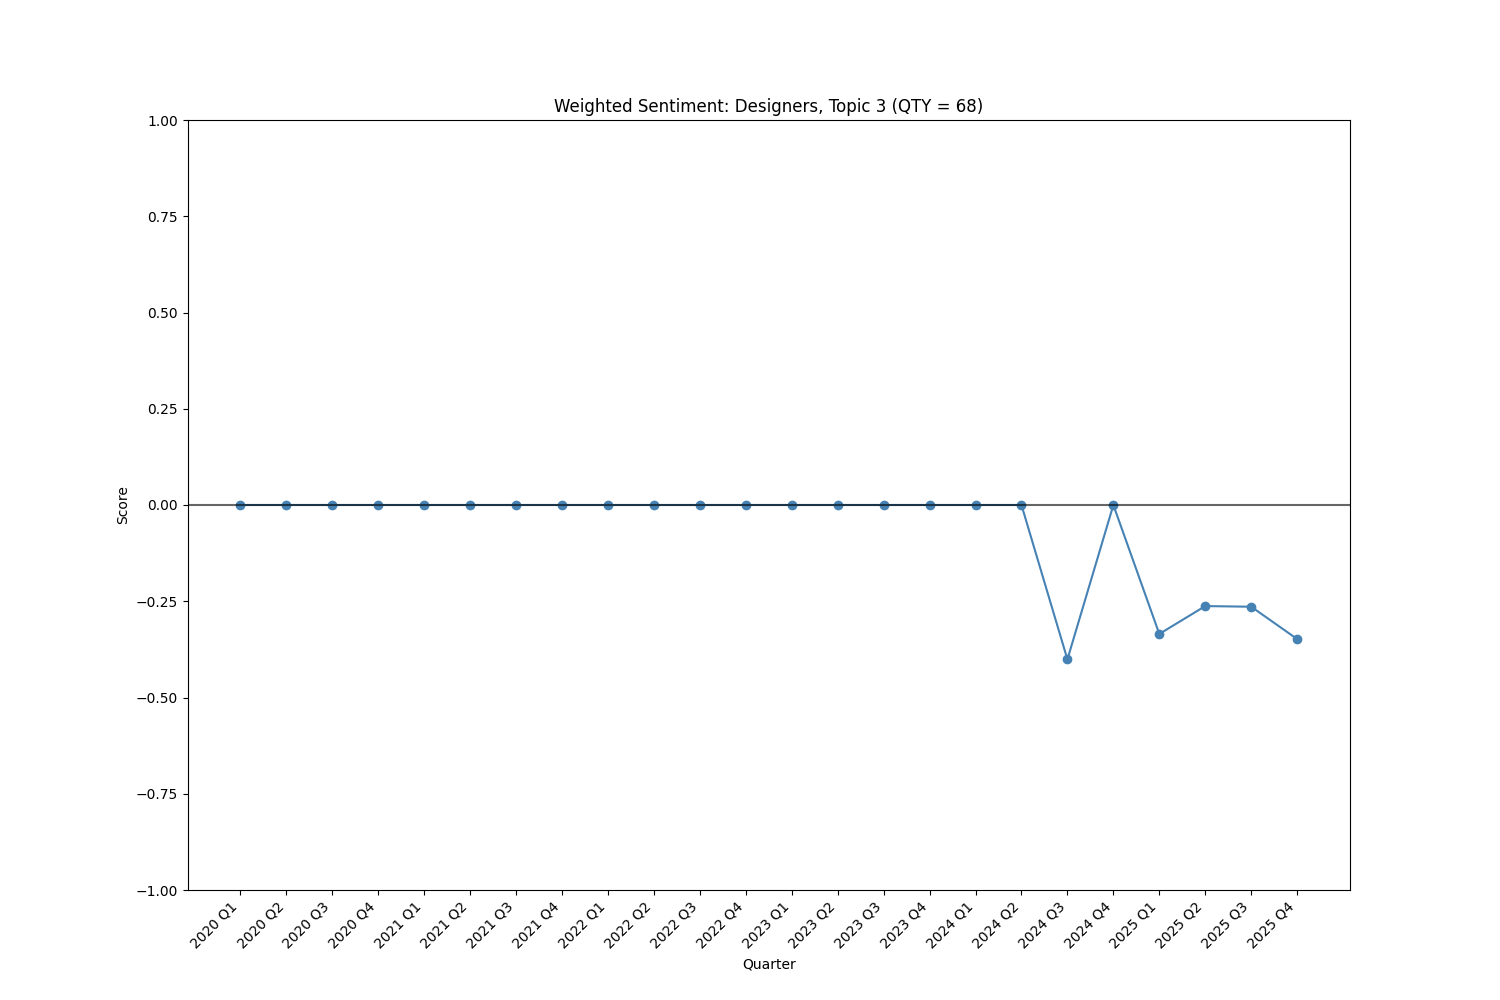
\includegraphics[width=0.80\linewidth]{Images/Appendices/Sentiment/BERTopic/designers_bert_weighted_topic_3.png}
    \caption{Designers topic 3}
\end{figure}
\begin{figure}[H]
    \centering
    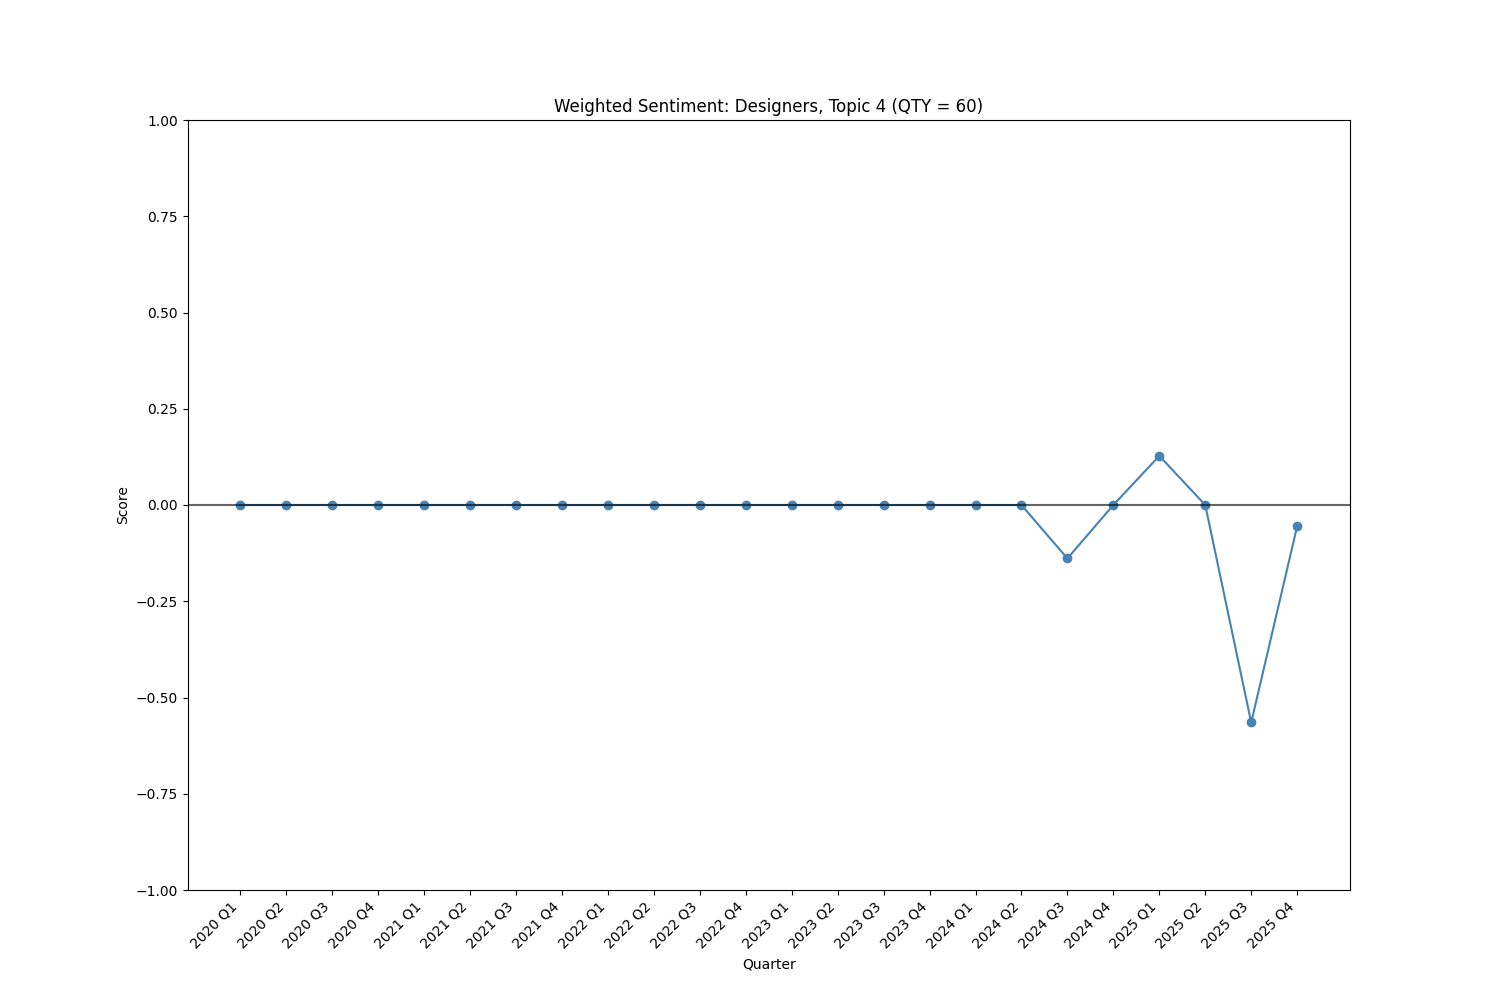
\includegraphics[width=0.80\linewidth]{Images/Appendices/Sentiment/BERTopic/designers_bert_weighted_topic_4.png}
    \caption{Designers topic 4}
\end{figure}
\begin{figure}[H]
    \centering
    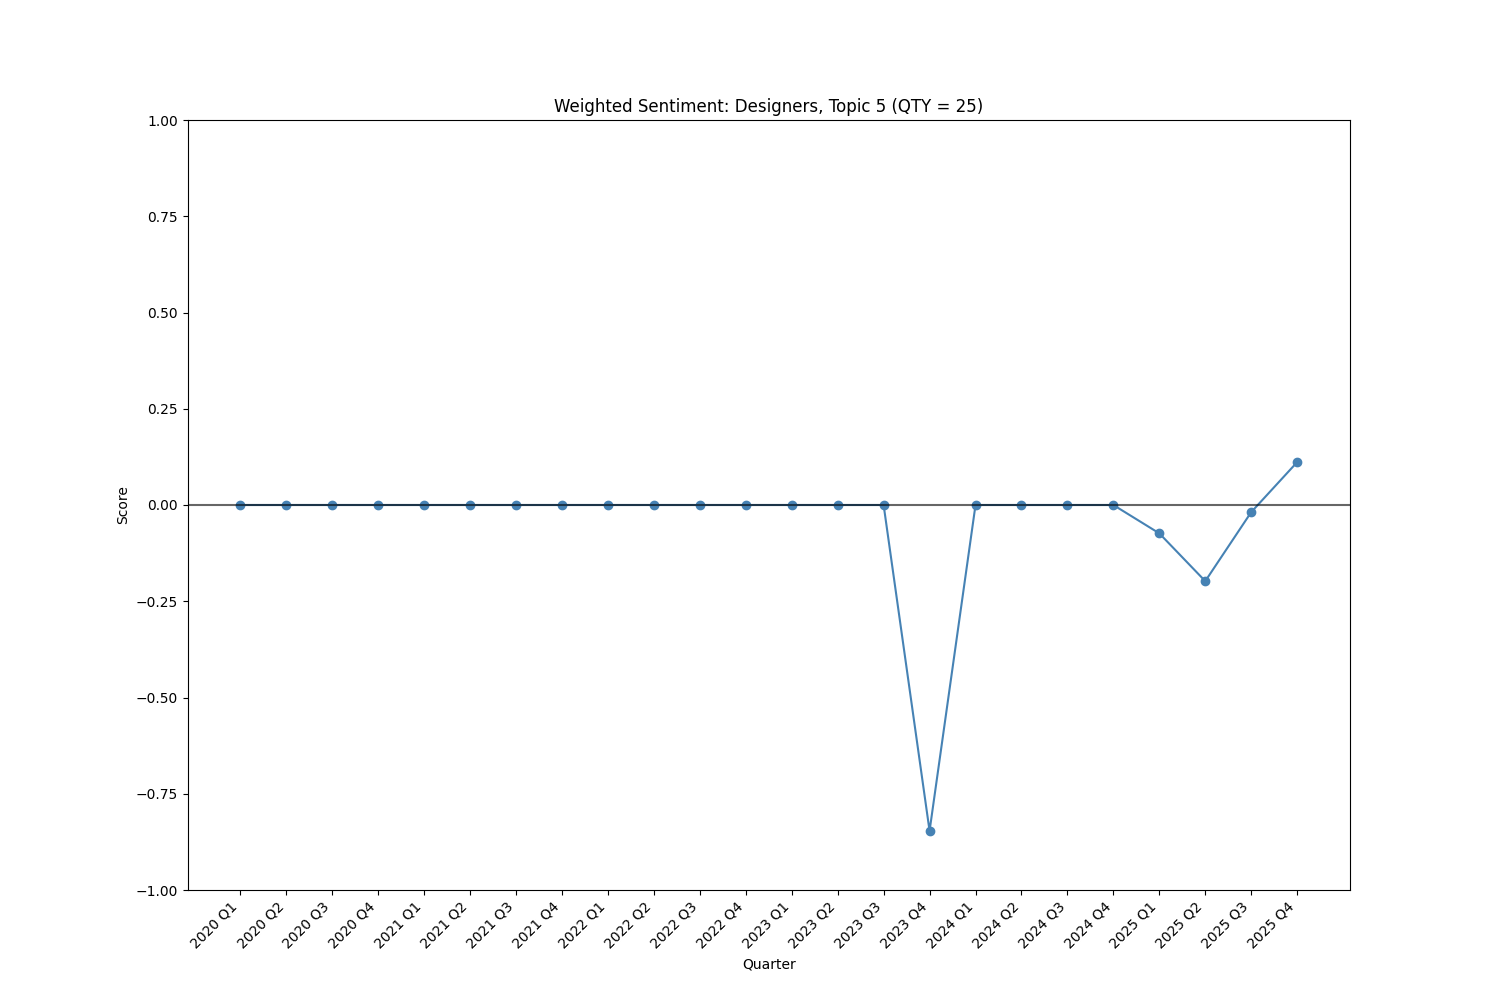
\includegraphics[width=0.80\linewidth]{Images/Appendices/Sentiment/BERTopic/designers_bert_weighted_topic_5.png}
    \caption{Designers topic 5}
\end{figure}
\begin{figure}[H]
    \centering
    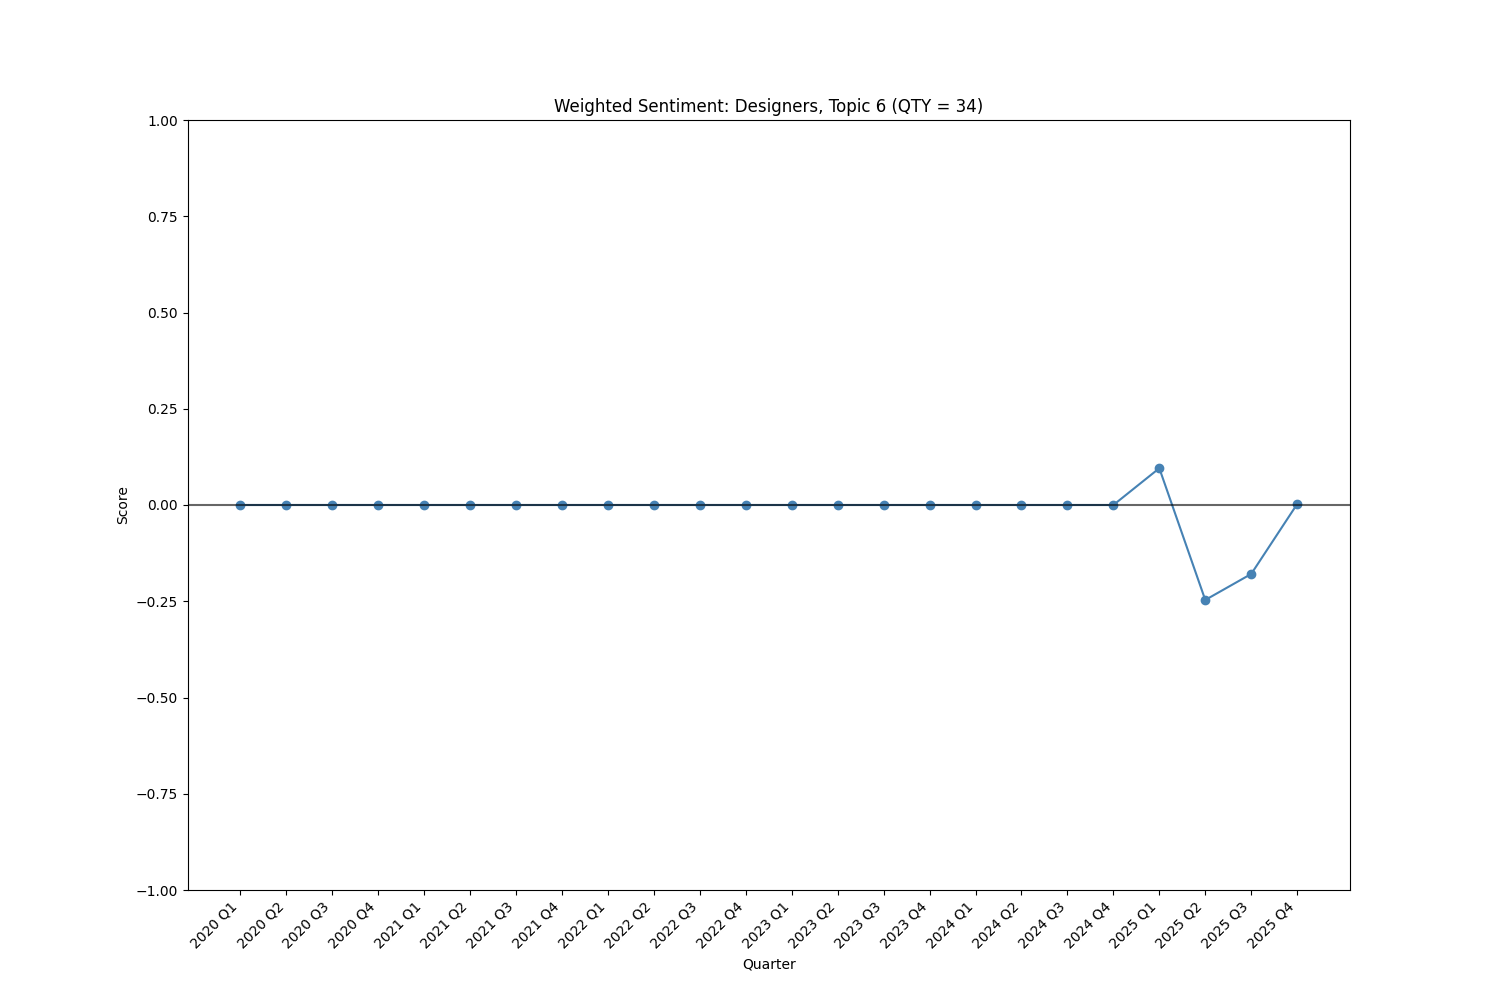
\includegraphics[width=0.80\linewidth]{Images/Appendices/Sentiment/BERTopic/designers_bert_weighted_topic_6.png}
    \caption{Designers topic 6}
\end{figure}

\begin{figure}[H]
    \centering
    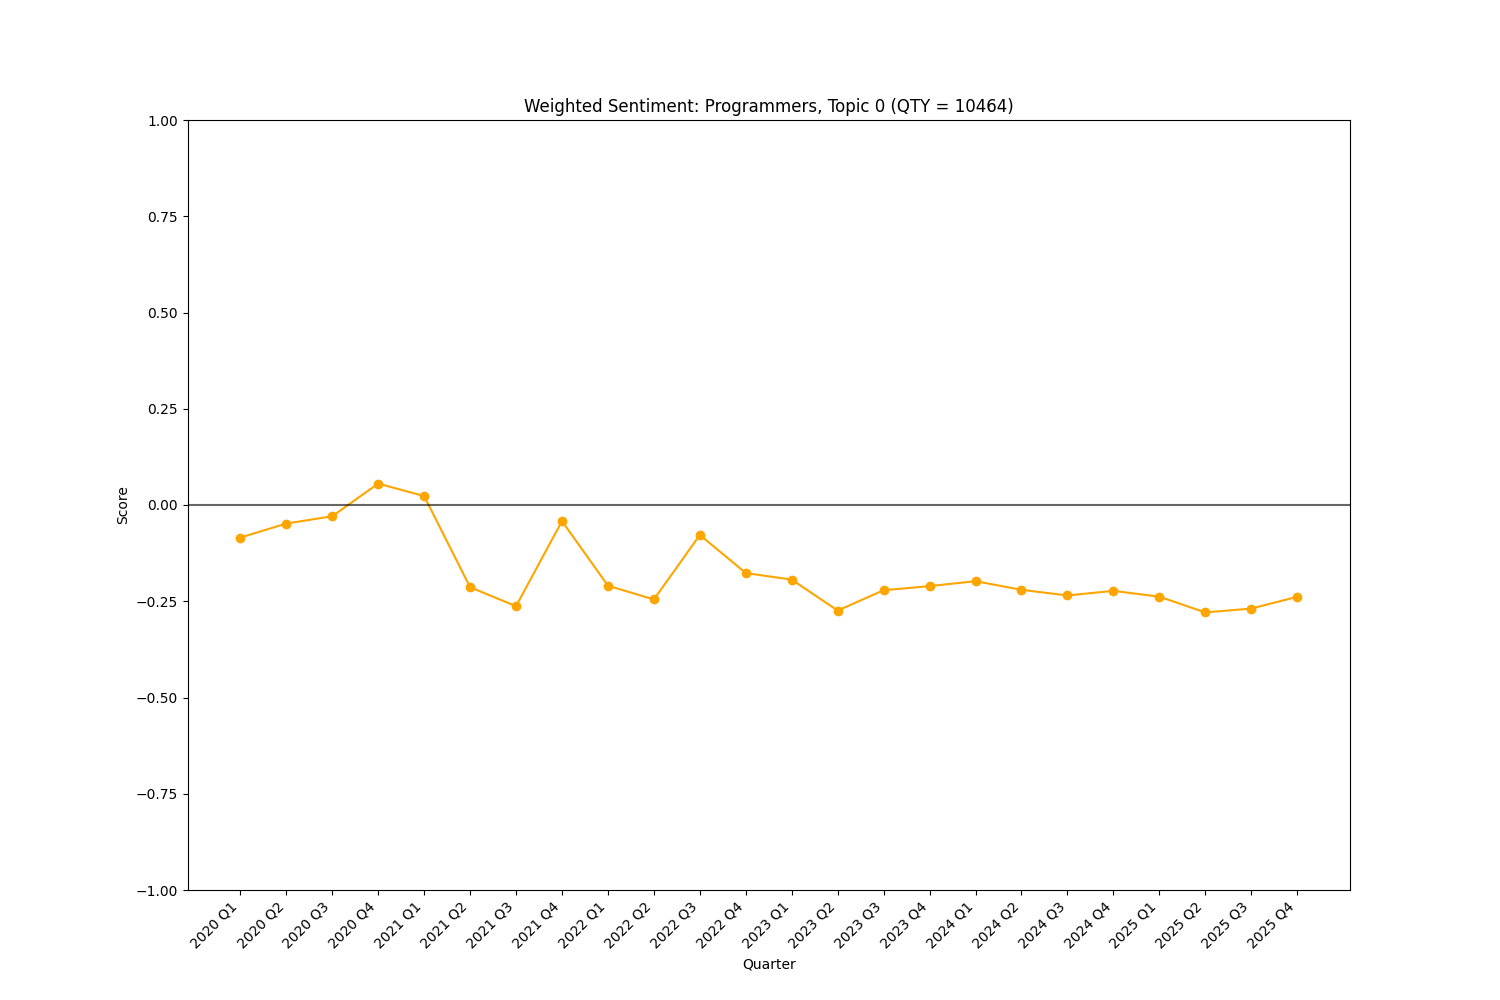
\includegraphics[width=0.80\linewidth]{Images/Appendices/Sentiment/BERTopic/programmers_bert_weighted_topic_0.png}
    \caption{Programmers topic 0}
\end{figure}
\begin{figure}[H]
    \centering
    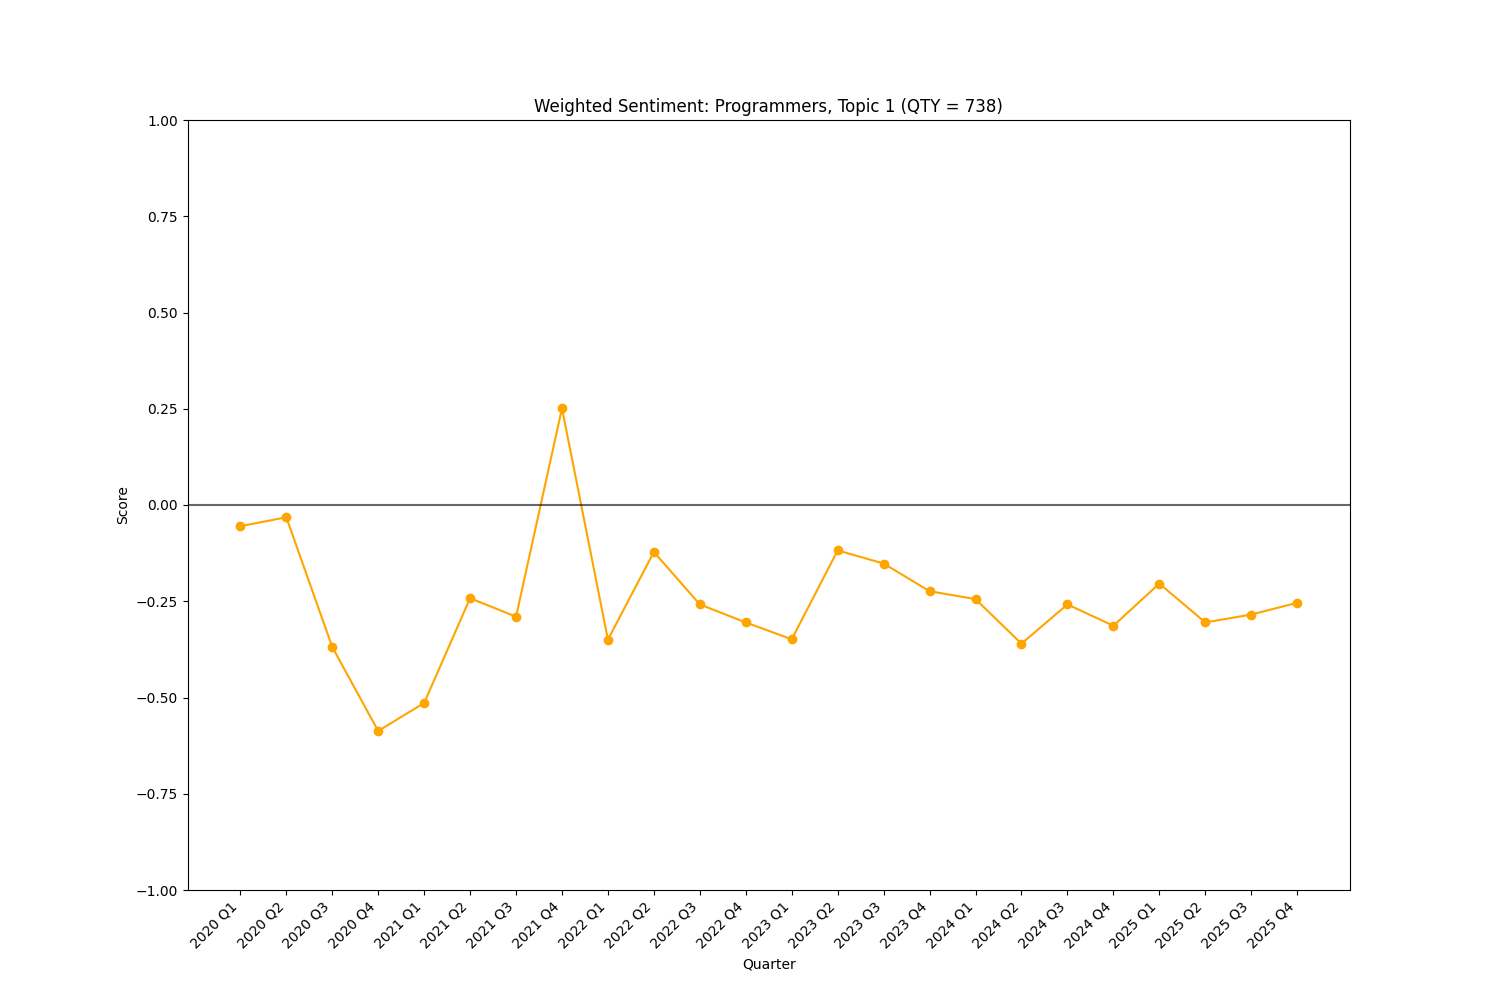
\includegraphics[width=0.80\linewidth]{Images/Appendices/Sentiment/BERTopic/programmers_bert_weighted_topic_1.png}
    \caption{Programmers topic 1}
\end{figure}
\begin{figure}[H]
    \centering
    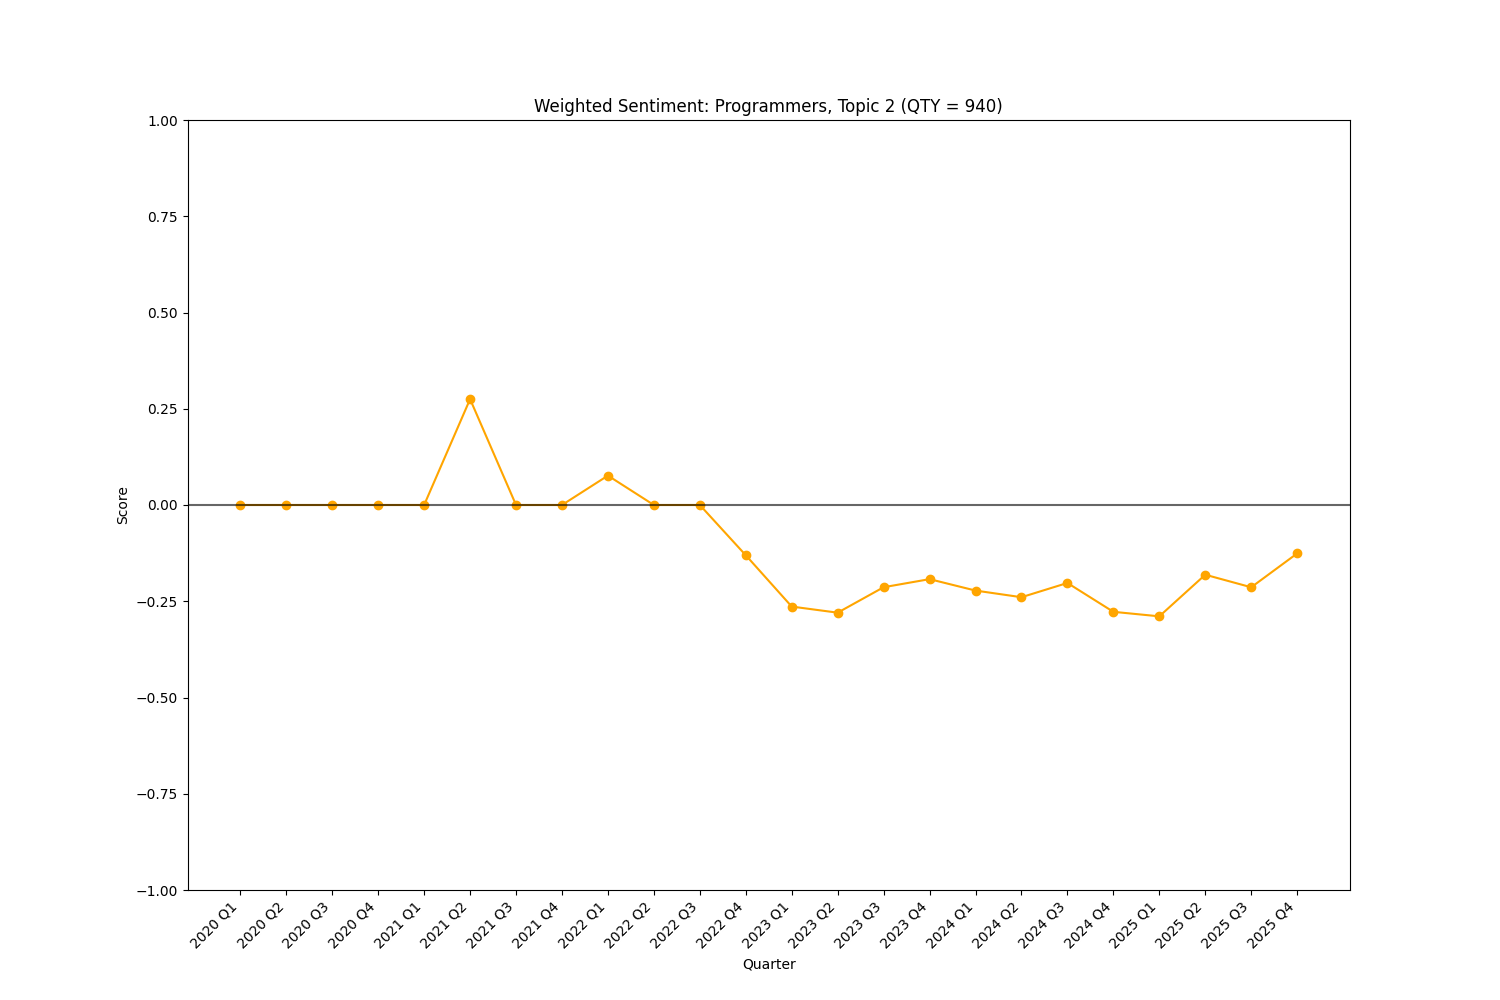
\includegraphics[width=0.80\linewidth]{Images/Appendices/Sentiment/BERTopic/programmers_bert_weighted_topic_2.png}
    \caption{Programmers topic 2}
\end{figure}
\begin{figure}[H]
    \centering
    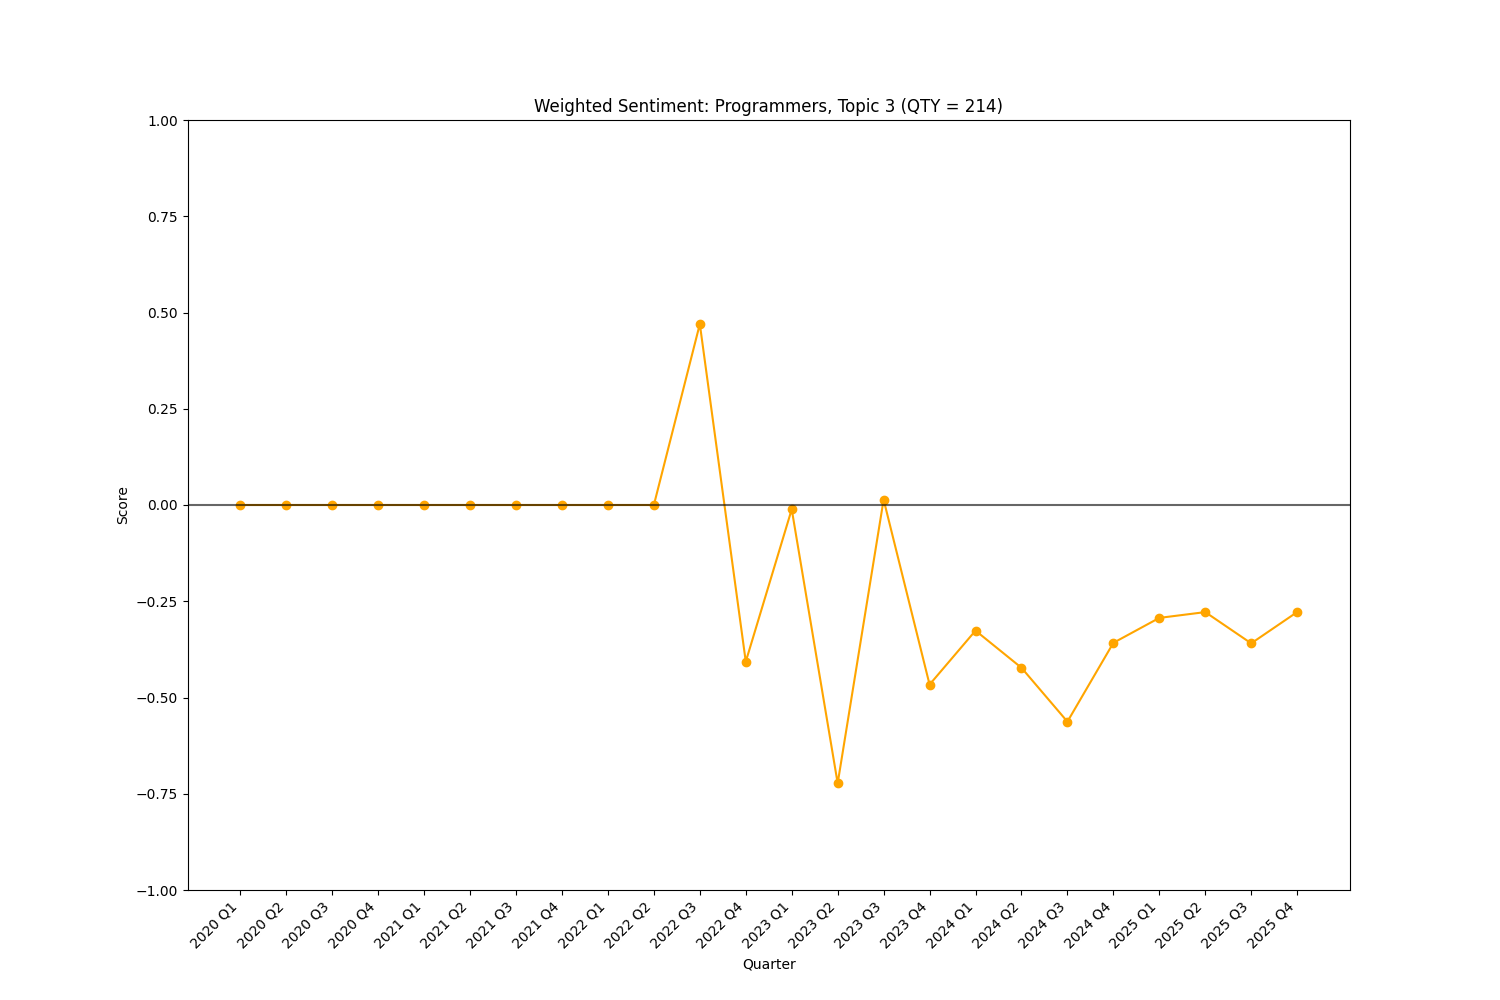
\includegraphics[width=0.80\linewidth]{Images/Appendices/Sentiment/BERTopic/programmers_bert_weighted_topic_3.png}
    \caption{Programmers topic 3}
\end{figure}
\begin{figure}[H]
    \centering
    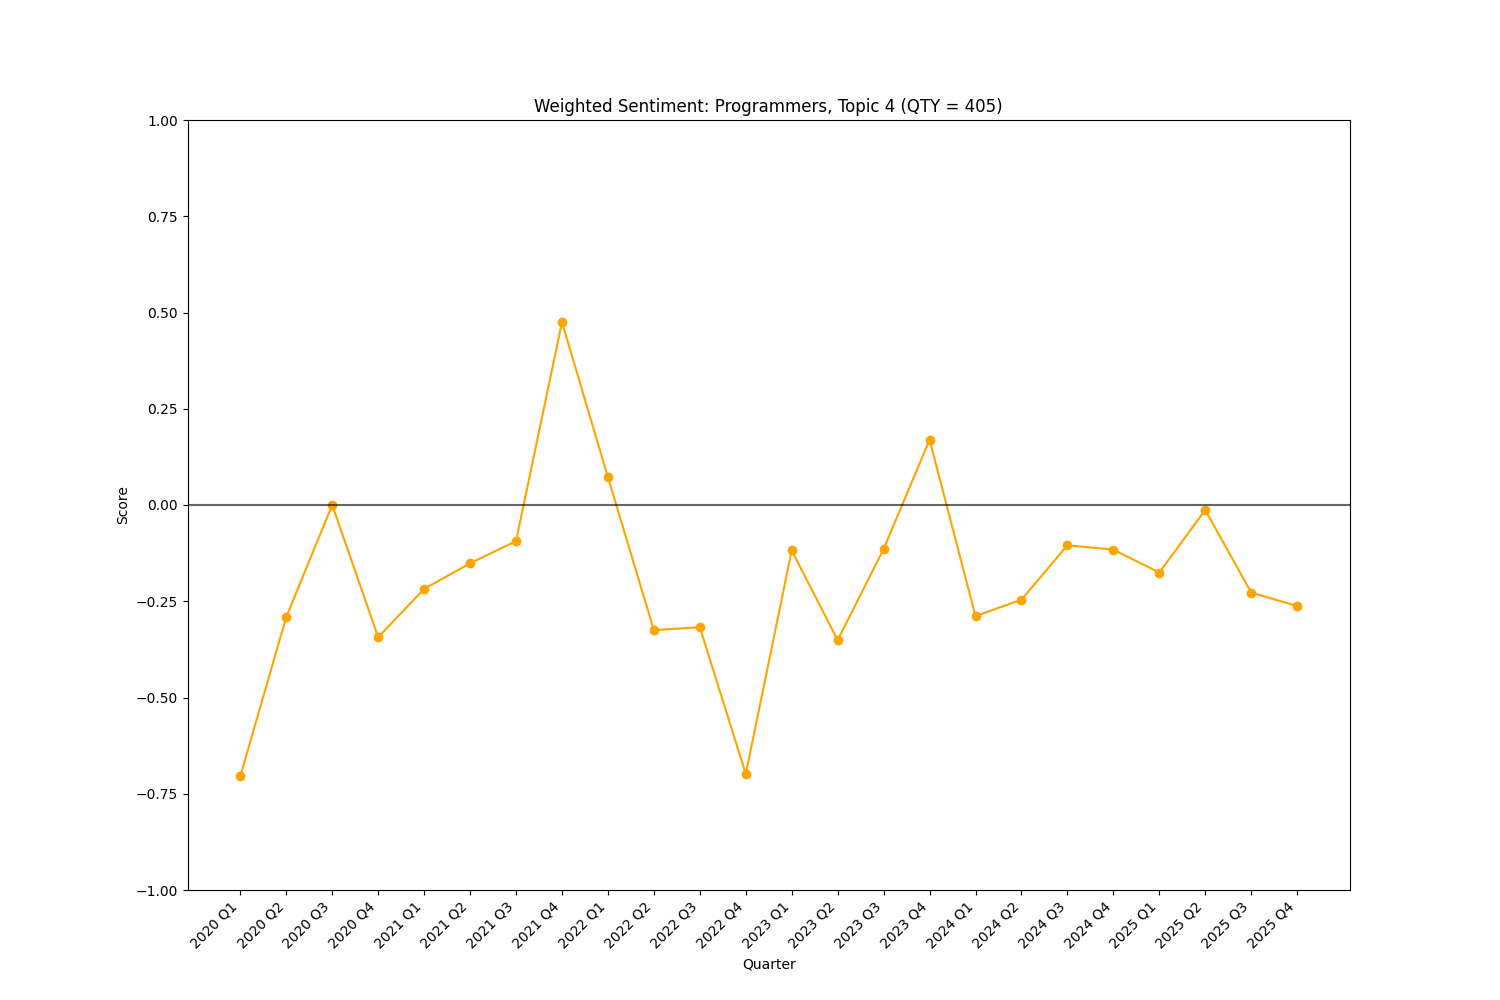
\includegraphics[width=0.80\linewidth]{Images/Appendices/Sentiment/BERTopic/programmers_bert_weighted_topic_4.png}
    \caption{Programmers topic 4}
\end{figure}
\begin{figure}[H]
    \centering
    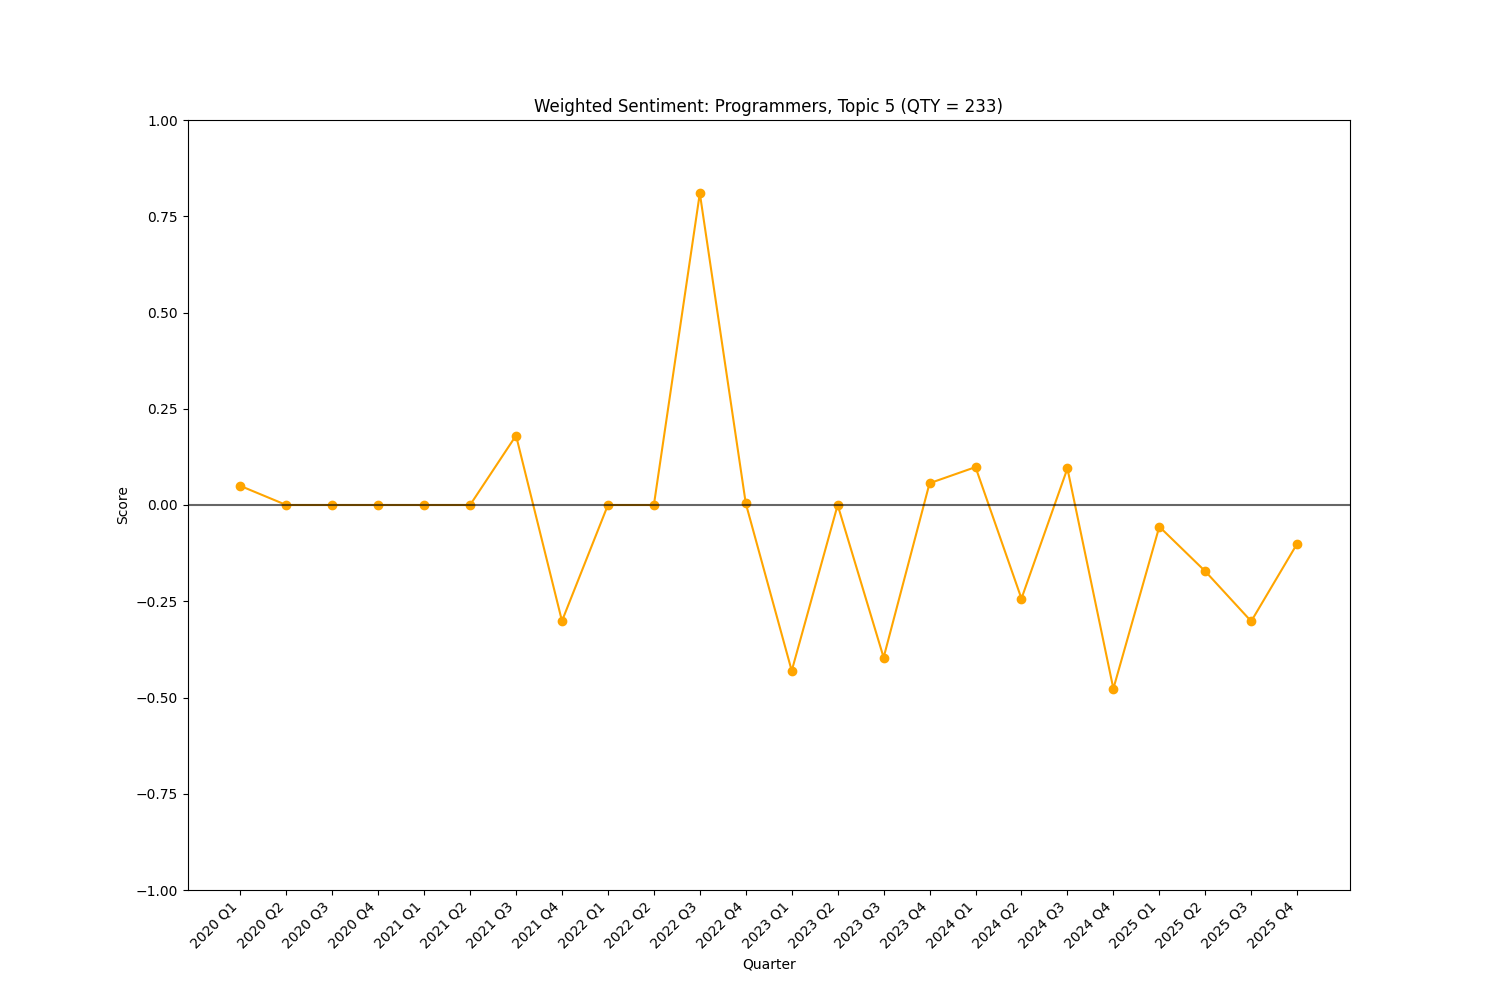
\includegraphics[width=0.80\linewidth]{Images/Appendices/Sentiment/BERTopic/programmers_bert_weighted_topic_5.png}
    \caption{Programmers topic 5}
\end{figure}
\begin{figure}[H]
    \centering
    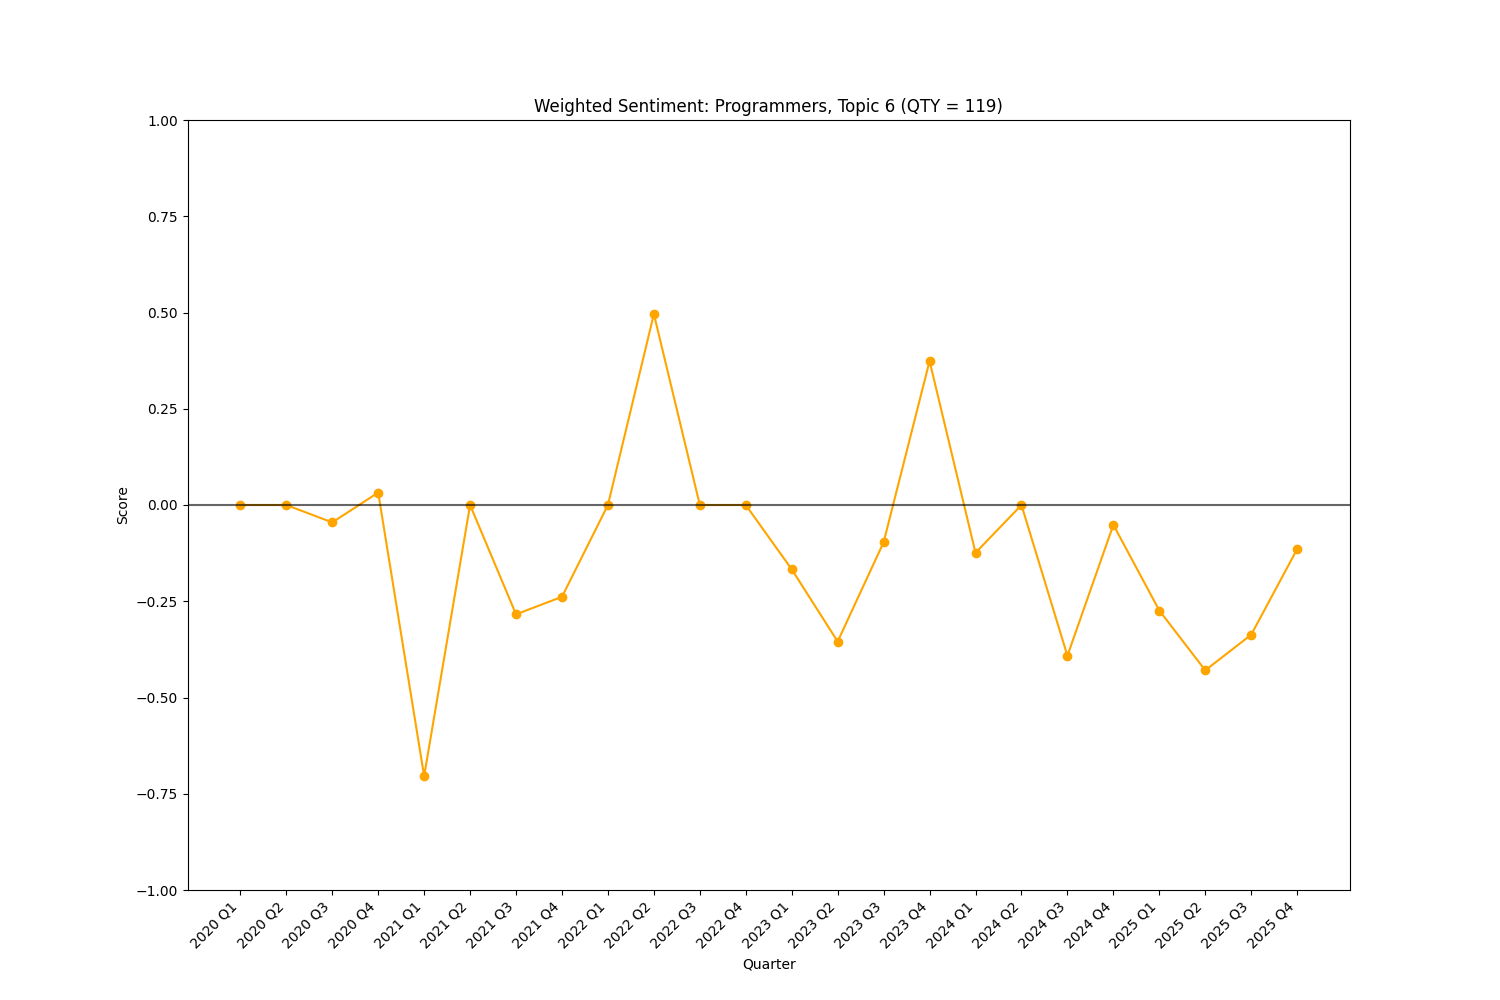
\includegraphics[width=0.80\linewidth]{Images/Appendices/Sentiment/BERTopic/programmers_bert_weighted_topic_6.png}
    \caption{Programmers topic 6}
\end{figure}
\begin{figure}[H]
    \centering
    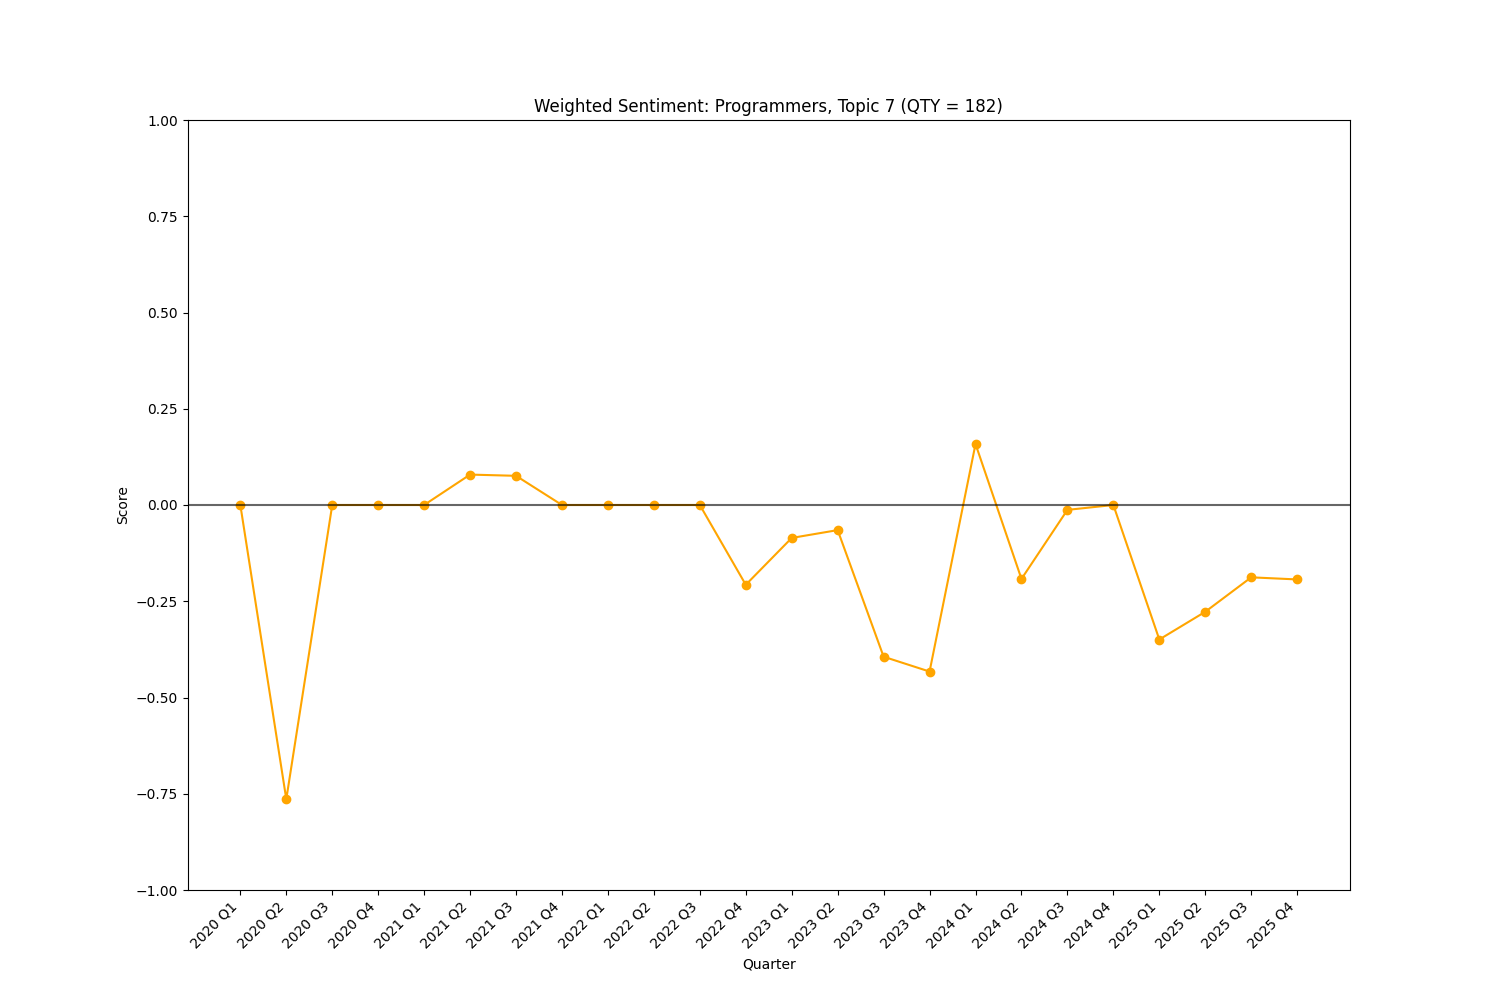
\includegraphics[width=0.80\linewidth]{Images/Appendices/Sentiment/BERTopic/programmers_bert_weighted_topic_7.png}
    \caption{Programmers topic 7}
\end{figure}
\begin{figure}[H]
    \centering
    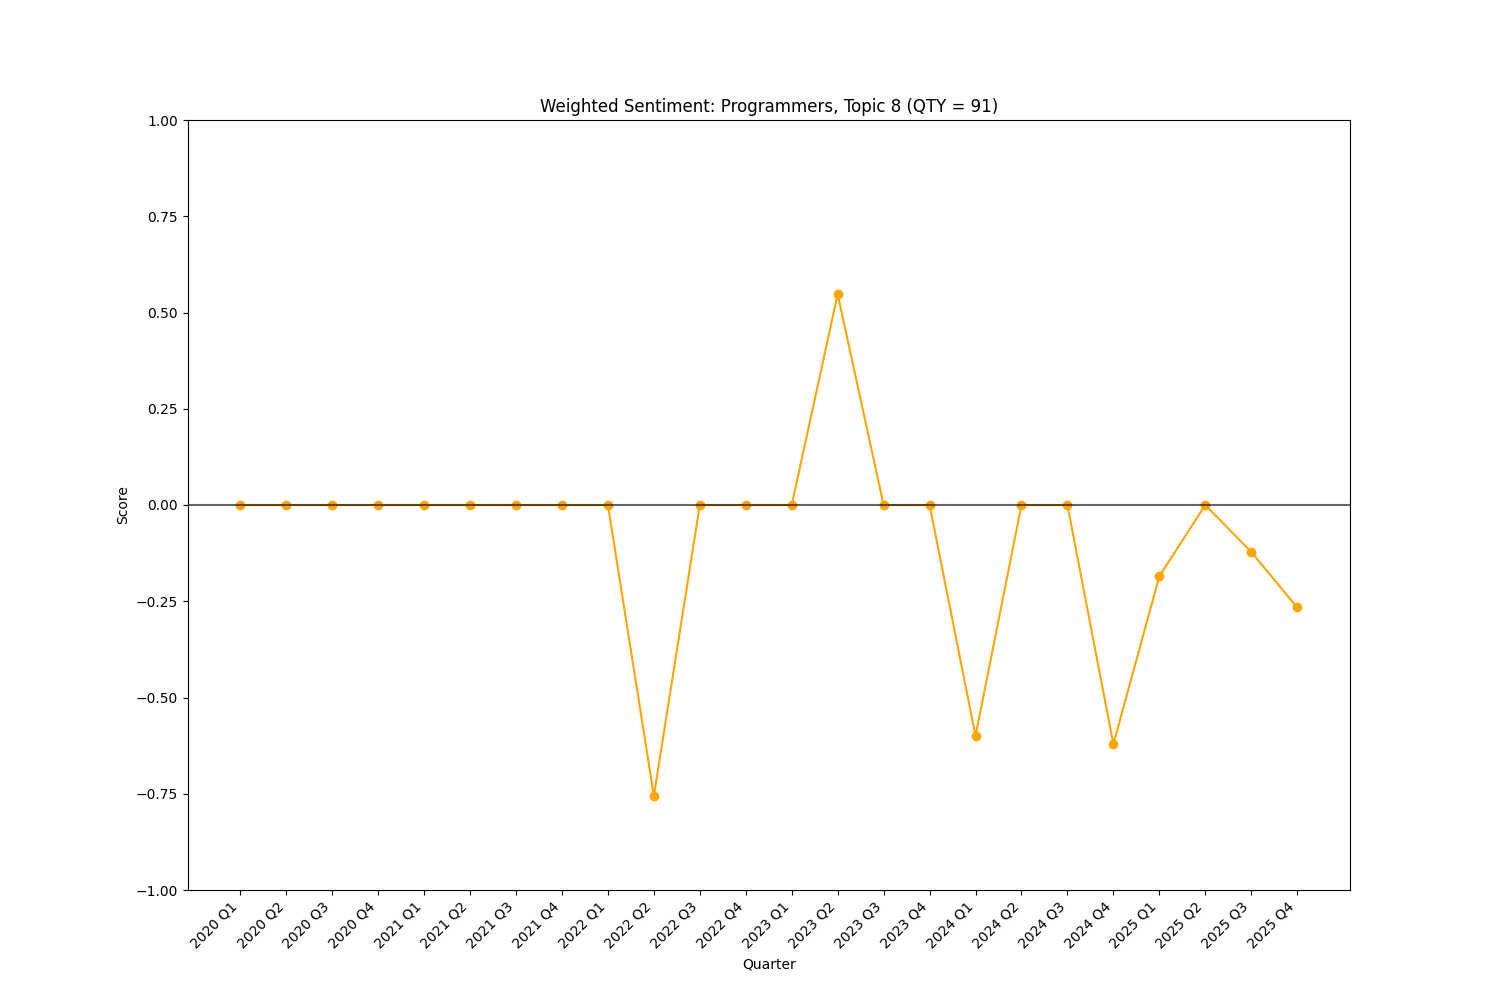
\includegraphics[width=0.80\linewidth]{Images/Appendices/Sentiment/BERTopic/programmers_bert_weighted_topic_8.png}
    \caption{Programmers topic 8}
\end{figure}
\begin{figure}[H]
    \centering
    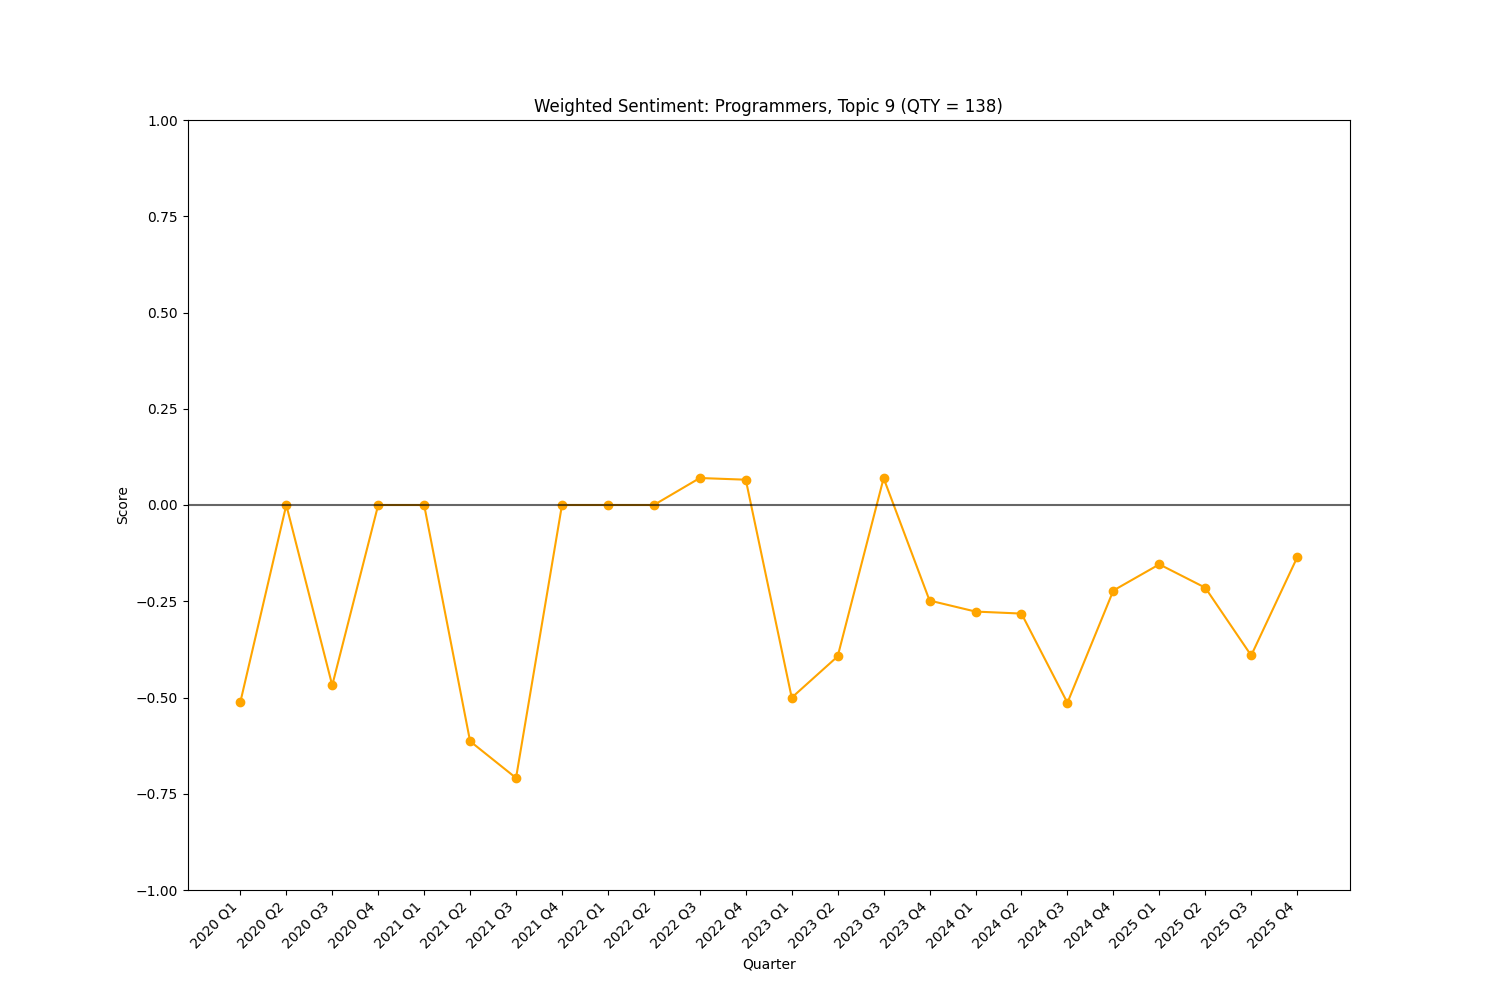
\includegraphics[width=0.80\linewidth]{Images/Appendices/Sentiment/BERTopic/programmers_bert_weighted_topic_9.png}
    \caption{Programmers topic 9}
\end{figure}

\subsection{Louvain}
\begin{figure}[H]
    \centering
    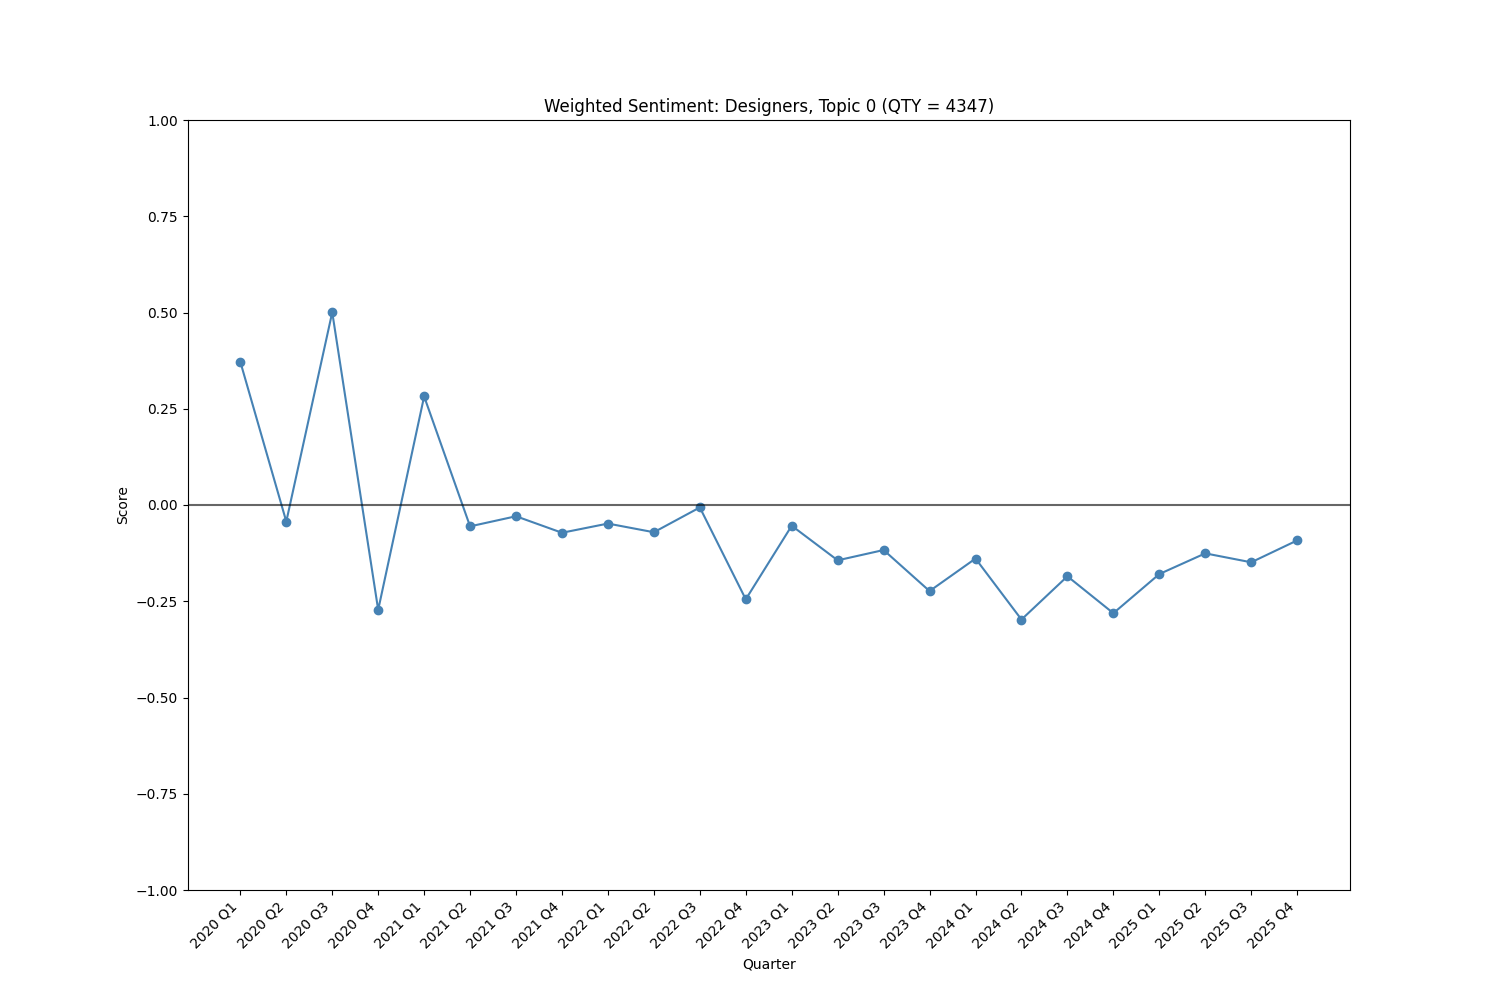
\includegraphics[width=0.80\linewidth]{Images/Appendices/Sentiment/Louvain/designers_louvain_weighted_topic_0.png}
    \caption{Designers topic 0}
\end{figure}
\begin{figure}[H]
    \centering
    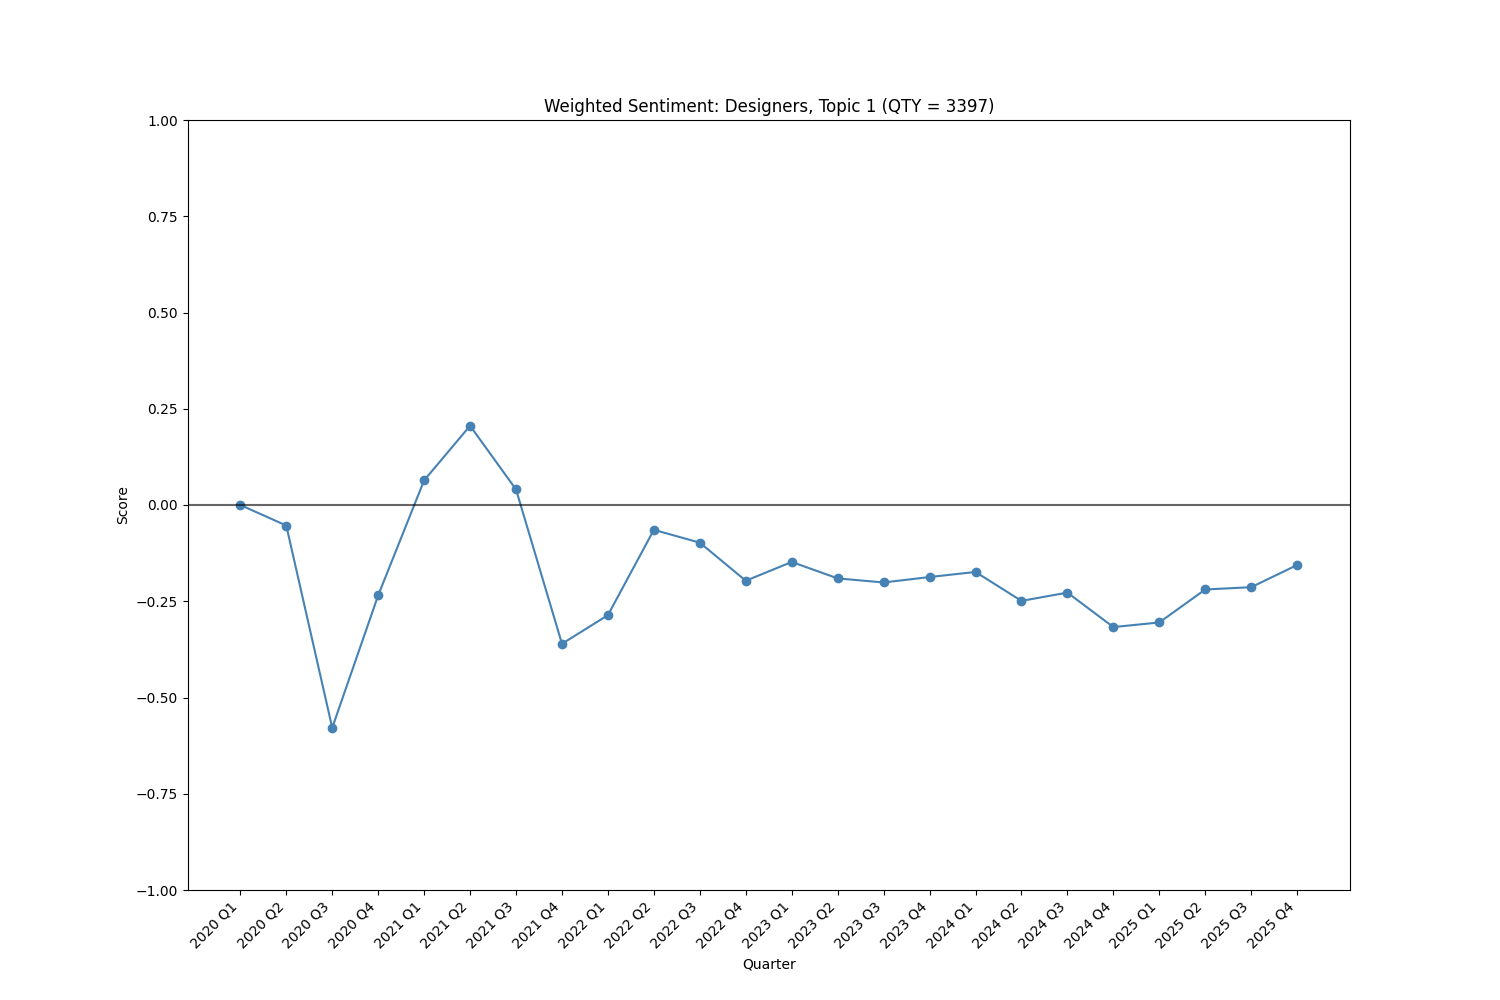
\includegraphics[width=0.80\linewidth]{Images/Appendices/Sentiment/Louvain/designers_louvain_weighted_topic_1.png}
    \caption{Designers topic 1}
\end{figure}
\begin{figure}[H]
    \centering
    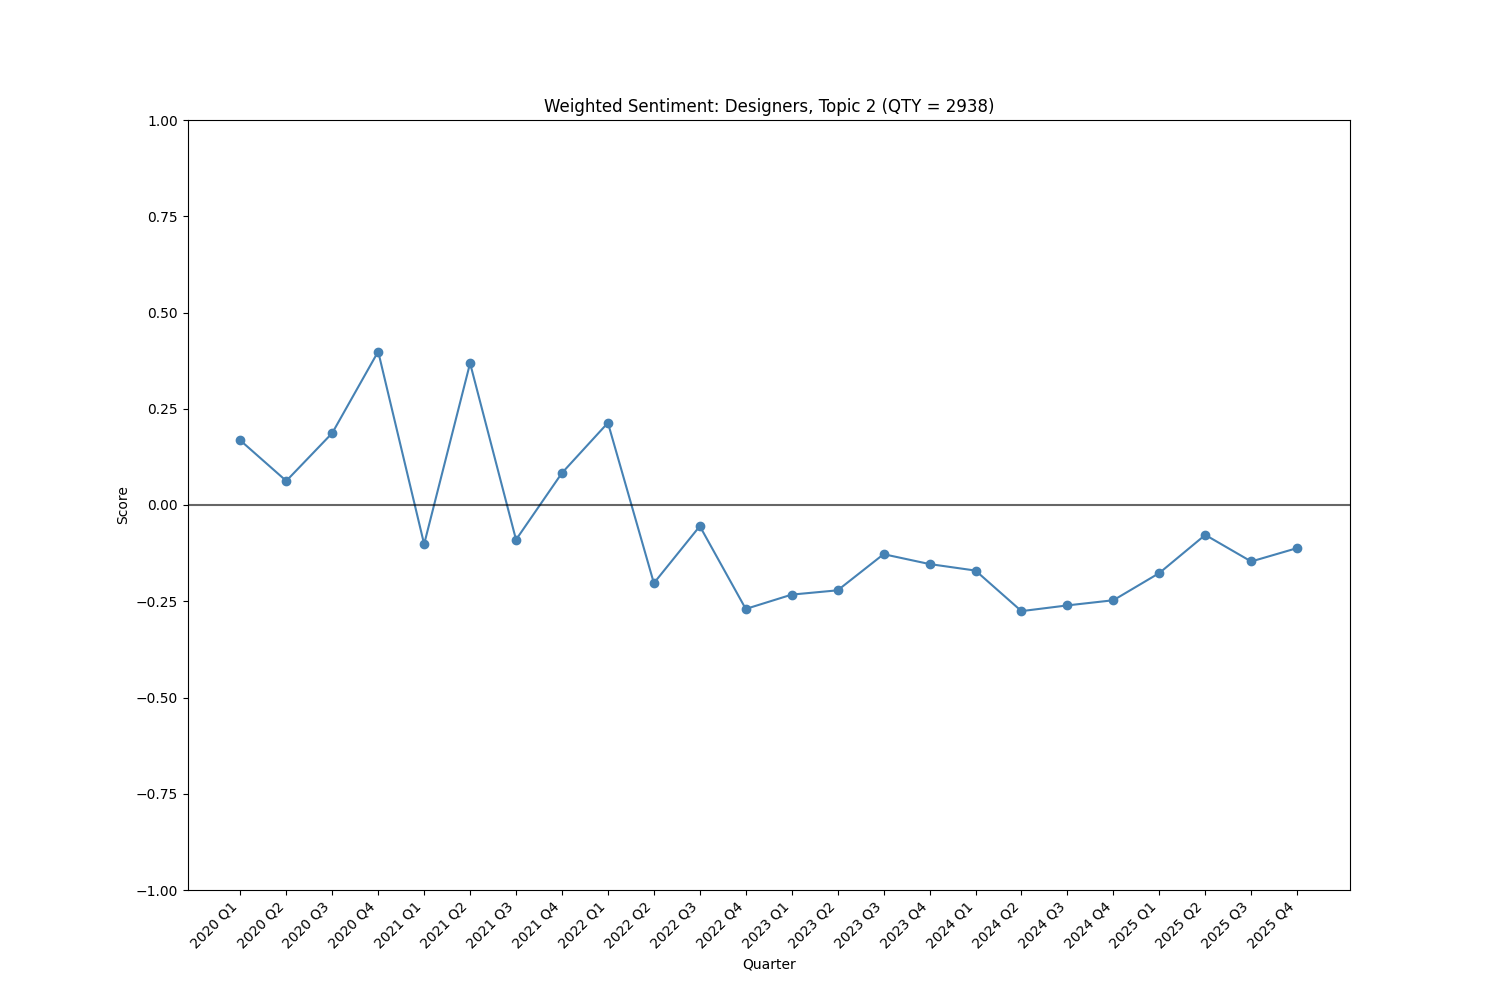
\includegraphics[width=0.80\linewidth]{Images/Appendices/Sentiment/Louvain/designers_louvain_weighted_topic_2.png}
    \caption{Designers topic 2}
\end{figure}
\begin{figure}[H]
    \centering
    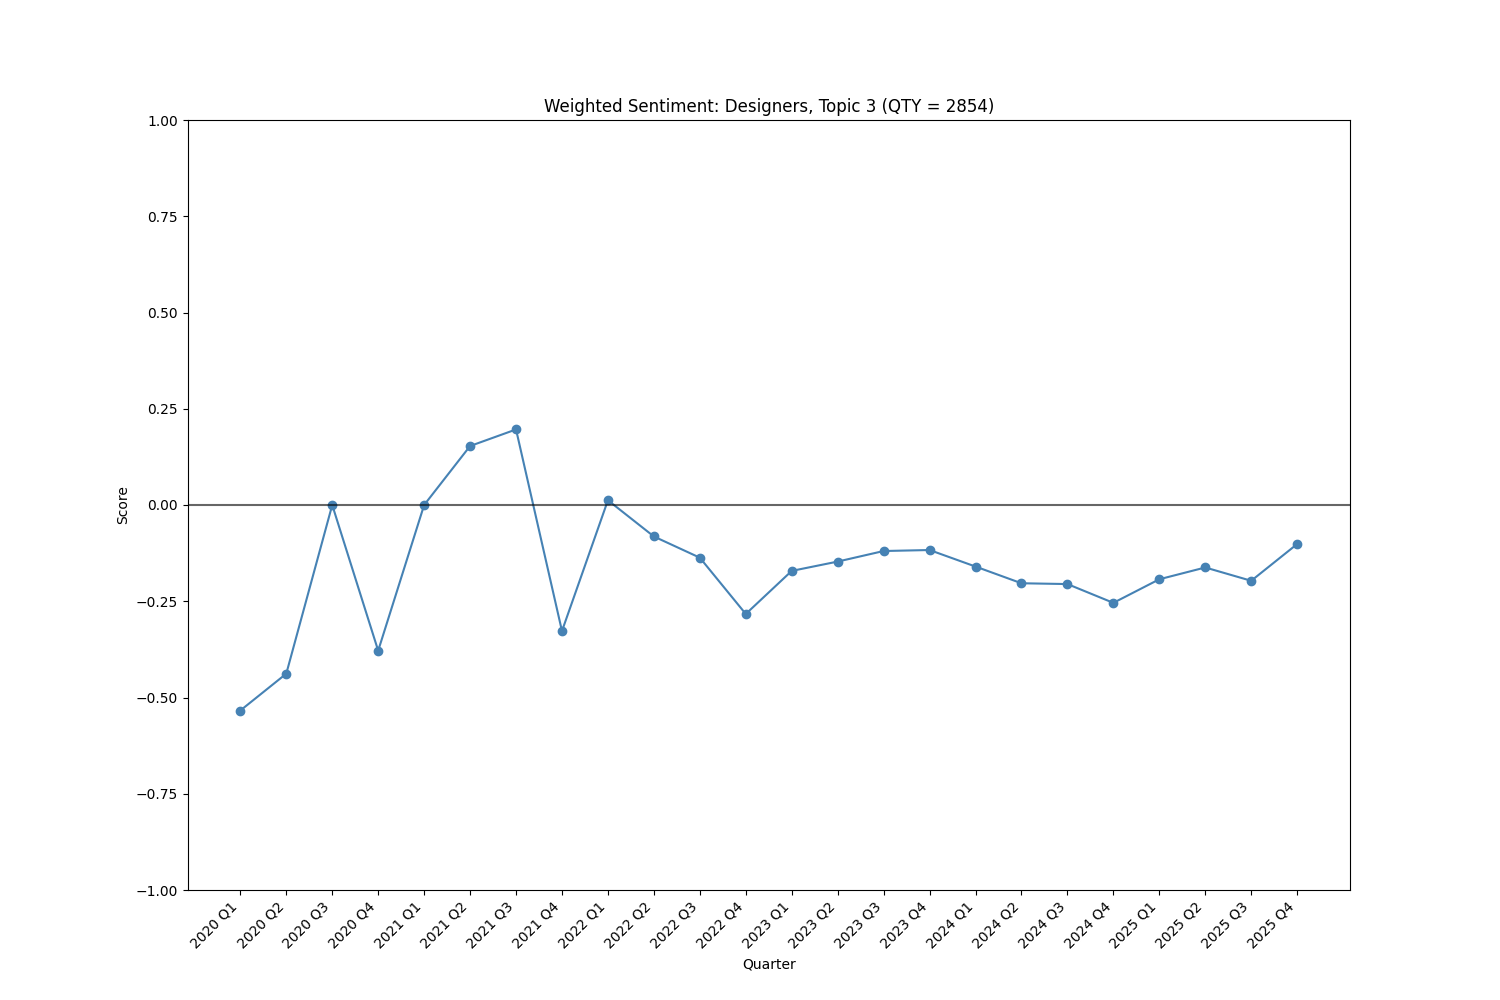
\includegraphics[width=0.80\linewidth]{Images/Appendices/Sentiment/Louvain/designers_louvain_weighted_topic_3.png}
    \caption{Designers topic 3}
\end{figure}
\begin{figure}[H]
    \centering
    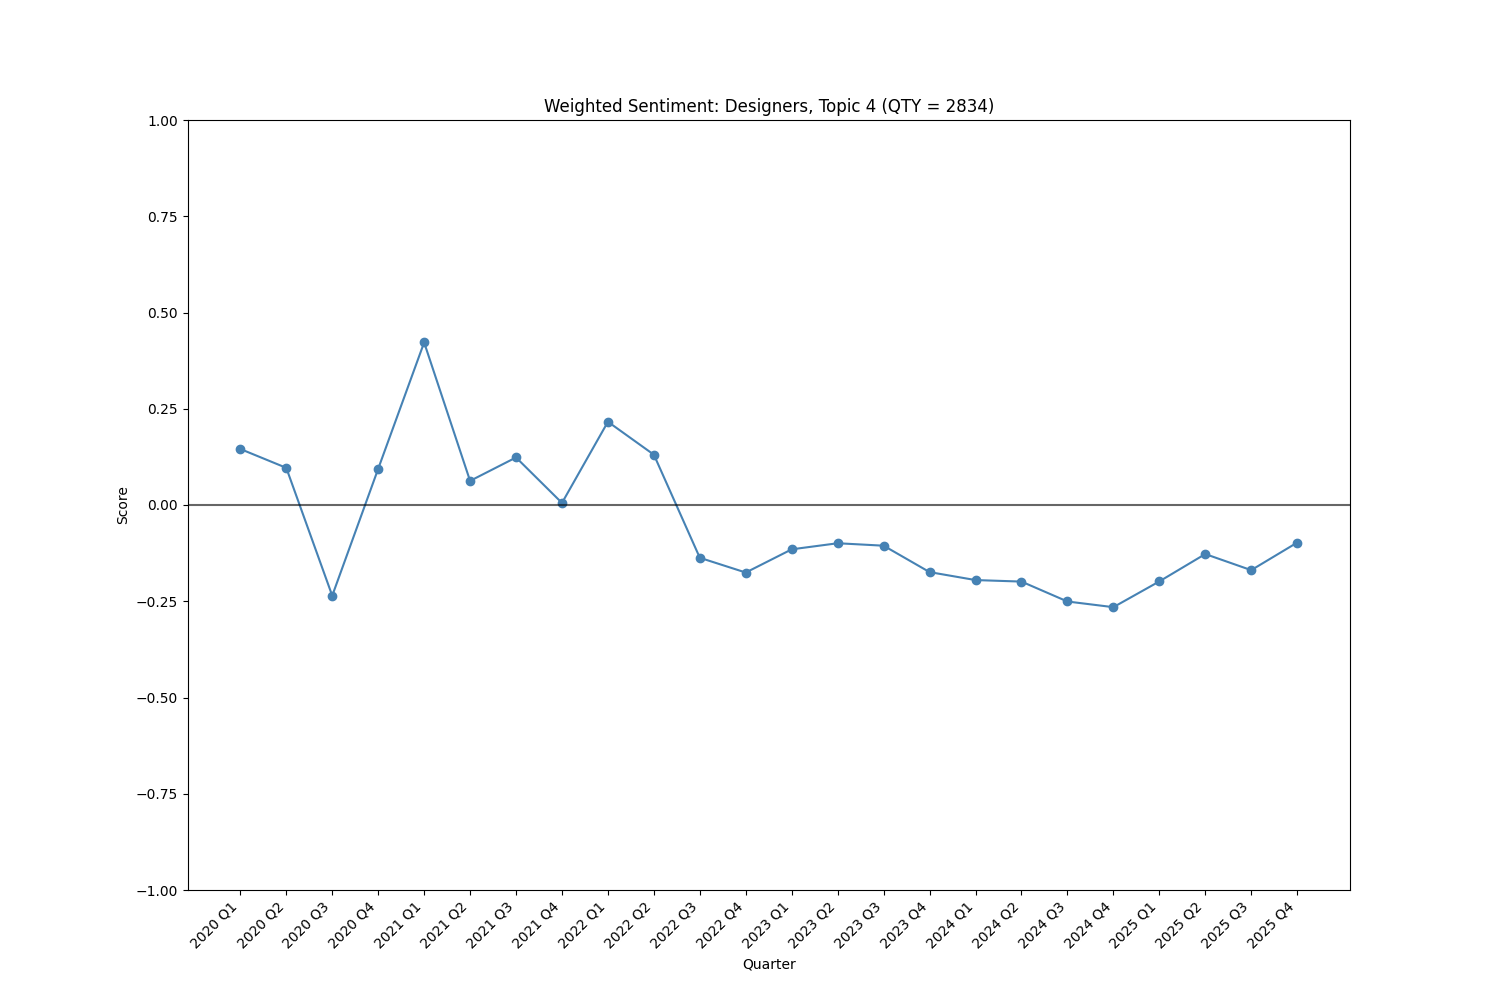
\includegraphics[width=0.80\linewidth]{Images/Appendices/Sentiment/Louvain/designers_louvain_weighted_topic_4.png}
    \caption{Designers topic 4}
\end{figure}
\begin{figure}[H]
    \centering
    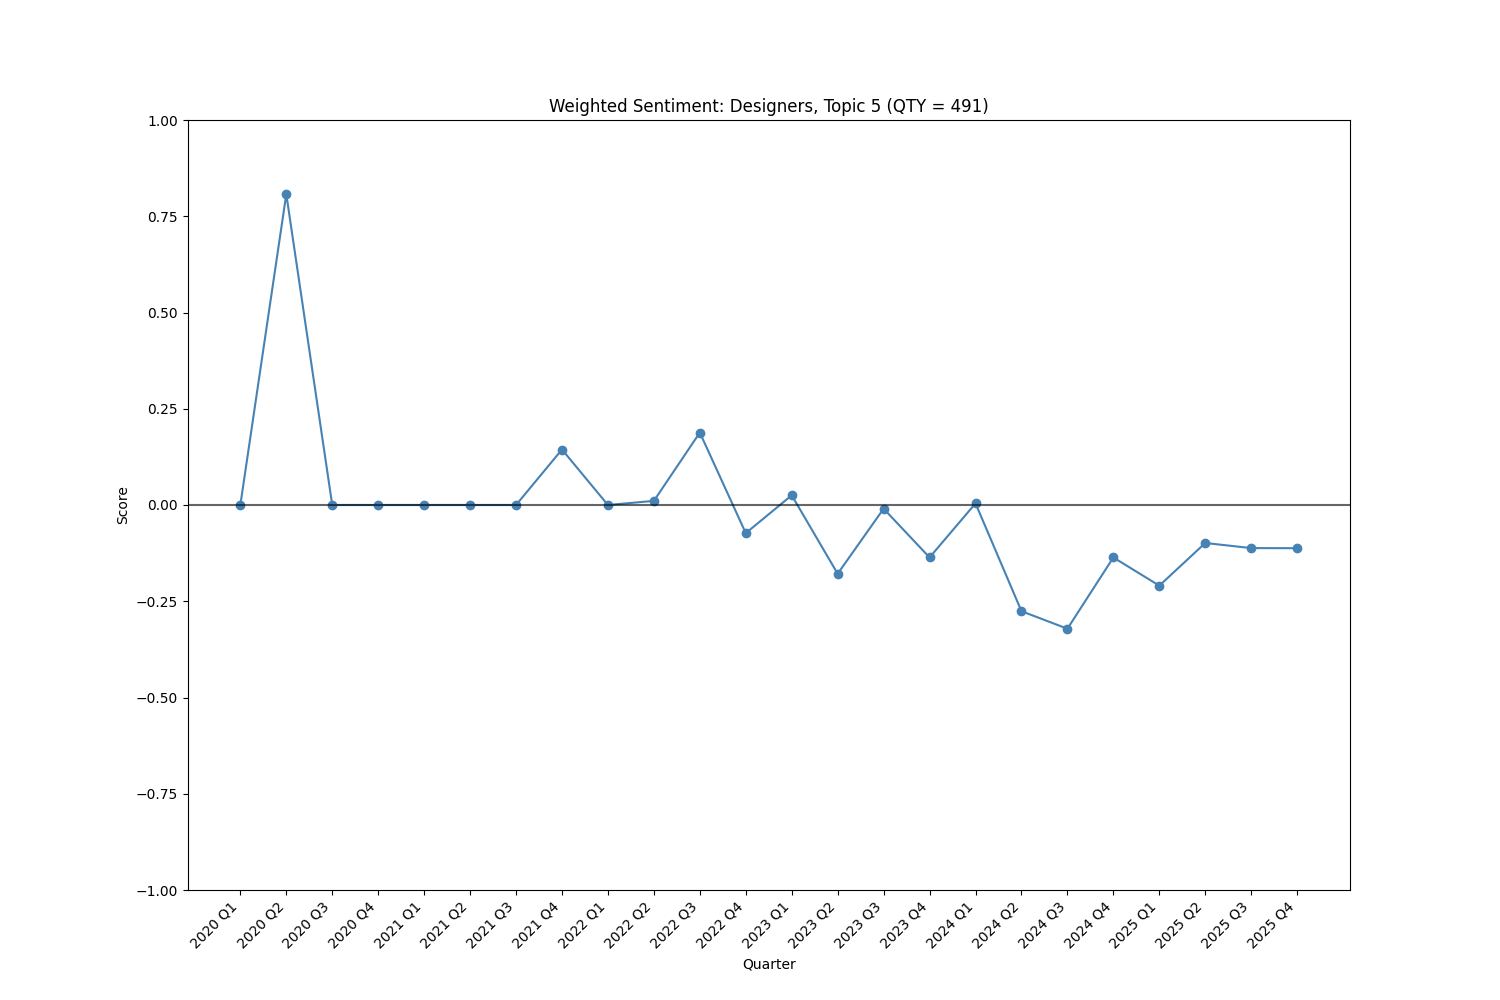
\includegraphics[width=0.80\linewidth]{Images/Appendices/Sentiment/Louvain/designers_louvain_weighted_topic_5.png}
    \caption{Designers topic 5}
\end{figure}
\begin{figure}[H]
    \centering
    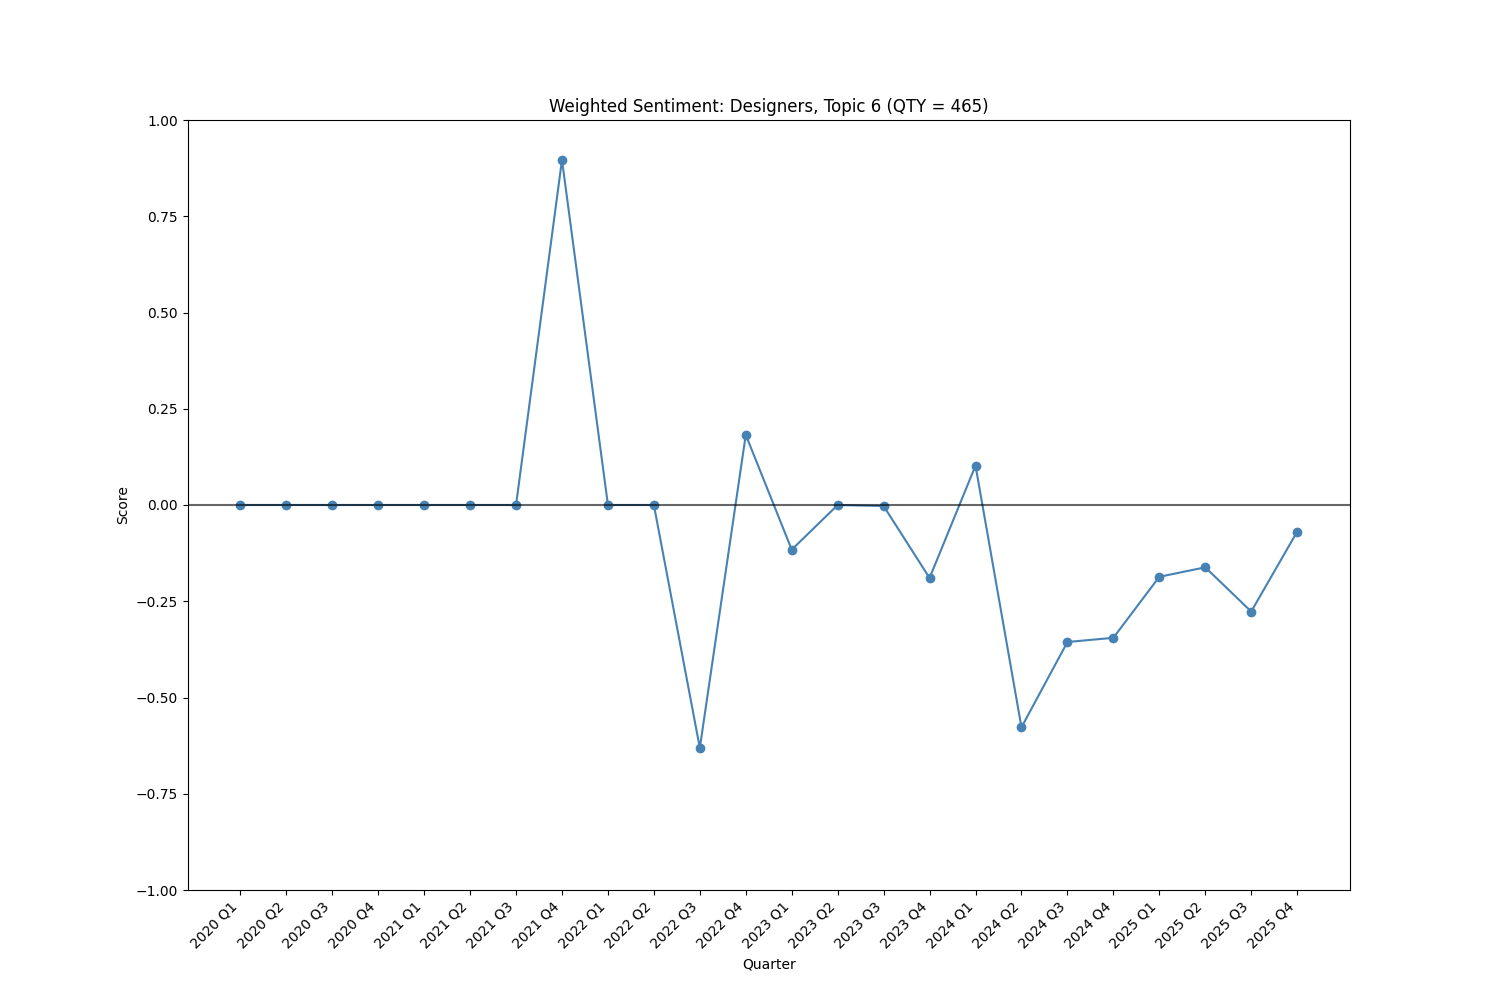
\includegraphics[width=0.80\linewidth]{Images/Appendices/Sentiment/Louvain/designers_louvain_weighted_topic_6.png}
    \caption{Designers topic 6}
\end{figure}
\begin{figure}[H]
    \centering
    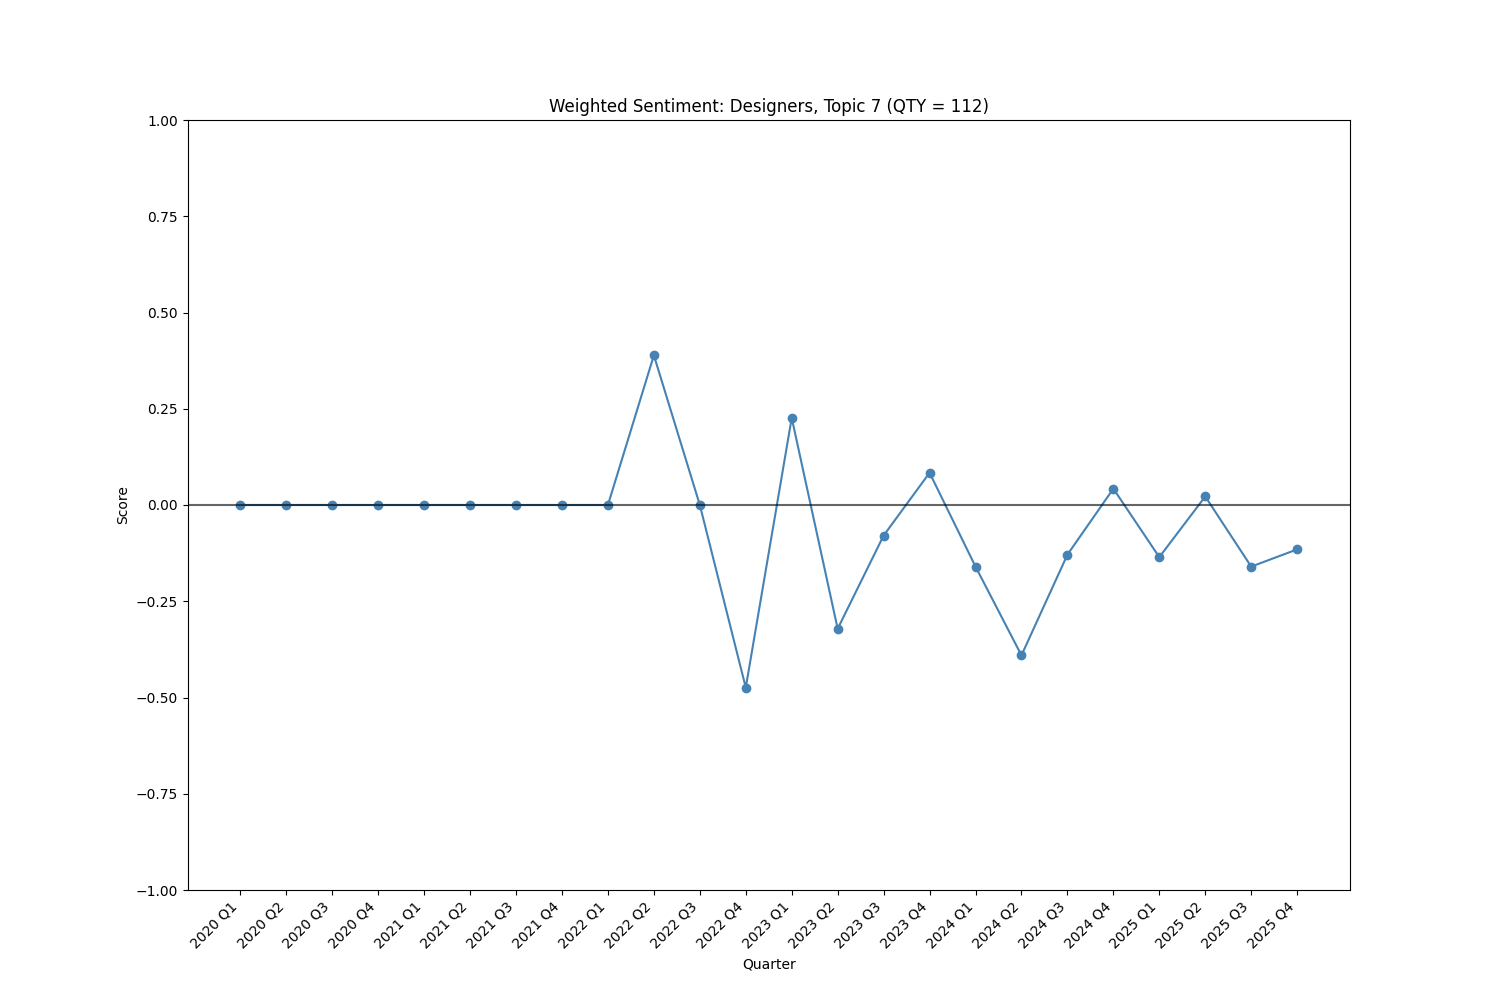
\includegraphics[width=0.80\linewidth]{Images/Appendices/Sentiment/Louvain/designers_louvain_weighted_topic_7.png}
    \caption{Designers topic 7}
\end{figure}

\begin{figure}[H]
    \centering
    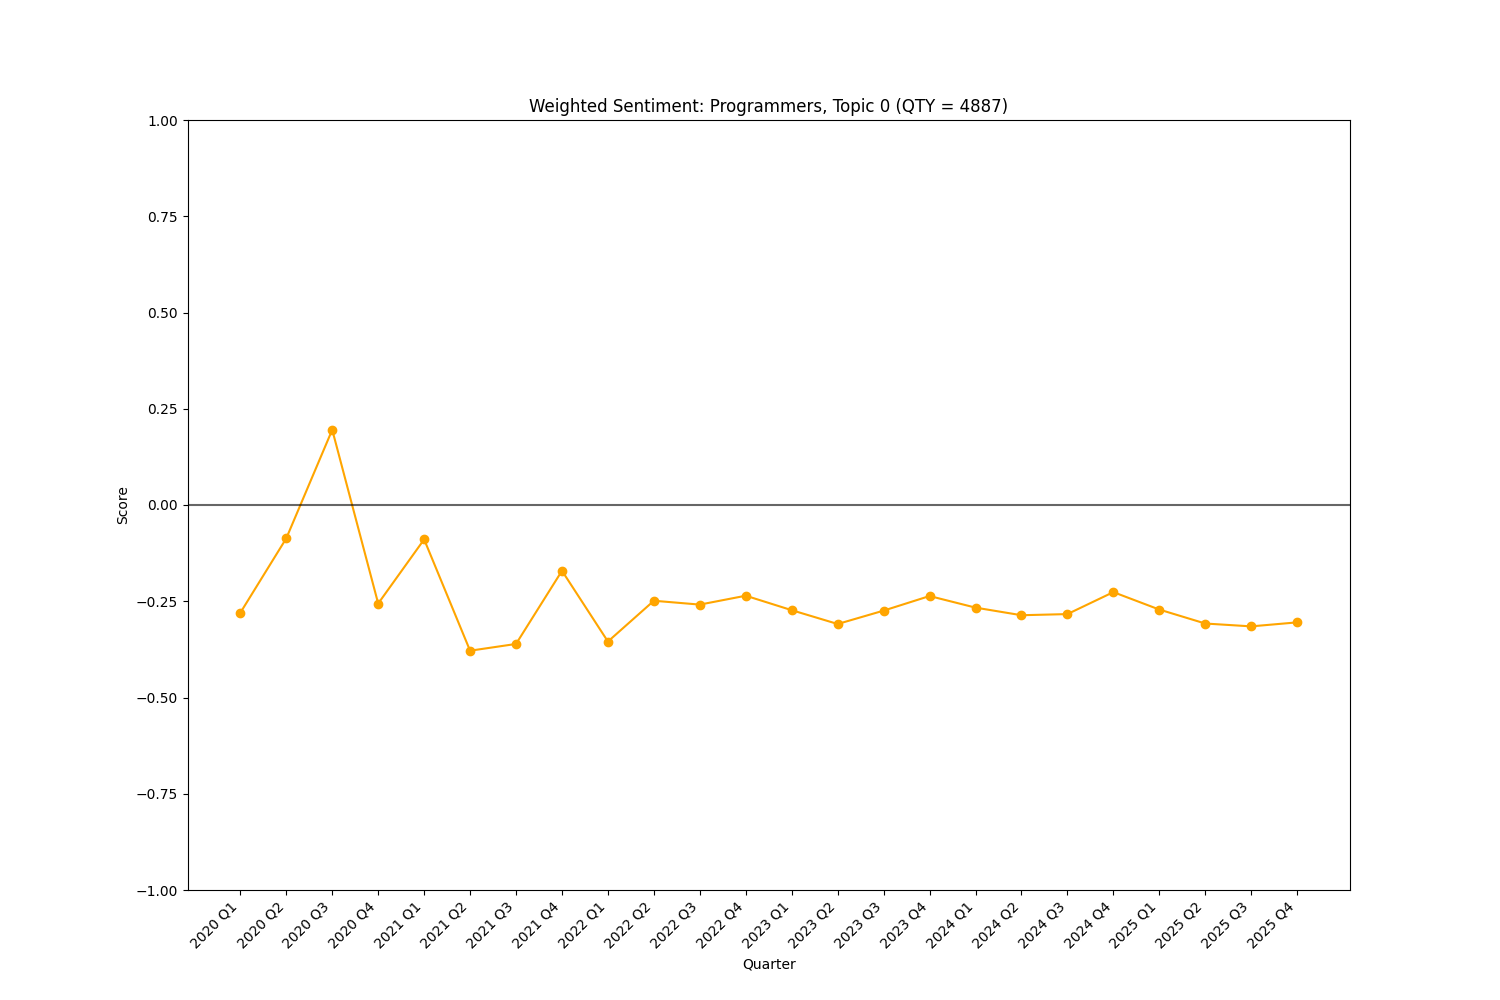
\includegraphics[width=0.80\linewidth]{Images/Appendices/Sentiment/Louvain/programmers_louvain_weighted_topic_0.png}
    \caption{Programmers topic 0}
\end{figure}
\begin{figure}[H]
    \centering
    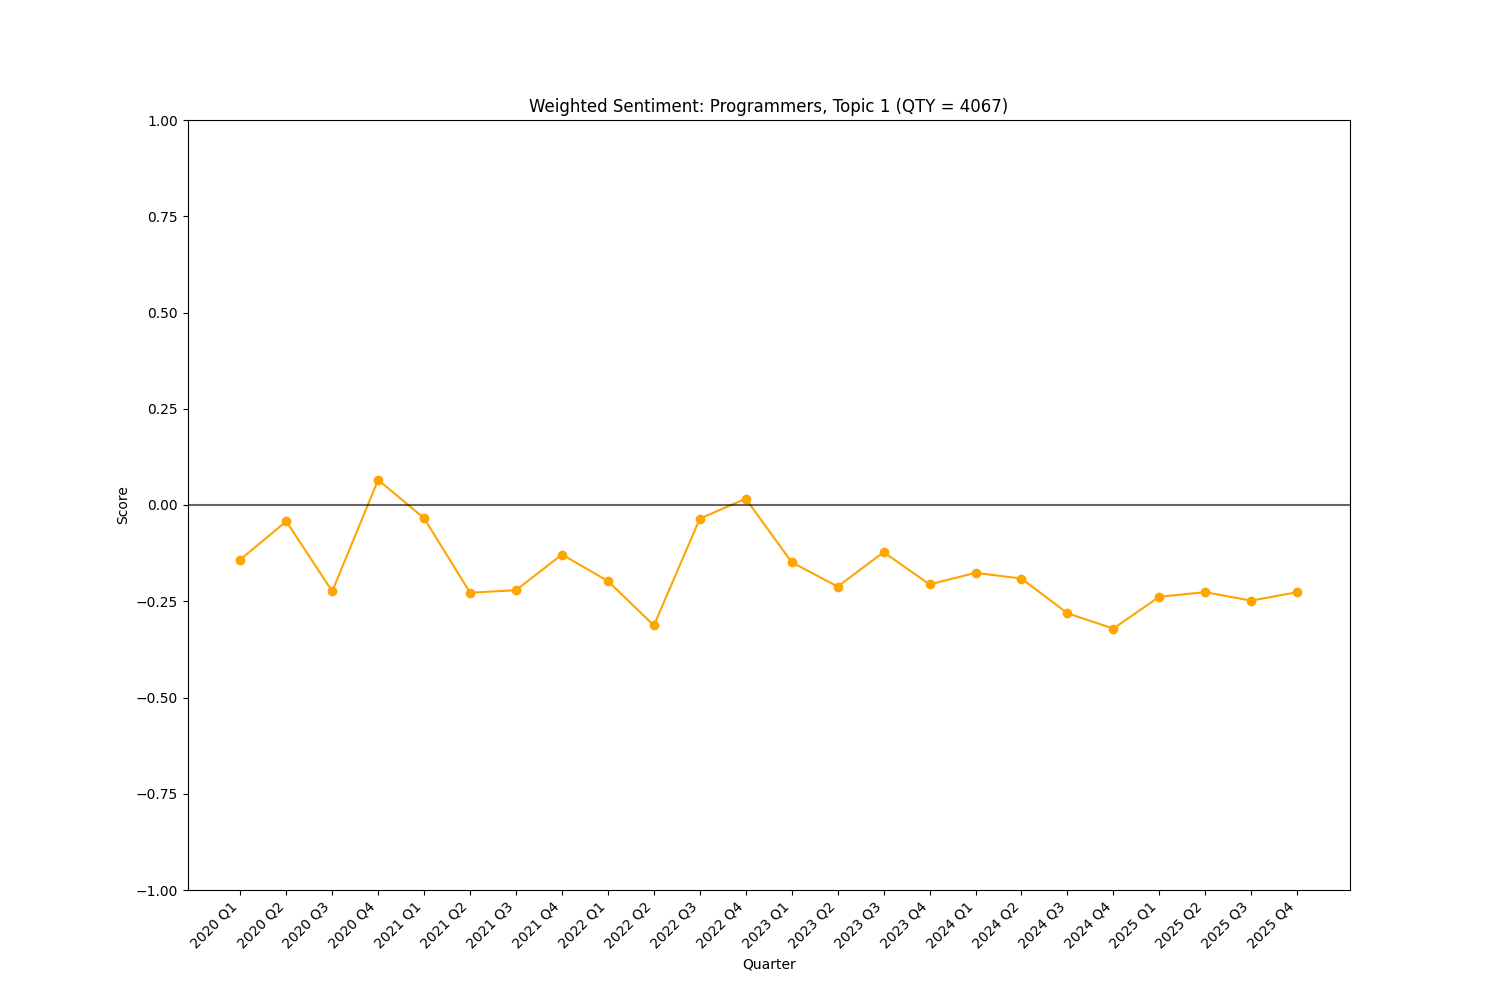
\includegraphics[width=0.80\linewidth]{Images/Appendices/Sentiment/Louvain/programmers_louvain_weighted_topic_1.png}
    \caption{Programmers topic 1}
\end{figure}
\begin{figure}[H]
    \centering
    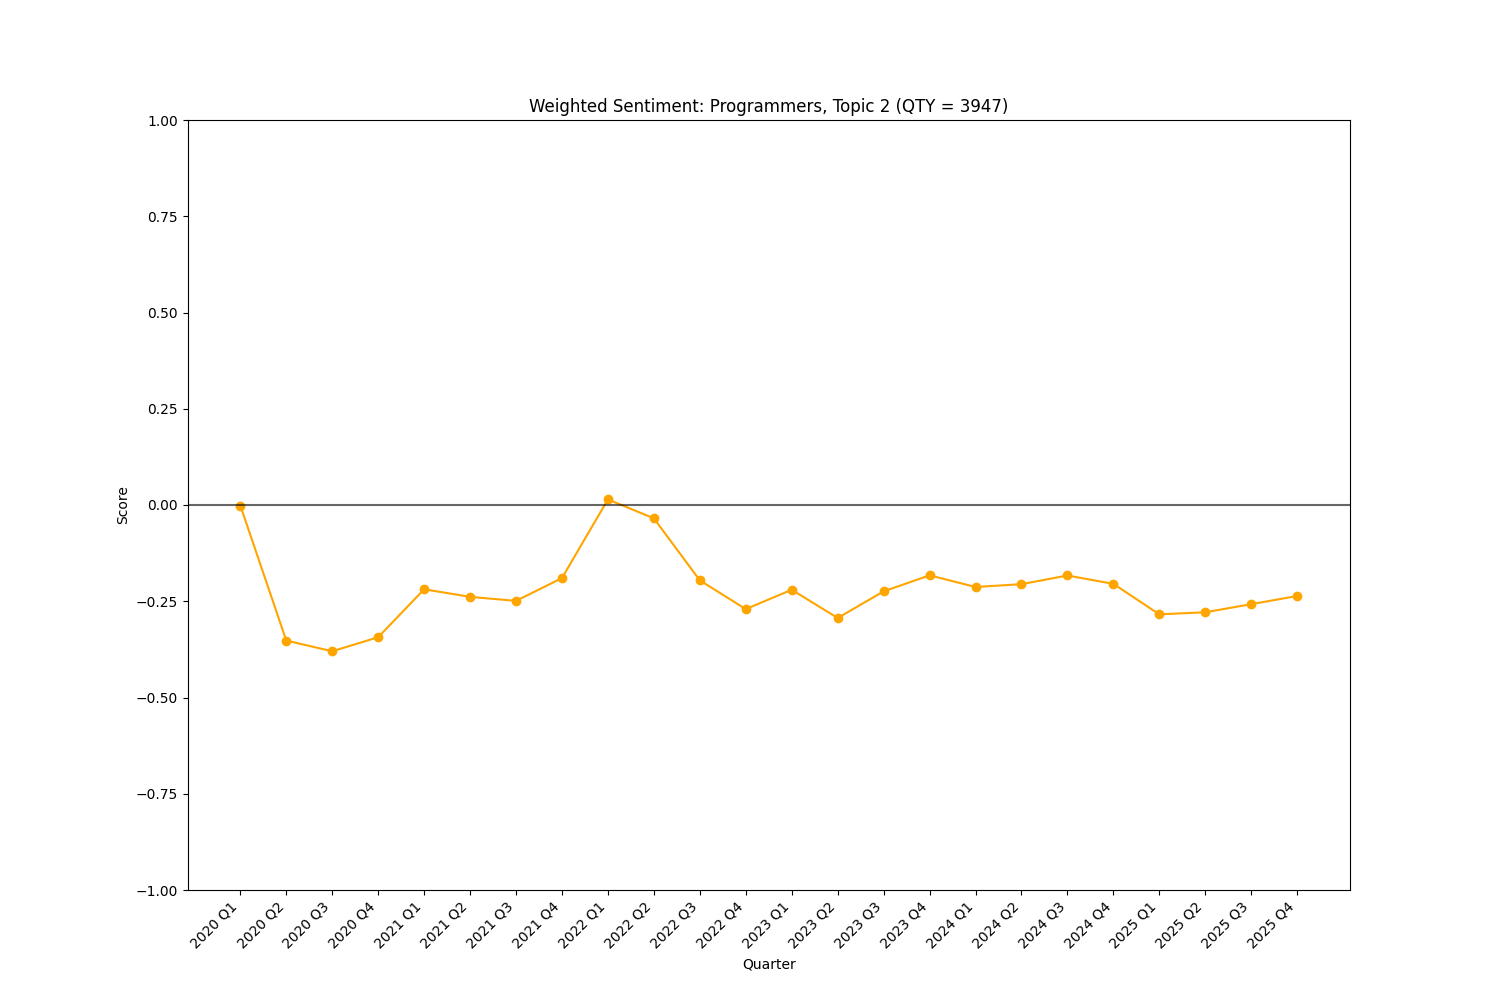
\includegraphics[width=0.80\linewidth]{Images/Appendices/Sentiment/Louvain/programmers_louvain_weighted_topic_2.png}
    \caption{Programmers topic 2}
\end{figure}
\begin{figure}[H]
    \centering
    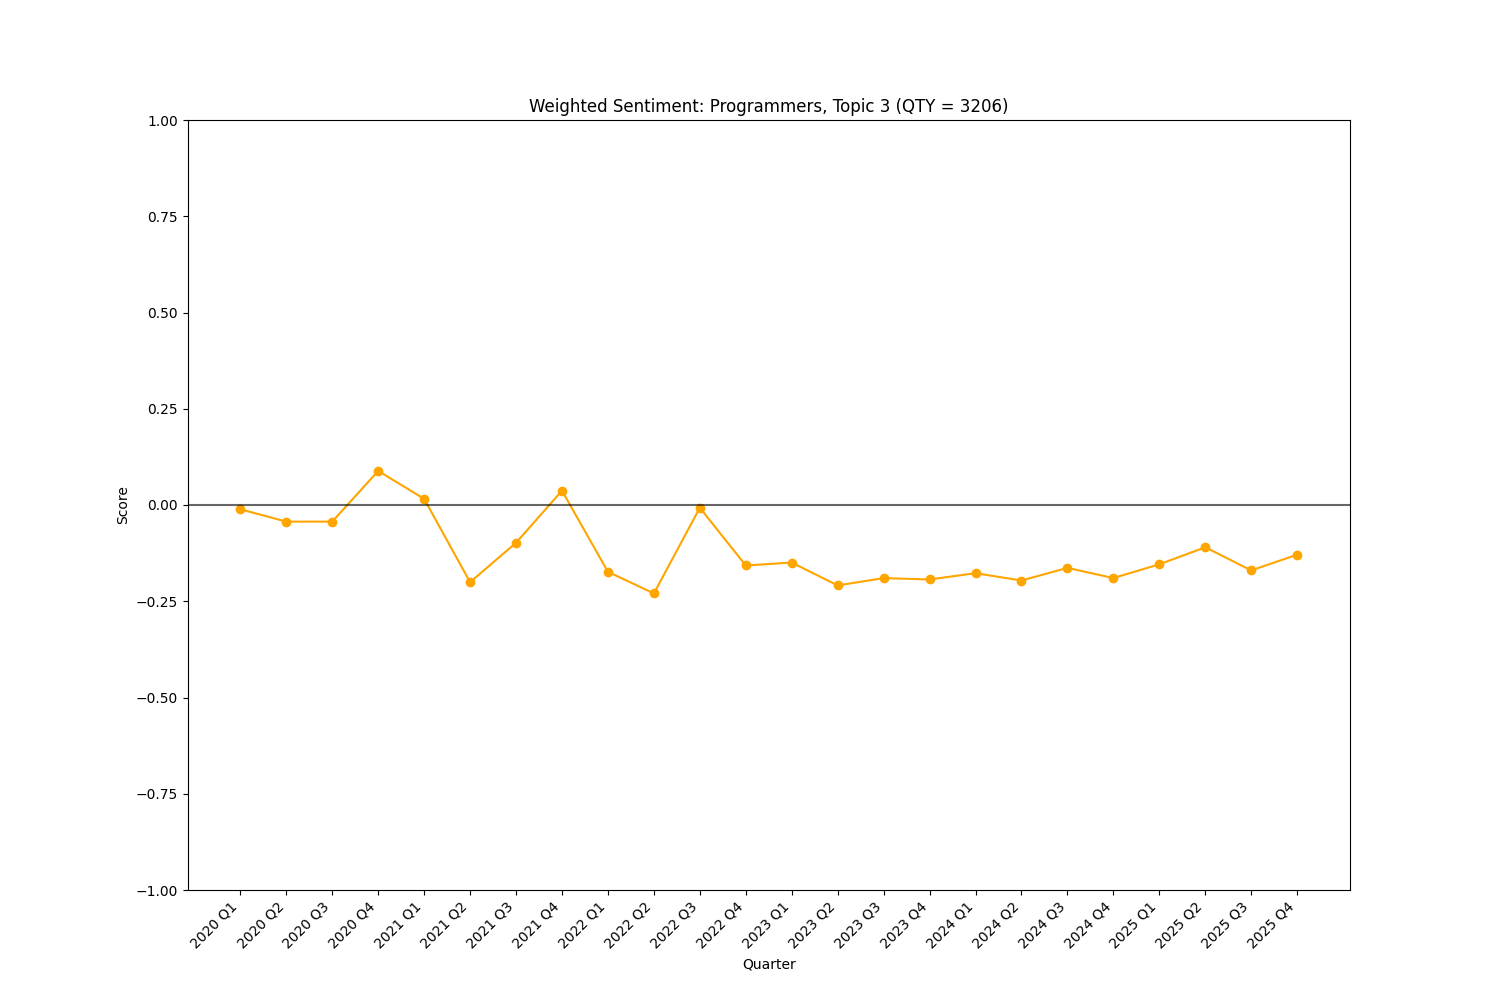
\includegraphics[width=0.80\linewidth]{Images/Appendices/Sentiment/Louvain/programmers_louvain_weighted_topic_3.png}
    \caption{Programmers topic 3}
\end{figure}
\begin{figure}[H]
    \centering
    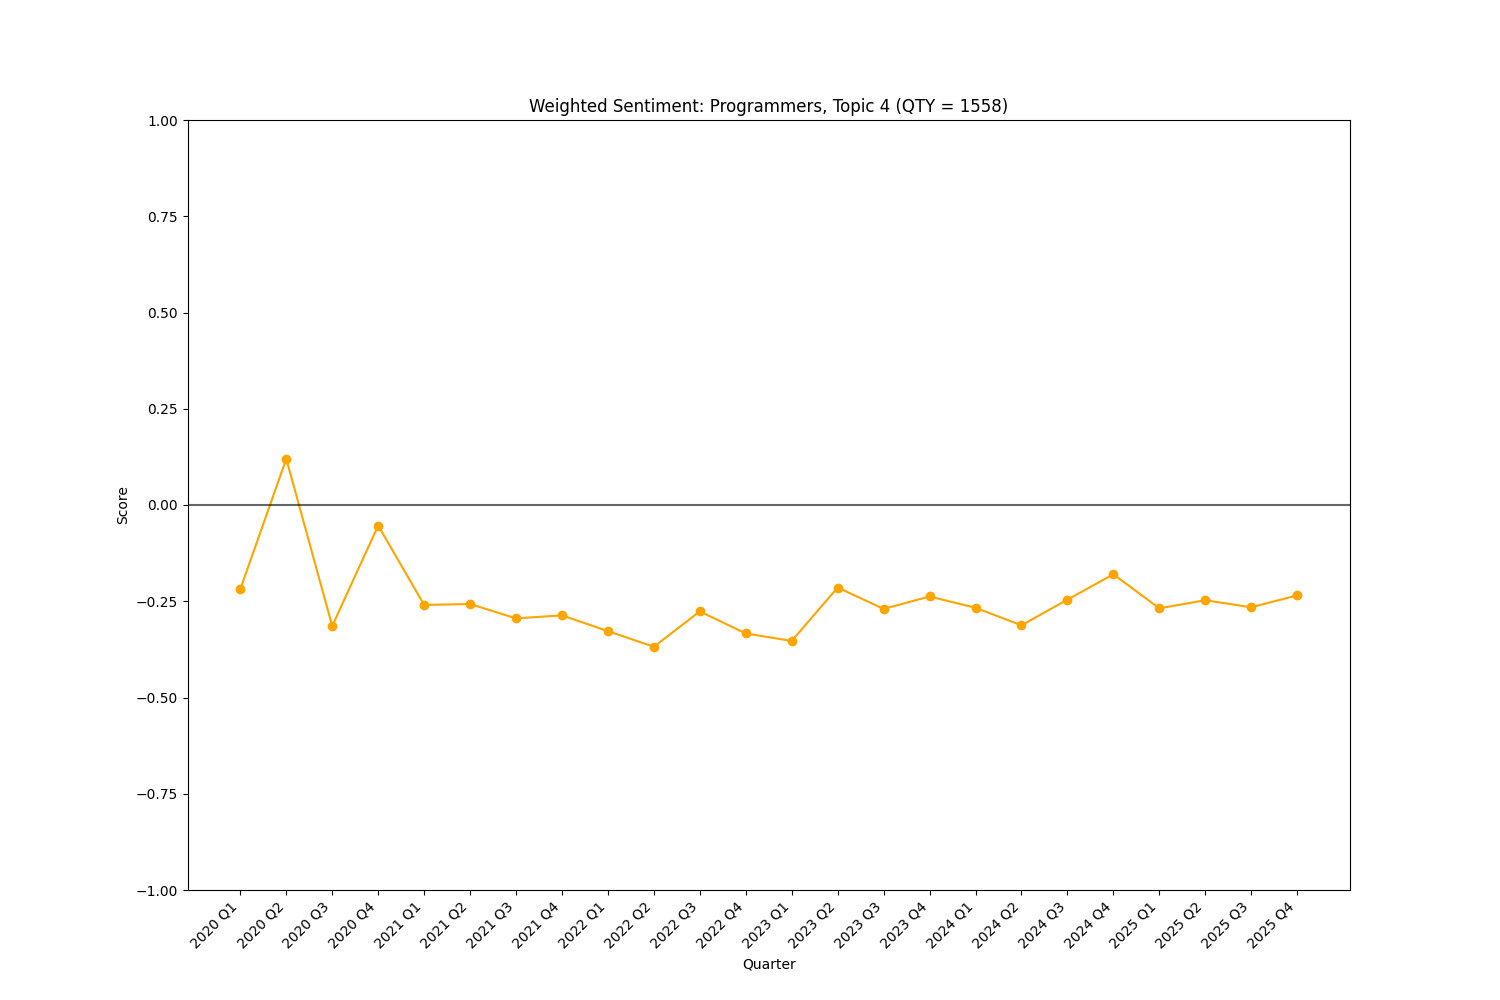
\includegraphics[width=0.80\linewidth]{Images/Appendices/Sentiment/Louvain/programmers_louvain_weighted_topic_4.png}
    \caption{Programmers topic 4}
\end{figure}

\end{document}